% !TeX program = xelatex
% Διπλωματική εργασία -- απαιτεί XeLaTeX (fontspec/polyglossia για ελληνικά).
% Μεταγλώττιση: xelatex thesis.tex  x3  (από μέσα από docs/)
\documentclass[12pt,a4paper,oneside]{report}

\usepackage{fontspec}
\usepackage{polyglossia}
\setmainlanguage{greek}
\setotherlanguage{english}
\setmainfont{Linux Libertine O}
\setsansfont{Linux Biolinum O}
\setmonofont{DejaVu Sans Mono}[Scale=0.85]

\usepackage[a4paper,margin=2.8cm]{geometry}
\usepackage{amsmath,amssymb,amsthm}
\usepackage{booktabs}
\usepackage{array}
\usepackage{float}
\usepackage{graphicx}
\graphicspath{{../results/}{./}}
\usepackage{enumitem}
\usepackage{caption}
\usepackage{xcolor}
\usepackage{longtable}
\usepackage[hidelinks]{hyperref}

\newcommand{\file}[1]{\texttt{#1}}
\newcommand{\en}[1]{\textenglish{#1}}
\let\oldunderscore\_
\renewcommand{\_}{\oldunderscore\allowbreak}
\setlength{\emergencystretch}{3em}
\setlist[itemize]{topsep=4pt,itemsep=3pt}

\theoremstyle{definition}
\newtheorem{definition}{Ορισμός}[chapter]
\theoremstyle{plain}
\newtheorem{theorem}{Θεώρημα}[chapter]
\newtheorem{lemma}[theorem]{Λήμμα}
\newtheorem{proposition}[theorem]{Πρόταση}
\newtheorem{corollary}[theorem]{Πόρισμα}
\theoremstyle{remark}
\newtheorem{remark}[theorem]{Παρατήρηση}

\begin{document}

% =====================================================================
% Εξώφυλλο
% =====================================================================
\begin{titlepage}
\centering
\vspace*{0.5cm}


\includegraphics[height=3.4cm]{tuc_logo.png}\par

\vspace{0.8cm}

{\large ΠΟΛΥΤΕΧΝΕΙΟ ΚΡΗΤΗΣ\par}
\vspace{0.35em}
{\normalsize ΣΧΟΛΗ ΗΛΕΚΤΡΟΛΟΓΩΝ ΜΗΧΑΝΙΚΩΝ ΚΑΙ ΜΗΧΑΝΙΚΩΝ ΥΠΟΛΟΓΙΣΤΩΝ\par}
\vspace{0.35em}
{\normalsize ΤΟΜΕΑΣ ΤΗΛΕΠΙΚΟΙΝΩΝΙΩΝ\par}

\vspace{2.4cm}

{\Large\bfseries Κυρτή Βελτιστοποίηση σε Πραγματικό Χρόνο\\[0.5em]
Βασισμένη στην Παραμετροποίηση Μείγματος Ειδικών\\[0.5em]
για την Πρόβλεψη Αποτελεσμάτων Αθλητικών Αγώνων\par}

\vspace{1.5cm}
{\large ΔΙΠΛΩΜΑΤΙΚΗ ΕΡΓΑΣΙΑ\par}
\vspace{1.1cm}
{\Large\bfseries Στέφανος Μουσάδης\par}

\vspace{2.0cm}

{\large ΕΞΕΤΑΣΤΙΚΗ ΕΠΙΤΡΟΠΗ\par}
\vspace{0.7em}
{\normalsize
Αναπληρωτής Καθηγητής Θρασύβουλος Σπυρόπουλος, \emph{Επιβλέπων}\\[0.4em]
Καθηγητής Μιχαήλ Γ. Λαγουδάκης\\[0.4em]
Αναπληρωτής Καθηγητής Βασίλειος Σαμολαδάς\par}

\vfill
{\large Χανιά, 2026\par}
\end{titlepage}

\cleardoublepage

% =====================================================================
% Περιλήψεις
% =====================================================================
\chapter*{Περίληψη}
\addcontentsline{toc}{chapter}{Περίληψη}

Η παρούσα εργασία προβλέπει τα αποτελέσματα αθλητικών αγώνων (1/Χ/2) ως πρόβλημα
\textbf{online μάθησης με συμβουλή ειδικών}, και όχι ως εκπαίδευση στατιστικού μοντέλου.
Κάθε στοιχηματικός πάροχος θεωρείται ένας expert που δίνει αποδόσεις για τα τρία ενδεχόμενα,
από τις οποίες προκύπτουν πιθανότητες. Ζητούμενο είναι η εύρεση ενός διανύσματος βαρών έτσι
ώστε το μείγμα των experts να τους ξεπερνά ατομικά, με μάθηση όχι αναδρομικά πάνω στο
παρελθόν, αλλά αγώνα προς αγώνα.

Υλοποιούνται τρία στάδια Κυρτής Βελτιστοποίησης σε Πραγματικό Χρόνο (\textbf{Online Convex
Optimization}, OCO). Αρχικά κατασκευάζονται τρεις αλγόριθμοι (Hedge, Online Gradient Descent,
Follow-The-Regularized-Leader), που με την αναγωγή σε \textbf{Sleeping Experts} διαχειρίζονται
τους παρόχους μερικής κάλυψης. Έπειτα, με δεύτερο στάδιο OCO, γίνεται βαθμονόμηση μέσω online
temperature scaling. Τέλος υπολογίζεται το μέγεθος του στοιχήματος με το κριτήριο Kelly, όπου
ο πολλαπλασιαστής του μαθαίνεται online με Online Newton Step. Κάθε σύγκριση ελέγχεται με
moving block bootstrap. Το σύνολο δεδομένων καλύπτει 22 πρωταθλήματα, 10 σεζόν και 76.584
αγώνες.

Το μείγμα ξεπερνά στατιστικά σημαντικά κάθε μεμονωμένο bookmaker πλην του σκληρότερου, με
τον οποίο ισοπαλεί στη διαμόρφωση που επιλέγεται τελικά. Σε έλεγχο ανάπτυξης με πραγματική
χρονική τομή --- εκπαίδευση έως το τέλος του 2024, μέτρηση στο 2025--26 --- ξεπερνά ή
ισοπαλεί με κάθε τιμή της αγοράς: κερδίζει σημαντικά όλες τις τιμές ανοίγματος και ισοπαλεί
με όλες τις τιμές κλεισίματος, χωρίς καμία να το ξεπερνά.

Τα τρία γενικότερα ευρήματα είναι ότι η μάθηση αποδίδει μόνο όταν οι experts έχουν
ανομοιομορφία στην ποιότητα, ότι η καλύτερη πρόβλεψη δεν μεταφράζεται άμεσα σε κέρδος καθώς
η διαφορά ποιότητας υπολείπεται του περιθωρίου της αγοράς, και ότι ένα μέρος της υπεροχής
έναντι της ομοιόμορφης μέσης τιμής δεν οφείλεται στη μάθηση αλλά στη γεωμετρία της αναγωγής
Sleeping Experts.

\vspace{1em}
\noindent\textbf{Λέξεις-κλειδιά:} online κυρτή βελτιστοποίηση, πρόβλεψη με συμβουλή ειδικών,
sleeping experts, regret, βαθμονόμηση πιθανοτήτων, αγορές στοιχηματισμού

\cleardoublepage

\begin{english}
\chapter*{Abstract}
\addcontentsline{toc}{chapter}{Abstract}

This thesis predicts sports match outcomes (home / draw / away) as a problem of
\textbf{online learning with expert advice}, rather than as the training of a statistical
model. Each betting operator is treated as an expert quoting odds on the three outcomes,
from which probabilities are derived. The task is to find a weight vector such that the
mixture of experts outperforms each of them individually, learning not retrospectively over
the past but match by match.

Three stages of \textbf{Online Convex Optimization} (OCO) are implemented. First, three
algorithms are built (Hedge, Online Gradient Descent, Follow-The-Regularized-Leader), which
handle partially covering operators through the \textbf{Sleeping Experts} reduction. A second
OCO stage then calibrates the mixture via online temperature scaling. Finally the bet size is
computed with the Kelly criterion, whose multiplier is itself learned online with Online
Newton Step. Every comparison is tested with a moving block bootstrap. The dataset spans
22 leagues, 10 seasons and 76,584 matches.

The mixture significantly outperforms every individual bookmaker except the sharpest, with
which it draws level in the configuration ultimately adopted. Under a deployment test with a
genuine temporal cut --- fitted through the end of 2024, evaluated on 2025--26 --- it
matches or beats every price in the market: it significantly outperforms all opening prices
and draws level with all closing prices, with none of them outperforming it.

The three broader findings are that learning pays only where experts are heterogeneous in
quality; that better prediction does not translate directly into profit, since the quality
gain falls short of the market's margin; and that part of the advantage over the uniform
average is due not to learning but to the geometry of the Sleeping Experts reduction.

\vspace{1em}
\noindent\textbf{Keywords:} online convex optimization, prediction with expert advice,
sleeping experts, regret, probability calibration, betting markets
\end{english}

\cleardoublepage
\tableofcontents
\cleardoublepage

% =====================================================================
\chapter{Εισαγωγή}
% =====================================================================

\section{Το πρόβλημα}

Η πρόβλεψη του αποτελέσματος ενός ποδοσφαιρικού αγώνα αντιμετωπίζεται συνήθως ως πρόβλημα
επιβλεπόμενης μάθησης: συγκεντρώνονται χαρακτηριστικά των ομάδων και των αγώνων,
εκπαιδεύεται ένα μοντέλο, και αξιολογείται σε δεδομένα που δεν έχει δει. Η προσέγγιση αυτή
προσκρούει σε έναν πρακτικό φραγμό. Οι στοιχηματικές εταιρείες λύνουν ήδη το ίδιο πρόβλημα,
με ασύγκριτα περισσότερα δεδομένα, με ομάδες αναλυτών και με άμεσο οικονομικό κίνητρο να το
λύσουν σωστά. Ένα μοντέλο εκπαιδευμένο στο πλαίσιο μιας διπλωματικής δύσκολα θα τις
ανταγωνιστεί στο έδαφός τους.

Η εργασία αυτή αλλάζει το ερώτημα. Αντί να χτίσει έναν ακόμη προγνώστη, αντιμετωπίζει
\emph{κάθε στοιχηματική εταιρεία ως έναν expert} που δημοσιεύει, πριν από κάθε αγώνα, τις
δικές του πιθανότητες $(p_H, p_D, p_A)$ για τα τρία ενδεχόμενα. Το ζητούμενο γίνεται τότε:
πώς συνδυάζονται αυτές οι γνώμες, online και χωρίς γνώση του μέλλοντος, ώστε το μείγμα να
είναι καλύτερος προγνώστης από τον καθένα τους χωριστά;

Το πλαίσιο που απαντά σε αυτό είναι η \emph{πρόβλεψη με συμβουλή ειδικών} (\en{prediction
with expert advice}) και, γενικότερα, η \emph{online κυρτή βελτιστοποίηση} (\en{Online
Convex Optimization}, OCO). Το βασικό του πλεονέκτημα εδώ είναι ότι δίνει εγγυήσεις regret
\textbf{χωρίς καμία στατιστική υπόθεση} για την κατανομή των δεδομένων: δεν απαιτείται τα
αποτελέσματα να προέρχονται από σταθερή κατανομή, ούτε οι experts να είναι ανεξάρτητοι.
Αυτό ταιριάζει σε μια αγορά που μεταβάλλεται, όπου εταιρείες εμφανίζονται και εξαφανίζονται
και όπου οι τιμές διαμορφώνονται στρατηγικά.

\section{Γιατί δεν είναι τετριμμένο}

Η εφαρμογή του πλαισίου σε πραγματικά δεδομένα συναντά τρεις δυσκολίες που καθορίζουν τη
δομή της εργασίας.

\paragraph{Μερική κάλυψη.} Οι κλασικοί αλγόριθμοι υποθέτουν ότι κάθε expert δίνει πρόβλεψη
σε κάθε γύρο. Στην πράξη, στα δεδομένα που χρησιμοποιούμε, η κάλυψη ανά bookmaker κυμαίνεται
από 6,9\% έως 99,8\% των αγώνων, και αρκετές εταιρείες εμφανίζονται ή εξαφανίζονται στη μέση
της δεκαετίας. Χρειάζεται η αναγωγή \emph{Sleeping Experts}, που αντιστοιχίζει σε κάθε
expert εγγύηση μετρημένη μόνο πάνω στους γύρους όπου ήταν παρών.

\paragraph{Οι αποδόσεις δεν είναι πιθανότητες.} Οι δημοσιευμένες αποδόσεις ενσωματώνουν το
περιθώριο κέρδους του bookmaker: τα αντίστροφά τους αθροίζουν σε περισσότερο από ένα. Η
μετατροπή τους σε πιθανότητες (\en{de-vig}) είναι μοντελοποιητική επιλογή που μπορεί να
επηρεάσει τα συμπεράσματα, και γι' αυτό ελέγχεται με δύο ανεξάρτητες μεθόδους.

\paragraph{Το καλύτερο log-loss δεν είναι το ζητούμενο.} Ένα μείγμα μπορεί να προβλέπει
καλύτερα από κάθε bookmaker και να χάνει χρήματα, αν η υπεροχή του είναι μικρότερη από το
περιθώριο της αγοράς. Η εργασία ελέγχει ρητά αυτό το χάσμα, με προσομοίωση στοιχηματισμού
βασισμένη στο κριτήριο Kelly.

\section{Συνεισφορά}

Η εργασία συνεισφέρει τα εξής.

\begin{itemize}
  \item Πλήρη υλοποίηση τριών αλγορίθμων OCO με την αναγωγή Sleeping Experts, πάνω σε
        σύνολο 22 πρωταθλημάτων, 10 σεζόν και 76.584 αγώνων, με 26 bookmakers ως experts.
  \item Δύο επιπλέον στάδια OCO πάνω στο μείγμα: βαθμονόμηση με online temperature scaling
        και μέγεθος στοιχήματος με μαθαινόμενο πολλαπλασιαστή Kelly, ώστε ολόκληρη η αλυσίδα
        από τις αποδόσεις ως το στοίχημα να είναι online και αιτιώδης. Δείχνεται ότι το
        \emph{τι} μαθαίνεται στο τρίτο στάδιο είναι καθοριστικό: η μάθηση του πονταρίσματος
        κατευθείαν αποτυγχάνει συστηματικά, ενώ η μάθηση του πολλαπλασιαστή πάνω στον
        κλειστό τύπο όχι.
  \item Συστηματικό στατιστικό έλεγχο κάθε σύγκρισης με moving block bootstrap, αντί για
        σύγκριση σημειακών εκτιμήσεων.
  \item Έλεγχο ανάπτυξης με πραγματική χρονική τομή, που απαντά στο ερώτημα «τι θα έκανε
        σήμερα ένα μοντέλο εκπαιδευμένο ως το 2024».
  \item Μια σειρά αρνητικών ευρημάτων που περιορίζουν το πεδίο εφαρμογής της μεθόδου και
        είναι, κατά τη γνώμη μας, εξίσου χρήσιμα με τα θετικά.
\end{itemize}

\section{Δομή}

Το Κεφάλαιο~\ref{ch:theory} αναπτύσσει το θεωρητικό υπόβαθρο. Το Κεφάλαιο~\ref{ch:data}
περιγράφει τα δεδομένα και την προεπεξεργασία τους. Το Κεφάλαιο~\ref{ch:method} παρουσιάζει
τη μεθοδολογία και τις αποφάσεις σχεδιασμού. Το Κεφάλαιο~\ref{ch:results} δίνει τα
αποτελέσματα και το Κεφάλαιο~\ref{ch:discussion} τα συζητά, μαζί με τα όρια της μεθόδου. Το
Κεφάλαιο~\ref{ch:conclusion} συνοψίζει και προτείνει επεκτάσεις.

% =====================================================================
\chapter{Σχετική βιβλιογραφία}
\label{ch:related}
% =====================================================================

Η εργασία τοποθετείται στη συμβολή τριών ερευνητικών παραδόσεων που αναπτύχθηκαν σε μεγάλο
βαθμό ανεξάρτητα: της θεωρίας online μάθησης, της πρόβλεψης αθλητικών αποτελεσμάτων, και της
οικονομικής μελέτης των αγορών στοιχηματισμού. Το κεφάλαιο αυτό σκιαγραφεί καθεμία και
προσδιορίζει πού εντάσσεται η παρούσα συνεισφορά.

\section{Online μάθηση και θεωρία regret}

Η ιδέα της πρόβλεψης με συμβουλή ειδικών προηγείται της σύγχρονης μηχανικής μάθησης. Στην
υπολογιστική της μορφή εμφανίζεται με τον αλγόριθμο \emph{weighted majority} των Littlestone
\& Warmuth (1994), που έδειξε ότι είναι δυνατόν να εγγυηθεί κανείς απόδοση σχεδόν όσο καλή
όσο του καλύτερου expert ενός συνόλου, χωρίς καμία υπόθεση για το πώς παράγονται τα δεδομένα.
Η γενίκευση σε συνεχή βάρη και σε κυρτές απώλειες οδήγησε στον Hedge και στην οικογένεια των
πολλαπλασιαστικών ενημερώσεων.

Παράλληλα αναπτύχθηκε η ιδέα της \emph{αθροιστικής στρατηγικής} (\en{aggregating algorithm})
του Vovk (1990), η οποία εκμεταλλεύεται μια ισχυρότερη ιδιότητα ορισμένων απωλειών, την
\emph{exp-concavity}. Όταν η απώλεια είναι exp-concave --- όπως είναι το log-loss --- το
regret μπορεί να φραχθεί από $\ln N$, δηλαδή \emph{ανεξάρτητα} από τον ορίζοντα $T$, αντί
για $O(\sqrt{T \log N})$. Το αποτέλεσμα αυτό είναι θεωρητικά ισχυρότερο, και η εργασία μας
προσφέρει ένα εμπειρικό παράδειγμα όπου εντούτοις αποτυγχάνει, για λόγους που συνδέονται με
τη μη στασιμότητα του συνόλου των experts.

Η ενοποίηση των παραπάνω κάτω από τον κοινό τίτλο της \emph{online κυρτής βελτιστοποίησης}
οφείλεται σε μεγάλο βαθμό στον Zinkevich (2003), ο οποίος έδειξε ότι η απλή προβολική
κατάβαση κλίσης επιτυγχάνει regret $O(\sqrt{T})$ για οποιαδήποτε ακολουθία κυρτών
συναρτήσεων. Οι σύγχρονες συνθετικές παρουσιάσεις του πεδίου δίνονται από τους Cesa-Bianchi
\& Lugosi (2006) και Hazan (2016).

Δύο επεκτάσεις είναι άμεσα σχετικές με την εφαρμογή μας. Η πρώτη είναι η αναγωγή
\emph{sleeping experts} ή \emph{specialists} (Freund, Schapire, Singer \& Warmuth, 1997·
Blum \& Mansour, 2007), που αντιμετωπίζει experts οι οποίοι δεν συμμετέχουν σε κάθε γύρο. Η
δεύτερη είναι το \emph{Fixed-Share} των Herbster \& Warmuth (1998), το οποίο αλλάζει τον
comparator από το καλύτερο σταθερό διάνυσμα στην καλύτερη ακολουθία διανυσμάτων με
περιορισμένο πλήθος αλλαγών, και άρα απευθύνεται ακριβώς στο πρόβλημα της μη στασιμότητας.

Τέλος, οι προσαρμοστικοί ρυθμοί μάθησης τύπου AdaGrad (Duchi, Hazan \& Singer, 2011)
προτείνουν ανά συντεταγμένη κλιμάκωση του βήματος με βάση τη συσσωρευμένη κλίση. Η ιδέα
είναι ελκυστική σε ένα πλαίσιο όπου οι experts έχουν πολύ διαφορετική συχνότητα συμμετοχής,
και εξετάζεται ρητά στο \S\ref{sec:res-negative}.

\section{Πρόβλεψη αθλητικών αποτελεσμάτων}

Η βιβλιογραφία της πρόβλεψης ποδοσφαιρικών αποτελεσμάτων ακολουθεί, χονδρικά, τρεις
κατευθύνσεις.

Η πρώτη είναι τα \emph{παραμετρικά στατιστικά μοντέλα}, με αφετηρία την παρατήρηση ότι τα
γκολ προσεγγίζονται ικανοποιητικά από κατανομή Poisson. Τα μοντέλα αυτά εκτιμούν επιθετική
και αμυντική ισχύ ανά ομάδα και παράγουν κατανομή σκορ, από την οποία προκύπτουν οι
πιθανότητες 1/Χ/2. Το βασικό τους πλεονέκτημα είναι η ερμηνευσιμότητα· το βασικό τους
μειονέκτημα ότι απαιτούν επαρκές ιστορικό ανά ομάδα και δυσκολεύονται με μεταγραφές,
αλλαγές προπονητή και ανόδους/υποβιβασμούς.

Η δεύτερη είναι η \emph{μηχανική μάθηση πάνω σε χαρακτηριστικά}, όπου συγκεντρώνονται
μεταβλητές μορφής, κατάταξης, στατιστικών αναμέτρησης και, στις πιο πρόσφατες εργασίες,
δεδομένα παρακολούθησης παικτών. Τα μοντέλα αυτά συχνά αποδίδουν καλά σε σύγκριση με
παραμετρικές εναλλακτικές, αλλά η σύγκρισή τους με την αγορά είναι σπανιότερη και συνήθως
λιγότερο αυστηρή.

Η τρίτη, και η σχετικότερη εδώ, χρησιμοποιεί \emph{τις ίδιες τις αποδόσεις ως πρόβλεψη}. Η
προσέγγιση αυτή αναγνωρίζει ότι η τιμή της αγοράς ενσωματώνει το σύνολο της διαθέσιμης
πληροφορίας, συμπεριλαμβανομένων στοιχείων που δεν αποτυπώνονται σε δημόσια στατιστικά. Η
παρούσα εργασία ανήκει σε αυτή την κατηγορία, με τη διαφορά ότι δεν χρησιμοποιεί μία τιμή
αλλά μαθαίνει online πώς να συνδυάζει πολλές.

\section{Αποδοτικότητα αγορών στοιχηματισμού}

Οι αγορές στοιχηματισμού αποτελούν προνομιακό πεδίο μελέτης της αποδοτικότητας των αγορών,
για έναν συγκεκριμένο λόγο: σε αντίθεση με τις χρηματοπιστωτικές αγορές, κάθε στοίχημα έχει
\emph{καθορισμένη ημερομηνία λήξης και αντικειμενικά επαληθεύσιμο αποτέλεσμα}. Η
θεμελιώδης αξία δεν χρειάζεται να εκτιμηθεί· αποκαλύπτεται.

Ο Levitt (2004) τεκμηριώνει ότι οι αγορές στοιχηματισμού οργανώνονται διαφορετικά από τις
χρηματοπιστωτικές: ο bookmaker δεν λειτουργεί απλώς ως μεσάζων που εξισορροπεί τις δύο
πλευρές, αλλά λαμβάνει ενεργή θέση, εκμεταλλευόμενος συστηματικές προκαταλήψεις των
στοιχηματιστών. Η παρατήρηση αυτή είναι σημαντική για την ερμηνεία των διαφορών ανάμεσα στις
εταιρείες: δεν αντανακλούν μόνο διαφορετική ικανότητα πρόβλεψης αλλά και διαφορετική
επιχειρηματική στρατηγική.

Η θεωρία μικροδομής της αγοράς προσφέρει το πλαίσιο για την κατανόηση του τρόπου με τον οποίο
η πληροφορία ενσωματώνεται στην τιμή. Τα υποδείγματα των Kyle (1985) και Glosten \& Milgrom
(1985) δείχνουν ότι, παρουσία πληροφορημένων συναλλασσομένων, η κίνηση της τιμής είναι ο
μηχανισμός μέσω του οποίου η ιδιωτική πληροφορία γίνεται δημόσια, και ότι το άνοιγμα
τιμής--προσφοράς λειτουργεί ως προστασία του διαμορφωτή έναντι αυτών. Το πλαίσιο αυτό
φωτίζει άμεσα τη διαφορά ανάμεσα σε τιμές ανοίγματος και κλεισίματος
(\S\ref{sec:openclose}).

\section{Favorite-longshot bias και μετατροπή αποδόσεων}

Η συστηματικότερα τεκμηριωμένη ανωμαλία των αγορών στοιχηματισμού είναι το
\emph{favorite-longshot bias}: τα ενδεχόμενα μικρής πιθανότητας τιμολογούνται συστηματικά
ακριβότερα απ' όσο δικαιολογεί η πραγματική τους συχνότητα. Το φαινόμενο έχει επιβεβαιωθεί
σε πολλαπλά αθλήματα και δεκαετίες.

Ο Shin (1992, 1993) προσέφερε μια εξήγηση που δεν το αντιμετωπίζει ως ψυχολογική
προκατάληψη των στοιχηματιστών αλλά ως \emph{ορθολογική απόκριση} του bookmaker στην ύπαρξη
πληροφορημένων συναλλασσομένων. Το υπόδειγμα παράγει ενδογενώς τη μορφή του bias και, το
σημαντικότερο για εμάς, δίνει μια διαδικασία αντιστροφής που ανακτά τις δίκαιες πιθανότητες
μαζί με μια εκτίμηση της αναλογίας $z$ των πληροφορημένων. Ο Štrumbelj (2014) συγκρίνει
συστηματικά τις μεθόδους μετατροπής αποδόσεων σε πιθανότητες και βρίσκει ότι η μέθοδος Shin
υπερέχει της αναλογικής κανονικοποίησης ως προς την ποιότητα των προκυπτουσών πιθανοτήτων.

\section{Βαθμονόμηση πιθανοτήτων}

Η διάκριση ανάμεσα στην \emph{αξιοπιστία} και τη \emph{διακριτική ικανότητα} μιας
πιθανοτικής πρόβλεψης ανάγεται στον Murphy (1973), ο οποίος έδειξε ότι κάθε κατάλληλος
κανόνας βαθμολόγησης αναλύεται σε αυτές τις συνιστώσες. Η παρατήρηση έχει άμεση πρακτική
συνέπεια: ένας προγνώστης μπορεί να διακρίνει άριστα ανάμεσα σε πιθανά και απίθανα
ενδεχόμενα και εντούτοις να αποδίδει λανθασμένες πιθανότητες, σφάλμα διορθώσιμο χωρίς καμία
επιπλέον πληροφορία.

Στη σύγχρονη βιβλιογραφία της μηχανικής μάθησης το ζήτημα επανήλθε με τους Guo κ.ά. (2017),
οι οποίοι έδειξαν ότι τα βαθιά νευρωνικά δίκτυα είναι συστηματικά υπερβέβαια και ότι μια
μονοπαραμετρική διόρθωση --- το \emph{temperature scaling} --- αρκεί για να τα
βαθμονομήσει. Η παρούσα εργασία χρησιμοποιεί την ίδια οικογένεια διόρθωσης, με τη διαφορά
ότι η παράμετρος δεν προσαρμόζεται σε σύνολο επικύρωσης αλλά μαθαίνεται \emph{online},
ως δεύτερο στάδιο OCO πάνω στο πρώτο.

\section{Συνδυασμός προβλέψεων}

Η ιδέα ότι ο συνδυασμός πολλών προβλέψεων υπερέχει της επιλογής μίας έχει μακρά ιστορία στην
οικονομετρία και τη μετεωρολογία. Ένα σταθερό εμπειρικό εύρημα, γνωστό ως
\emph{forecast combination puzzle}, είναι ότι ο απλός μέσος όρος συχνά αποδεικνύεται
ανθεκτικότερος από σταθμισμένους συνδυασμούς με βάρη εκτιμημένα από τα δεδομένα: το κέρδος
από τη βελτιωμένη στάθμιση αναιρείται από τον θόρυβο εκτίμησης των βαρών.

Το εύρημα αυτό είναι άμεσα σχετικό με τα αποτελέσματά μας. Η εργασία δείχνει ότι ο
συνδυασμός με μάθηση υπερέχει του απλού μέσου όρου όταν οι experts διαφέρουν ουσιωδώς σε
ποιότητα, και υπολείπεται αυτού όταν δεν διαφέρουν --- δηλαδή προσδιορίζει εμπειρικά τη
συνθήκη υπό την οποία το puzzle ισχύει ή όχι.

\section{Θέση της παρούσας εργασίας}

Από τον συνδυασμό των παραπάνω προκύπτει το κενό στο οποίο απευθύνεται η εργασία. Η θεωρία
online μάθησης προσφέρει αλγορίθμους με εγγυήσεις αλλά εφαρμόζεται σπανιότερα σε αγορές
στοιχηματισμού με πραγματική μερική κάλυψη. Η βιβλιογραφία πρόβλεψης αθλητικών
αποτελεσμάτων χρησιμοποιεί συχνά τις αποδόσεις ως σημείο αναφοράς, αλλά λιγότερο συχνά ως
\emph{σύνολο experts προς συνδυασμό}. Και η οικονομική βιβλιογραφία των αγορών εξηγεί γιατί
οι εταιρείες διαφέρουν, αλλά δεν αξιοποιεί αυτές τις διαφορές αλγοριθμικά.

Η συνεισφορά μας είναι η συστηματική σύνθεση των τριών: online αλγόριθμοι με εγγυήσεις,
εφαρμοσμένοι στο πλήρες σύνολο των διαθέσιμων εταιρειών με τη σωστή αντιμετώπιση της μερικής
κάλυψης, με στατιστικό έλεγχο κάθε σύγκρισης και με ρητή διάκριση ανάμεσα στην προγνωστική
και στην οικονομική επίδοση.

% =====================================================================
\chapter{Θεωρητικό υπόβαθρο}
\label{ch:theory}
% =====================================================================

\section{Online μάθηση και regret}

Στο πλαίσιο της online μάθησης δεν υπάρχει διαχωρισμός σε φάση εκπαίδευσης και φάση
εφαρμογής. Ο αλγόριθμος λειτουργεί σε γύρους: στον γύρο $t$ διατυπώνει μια πρόβλεψη με βάση
μόνο ό,τι έχει δει ως τον γύρο $t-1$, στη συνέχεια αποκαλύπτεται το πραγματικό αποτέλεσμα,
υφίσταται μια απώλεια, και ενημερώνει την κατάστασή του. Κάθε πρόβλεψη είναι επομένως εξ
ορισμού εκτός δείγματος, χωρίς να χρειάζεται διαχωρισμός των δεδομένων.

Το μέτρο επιτυχίας δεν είναι η απόλυτη απώλεια αλλά το \emph{regret}: πόσο χειρότερα τα πήγε
ο αλγόριθμος από την καλύτερη \emph{σταθερή} επιλογή εκ των υστέρων.

\begin{definition}[Regret]
Έστω κυρτό σύνολο $\mathcal{K}$, ακολουθία κυρτών συναρτήσεων απώλειας $f_1,\dots,f_T$, και
επιλογές $x_1,\dots,x_T \in \mathcal{K}$ του αλγορίθμου, όπου το $x_t$ εξαρτάται μόνο από τα
$f_1,\dots,f_{t-1}$. Το regret ορίζεται ως
\[
\mathrm{Regret}_T \;=\; \sum_{t=1}^{T} f_t(x_t) \;-\; \min_{x \in \mathcal{K}} \sum_{t=1}^{T} f_t(x).
\]
\end{definition}

Ένας αλγόριθμος θεωρείται επιτυχής όταν το regret του αυξάνεται υπογραμμικά ως προς $T$,
δηλαδή $\mathrm{Regret}_T / T \to 0$: μακροπρόθεσμα η μέση απώλειά του πλησιάζει αυτήν της
καλύτερης σταθερής επιλογής. Κρίσιμο για την εφαρμογή μας είναι ότι η εγγύηση αυτή ισχύει
\textbf{για κάθε} ακολουθία, χωρίς υπόθεση ανεξαρτησίας ή σταθερότητας της κατανομής.

Το σημείο αυτό αξίζει να διατυπωθεί με ακρίβεια, γιατί είναι ο λόγος για τον οποίο
επιλέγεται εδώ το πλαίσιο OCO αντί του στατιστικού. Στη στατιστική θεωρία μάθησης το
ζητούμενο είναι φράγμα στο \emph{risk} $\mathbb{E}_{(x,y)\sim\mathcal{D}}[\ell(h(x),y)]$, το
οποίο προϋποθέτει ότι υπάρχει σταθερή κατανομή $\mathcal{D}$ και ότι τα δείγματα αντλούνται
ανεξάρτητα από αυτήν. Καμία από τις δύο υποθέσεις δεν είναι αβλαβής εδώ: οι αποδόσεις
διαμορφώνονται από μια αγορά που μεταβάλλεται μέσα στη δεκαετία, και διαδοχικοί αγώνες
μοιράζονται αγωνιστική, πρωτάθλημα και περίοδο. Το regret δεν χρειάζεται καμία από τις δύο.
Το τίμημα είναι ότι η εγγύηση γίνεται \emph{σχετική}: δεν λέει ότι θα προβλέψουμε καλά, αλλά
ότι δεν θα προβλέψουμε ουσιωδώς χειρότερα από τον καλύτερο σταθερό συνδυασμό των experts.
Αν όλοι οι experts είναι κακοί, η εγγύηση τηρείται και το αποτέλεσμα παραμένει κακό.

\paragraph{Το πρωτόκολλο.} Τυπικά, η online κυρτή βελτιστοποίηση είναι το εξής παίγνιο
μεταξύ του αλγορίθμου και ενός --- εν δυνάμει εχθρικού --- περιβάλλοντος:

\begin{quote}
\textbf{για} $t = 1,2,\dots,T$:\\[2pt]
\hspace*{1em} ο αλγόριθμος επιλέγει $x_t \in \mathcal{K}$·\\
\hspace*{1em} το περιβάλλον αποκαλύπτει κυρτή $f_t : \mathcal{K}\to\mathbb{R}$·\\
\hspace*{1em} ο αλγόριθμος υφίσταται απώλεια $f_t(x_t)$ και παρατηρεί $f_t$ (ή μέρος της).
\end{quote}

Η φράση «ή μέρος της» είναι ουσιώδης και επανέρχεται στο \S\ref{sec:bandit-theory}: η
ποσότητα πληροφορίας που επιστρέφεται στον αλγόριθμο μετά από κάθε γύρο ορίζει διαφορετικά
προβλήματα με διαφορετικά βέλτιστα φράγματα. Στο πλήρες μοντέλο πληροφόρησης
(\en{full information}) αποκαλύπτεται ολόκληρη η $f_t$, άρα και η κλίση της σε κάθε σημείο.

\paragraph{Είναι τα φράγματα σφιχτά;} Τα φράγματα που ακολουθούν είναι άνω φράγματα, και
ένα άνω φράγμα από μόνο του δεν λέει αν ένας αλγόριθμος είναι καλός ή αν απλώς η ανάλυσή
του είναι χαλαρή. Για το πρόβλημα των experts η απάντηση είναι γνωστή και αρνητική για κάθε
πιθανή βελτίωση της τάξης μεγέθους.

\begin{theorem}[Κάτω φράγμα για την πρόβλεψη με ειδικούς]
\label{thm:lower-bound}
Για κάθε αλγόριθμο πρόβλεψης με $N$ experts και κάθε $T$ αρκετά μεγάλο υπάρχει ακολουθία
απωλειών $\ell_t \in [0,1]^N$ τέτοια ώστε
\[
\mathrm{Regret}_T \;\geq\; (1-o(1))\,\sqrt{\tfrac{1}{2}\,T \ln N}.
\]
\end{theorem}

\begin{proof}[Σκιαγράφηση]
Έστω οι απώλειες $\ell_{t,i}$ ανεξάρτητα και ισοπίθανα $0$ ή $1$. Τότε για \emph{κάθε}
επιλογή $w_t$ που δεν βλέπει το μέλλον ισχύει
$\mathbb{E}\langle w_t,\ell_t\rangle = 1/2$, οπότε η αναμενόμενη συνολική απώλεια του
αλγορίθμου είναι $T/2$ ανεξάρτητα από τη στρατηγική του. Η αναμενόμενη απώλεια του
\emph{καλύτερου} expert όμως είναι
$\mathbb{E}\big[\min_i \sum_t \ell_{t,i}\big] = T/2 - \Theta(\sqrt{T\ln N})$, από το κεντρικό
οριακό θεώρημα και την ασυμπτωτική συμπεριφορά του μεγίστου $N$ ανεξάρτητων κανονικών
μεταβλητών, το οποίο είναι $\sqrt{2\ln N}$ τυπικές αποκλίσεις πάνω από τη μέση τιμή. Η
διαφορά των δύο δίνει το ζητούμενο, και αφού ισχύει κατά μέσο όρο ως προς την τυχαία
ακολουθία, υπάρχει τουλάχιστον μία ακολουθία που το επιτυγχάνει.
\end{proof}

Το φράγμα του Hedge (Θεώρημα~\ref{thm:hedge}) είναι $M\sqrt{T\ln N/2}$, δηλαδή ταιριάζει με
το κάτω φράγμα μέχρι τον παράγοντα $M$ που εκφράζει την κλίμακα των απωλειών. Ο αλγόριθμος
είναι επομένως \emph{βέλτιστος ως προς την τάξη μεγέθους} και δεν υπάρχει περιθώριο
βελτίωσης στο χειρότερο δυνατό σενάριο. Αυτό είναι σημαντικό για την ερμηνεία των εμπειρικών
αποτελεσμάτων του \S\ref{sec:res-steps}: όταν διαπιστώνεται εκεί ότι το θεωρητικά βέλτιστο
βήμα είναι κατά δύο τάξεις μεγέθους μικρότερο από το εμπειρικά καλύτερο, αυτό \emph{δεν}
σημαίνει ότι η θεωρία είναι λανθασμένη. Σημαίνει ότι τα δεδομένα δεν είναι το χειρότερο
δυνατό σενάριο, και ότι η απόσταση μεταξύ του χειρότερου σεναρίου και της συγκεκριμένης
ακολουθίας που έτυχε να έχουμε είναι μεγάλη.

\paragraph{Ο στατικός comparator.} Αξίζει να σημειωθεί ένας δεύτερος περιορισμός που θα
αποδειχθεί ουσιώδης σε αρκετά σημεία της εργασίας: ο comparator είναι \emph{στατικός}. Η
εγγύηση αφορά τη σύγκριση με το καλύτερο σταθερό διάνυσμα βαρών, το οποίο επιλέγεται εκ των
υστέρων αλλά παραμένει ένα και μόνο διάνυσμα για ολόκληρη την περίοδο. Όταν το ίδιο το
αντικείμενο μεταβάλλεται --- όταν, για παράδειγμα, ένας expert παύει να συμμετέχει --- ένας
αλγόριθμος που συγκλίνει γρήγορα σε μία απάντηση τιμωρείται ακριβώς γι' αυτό. Η γενίκευση
που αίρει τον περιορισμό ορίζεται ως εξής.

\begin{definition}[Δυναμικό regret και regret παρακολούθησης]
\label{def:dynamic-regret}
Για ακολουθία συγκρίσεως $u_1,\dots,u_T \in \mathcal{K}$ ορίζεται το \emph{δυναμικό regret}
\[
\mathrm{Regret}_T^{\,d}(u_{1:T}) \;=\; \sum_{t=1}^{T} f_t(x_t) \;-\; \sum_{t=1}^{T} f_t(u_t).
\]
Όταν η ακολουθία περιορίζεται σε όσες αλλάζουν τιμή το πολύ $m$ φορές, δηλαδή
$|\{t : u_{t+1}\neq u_t\}| \leq m$, το μέγεθος ονομάζεται \emph{regret παρακολούθησης}
(\en{tracking regret}) τάξεως $m$.
\end{definition}

Το στατικό regret είναι η ειδική περίπτωση $m=0$. Χωρίς περιορισμό στο $m$ κανένα μη
τετριμμένο φράγμα δεν είναι δυνατό: με $u_t$ ελεύθερο να είναι κάθε φορά ο εκ των υστέρων
καλύτερος expert, το δυναμικό regret μπορεί να αυξάνεται γραμμικά. Ο Fixed-Share του
\S\ref{sec:fixed-share} είναι ακριβώς ο αλγόριθμος που ανταλλάσσει χειρότερη σταθερά στο
στατικό regret με μη τετριμμένο φράγμα για $m>0$.

\section{Πρόβλεψη με συμβουλή ειδικών}

Στην ειδική περίπτωση που μας ενδιαφέρει, το $\mathcal{K}$ είναι το πιθανοτικό simplex
\[
\Delta_N \;=\; \Big\{ w \in \mathbb{R}^N : w_i \geq 0,\ \textstyle\sum_{i=1}^{N} w_i = 1 \Big\},
\]
όπου $N$ το πλήθος των experts. Στον γύρο $t$ κάθε expert $i$ δημοσιεύει πρόβλεψη
$p_{t,i} \in \Delta_3$ πάνω στα τρία ενδεχόμενα, ο αλγόριθμος επιλέγει βάρη
$w_t \in \Delta_N$, και προβλέπει το μείγμα
\[
\hat{p}_t \;=\; \sum_{i=1}^{N} w_{t,i}\, p_{t,i}.
\]
Αποκαλύπτεται το αποτέλεσμα $y_t \in \{H,D,A\}$ και ο αλγόριθμος υφίσταται τη λογαριθμική
απώλεια $\ell(\hat{p}_t, y_t) = -\log \hat{p}_{t}[y_t]$.

Η λογαριθμική απώλεια είναι \emph{αυστηρά κατάλληλος κανόνας βαθμολόγησης} (\en{strictly
proper scoring rule}): η αναμενόμενη τιμή της ελαχιστοποιείται μοναδικά όταν ο προγνώστης
αναφέρει τις πραγματικές του πιθανότητες. Αυτό την καθιστά κατάλληλη εδώ, σε αντίθεση με την
ακρίβεια (\en{accuracy}), η οποία δεν είναι κατάλληλος κανόνας και αγνοεί εντελώς το πόσο
βέβαιη ήταν μια πρόβλεψη.

\begin{theorem}[Καταλληλότητα της λογαριθμικής απώλειας]
Έστω $p$ η πραγματική κατανομή του αποτελέσματος και $q$ η αναφερόμενη. Τότε
\[
\mathbb{E}_{y\sim p}\big[-\log q_y\big] \;=\; H(p) \;+\; \mathrm{KL}(p \,\|\, q) \;\geq\; H(p),
\]
με ισότητα αν και μόνο αν $q = p$.
\end{theorem}

\begin{proof}
$\mathbb{E}_{y\sim p}[-\log q_y] = -\sum_k p_k \log q_k
= -\sum_k p_k \log p_k + \sum_k p_k \log \frac{p_k}{q_k} = H(p) + \mathrm{KL}(p\|q)$.
Η απόκλιση Kullback--Leibler είναι μη αρνητική και μηδενίζεται μόνο όταν $q=p$, από την
ανισότητα του Jensen.
\end{proof}

Το πόρισμα είναι ότι ένας προγνώστης δεν έχει κανένα κίνητρο να δηλώσει πιθανότητες
διαφορετικές από αυτές που πραγματικά πιστεύει. Η ιδιότητα αυτή δεν ισχύει για την ακρίβεια:
ένας προγνώστης που ενδιαφέρεται μόνο για το ποσοστό σωστών επιλογών μπορεί να αναφέρει
βεβαιότητα $100\%$ σε κάθε αγώνα χωρίς καμία ποινή, εφόσον διατηρεί την ίδια σειρά
προτίμησης.

\subsection*{Γραμμική έναντι λογαριθμικής συνάθροισης}
\label{sec:pooling}

Ο ορισμός $\hat{p}_t = \sum_i w_{t,i} p_{t,i}$ είναι μια επιλογή, όχι η μόνη δυνατή. Ονομάζεται
\emph{γραμμική συνάθροιση} (\en{linear pooling}) και είναι η φυσική επιλογή εδώ, γιατί είναι
αυτή που καθιστά το πρόβλημα κυρτό ως προς $w$ και επομένως επιλύσιμο με τα εργαλεία της
online κυρτής βελτιστοποίησης. Η εναλλακτική είναι η \emph{λογαριθμική συνάθροιση}
(\en{logarithmic pooling}), ο κανονικοποιημένος γεωμετρικός μέσος
\[
\hat{p}^{\,\mathrm{log}}_k \;\propto\; \prod_{i=1}^{N} p_{t,i}[k]^{\,w_{t,i}} .
\]
Οι δύο έχουν ποιοτικά διαφορετική συμπεριφορά, και η διαφορά τους προβλέπει ένα από τα
εμπειρικά ευρήματα της εργασίας.

\begin{proposition}[Η γραμμική συνάθροιση είναι υπο-βέβαιη]
\label{prop:pooling-shrinks}
Έστω $\hat{p} = \sum_i w_i p_i$ με $w \in \Delta_N$. Τότε:
\begin{enumerate}[label=(\alph*),topsep=3pt]
  \item $\max_k \hat{p}_k \;\leq\; \max_i \max_k p_{i,k}$, με ισότητα μόνο αν όλοι οι experts
        με $w_i>0$ μεγιστοποιούν στο ίδιο $k$ με την ίδια τιμή·
  \item $H(\hat{p}) \;\geq\; \sum_i w_i\, H(p_i)$, όπου $H$ η εντροπία Shannon, με ισότητα αν
        και μόνο αν όλοι οι experts με $w_i>0$ συμφωνούν απόλυτα.
\end{enumerate}
\end{proposition}

\begin{proof}
Για το (α), $\hat{p}_k = \sum_i w_i p_{i,k} \leq \max_i p_{i,k} \leq \max_i\max_j p_{i,j}$ για
κάθε $k$, και το αριστερό μέλος μεγιστοποιείται ως προς $k$. Για το (β), η εντροπία είναι
αυστηρά κοίλη συνάρτηση της κατανομής, οπότε από την ανισότητα του Jensen
$H(\sum_i w_i p_i) \geq \sum_i w_i H(p_i)$, με ισότητα μόνο στο εκφυλισμένο σημείο όπου όλα
τα $p_i$ με $w_i>0$ ταυτίζονται.
\end{proof}

Με λόγια: το μείγμα είναι πάντοτε \emph{λιγότερο} βέβαιο από τον μέσο όρο της βεβαιότητας των
μελών του, και η απώλεια βεβαιότητας είναι ακριβώς τόση όση και η διαφωνία τους. Αυτό δεν
είναι ελάττωμα της υλοποίησης αλλά ιδιότητα του τελεστή: η γραμμική συνάθροιση συστηματικά
σπρώχνει τις πιθανότητες προς το κέντρο του simplex. Η λογαριθμική συνάθροιση δεν έχει την
ιδιότητα αυτή --- μπορεί να παράγει κατανομή οξύτερη από κάθε μέλος της, εφόσον τα μέλη
συμφωνούν --- και για τον λόγο αυτό λέγεται ότι είναι \emph{εξωτερικά μπεϋζιανή}.

Η συνέπεια είναι προβλέψιμη εκ των προτέρων και επιβεβαιώνεται εμπειρικά: στρατοποιώντας τις
προβλέψεις σε δέκα ζώνες πιθανότητας, ένας μεμονωμένος bookmaker είναι καλύτερα
βαθμονομημένος από το μείγμα και στις \emph{δέκα}, ακόμη και όταν το μείγμα έχει χαμηλότερο
συνολικό log-loss από αυτόν. Δεν
πρόκειται για αντίφαση. Το log-loss αναλύεται (\S\ref{sec:calib-theory}) σε έναν όρο
διακριτικής ικανότητας και έναν όρο αξιοπιστίας· η συνάθροιση βελτιώνει τον πρώτο και
επιδεινώνει τον δεύτερο. Αυτή είναι και η καθαρότερη δικαιολόγηση του σταδίου βαθμονόμησης
που ακολουθεί: δεν προστίθεται ως εκ των υστέρων διόρθωση, αλλά ως αναίρεση μιας
παραμόρφωσης που ο ίδιος ο τελεστής συνάθροισης εισάγει κατ' ανάγκην.

\section{Από αποδόσεις σε πιθανότητες: de-vig}
\label{sec:devig-theory}

Πριν από οποιονδήποτε αλγόριθμο υπάρχει ένα βήμα μοντελοποίησης που δεν είναι ουδέτερο. Οι
δημοσιευμένες αποδόσεις δεν είναι πιθανότητες: τα αντίστροφά τους αθροίζουν σε περισσότερο
από ένα. Αν $o_i$ η δεκαδική απόδοση του ενδεχομένου $i$ και $\pi_i = 1/o_i$, τότε
\[
B \;=\; \sum_{i} \pi_i \;>\; 1,
\]
και η περίσσεια $B-1$ είναι το \emph{overround}, το περιθώριο κέρδους του bookmaker. Η
μετατροπή των $\pi_i$ σε πιθανότητες απαιτεί υπόθεση για το \emph{πώς} κατανέμεται αυτό το
περιθώριο στα τρία ενδεχόμενα.

\paragraph{Αναλογική κανονικοποίηση.} Η απλούστερη επιλογή υποθέτει ότι το περιθώριο
κατανέμεται αναλογικά:
\[
p_i \;=\; \frac{\pi_i}{B}.
\]
Είναι διαφανής και αμερόληπτη ως προς τα ενδεχόμενα, αλλά ενσωματώνει μια ισχυρή σιωπηρή
υπόθεση: ότι ο bookmaker χρεώνει το ίδιο ποσοστιαίο περιθώριο σε ένα φαβορί και σε ένα
outsider. Η εμπειρική βιβλιογραφία δεν το επιβεβαιώνει. Το γνωστό \emph{favorite-longshot
bias} --- η συστηματική υπερτίμηση των απίθανων ενδεχομένων στις δημοσιευμένες αποδόσεις ---
σημαίνει ακριβώς ότι το περιθώριο είναι βαρύτερο στα outsider.

\paragraph{Η μέθοδος του Shin.} Ο Shin (1992, 1993) παράγει την κατανομή του περιθωρίου από
μικροοικονομικό επιχείρημα αντί να την υποθέσει. Το μοντέλο θεωρεί ότι ένα ποσοστό $z$ των
στοιχηματιστών διαθέτει προνομιακή πληροφορία και ποντάρει με βεβαιότητα στο πραγματικό
αποτέλεσμα, ενώ το υπόλοιπο $1-z$ ποντάρει σύμφωνα με τις δημόσιες πιθανότητες. Ο bookmaker,
γνωρίζοντας ότι υπάρχουν τέτοιοι στοιχηματιστές αλλά όχι ποιοι είναι, τιμολογεί ώστε να
προστατευθεί. Η προστασία αυτή είναι ακριβότερη εκεί όπου η προνομιακή πληροφορία αποδίδει
περισσότερο, δηλαδή στα ενδεχόμενα μικρής πιθανότητας --- και έτσι το μοντέλο παράγει
\emph{ενδογενώς} το favorite-longshot bias.

Αντιστρέφοντας το μοντέλο, οι δίκαιες πιθανότητες δίνονται από
\[
p_i(z) \;=\; \frac{\sqrt{z^2 + 4(1-z)\,\pi_i^2/B} \;-\; z}{2(1-z)},
\]
με το $z$ προσδιορισμένο από την απαίτηση $\sum_i p_i(z) = 1$. Η εξίσωση δεν λύνεται
αναλυτικά· στην υλοποίηση το $z$ βρίσκεται ανά αγώνα με διχοτόμηση στο διάστημα
$[0,\,0{,}4]$.

\paragraph{Γιατί κρατάμε και τα δύο.} Η επιλογή de-vig είναι υπόθεση, όχι δεδομένο, και
μπορεί κατ' αρχήν να καθορίσει ένα συμπέρασμα. Για τον λόγο αυτό ολόκληρο το σύνολο
δεδομένων κατασκευάζεται δύο φορές, μία με κάθε μέθοδο, και κάθε κεντρικό αποτέλεσμα
ελέγχεται και στις δύο. Έχει επιπλέον ενδιαφέρον ότι η εκτιμώμενη παράμετρος $z$ είναι η ίδια
μια ποσότητα με ερμηνεία, την οποία αξιοποιούμε αργότερα ως δείκτη άφιξης πληροφορίας.

\section{Μικροδομή της αγοράς στοιχηματισμού}
\label{sec:microstructure-theory}

Το de-vig του \S\ref{sec:devig-theory} αντιμετωπίζει το overround ως τεχνικό εμπόδιο προς
αφαίρεση. Αξίζει όμως να ειπωθεί \emph{γιατί} υπάρχει, γιατί η απάντηση εξηγεί δύο από τα
κεντρικά ευρήματα της εργασίας: τη διαφορά ανοίγματος--κλεισίματος και το γιατί ο ένας
συγκεκριμένος οίκος δεν ξεπερνιέται.

\paragraph{Το πρόβλημα του διαμορφωτή τιμών.} Ο bookmaker δημοσιεύει τιμές πριν μάθει το
αποτέλεσμα και δέχεται στοιχήματα από δύο ειδών αντισυμβαλλομένους: τους
\emph{μη πληροφορημένους}, που στοιχηματίζουν για λόγους άσχετους με την πληροφορία, και τους
\emph{πληροφορημένους}, που στοιχηματίζουν μόνο όταν η τιμή είναι λάθος προς όφελός τους. Η
δεύτερη κατηγορία δημιουργεί \emph{δυσμενή επιλογή} (\en{adverse selection}): το γεγονός και
μόνο ότι κάποιος δέχεται την τιμή σου είναι κακή είδηση για την τιμή σου.

Τα υποδείγματα των Glosten \& Milgrom (1985) και Kyle (1985) δείχνουν ότι η ορθολογική
απόκριση δεν είναι η άρνηση συναλλαγής αλλά η τιμολόγηση με \emph{περιθώριο}: ο διαμορφωτής
χρεώνει αρκετά ώστε τα κέρδη από τους μη πληροφορημένους να καλύπτουν τις ζημίες από τους
πληροφορημένους. Το overround είναι ακριβώς αυτό το περιθώριο, και το μέγεθός του είναι
αύξουσα συνάρτηση της εκτιμώμενης αναλογίας πληροφορημένων. Στο υπόδειγμα του Kyle η τιμή
κινείται γραμμικά με τη ροή εντολών, με συντελεστή $\lambda$ που μετρά το \emph{βάθος} της
αγοράς· κάθε συναλλαγή αποκαλύπτει μέρος της ιδιωτικής πληροφορίας και η τιμή συγκλίνει προς
τη θεμελιώδη αξία καθώς πλησιάζει η λήξη.

\begin{remark}[Γιατί η τιμή κλεισίματος είναι καλύτερη πρόβλεψη]
\label{rem:closing}
Η συνέπεια είναι άμεση και ελέγξιμη: αν η κίνηση της τιμής είναι ο μηχανισμός με τον οποίο η
ιδιωτική πληροφορία γίνεται δημόσια, τότε η τιμή κλεισίματος ενσωματώνει ό,τι έμαθε η αγορά
μεταξύ ανοίγματος και έναρξης, και πρέπει να είναι συστηματικά ακριβέστερη. Ισχυρότερα: το
πλεονέκτημά της πρέπει να είναι \emph{μεγαλύτερο εκεί όπου η τιμή κινήθηκε περισσότερο},
αφού εκεί ακριβώς έφτασε περισσότερη πληροφορία. Αυτή είναι ποσοτική πρόβλεψη και όχι απλή
ποιοτική προσδοκία, και ελέγχεται στο \S\ref{sec:res-arrival}.
\end{remark}

\paragraph{Η σύνδεση με τον Shin.} Το υπόδειγμα του Shin, που το \S\ref{sec:devig-theory}
χρησιμοποιεί ως μέθοδο de-vig, είναι η ίδια ιδέα σε μορφή από την οποία μπορεί κανείς να
αντιστρέψει: η παράμετρος $z$ \emph{είναι} η εκτιμώμενη αναλογία πληροφορημένων, και το
favorite--longshot bias προκύπτει ενδογενώς επειδή η προστασία κοστίζει περισσότερο εκεί όπου
η ιδιωτική πληροφορία αποδίδει περισσότερο, δηλαδή στα απίθανα ενδεχόμενα. Το $z$ είναι
επομένως δύο πράγματα ταυτόχρονα: παράμετρος όχλησης για τη μετατροπή αποδόσεων σε
πιθανότητες, και \emph{μετρήσιμο μέγεθος με οικονομική ερμηνεία}.

\paragraph{Δύο πράγματα που το πλαίσιο δεν επιτρέπει να ειπωθούν.} Πρώτον, οι αποδόσεις από
μόνες τους δεν διακρίνουν \emph{προνομιακή} από \emph{δημόσια} πληροφορία: μια μεγάλη κίνηση
μπορεί να οφείλεται σε διαρροή ενδεκάδας ή σε ανακοινωμένο τραυματισμό. Ο ισχυρισμός αφορά
την \emph{άφιξη} πληροφορίας, όχι τη φύση της, και κάθε διατύπωση περί «ανίχνευσης insider»
θα ήταν υπερβολή. Δεύτερον, το υπόδειγμα εξηγεί γιατί υπάρχει περιθώριο αλλά δεν προβλέπει το
\emph{ύψος} του για συγκεκριμένη εταιρεία· αυτό εξαρτάται από εμπορική στρατηγική, κόστος
κεφαλαίου και ανοχή στο ρίσκο, δηλαδή από παράγοντες έξω από τα δεδομένα μας
(\S\ref{sec:disc-material}).

\section{Hedge}

Ο αλγόριθμος Hedge, ή πολλαπλασιαστικών βαρών, διατηρεί ένα βάρος ανά expert και το μειώνει
εκθετικά ανάλογα με την απώλειά του:
\[
w_{t+1,i} \;\propto\; w_{t,i}\, e^{-\eta_t\, \ell_{t,i}},
\qquad \ell_{t,i} = -\log p_{t,i}[y_t].
\]
Με κατάλληλο $\eta_t$ επιτυγχάνει regret $O(\sqrt{T \log N})$. Η εξάρτηση από το $N$ είναι
μόνο λογαριθμική, γεγονός που επιτρέπει μεγάλα σύνολα experts.

\begin{lemma}[Hoeffding]
\label{lem:hoeffding}
Έστω τυχαία μεταβλητή $X$ με τιμές σε διάστημα πλάτους $M$. Τότε για κάθε $\lambda\in\mathbb{R}$
\[
\ln \mathbb{E}\big[e^{\lambda X}\big] \;\leq\; \lambda\, \mathbb{E}[X] \;+\; \frac{\lambda^2 M^2}{8}.
\]
\end{lemma}

\begin{proof}[Σκιαγράφηση]
Έστω $\psi(\lambda) = \ln\mathbb{E}[e^{\lambda X}]$ η αθροιστική γεννήτρια ροπών. Ισχύει
$\psi(0)=0$ και $\psi'(0)=\mathbb{E}[X]$, ενώ $\psi''(\lambda)$ ισούται με τη διασπορά του $X$
κάτω από την εκθετικά στρεβλωμένη κατανομή $\mathrm{d}\mathbb{P}_\lambda \propto e^{\lambda X}
\mathrm{d}\mathbb{P}$. Μια τυχαία μεταβλητή με τιμές σε διάστημα πλάτους $M$ έχει διασπορά το
πολύ $M^2/4$ (μεγιστοποιείται από την κατανομή που τοποθετεί μάζα $1/2$ σε κάθε άκρο), άρα
$\psi''\leq M^2/4$ παντού. Το ανάπτυγμα Taylor με υπόλοιπο Lagrange δίνει το ζητούμενο.
\end{proof}

\begin{theorem}[Φράγμα regret του Hedge]
\label{thm:hedge}
Με σταθερό $\eta>0$ και απώλειες $\ell_{t,i}\in[0,M]$, ο Hedge ικανοποιεί
\[
\sum_{t=1}^{T}\langle w_t, \ell_t\rangle \;-\; \min_i \sum_{t=1}^{T}\ell_{t,i}
\;\leq\; \frac{\ln N}{\eta} \;+\; \frac{\eta\, M^2 T}{8}.
\]
Με $\eta = \sqrt{8\ln N/(M^2T)}$ το φράγμα γίνεται $M\sqrt{T \ln N / 2}$.
\end{theorem}

\begin{proof}
Έστω $W_t = \sum_i w_{t,i}$ το άθροισμα των μη κανονικοποιημένων βαρών, με $W_1 = N$ αν
ξεκινήσουμε από $w_{1,i}=1$. Για το κάτω φράγμα, κρατώντας μόνο τον καλύτερο expert $i^*$,
\[
\ln \frac{W_{T+1}}{W_1} \;\geq\; \ln \frac{w_{T+1,i^*}}{N}
\;=\; -\eta \sum_{t} \ell_{t,i^*} \;-\; \ln N .
\]
Για το άνω φράγμα, ανά γύρο,
\[
\ln \frac{W_{t+1}}{W_t} \;=\; \ln \sum_i \frac{w_{t,i}}{W_t} e^{-\eta \ell_{t,i}}
\;=\; \ln \mathbb{E}_{i\sim w_t}\big[e^{-\eta \ell_{t,i}}\big].
\]
Εφαρμόζοντας το Λήμμα~\ref{lem:hoeffding} με $\lambda=-\eta$ στην τυχαία μεταβλητή
$\ell_{t,i}$, $i\sim w_t$, η οποία παίρνει τιμές στο $[0,M]$,
\[
\ln \frac{W_{t+1}}{W_t} \;\leq\; -\eta \langle w_t, \ell_t\rangle + \frac{\eta^2 M^2}{8}.
\]
Αθροίζοντας ως προς $t$ και συνδυάζοντας με το κάτω φράγμα προκύπτει το ζητούμενο. Η
βελτιστοποίηση ως προς $\eta$ δίνει την τελική μορφή.
\end{proof}

Σημειώνεται ότι το βέλτιστο $\eta$ εξαρτάται από τον ορίζοντα $T$, ο οποίος σε online
πλαίσιο δεν είναι γνωστός εκ των προτέρων. Υπάρχουν δύο καθιερωμένες λύσεις. Η πρώτη είναι
το \emph{κόλπο του διπλασιασμού} (\en{doubling trick}): ο αλγόριθμος τρέχει με σταθερό $\eta$
συντονισμένο για ορίζοντα $2^j$, και κάθε φορά που ο χρόνος υπερβεί το $2^j$ επανεκκινείται
με $j\!+\!1$. Το συνολικό regret είναι τότε το άθροισμα γεωμετρικής σειράς, δηλαδή της ίδιας
τάξης με πολλαπλασιαστική επιβάρυνση $(\sqrt{2}-1)^{-1}\!\approx\!3{,}41$. Η δεύτερη, που
χρησιμοποιείται εδώ, είναι το φθίνον χρονοδιάγραμμα $\eta_t \propto 1/\sqrt{t}$, το οποίο
επιτυγχάνει την ίδια τάξη μεγέθους χωρίς επανεκκινήσεις.

\begin{proposition}[Φθίνον χρονοδιάγραμμα]
\label{prop:anytime}
Με $\eta_t = c/\sqrt{t}$ ο δεύτερος όρος του φράγματος γίνεται
$\frac{c M^2}{8}\sum_{t=1}^{T} t^{-1/2} \leq \frac{c M^2}{4}\sqrt{T}$, ενώ ο πρώτος
$\frac{\ln N}{c}\sqrt{T}$. Το συνολικό φράγμα παραμένει $O(M\sqrt{T\ln N})$ για κάθε $T$
ταυτόχρονα, χωρίς ο ορίζοντας να είναι γνωστός.
\end{proposition}

\begin{proof}
Από $\sum_{t=1}^{T} t^{-1/2} \leq \int_0^T u^{-1/2}\,\mathrm{d}u = 2\sqrt{T}$. Η τηλεσκοπική
δομή της απόδειξης του Θεωρήματος~\ref{thm:hedge} επιβιώνει όταν το $\eta$ μεταβάλλεται,
αρκεί να είναι φθίνον, γιατί τότε ο όρος $\ln N/\eta_t$ αυξάνεται μονότονα και φράσσεται από
την τιμή του στο $t=T$.
\end{proof}

Η επιλογή αυτή έχει συνέπειες που εξετάζονται εμπειρικά στο \S\ref{sec:res-steps}, όπου
διαπιστώνεται ότι η σταθερά $c$ την οποία υπαγορεύει η θεωρία είναι για τα δεδομένα αυτά
σοβαρά λανθασμένη --- προς τα πάνω για τον Hedge, προς τα κάτω κατά δύο τάξεις μεγέθους για
τον OGD.

\begin{remark}[Η δομή του $\eta$ και η κατεύθυνση του συντονισμού]
Ο λόγος για τον οποίο ο Hedge και ο OGD αντιδρούν \emph{αντίθετα} στην κλιμάκωση του βήματος
είναι δομικός και φαίνεται από τους τύπους. Στον Hedge το $\eta$ βρίσκεται σε \emph{εκθέτη}
πάνω στην απώλεια ενός γύρου: μικρότερο $\eta$ σημαίνει βραδύτερη εκθετική απόσβεση, άρα
\emph{μακρύτερη μνήμη}. Στον OGD το $\eta$ \emph{πολλαπλασιάζει} την κλίση ενός γύρου:
μεγαλύτερο $\eta$ σημαίνει απλώς μεγαλύτερο βήμα προς την ίδια κατεύθυνση. Οι δύο
παράμετροι, παρότι φέρουν το ίδιο όνομα, δεν ελέγχουν το ίδιο μέγεθος.
\end{remark}

\section{Online Gradient Descent}

Ο OGD (Zinkevich, 2003) κάνει ένα βήμα κατά την αντίθετη κατεύθυνση της κλίσης και προβάλλει
πίσω στο εφικτό σύνολο:
\[
w_{t+1} \;=\; \Pi_{\Delta_N}\!\big(w_t - \eta_t \nabla f_t(w_t)\big),
\]
όπου $\Pi_{\Delta_N}$ η ευκλείδεια προβολή στο simplex, υπολογιζόμενη σε $O(N \log N)$
(Duchi κ.ά., 2008). Για κυρτές συναρτήσεις με φραγμένη κλίση το regret είναι $O(\sqrt{T})$.

Δύο συστατικά του σχήματος αυτού χρησιμοποιούνται σε όλη την εργασία και αξίζουν ρητή
δικαιολόγηση: η γραμμικοποίηση της απώλειας και ο υπολογισμός της προβολής.

\paragraph{Γιατί επιτρέπεται η γραμμικοποίηση.} Στην υλοποίηση δεν χρησιμοποιείται η κλίση
της πραγματικής απώλειας $-\log\langle w, p_t\rangle$ αλλά το διάνυσμα των ανά-expert
απωλειών $\ell_t$, δηλαδή η κλίση της \emph{γραμμικής} συνάρτησης
$\tilde{f}_t(w) = \langle w, \ell_t\rangle$. Η αντικατάσταση αυτή δεν είναι προσέγγιση που
πρέπει να ελεγχθεί εκ των υστέρων· είναι ασφαλής εξ ορισμού για κάθε κυρτή απώλεια.

\begin{lemma}[Η γραμμικοποίηση δεν χαλαρώνει το φράγμα]
\label{lem:linearization}
Έστω $f_t$ κυρτή και $g_t \in \partial f_t(x_t)$ οποιοδήποτε υποδιαφορικό στο παιγμένο σημείο.
Τότε για κάθε $u \in \mathcal{K}$
\[
\sum_{t=1}^{T} f_t(x_t) - \sum_{t=1}^{T} f_t(u) \;\;\leq\;\; \sum_{t=1}^{T} \langle g_t,\, x_t - u\rangle,
\]
δηλαδή το regret ως προς τις πραγματικές απώλειες φράσσεται από το regret ως προς τις
γραμμικοποιήσεις τους. Κάθε φράγμα που αποδεικνύεται για γραμμικές απώλειες ισχύει επομένως
αυτόματα και για τις αρχικές κυρτές.
\end{lemma}

\begin{proof}
Από τον ορισμό της κυρτότητας μέσω υποδιαφορικού, $f_t(u) \geq f_t(x_t) + \langle g_t, u-x_t
\rangle$ για κάθε $u$. Αναδιατάσσοντας, $f_t(x_t) - f_t(u) \leq \langle g_t, x_t-u\rangle$·
άθροιση ως προς $t$.
\end{proof}

Η κατεύθυνση της ανισότητας είναι αυτή που χρειαζόμαστε: το γραμμικό πρόβλημα είναι
\emph{δυσκολότερο}, οπότε το να λυθεί καλά συνεπάγεται ότι λύθηκε καλά και το αρχικό. Το
τίμημα είναι ότι η γραμμικοποίηση πετά την καμπυλότητα, και μαζί της την ευκαιρία για το
πολύ ισχυρότερο φράγμα $O(\log T)$ που επιτρέπει η exp-concavity της λογαριθμικής απώλειας
(\S\ref{sec:expconcave}). Αυτό είναι συνειδητή ανταλλαγή και όχι παράλειψη: το
\S\ref{sec:res-steps} δείχνει ότι ο αλγόριθμος που εκμεταλλεύεται την καμπυλότητα αποδίδει
στα δεδομένα αυτά χειρότερα, για λόγους που δεν αφορούν την ποιότητα του φράγματος αλλά τον
στατικό comparator στον οποίο αναφέρεται.

\paragraph{Η προβολή στο simplex.} Η προβολή είναι η μόνη μη τετριμμένη πράξη του βήματος
και εκτελείται δεκάδες χιλιάδες φορές, οπότε η κλειστή της μορφή έχει σημασία.

\begin{theorem}[Ευκλείδεια προβολή στο simplex]
\label{thm:projection}
Έστω $v \in \mathbb{R}^n$ και $\Pi_{\Delta_n}(v) = \arg\min_{w\in\Delta_n}\|w-v\|_2^2$. Τότε
\[
\Pi_{\Delta_n}(v)_i \;=\; \max\{v_i - \theta,\, 0\},
\]
όπου το $\theta$ είναι ο μοναδικός αριθμός που ικανοποιεί $\sum_i \max\{v_i-\theta,0\} = 1$.
Αν $u$ είναι το $v$ ταξινομημένο φθίνουσα και
$\rho = \max\{j : u_j - \frac{1}{j}(\sum_{r\leq j} u_r - 1) > 0\}$, τότε
$\theta = \frac{1}{\rho}\big(\sum_{r\leq\rho} u_r - 1\big)$.
\end{theorem}

\begin{proof}
Το πρόβλημα είναι αυστηρά κυρτό με γραμμικούς περιορισμούς, άρα έχει μοναδική λύση που
χαρακτηρίζεται πλήρως από τις συνθήκες KKT. Η Lagrangian είναι
$\mathcal{L}(w,\theta,\mu) = \tfrac12\|w-v\|^2 + \theta(\sum_i w_i - 1) - \sum_i \mu_i w_i$
με $\mu_i \geq 0$. Η συνθήκη στασιμότητας δίνει $w_i = v_i - \theta + \mu_i$, και η
συμπληρωματική χαλαρότητα $\mu_i w_i = 0$ επιβάλλει: όπου $w_i>0$ είναι $\mu_i=0$, άρα
$w_i = v_i-\theta$· όπου $w_i=0$ είναι $\mu_i \geq 0$, άρα $v_i-\theta \leq 0$. Οι δύο
περιπτώσεις συνοψίζονται στο $w_i = \max\{v_i-\theta,0\}$. Η συνάρτηση
$\theta \mapsto \sum_i \max\{v_i-\theta,0\}$ είναι συνεχής, φθίνουσα και γνησίως φθίνουσα
όπου είναι θετική, οπότε το $\theta$ με άθροισμα $1$ είναι μοναδικό. Επειδή το σύνολο των μη
μηδενικών συντεταγμένων είναι πάντοτε ένα άνω σύνολο της φθίνουσας διάταξης, αρκεί να βρεθεί
το πλήθος τους $\rho$, το οποίο δίνεται από την παραπάνω συνθήκη. Το κόστος κυριαρχείται από
την ταξινόμηση, δηλαδή $O(n\log n)$.
\end{proof}

\begin{remark}[Η προβολή δεν είναι παθητική]
Η προβολή δεν είναι απλώς μηχανισμός εφικτότητας. Επειδή μηδενίζει κάθε συντεταγμένη κάτω
από το κατώφλι $\theta$, είναι \emph{αραιοποιητική}: επιβάλλει ακριβώς μηδενικό βάρος σε
experts, όχι απλώς μικρό. Στην αναγωγή Sleeping Experts του \S\ref{sec:sleeping} εφαρμόζεται
εκ νέου κάθε φορά που αλλάζει το σύνολο των ξύπνιων, και η εμπειρική διερεύνηση του
\S\ref{sec:res-deploy} δείχνει ότι η κίνηση των βαρών στα τελευταία στάδια της περιόδου
οφείλεται κυρίως σε αυτήν και όχι στο βήμα της κλίσης --- εύρημα που ανατρέπει τη διαισθητική
προσδοκία ότι ένα φθίνον $\eta_t$ «παγώνει» τον αλγόριθμο.
\end{remark}

\begin{theorem}[Φράγμα regret του OGD]
Έστω $\mathcal{K}$ κυρτό με διάμετρο $D = \max_{u,v\in\mathcal{K}}\|u-v\|$ και κλίσεις
φραγμένες, $\|g_t\| \leq G$. Με σταθερό $\eta$,
\[
\mathrm{Regret}_T \;\leq\; \frac{D^2}{2\eta} \;+\; \frac{\eta G^2 T}{2},
\]
και με $\eta = D/(G\sqrt{T})$ προκύπτει $\mathrm{Regret}_T \leq D G \sqrt{T}$.
\end{theorem}

\begin{proof}
Έστω $u \in \mathcal{K}$ αυθαίρετο σημείο σύγκρισης. Επειδή η προβολή σε κυρτό σύνολο δεν
αυξάνει αποστάσεις,
\[
\|w_{t+1}-u\|^2 \;\leq\; \|w_t - \eta g_t - u\|^2
\;=\; \|w_t-u\|^2 - 2\eta \langle g_t, w_t-u\rangle + \eta^2\|g_t\|^2 .
\]
Αναδιατάσσοντας,
\[
\langle g_t, w_t - u\rangle \;\leq\; \frac{\|w_t-u\|^2 - \|w_{t+1}-u\|^2}{2\eta}
+ \frac{\eta \|g_t\|^2}{2}.
\]
Από την κυρτότητα, $f_t(w_t) - f_t(u) \leq \langle g_t, w_t-u\rangle$. Αθροίζοντας ως προς
$t$, ο πρώτος όρος τηλεσκοπεί και φράσσεται από $D^2/(2\eta)$, ενώ ο δεύτερος από
$\eta G^2 T/2$.
\end{proof}

Στην περίπτωσή μας $\mathcal{K}=\Delta_N$, οπότε $D=\sqrt{2}$, και το $G$ φράσσεται από το
$M$ του \S\ref{sec:res-steps}. Η δομή αυτή --- ότι το $\eta$ πολλαπλασιάζει την κλίση
\emph{ενός} γύρου --- εξηγεί γιατί ο OGD αντιδρά στην κλιμάκωση του βήματος αντίθετα από τον
FTRL.

\section{Follow-The-Regularized-Leader}

Ο FTRL επιλέγει σε κάθε γύρο το σημείο που ελαχιστοποιεί ολόκληρη τη σωρευμένη απώλεια, συν
έναν όρο κανονικοποίησης που εμποδίζει την υπερβολικά απότομη μετακίνηση:
\[
w_{t+1} \;=\; \arg\min_{w \in \Delta_N} \Big\{ \eta_t \sum_{s=1}^{t} \langle \ell_s, w \rangle
+ R(w) \Big\}.
\]
Με $R(w) = \tfrac12\|w - w_0\|^2$ η λύση δίνεται πάλι από προβολή στο simplex. Η διαφορά από
τον OGD είναι ότι ο FTRL είναι \emph{«τεμπέλης»}: ανακατασκευάζει τα βάρη από το σύνολο της
ιστορίας κάθε φορά, αντί να βηματίζει από την προηγούμενη θέση.

\paragraph{Γιατί χρειάζεται ο όρος κανονικοποίησης.} Η προφανής στρατηγική χωρίς τον όρο
$R$ --- επίλεξε ό,τι ήταν βέλτιστο μέχρι τώρα, \en{Follow-The-Leader} --- αποτυγχάνει
θεαματικά. Με δύο experts και απώλειες που εναλλάσσονται $(\tfrac12,0),(0,1),(1,0),(0,1),
\dots$, ο FTL επιλέγει κάθε φορά ακριβώς τον expert που πρόκειται να χάσει τον επόμενο γύρο
και υφίσταται γραμμικό regret, ενώ ο καλύτερος σταθερός expert χάνει περίπου $T/2$. Ο όρος
$R$ είναι αυτό που σταθεροποιεί τις διαδοχικές επιλογές· το παρακάτω λήμμα δείχνει ότι η
σταθερότητα είναι ακριβώς το ζητούμενο.

\begin{lemma}[Be-The-Leader]
\label{lem:btl}
Έστω $w^{\star}_t = \arg\min_{w} \{\sum_{s=1}^{t}\langle \ell_s,w\rangle + R(w)/\eta\}$ η
επιλογή του FTRL. Αν ο αλγόριθμος επιτρεπόταν να παίξει το $w^{\star}_t$ \emph{αφού} δει το
$\ell_t$, θα ίσχυε για κάθε $u$
\[
\sum_{t=1}^{T} \langle \ell_t, w^{\star}_t\rangle \;\leq\; \sum_{t=1}^{T} \langle \ell_t, u\rangle
+ \frac{R(u) - R(w^{\star}_0)}{\eta}.
\]
\end{lemma}

\begin{proof}
Επαγωγή στο $T$. Για $T=0$ ισχύει τετριμμένα. Έστω ότι ισχύει για $T-1$ με αυθαίρετο $u$·
εφαρμόζοντάς το για $u = w^{\star}_T$ και προσθέτοντας $\langle \ell_T, w^{\star}_T\rangle$
και στα δύο μέλη προκύπτει
$\sum_{t\leq T}\langle \ell_t,w^{\star}_t\rangle \leq \sum_{t\leq T}\langle \ell_t,
w^{\star}_T\rangle + (R(w^{\star}_T)-R(w^{\star}_0))/\eta$. Το δεξί μέλος όμως είναι, από τον
ορισμό του $w^{\star}_T$ ως ελαχιστοποιητή, μικρότερο ή ίσο της αντίστοιχης ποσότητας για
κάθε $u$.
\end{proof}

\begin{theorem}[Φράγμα regret του FTRL]
\label{thm:ftrl}
Με $R$ ισχυρά κυρτή ως προς $\|\cdot\|_2$ με σταθερά $1$, απώλειες με $\|\ell_t\|\leq G$ και
$R$ φραγμένη στο $\mathcal{K}$ από $D_R = \max_u R(u) - \min_u R(u)$, ο FTRL ικανοποιεί
\[
\mathrm{Regret}_T \;\leq\; \frac{D_R}{\eta} \;+\; \eta\, G^2 T,
\]
και με $\eta = \sqrt{D_R/(G^2T)}$ προκύπτει $\mathrm{Regret}_T \leq 2G\sqrt{D_R\, T}$.
\end{theorem}

\begin{proof}
Από το Λήμμα~\ref{lem:btl} αρκεί να φραχθεί η διαφορά μεταξύ του τι παίζει ο αλγόριθμος και
του τι θα έπαιζε αν έβλεπε πρώτα το $\ell_t$, δηλαδή το άθροισμα
$\sum_t \langle \ell_t, w^{\star}_{t-1} - w^{\star}_t\rangle$, το οποίο από την ανισότητα
Cauchy--Schwarz φράσσεται από $G\sum_t \|w^{\star}_{t-1}-w^{\star}_t\|$. Η ισχυρή κυρτότητα
της $R$ κάνει τον ελαχιστοποιητή \emph{σταθερό}: η προσθήκη ενός γραμμικού όρου με νόρμα
$\eta G$ στη συνάρτηση στόχου μετακινεί το ελάχιστο κατά το πολύ $\eta G$, οπότε
$\|w^{\star}_{t-1}-w^{\star}_t\| \leq \eta G$. Συνολικά ο όρος αυτός είναι το πολύ
$\eta G^2 T$, και προστίθεται στον όρο $D_R/\eta$ του λήμματος.
\end{proof}

\begin{remark}[OGD και FTRL ως «άπληστη» και «τεμπέλης» προβολή]
Οι δύο αλγόριθμοι δεν είναι άσχετοι: με τετραγωνικό $R$ ο FTRL γράφεται ως
$w_{t+1} = \Pi_{\mathcal{K}}(w_0 - \eta\sum_{s\leq t}\ell_s)$, δηλαδή προβολή του
συσσωρευμένου αθροίσματος, ενώ ο OGD είναι $w_{t+1} = \Pi_{\mathcal{K}}(w_t - \eta\ell_t)$,
προβολή μετά από κάθε βήμα. Η διαφορά είναι \emph{πού} παρεμβάλλεται η προβολή: ο FTRL
κρατά το απροβόλιστο άθροισμα και προβάλλει στο τέλος («τεμπέλης»), ο OGD προβάλλει και
συνεχίζει από το προβεβλημένο σημείο («άπληστος»). Χωρίς περιορισμούς οι δύο ταυτίζονται·
με περιορισμούς αποκλίνουν, και ακριβώς αυτή η απόκλιση εξηγεί γιατί αντιδρούν αντίθετα
στην κλιμάκωση του βήματος: στον FTRL το $\eta$ πολλαπλασιάζει ολόκληρη τη σωρευμένη
ιστορία, οπότε η αύξησή του οδηγεί τον αλγόριθμο προς τον ασταθή \en{Follow-The-Leader},
ενώ στον OGD πολλαπλασιάζει την κλίση ενός μόνο γύρου.
\end{remark}

\section{Exp-concavity και ο Aggregating Algorithm}
\label{sec:expconcave}

Τα παραπάνω φράγματα είναι της τάξης $O(\sqrt{T})$ και ισχύουν για κάθε κυρτή απώλεια. Για
ορισμένες απώλειες μπορεί να επιτευχθεί σημαντικά ισχυρότερο αποτέλεσμα.

\begin{definition}[Exp-concavity]
Μια συνάρτηση $f$ λέγεται $\alpha$-exp-concave αν η $e^{-\alpha f}$ είναι κοίλη.
\end{definition}

Η λογαριθμική απώλεια του μείγματος είναι $1$-exp-concave: αν
$f(w) = -\log \langle w, p\rangle$, τότε $e^{-f(w)} = \langle w, p\rangle$, που είναι
\emph{γραμμική} ως προς $w$ και άρα κοίλη. Πρόκειται για ισχυρότερη ιδιότητα από την
κυρτότητα και ασθενέστερη από την ισχυρή κυρτότητα· η σημασία της είναι ότι επιτρέπει
φράγμα λογαριθμικό, ή και σταθερό, αντί για $O(\sqrt{T})$.

\paragraph{Ο Aggregating Algorithm.} Ο αλγόριθμος του Vovk (1990) δεν είναι παραλλαγή του
Hedge αλλά διαφορετική κατασκευή. Διατηρεί βάρη που ενημερώνονται \emph{μπεϋζιανά} με τη
συνάρτηση πιθανοφάνειας ως βάρος,
\[
w_{t+1,i} \;\propto\; w_{t,i}\, e^{-\ell_{t,i}} \;=\; w_{t,i}\, p_{t,i}[y_t],
\]
δηλαδή ακριβώς ο κανόνας του Bayes με ομοιόμορφη εκ των προτέρων κατανομή, και προβλέπει
$\hat{p}_t = \sum_i w_{t,i}\,p_{t,i}$. Για τη λογαριθμική απώλεια το σχήμα αυτό είναι
ταυτόσημο με τον Hedge σε $\eta=1$, που είναι και ο λόγος για τον οποίο η διερεύνηση του
\S\ref{sec:res-steps} τον εξετάζει ως την ειδική περίπτωση «σταθερό $\eta=1$».

\begin{theorem}[Φράγμα του Aggregating Algorithm]
\label{thm:aa}
Για $\alpha$-exp-concave απώλεια και $N$ experts, ο Aggregating Algorithm ικανοποιεί
\[
\mathrm{Regret}_T \;\leq\; \frac{\ln N}{\alpha},
\]
δηλαδή φράγμα \emph{ανεξάρτητο του ορίζοντα} $T$.
\end{theorem}

\begin{proof}
Παρουσιάζεται για $\alpha=1$, που είναι η περίπτωση της λογαριθμικής απώλειας· η γενική
προκύπτει με κλιμάκωση. Έστω $W_t = \sum_i w_{t,i}$ με μη κανονικοποιημένα βάρη και
$w_{1,i}=1/N$, οπότε $W_1=1$. Η exp-concavity με $\alpha=1$ σημαίνει ότι η $e^{-f}$ είναι
κοίλη, άρα από την ανισότητα του Jensen η απώλεια του μείγματος ικανοποιεί
\[
e^{-\ell(\hat{p}_t,\,y_t)} \;=\; \Big\langle \tfrac{w_t}{W_t},\, p_t[y_t]\Big\rangle
\;=\; \sum_i \frac{w_{t,i}}{W_t}\, e^{-\ell_{t,i}} \;=\; \frac{W_{t+1}}{W_t},
\]
όπου η τελευταία ισότητα είναι απλώς ο ορισμός της ενημέρωσης. Παίρνοντας λογαρίθμους,
$\ell(\hat{p}_t,y_t) = -\ln(W_{t+1}/W_t)$, και αθροίζοντας το άθροισμα τηλεσκοπεί:
\[
\sum_{t=1}^{T} \ell(\hat{p}_t, y_t) \;=\; -\ln W_{T+1} \;\leq\; -\ln w_{T+1,i^{*}}
\;=\; \ln N + \sum_{t=1}^{T} \ell_{t,i^{*}}
\]
για κάθε expert $i^{*}$, αφού $W_{T+1} \geq w_{T+1,i^{*}}$ και
$w_{T+1,i^{*}} = \frac{1}{N}e^{-\sum_t \ell_{t,i^{*}}}$.
\end{proof}

Για $N=26$ experts αυτό σημαίνει regret το πολύ $\ln 26 \approx 3{,}26$ \emph{συνολικά},
έναντι εκατοντάδων για τα $O(\sqrt{T})$ φράγματα σε $T\approx 76.000$. Σημειώνεται ότι το
αποτέλεσμα δεν έρχεται σε αντίφαση με το κάτω φράγμα του Θεωρήματος~\ref{thm:lower-bound}:
εκείνο αφορά \emph{γραμμικές} απώλειες, οι οποίες δεν είναι exp-concave, και η διαφορά μεταξύ
των δύο περιπτώσεων είναι ακριβώς η καμπυλότητα που η γραμμικοποίηση του
Λήμματος~\ref{lem:linearization} πετά.

Το αποτέλεσμα αυτό είναι θεωρητικά πολύ ισχυρότερο. Αξίζει επομένως να σημειωθεί ρητά ότι
στα δεδομένα μας ο αντίστοιχος αλγόριθμος αποδίδει \emph{χειρότερα από την ομοιόμορφη μέση
τιμή}. Η εξήγηση δεν είναι ότι το φράγμα είναι λάθος αλλά ότι αφορά \emph{στατικό}
comparator: εγγυάται ότι δεν θα τα πάμε πολύ χειρότερα από τον καλύτερο \emph{σταθερό}
expert. Όταν ο καλύτερος expert παύει να συμμετέχει στη μέση της περιόδου, η εγγύηση
παραμένει τυπικά αληθής αλλά πρακτικά κενή, και ένας αλγόριθμος που συγκεντρώνει γρήγορα τη
μάζα του σε λίγους experts τιμωρείται ακριβώς γι' αυτό.

\section{Η αναγωγή Sleeping Experts}
\label{sec:sleeping}

Οι παραπάνω αλγόριθμοι υποθέτουν ότι κάθε expert συμμετέχει σε κάθε γύρο. Στα δεδομένα μας
αυτό δεν ισχύει: πολλοί bookmakers καλύπτουν μικρό μόνο ποσοστό των αγώνων. Χρησιμοποιούμε
την κλασική αναγωγή \emph{Sleeping Experts} ή \emph{Specialists} (Freund, Schapire, Singer
\& Warmuth, 1997· Blum \& Mansour, 2007). Έστω $A(t) \subseteq \{1,\dots,N\}$ το σύνολο των
«ξύπνιων» experts στον γύρο $t$. Τότε:

\begin{itemize}
  \item κάθε expert διατηρεί τη δική του μόνιμη κατάσταση (βάρος για τον Hedge, θέση για τον
        OGD, σωρευμένη απώλεια για τον FTRL)·
  \item η πρόβλεψη σχηματίζεται μόνο από τους ξύπνιους, με τα βάρη τους κανονικοποιημένα ώστε
        να αποτελούν κατανομή πάνω στο $A(t)$ και μόνο·
  \item μετά τον γύρο ενημερώνεται μόνο η κατάσταση των ξύπνιων· οι κοιμισμένοι παραμένουν
        \emph{παγωμένοι} ακριβώς ως είχαν·
  \item γύρος όπου κανείς δεν είναι ξύπνιος παραλείπεται εξ ολοκλήρου.
\end{itemize}

Η αναγωγή δίνει σε κάθε expert $i$ εγγύηση regret μετρημένη \emph{μόνο πάνω στους γύρους
όπου ήταν ξύπνιος}, αντί να απαιτεί συμμετοχή σε όλους.

\begin{theorem}[Ανά-expert regret υπό μερική συμμετοχή]
\label{thm:sleeping}
Έστω $T_i = \{t : i \in A(t)\}$ οι γύροι όπου ο expert $i$ είναι ξύπνιος και $n_i = |T_i|$.
Ο Hedge με την παραπάνω αναγωγή ικανοποιεί, για κάθε $i$ ταυτόχρονα,
\[
\sum_{t \in T_i} \Big( \langle \bar{w}_t, \ell_t\rangle - \ell_{t,i} \Big)
\;\leq\; \frac{\ln N}{\eta} \;+\; \frac{\eta M^2 n_i}{8},
\]
όπου $\bar{w}_t$ τα κανονικοποιημένα στο $A(t)$ βάρη. Με $\eta$ συντονισμένο στο $n_i$ το
φράγμα γίνεται $M\sqrt{n_i \ln N/2}$.
\end{theorem}

\begin{proof}[Σκιαγράφηση]
Η απόδειξη του Θεωρήματος~\ref{thm:hedge} στηρίζεται αποκλειστικά σε δύο γεγονότα: ότι το
$\ln(W_{t+1}/W_t)$ φράσσεται ανά γύρο από το λήμμα του Hoeffding, και ότι το άθροισμα
τηλεσκοπεί. Και τα δύο επιβιώνουν εδώ. Επειδή οι κοιμισμένοι δεν ενημερώνονται, το βάρος
$w_{t,i}$ παραμένει αναλλοίωτο εκτός του $T_i$, οπότε το γινόμενο των ανά γύρο παραγόντων
για τον expert $i$ περιλαμβάνει μόνο $n_i$ μη τετριμμένους όρους. Το κάτω φράγμα
$\ln(w_{T+1,i}/W_1) \geq -\eta\sum_{t\in T_i}\ell_{t,i} - \ln N$ ισχύει αυτούσιο, ενώ το άνω
φράγμα ανά γύρο εφαρμόζεται μόνο στους $t \in T_i$: στους υπόλοιπους ο δείκτης $i$ δεν
συνεισφέρει τίποτα στη μεταβολή. Το αποτέλεσμα είναι το ίδιο φράγμα με $n_i$ στη θέση του
$T$.
\end{proof}

Η ουσιαστική συνέπεια είναι ότι ένας bookmaker που καλύπτει το $7\%$ των αγώνων δεν
«αραιώνει» την εγγύηση των υπολοίπων: κάθε expert κρίνεται στο δικό του πεδίο. Αυτό είναι
ακριβώς ό,τι χρειάζεται ένα panel με κάλυψη από $6{,}9\%$ έως $99{,}8\%$.

\begin{remark}[Ένας πειρασμός που το φράγμα δημιουργεί και τα δεδομένα απορρίπτουν]
Το Θεώρημα~\ref{thm:sleeping} έχει $n_i$ όπου το αρχικό είχε $T$, οπότε προτείνει από μόνο
του ότι το βήμα κάθε expert θα έπρεπε να φθίνει ως $1/\sqrt{n_i}$ --- με το δικό του ρολόι
--- και όχι ως $1/\sqrt{t}$ με το καθολικό. Η πρόταση αυτή είναι θεωρητικά ορθή και
δοκιμάστηκε· απορρίφθηκε εμπειρικά (\S\ref{sec:res-negative}). Ο λόγος είναι διδακτικός: ένας
expert με κάλυψη $7\%$ αποκτά βήμα περίπου $14$ φορές μεγαλύτερο από έναν με πλήρη κάλυψη
στον ίδιο χρόνο, οπότε το μείγμα κυνηγά τους σπάνιους experts. Το φράγμα δεν είναι λάθος ---
απλώς το μέγεθος που εγγυάται δεν είναι αυτό που μας ενδιαφέρει να ελαχιστοποιήσουμε.
\end{remark}

Δύο λεπτομέρειες αποδεικνύονται κρίσιμες στην υλοποίηση. Πρώτον, το μόνιμο διάνυσμα βαρών
δεν πρέπει ποτέ να κανονικοποιείται καθολικά --- μόνο το αντίγραφο που χρησιμοποιείται για
την πρόβλεψη. Ο λόγος φαίνεται στην απόδειξη: το κάτω φράγμα στηρίζεται στο ότι το
$w_{t,i}$ ενός κοιμισμένου expert μένει \emph{κυριολεκτικά} αναλλοίωτο, και μια καθολική
επανακανονικοποίηση το αλλάζει. Δεύτερον, η τελευταία γραμμή του πίνακα βαρών δεν είναι «το
τελικό βάρος κάθε expert», αφού είναι μηδενική για όποιον δεν συμμετείχε στον τελευταίο
γύρο· η ερμηνεύσιμη ποσότητα είναι το βάρος που κρατούσε ο καθένας την τελευταία φορά που
ήταν ξύπνιος.

\section{Fixed-Share}
\label{sec:fixed-share}

Η αναγωγή Sleeping Experts δημιουργεί ένα παράπλευρο πρόβλημα: ένας expert που κοιμάται για
μεγάλο διάστημα διατηρεί παγωμένο το βάρος του, το οποίο δεν διαβρώνεται από τις απώλειες
των υπολοίπων. Σπάνιοι experts μπορούν έτσι να καταλήξουν με δυσανάλογη επιρροή. Ο
αλγόριθμος Fixed-Share (Herbster \& Warmuth, 1998) εισάγει μια μικρή διαρροή $\alpha$ προς το
ομοιόμορφο μετά από κάθε ενημέρωση:
\[
w_{t+1,i} \;=\; (1-\alpha)\,\tilde{w}_{t,i} \;+\; \frac{\alpha}{N}\sum_{j} \tilde{w}_{t,j},
\qquad \tilde{w}_{t,i} \;=\; w_{t,i}\,e^{-\eta \ell_{t,i}},
\]
όπου η δεύτερη μορφή διατηρεί τη συνολική μάζα ακριβώς. Θεωρητικά αυτό αλλάζει τον
comparator από το καλύτερο σταθερό διάνυσμα στην καλύτερη \emph{ακολουθία} διανυσμάτων με
φραγμένο πλήθος αλλαγών, δηλαδή στο regret παρακολούθησης του
Ορισμού~\ref{def:dynamic-regret}.

\begin{theorem}[Regret παρακολούθησης του Fixed-Share]
\label{thm:fixed-share}
Έστω ακολουθία συγκρίσεως που επιλέγει σε κάθε γύρο έναν expert και αλλάζει επιλογή το πολύ
$m$ φορές. Ο Fixed-Share με κατάλληλα $\eta$ και $\alpha = m/(T-1)$ ικανοποιεί
\[
\mathrm{Regret}_T^{\,d} \;\leq\; \frac{1}{\eta}\Big[ \ln N + m \ln(N-1)
+ (T-1)\,\mathcal{H}(\alpha) \Big] + \frac{\eta M^2 T}{8},
\]
όπου $\mathcal{H}(\alpha) = -\alpha\ln\alpha - (1-\alpha)\ln(1-\alpha)$ η δυαδική εντροπία.
Βελτιστοποιώντας, το φράγμα είναι $O\big(M\sqrt{T\,(m\ln N + m\ln\frac{T}{m})}\big)$.
\end{theorem}

\begin{proof}[Σκιαγράφηση]
Η ενημέρωση Fixed-Share είναι ακριβώς η μπροστινή αναδρομή ενός κρυφού μαρκοβιανού μοντέλου
στο οποίο η «κρυφή κατάσταση» είναι ο τρέχων καλύτερος expert και η πιθανότητα μετάβασης
είναι $\alpha$. Το βάρος $w_{T+1,i}$ ισούται επομένως με το άθροισμα, πάνω σε όλες τις
διαδρομές που καταλήγουν στο $i$, του γινομένου των πιθανοτήτων μετάβασης επί τις
πιθανοφάνειες. Κρατώντας μόνο τη διαδρομή που αντιστοιχεί στην ακολουθία συγκρίσεως, η
πιθανότητά της είναι $\alpha^{m}(1-\alpha)^{T-1-m}/N$ επί τον παράγοντα $(N-1)^{-m}$ για την
επιλογή του προορισμού κάθε μετάβασης. Ο λογάριθμος αυτής της ποσότητας δίνει τον όρο σε
αγκύλες, και το υπόλοιπο της απόδειξης είναι ταυτόσημο με εκείνη του
Θεωρήματος~\ref{thm:hedge}.
\end{proof}

Το φράγμα ποσοτικοποιεί μια ανταλλαγή: για $m=0$ ο όρος $(T-1)\mathcal{H}(\alpha)$ είναι
καθαρή επιβάρυνση σε σχέση με τον απλό Hedge, ενώ για $m>0$ είναι το τίμημα που αγοράζει μια
εγγύηση την οποία ο Hedge δεν προσφέρει καθόλου. Το εμπειρικό αποτέλεσμα του
\S\ref{sec:res-negative} είναι ακριβώς αυτό που η ανταλλαγή προβλέπει όταν η υποκείμενη
ακολουθία δεν αλλάζει αρκετά: κάθε $\alpha>0$ επιδεινώνει το log-loss. Πιο ενδιαφέρον, η
βέλτιστη τιμή του $\alpha$ αποδεικνύεται πάντοτε $0$ \emph{αφού} συντονιστεί το βήμα, γιατί
τα δύο μεγέθη ελέγχουν την ίδια ποσότητα --- πόσο γρήγορα ξεχνά ο αλγόριθμος --- και το βήμα
είναι το αποδοτικότερο από τα δύο εργαλεία.

\section{Μαρκοβιανές αλυσίδες: τρεις διαφορετικές χρήσεις}
\label{sec:markov-theory}

Ο όρος «Markov chain OGD» χρησιμοποιείται στη βιβλιογραφία για τουλάχιστον τρία διαφορετικά
πράγματα, και η εργασία δοκιμάζει και τα τρία. Τα διαχωρίζουμε ρητά, γιατί τα αρνητικά
αποτελέσματα του ενός δεν λένε τίποτα για τα άλλα.

\paragraph{(α) Αλυσίδα πάνω στο διάνυσμα βαρών.} Μετά το βήμα κλίσης και την προβολή, η μάζα
μετακινείται από έναν γραμμοστοχαστικό πίνακα $M$:
\[
v_t = \Pi_{\Delta}(w_t), \qquad \hat{w} = v_t - \eta_t \ell_t, \qquad w_{t+1} = M^{\!\top}\hat{w}.
\]
Το Fixed-Share του \S\ref{sec:fixed-share} είναι η ειδική περίπτωση
$M = (1-\alpha)I + \tfrac{\alpha}{N}\mathbf{1}\mathbf{1}^{\!\top}$, δηλαδή ομοιόμορφη διαρροή.
Ένας γενικός $M$ είναι αυστηρά εκφραστικότερος, επειδή μπορεί να πει \emph{πού} πηγαίνει η
μάζα που χάνεται --- π.χ. προς τον opening/closing «δίδυμο» του ίδιου οίκου, ή προς τους
ομοίους της ίδιας φάσης της αγοράς. Η γραμμοστοχαστικότητα εγγυάται διατήρηση της συνολικής
μάζας, που είναι ακριβώς αυτό που κάνει το $\alpha=0$ γνήσιο no-op και όχι προσεγγιστικό.

\paragraph{(β) Αλυσίδα πάνω σε λανθάνουσα κατάσταση (κρυφό μαρκοβιανό μοντέλο).} Εδώ η
κρυφή μεταβλητή δεν είναι τα βάρη αλλά μια κατάσταση $k\in\{1,\dots,K\}$, και κάθε κατάσταση
κουβαλά το δικό της διάνυσμα βαρών. Η πεποίθηση $b_t$ πάνω στις καταστάσεις ενημερώνεται με
την \emph{μπροστινή αναδρομή}:
\[
b_{t+1}(k) \;\propto\; b_t(k)\, L_t(k), \qquad L_t(k) = \langle w^{(k)}_t, p_t[y_t]\rangle,
\]
ακολουθούμενη από τη μετάβαση $b \leftarrow (1-\tau)\,b + \tau/K$. Η πρόβλεψη είναι το
μείγμα $\sum_k b_t(k)\,\langle w^{(k)}_t, p_t\rangle$ και κάθε κατάσταση ενημερώνεται
κλιμακωμένα με την \emph{ευθύνη} της $b_t(k)$.

\begin{remark}[Γιατί η συμμετρία είναι παγίδα]
\label{rem:symmetry}
Αν όλες οι καταστάσεις ξεκινούν κοντά η μία στην άλλη και λαμβάνουν το \emph{ίδιο} διάνυσμα
απωλειών, ακολουθούν ταυτόσημες τροχιές· τότε $L_t(k)$ είναι ίσες για κάθε $k$, η πεποίθηση
μένει ομοιόμορφη, και το σχήμα εκφυλίζεται σε έναν OGD με βήμα διαιρεμένο διά $K$. Η
συμμετρική λύση είναι σταθερό σημείο της δυναμικής. Χρειάζεται ρητός μηχανισμός
διαφοροποίησης --- όξυνση της πεποίθησης ώστε να αντιδρά σε μικρές ανά γύρο διαφορές,
λήθη ώστε να παρακολουθεί το παρόν αντί του αθροίσματος της ιστορίας, και ρολόι ανά
κατάσταση ώστε καμία να μην υποβηματίζει. Το \S\ref{sec:res-regime} δείχνει ότι χωρίς αυτά
το μοντέλο αποτυγχάνει ακριβώς με αυτόν τον τρόπο.
\end{remark}

\paragraph{(γ) Markov Chain Gradient Descent: εξαρτημένη δειγματοληψία.} Αυτό μελετούν οι
Sun, Sun \& Yin (2018), και δεν αφορά καθόλου μετάβαση βαρών. Η κλασική ανάλυση του SGD
υποθέτει ανεξάρτητα δείγματα· όταν τα δείγματα είναι διαδοχικά σημεία μιας μαρκοβιανής
τροχιάς, μετά από $t$ γύρους ο αλγόριθμος έχει δει \emph{λιγότερη} από $t$ ανεξάρτητη
πληροφορία. Αν ο ορίζοντας εξάρτησης είναι $\tau$ γύροι, το ενεργό πλήθος δειγμάτων είναι
$\sim t/\tau$ και το χρονοδιάγραμμα γίνεται
\[
\eta_t \;=\; \frac{D}{M\sqrt{t/\tau + 1}} \;\approx\; \sqrt{\tau}\;\eta_t^{\text{iid}},
\]
δηλαδή μια εξαρτημένη ακολουθία \emph{δικαιολογεί} βήμα διογκωμένο κατά $\sqrt{\tau}$.

\begin{remark}[Μια ανεξάρτητη θεωρητική εξήγηση του εμπειρικού $\times100$]
Παίρνοντας ως $\tau$ το ίδιο μήκος μπλοκ $b \approx n^{1/3} \approx 42$ που το moving block
bootstrap (\S\ref{sec:bootstrap-theory}) επιλέγει για εντελώς διαφορετικό λόγο, η διόγκωση
είναι $\sqrt{42}\approx 6{,}5$. Πολλαπλασιασμένη με τον παράγοντα $13{,}82/3{,}76 \approx
3{,}7$ που προκύπτει από το ότι το $M=\log(1/\varepsilon)$ είναι υπερβολικά συντηρητικό
φράγμα για πραγματικές de-vigged πιθανότητες, δίνει $\approx 24$. Αυτό δεν φτάνει το
εμπειρικά συντονισμένο $\times100$, αλλά είναι μερική εξήγηση που προκύπτει \emph{χωρίς
καμία σάρωση πλέγματος} --- και γι' αυτό αξίζει να αναφερθεί, ακόμη κι όταν ο ίδιος ο
αλγόριθμος δεν βελτιώνει τίποτα.
\end{remark}

\section{Bandit online κυρτή βελτιστοποίηση}
\label{sec:bandit-theory}

Όλα τα παραπάνω υποθέτουν \emph{πλήρη πληροφόρηση}: μετά τον γύρο $t$ ο αλγόριθμος μαθαίνει
ολόκληρο το διάνυσμα $\ell_t$, δηλαδή πόσο καλά τα πήγε \emph{κάθε} expert, όχι μόνο ο ίδιος.
Στην εφαρμογή μας αυτό είναι εφικτό επειδή βαθμολογούμε και τους $26$ bookmakers εκ των
υστέρων. Δεν είναι όμως αυτονόητο. Ένας προγνώστης που καταγράφει μόνο τη δική του επίδοση
--- και αυτή είναι η συνήθης κατάσταση σε ανάπτυξη --- παρατηρεί έναν μόνο αριθμό τον γύρο:
\[
f_t(w_t) \;=\; -\log\langle w_t, p_t[y_t]\rangle .
\]
Το μοντέλο αυτό ονομάζεται \emph{bandit}, και ορίζει γνήσια δυσκολότερο πρόβλημα. Η δυσκολία
είναι συγκεκριμένη: για να κινηθεί κανείς προς την κατεύθυνση μείωσης μιας συνάρτησης
χρειάζεται την κλίση της, και μία βαθμωτή τιμή δεν την προσδιορίζει. Η λύση των Flaxman,
Kalai \& McMahan (2005) είναι να \emph{κατασκευαστεί} μια στοχαστική εκτίμηση της κλίσης από
τιμές της συνάρτησης μόνο.

\begin{lemma}[Εκτίμηση κλίσης από μία τιμή]
\label{lem:one-point}
Έστω $f:\mathbb{R}^d \to \mathbb{R}$ και $\hat{f}_\delta(x) = \mathbb{E}_{v\sim \mathbb{B}^d}
[f(x+\delta v)]$ η εξομάλυνσή της με ομοιόμορφο $v$ στη μοναδιαία \emph{μπάλα}. Αν $u$
κατανέμεται ομοιόμορφα στη μοναδιαία \emph{σφαίρα} $\mathbb{S}^{d-1}$, τότε
\[
\mathbb{E}_u\Big[ \frac{d}{\delta}\, f(x + \delta u)\, u \Big] \;=\; \nabla \hat{f}_\delta(x).
\]
\end{lemma}

\begin{proof}[Σκιαγράφηση]
Από το θεώρημα απόκλισης του Stokes, η κλίση ενός ολοκληρώματος πάνω σε μπάλα γράφεται ως
ολοκλήρωμα πάνω στο σύνορό της: $\nabla \int_{\mathbb{B}} f(x+\delta v)\,\mathrm{d}v =
\frac{1}{\delta}\int_{\mathbb{S}} f(x+\delta u)\, u\, \mathrm{d}u$. Κανονικοποιώντας τα δύο
μέτρα --- ο λόγος του όγκου της μπάλας προς το εμβαδόν της σφαίρας σε $d$ διαστάσεις είναι
$1/d$ --- προκύπτει ο συντελεστής $d/\delta$.
\end{proof}

Η εκτίμηση είναι επομένως \emph{αμερόληπτη} ως προς την κλίση της εξομαλυμένης συνάρτησης,
όχι της αρχικής, και η εξομάλυνση εισάγει σφάλμα $O(\delta)$. Ταυτόχρονα η διασπορά της
κλιμακώνεται ως $O(1/\delta^2)$: μικρό $\delta$ δίνει μικρή μεροληψία και τεράστιο θόρυβο,
μεγάλο $\delta$ το αντίστροφο. Η βελτιστοποίηση της ανταλλαγής δίνει το κεντρικό αποτέλεσμα.

\begin{theorem}[Flaxman, Kalai \& McMahan, 2005]
\label{thm:bgd}
Για κυρτές απώλειες φραγμένες κατ' απόλυτη τιμή, ο \en{Bandit Gradient Descent} με
$\delta \sim T^{-1/4}$ και κατάλληλο $\eta$ επιτυγχάνει
\[
\mathbb{E}\big[\mathrm{Regret}_T\big] \;=\; O\big(T^{3/4}\big).
\]
\end{theorem}

Η σύγκριση με το $O(\sqrt{T}) = O(T^{1/2})$ της πλήρους πληροφόρησης είναι το ποσοτικό τίμημα
της άγνοιας. Το φράγμα βελτιώνεται σε $O(\sqrt{T})$ αν επιτραπούν \emph{δύο} ερωτήματα στην
ίδια συνάρτηση ανά γύρο (Agarwal, Dekel \& Xiao, 2010), με την εκτίμηση
\[
\hat{g}_t \;=\; \frac{d}{2\delta}\big( f_t(x_t + \delta u) - f_t(x_t - \delta u) \big)\, u,
\]
η οποία είναι πεπερασμένη διαφορά κατά μήκος τυχαίας κατεύθυνσης. Ο λόγος της βελτίωσης
φαίνεται αμέσως: η αφαίρεση ακυρώνει τον σταθερό όρο $f_t(x_t)$ που στην εκτίμηση ενός
σημείου πολλαπλασιάζεται επί $d/\delta$ και κυριαρχεί στη διασπορά. Καθώς $\delta \to 0$ η
εκτίμηση δύο σημείων συγκλίνει στην ακριβή κατευθυντική παράγωγο, δηλαδή το μοντέλο δύο
ερωτημάτων δεν είναι πραγματικά bandit για ομαλές συναρτήσεις --- παρατήρηση που έχει άμεση
συνέπεια στα μετρούμενα αποτελέσματα.

\paragraph{Η γεωμετρία του simplex.} Η εφαρμογή στο δικό μας $\mathcal{K}=\Delta_N$ απαιτεί
τρεις προσαρμογές που δεν είναι διακοσμητικές:

\begin{itemize}
  \item το simplex είναι $(N\!-\!1)$-διάστατο, οπότε η διαταραχή πρέπει να ανήκει στον
        \emph{εφαπτόμενο χώρο} $\{u : \sum_i u_i = 0\}$ και ο συντελεστής του
        Λήμματος~\ref{lem:one-point} είναι $d = N-1$, όχι $N$. Διαταραχή σε τυχαία
        κατεύθυνση του $\mathbb{R}^N$ θα έβγαζε το σημείο εκτός του επιπέδου
        $\sum_i w_i = 1$·
  \item το σημείο γύρω από το οποίο διαταράσσουμε πρέπει να απέχει από το σύνορο, αλλιώς η
        διαταραχή είναι μη εφικτή. Χρησιμοποιείται το \emph{συρρικνωμένο} simplex
        $\Delta^{\xi} = \{w : w_i \geq \xi/N\}$, και η επιλογή $\delta = \xi/N$ εξασφαλίζει
        εφικτότητα δωρεάν: αφού $|u_i|\leq 1$, κάθε συντεταγμένη του $w \pm \delta u$
        παραμένει μη αρνητική, ενώ το άθροισμα μένει ακριβώς $1$·
  \item η συρρίκνωση εισάγει τη δική της μεροληψία, αφού το βέλτιστο μπορεί να βρίσκεται στο
        σύνορο --- και στα δεδομένα μας τυπικά βρίσκεται, αφού η προβολή του
        Θεωρήματος~\ref{thm:projection} μηδενίζει συντεταγμένες.
\end{itemize}

Υπό την αναγωγή Sleeping Experts όλα τα παραπάνω περιορίζονται στο $A(t)$, οπότε τα $d$ και
$\delta$ μεταβάλλονται ανά γύρο με το πλήθος των ξύπνιων. Γύρος με έναν μόνο ξύπνιο expert
έχει $d=0$: δεν υπάρχει κατεύθυνση για διαταραχή και δεν μαθαίνεται τίποτα.

\paragraph{Τι μετράει «η απώλεια» ενός bandit αλγορίθμου.} Μια λεπτομέρεια λογιστικής που
αλλάζει το νόημα των αριθμών. Ο αλγόριθμος δημοσιεύει το διαταραγμένο σημείο
$w_t + \delta u_t$, όχι το κέντρο $w_t$, οπότε η απώλεια που πραγματικά πληρώνει
περιλαμβάνει το κόστος της εξερεύνησης· αυτή είναι και η ποσότητα την οποία αφορά το
Θεώρημα~\ref{thm:bgd}. Το κέντρο $w_t$ είναι όμως η πρόβλεψη που θα αναπτύσσαμε, και είναι
το μόνο μέγεθος άμεσα συγκρίσιμο με τον OGD σε ολόκληρη τη σειρά μετρικών. Αναφέρονται και
τα δύο (\S\ref{sec:res-bandit}): το πρώτο είναι η τίμια λογιστική του bandit, το δεύτερο
απαντά στο ερώτημα «τι μάθαμε τελικά».

\section{Κατάλληλοι κανόνες βαθμολόγησης και βαθμονόμηση}
\label{sec:calib-theory}

Πέρα από το log-loss χρησιμοποιούμε το Brier score, $\frac{1}{T}\sum_t \|\hat{p}_t -
e_{y_t}\|^2$, επίσης αυστηρά κατάλληλο. Η γενική θεωρία (Gneiting \& Raftery, 2007) δείχνει
ότι κάθε κατάλληλος κανόνας βαθμολόγησης αντιστοιχεί σε μια κυρτή συνάρτηση $G$ πάνω στο
simplex μέσω της αναπαράστασης του Savage,
\[
S(q,y) \;=\; G(q) \;+\; \langle \nabla G(q),\, e_y - q\rangle,
\]
όπου η αναμενόμενη βαθμολογία $\mathbb{E}_{y\sim p}[S(q,y)]$ ελαχιστοποιείται στο $q=p$
ακριβώς επειδή η $G$ είναι κυρτή. Το log-loss προκύπτει για $G$ την αρνητική εντροπία και το
Brier για $G(q)=\|q\|^2$. Τα δύο δεν είναι επομένως ανεξάρτητες επιλογές αλλά δύο σημεία της
ίδιας οικογένειας --- γεγονός που εξηγεί γιατί, όπως διαπιστώνεται εμπειρικά, συμφωνούν σε
$18$ από $18$ ετυμηγορίες, ενώ η ακρίβεια, που δεν ανήκει στην οικογένεια, δεν αναπαράγει
καμία.

\paragraph{Η αποσύνθεση του Murphy.} Αν οι προβλέψεις ομαδοποιηθούν σε κλάσεις με κοινή
τιμή, κάθε κατάλληλος κανόνας αναλύεται σε τρεις όρους:
\[
\underbrace{\overline{S}}_{\text{σκορ}} \;=\;
\underbrace{\mathbb{E}\big[ d(\hat{p}, \bar{y}_{\hat{p}}) \big]}_{\text{αναξιοπιστία}}
\;-\; \underbrace{\mathbb{E}\big[ d(\bar{y}_{\hat{p}}, \bar{y}) \big]}_{\text{διακριτική ικανότητα}}
\;+\; \underbrace{d(\bar{y}, \cdot)}_{\text{αβεβαιότητα}},
\]
όπου $\bar{y}_{\hat{p}}$ η πραγματική συχνότητα στη κλάση με πρόβλεψη $\hat{p}$, $\bar{y}$ η
συνολική βασική συχνότητα και $d$ η απόκλιση που επάγει η $G$. Ο τρίτος όρος είναι ιδιότητα
των δεδομένων και κανείς δεν μπορεί να τον βελτιώσει. Ο δεύτερος απαιτεί γνήσια πληροφορία.
Ο πρώτος όμως --- η αναξιοπιστία --- διορθώνεται \emph{χωρίς καμία επιπλέον πληροφορία},
αναδιατάσσοντας μονότονα τις ήδη υπάρχουσες πιθανότητες. Εκεί ακριβώς παρεμβαίνει το στάδιο
βαθμονόμησης, και η Πρόταση~\ref{prop:pooling-shrinks} έχει ήδη προβλέψει ότι ο τελεστής
συνάθροισης επιβαρύνει συστηματικά αυτόν ακριβώς τον όρο.

\paragraph{Temperature scaling.} Η διόρθωση που χρησιμοποιούμε υψώνει τις πιθανότητες σε
εκθέτη $s = 1/T_{\text{temp}}$ και επανακανονικοποιεί,
\[
\tilde{p}_k \;=\; \frac{\hat{p}_k^{\,s}}{\sum_{j} \hat{p}_j^{\,s}}.
\]
Τιμές $s<1$ «απαλύνουν» την κατανομή, τιμές $s>1$ την οξύνουν. Πρόκειται για μονοπαραμετρική
οικογένεια, η οποία διατηρεί τη σειρά κατάταξης των ενδεχομένων και άρα δεν μπορεί να
αλλάξει καμία απόφαση \en{argmax} --- ιδιότητα που εξηγεί γιατί η βαθμονόμηση βελτιώνει
σημαντικά το log-loss αφήνοντας την ακρίβεια αμετάβλητη.

\begin{proposition}[Κυρτότητα ως προς τον εκθέτη]
\label{prop:temp-convex}
Έστω $a_k = \log \hat{p}_k$ και $y$ το πραγματικό ενδεχόμενο. Η απώλεια
\[
\phi(s) \;=\; -\log \tilde{p}_y \;=\; -s\,a_y \;+\; \log \sum_j e^{s\,a_j}
\]
είναι κυρτή ως προς $s$, με $\phi'(s) = \mathbb{E}_{k\sim \tilde{p}^{(s)}}[a_k] - a_y$ και
$\phi''(s) = \mathrm{Var}_{k\sim \tilde{p}^{(s)}}(a_k) \geq 0$.
\end{proposition}

\begin{proof}
Ο πρώτος όρος είναι γραμμικός. Ο δεύτερος είναι \en{log-sum-exp} γραμμικών συναρτήσεων του
$s$, γνωστά κυρτή. Παραγωγίζοντας άμεσα, $\frac{\mathrm{d}}{\mathrm{d}s}\log\sum_j e^{sa_j}
= \sum_j a_j e^{sa_j}/\sum_j e^{sa_j} = \mathbb{E}_{\tilde{p}^{(s)}}[a]$, και η δεύτερη
παράγωγος του λογαρίθμου μιας ροπογεννήτριας είναι η διασπορά κάτω από την αντίστοιχη
εκθετικά στρεβλωμένη κατανομή, η οποία εδώ είναι ακριβώς η $\tilde{p}^{(s)}$.
\end{proof}

Η κυρτότητα είναι αυτό που καθιστά το $s$ μαθήσιμο με projected OGD, δηλαδή \emph{δεύτερο
στάδιο OCO} πάνω στην έξοδο του πρώτου, που παραμένει πλήρως αιτιώδες: η θερμοκρασία του
γύρου $t$ εξαρτάται μόνο από αποτελέσματα ως τον γύρο $t-1$. Η μορφή της παραγώγου έχει
επιπλέον άμεση ερμηνεία: το βήμα είναι θετικό όταν το πραγματικό ενδεχόμενο είχε
λογαριθμική πιθανότητα χαμηλότερη του μέσου όρου, δηλαδή ο αλγόριθμος οξύνει την κατανομή
όταν εκπλήσσεται και την απαλύνει όταν όχι.

\section{Στατιστική σημαντικότητα: moving block bootstrap}
\label{sec:bootstrap-theory}

Η σύγκριση δύο προγνωστών απαιτεί έλεγχο της διαφοράς των ανά γύρο απωλειών τους. Ένα απλό
$t$-test θα ήταν ακατάλληλο, καθώς οι διαδοχικές απώλειες δεν είναι ανεξάρτητες: αγώνες της
ίδιας αγωνιστικής και της ίδιας περιόδου μοιράζονται δυσκολία. Η συνέπεια της παράβλεψης
είναι συγκεκριμένη και μονόπλευρη: για θετικά συσχετισμένη ακολουθία ισχύει
\[
\mathrm{Var}\Big(\tfrac{1}{n}\sum_t d_t\Big) \;=\; \frac{\sigma^2}{n}
\Big( 1 + 2\sum_{k\geq 1} \big(1-\tfrac{k}{n}\big)\rho_k \Big) \;>\; \frac{\sigma^2}{n},
\]
οπότε ο τύπος της ανεξαρτησίας \emph{υποτιμά} τη διασπορά, τα διαστήματα εμπιστοσύνης βγαίνουν
πολύ στενά και αποτελέσματα φαίνονται σημαντικά ενώ δεν είναι.

Χρησιμοποιούμε το \emph{moving block bootstrap} (Künsch, 1989), το οποίο δειγματοληπτεί με
επανατοποθέτηση \emph{μπλοκ} διαδοχικών παρατηρήσεων μήκους $b$, διατηρώντας έτσι την τοπική
συσχέτιση: κάθε μπλοκ κουβαλά μαζί του τη δομή εξάρτησης εντός του, και μόνο οι συσχετίσεις
σε απόσταση μεγαλύτερη του $b$ καταστρέφονται. Το 95\% διάστημα εμπιστοσύνης προκύπτει από
τα ποσοστημόρια της κατανομής bootstrap.

\begin{remark}[Γιατί $b \approx n^{1/3}$]
Η επιλογή του μήκους είναι ανταλλαγή μεροληψίας--διασποράς. Μικρό $b$ καταστρέφει εξαρτήσεις
που υπάρχουν, αφήνοντας μεροληψία τάξεως $O(1/b)$ στην εκτίμηση της διασποράς μεγάλου
δείγματος· μεγάλο $b$ αφήνει λίγα ουσιαστικά ανεξάρτητα μπλοκ, δηλαδή $n/b$, και ανεβάζει τη
διασπορά της ίδιας της εκτίμησης κατά $O(b/n)$. Ελαχιστοποιώντας το μέσο τετραγωνικό σφάλμα
$O(b^{-2}) + O(b/n)$ προκύπτει $b \propto n^{1/3}$ (Hall, Horowitz \& Jing, 1995). Για
$n \approx 76.000$ δίνει $b \approx 42$, δηλαδή περίπου μιάμιση αγωνιστική --- τάξη μεγέθους
που ταιριάζει με τον φυσικό ορίζοντα εξάρτησης των δεδομένων. Η ίδια ποσότητα επανεμφανίζεται
αυτόνομα ως ορίζοντας εξάρτησης στη μελέτη του βήματος, επιλεγμένη εκεί για εντελώς
διαφορετικό λόγο.
\end{remark}

\paragraph{Σύμβαση προσήμου.} Ορίζουμε $d_t = \ell_t(A) - \ell_t(B)$, οπότε \textbf{αρνητική}
μέση διαφορά σημαίνει ότι ο πρώτος είναι \emph{καλύτερος}. Για το log-loss χαμηλότερο είναι
καλύτερο· για τον ρυθμό λογαριθμικής ανάπτυξης του κεφαλαίου ισχύει το αντίθετο.

\section{Το κριτήριο Kelly}
\label{sec:kelly-theory}

Δεδομένης εκτιμώμενης πιθανότητας $p$ και δεκαδικής απόδοσης $o$, το κλάσμα του κεφαλαίου που
μεγιστοποιεί τον αναμενόμενο λογαριθμικό ρυθμό ανάπτυξης είναι
\[
f^{*} \;=\; \frac{p\,(o-1) - (1-p)}{o-1} \;=\; p - \frac{1-p}{o-1}.
\]
\begin{proof}[Παραγωγή]
Στοιχηματίζοντας κλάσμα $f$ του κεφαλαίου, το κεφάλαιο πολλαπλασιάζεται επί $1+f(o-1)$ με
πιθανότητα $p$ και επί $1-f$ με πιθανότητα $1-p$. Ο αναμενόμενος λογαριθμικός ρυθμός είναι
\[
g(f) \;=\; p\,\log\big(1+f(o-1)\big) \;+\; (1-p)\,\log(1-f).
\]
Παραγωγίζοντας,
\[
g'(f) \;=\; \frac{p\,(o-1)}{1+f(o-1)} \;-\; \frac{1-p}{1-f},
\]
και θέτοντας $g'(f)=0$ προκύπτει $p(o-1)(1-f) = (1-p)\big(1+f(o-1)\big)$, απ' όπου
$f^{*} = p - (1-p)/(o-1)$. Η $g$ είναι κοίλη, οπότε το σημείο αυτό είναι μέγιστο.
\end{proof}

Το κριτήριο δεν είναι αυθαίρετη προτίμηση για τον λογάριθμο. Ο Breiman (1961) έδειξε ότι η
στρατηγική που μεγιστοποιεί τον αναμενόμενο λογαριθμικό ρυθμό είναι \emph{ασυμπτωτικά
βέλτιστη} με δύο ισχυρές έννοιες: μεγιστοποιεί τον ρυθμό αύξησης του κεφαλαίου σχεδόν
βεβαίως, και ελαχιστοποιεί τον αναμενόμενο χρόνο για να φτάσει το κεφάλαιο σε οποιοδήποτε
προκαθορισμένο μεγάλο επίπεδο. Η λογαριθμική χρησιμότητα προκύπτει επομένως από την
επαναληπτική δομή του προβλήματος, όχι από υπόθεση για τις προτιμήσεις του στοιχηματιστή.

\paragraph{Γιατί κλασματικό Kelly.} Το πλήρες Kelly είναι γνωστό για τη μεταβλητότητά του και
για την ευαισθησία του σε σφάλματα εκτίμησης του $p$. Η ανταλλαγή ποσοτικοποιείται από το
ανάπτυγμα δεύτερης τάξης του $g$ γύρω από το μηδέν. Γράφοντας $b=o-1$ και
$e = pb-(1-p)$ την αναμενόμενη απόδοση ανά μονάδα,
\[
g(f) \;\approx\; e\,f \;-\; \tfrac12 \sigma^2 f^2, \qquad \sigma^2 = \mathbb{E}[b^2] \text{ κατά προσέγγιση,}
\]
μια κοίλη παραβολή με μέγιστο $f^{*}=e/\sigma^2$ και μέγιστη τιμή $g(f^{*}) = e^2/(2\sigma^2)$.

\begin{proposition}[Το κόστος του κλασματικού Kelly]
\label{prop:fractional-kelly}
Στην τετραγωνική προσέγγιση, στοιχηματίζοντας κλάσμα $\lambda f^{*}$ με $\lambda\in(0,1]$
διατηρείται ποσοστό $\lambda(2-\lambda)$ του μέγιστου ρυθμού ανάπτυξης, ενώ η διασπορά του
κεφαλαίου μειώνεται κατά παράγοντα $\lambda^2$.
\end{proposition}

\begin{proof}
$g(\lambda f^{*}) = e\lambda f^{*} - \tfrac12\sigma^2\lambda^2 f^{*2}
= \lambda \frac{e^2}{\sigma^2} - \tfrac12 \lambda^2 \frac{e^2}{\sigma^2}
= (2\lambda-\lambda^2)\, \frac{e^2}{2\sigma^2} = \lambda(2-\lambda)\, g(f^{*})$.
Η διασπορά της ανά γύρο απόδοσης είναι ανάλογη του $f^2$, άρα κλιμακώνεται ως $\lambda^2$.
\end{proof}

Για $\lambda=\tfrac14$, την τιμή που χρησιμοποιείται εδώ, διατηρείται
$\tfrac14\cdot\tfrac74 = \tfrac{7}{16} \approx 44\%$ του ρυθμού ανάπτυξης με $\tfrac{1}{16}$
της διασποράς --- πολύ ευνοϊκή ανταλλαγή. Το επιχείρημα είναι ισχυρότερο απ' όσο φαίνεται,
γιατί το $p$ εδώ είναι \emph{εκτίμηση}: αν η πραγματική πιθανότητα είναι μικρότερη της
εκτιμώμενης, το πλήρες Kelly υπερστοιχηματίζει, και η ζημία από την υπερβολή είναι
ασύμμετρα μεγαλύτερη από το κέρδος της αντίστοιχης έλλειψης, αφού η $g$ πέφτει στο
$-\infty$ καθώς $f\to 1$.

\paragraph{Περισσότερα από δύο ενδεχόμενα.} Με τρία αμοιβαία αποκλειόμενα ενδεχόμενα η
ακριβής λύση απαιτεί ταυτόχρονη βελτιστοποίηση του διανύσματος των στοιχημάτων. Η υλοποίηση
απλοποιεί: σε κάθε γύρο επιλέγεται το ενδεχόμενο με τη μεγαλύτερη θετική αναμενόμενη αξία
και στοιχηματίζεται μόνο αυτό, με τον διμερή τύπο. Η απλοποίηση είναι συντηρητική --- ένα
χαρτοφυλάκιο ταυτόχρονων στοιχημάτων σε αμοιβαία αποκλειόμενα ενδεχόμενα μπορεί μόνο να
αυξήσει τον ρυθμό, αφού μειώνει τη διασπορά --- και ταιριάζει με τον τρόπο που στοιχηματίζει
κανείς στην πράξη. Στοιχηματίζουμε μόνο όταν $p\,o > 1$, γεγονός που απαιτεί η εκτίμησή μας
να υπερβαίνει την υπονοούμενη πιθανότητα της αγοράς \emph{μετά} το περιθώριο: το κατώφλι δεν
είναι «είμαστε καλύτεροι από τον bookmaker» αλλά «είμαστε καλύτεροι κατά περισσότερο από το
περιθώριό του», και η διαφορά των δύο είναι ακριβώς ο λόγος για τον οποίο βελτιωμένο
log-loss δεν συνεπάγεται κερδοφορία.

\section{Το μέγεθος του στοιχήματος ως τρίτο στάδιο OCO}
\label{sec:oco-kelly-theory}

Ο συντελεστής $\tfrac14$ της Πρότασης~\ref{prop:fractional-kelly} είναι πρακτικός κανόνας.
Η τιμή του δεν προκύπτει από τα δεδομένα, και δεν υπάρχει λόγος να είναι η ίδια απέναντι σε
έναν bookmaker που τιμολογεί σφιχτά και σε έναν που δεν τιμολογεί. Είναι επομένως φυσικός
υποψήφιος για να μαθευτεί online, όπως μαθεύτηκαν ήδη τα βάρη και η θερμοκρασία.

\paragraph{Τι ακριβώς μαθαίνεται, και γιατί έχει σημασία.} Η προφανής διατύπωση --- μάθε το
κλάσμα $f$ του κεφαλαίου κατευθείαν --- είναι λάθος, και ο λόγος είναι ο \emph{comparator}.
Ένα φράγμα regret για έναν τέτοιο μαθητή είναι υπόσχεση απέναντι στο καλύτερο
\emph{σταθερό} $f$ εκ των υστέρων. Ο κλειστός τύπος όμως δεν ανήκει καν σε αυτή την κλάση:
παράγει διαφορετικό $f$ κάθε γύρο, υπολογισμένο από το $\hat{p}_t$ και την απόδοση, που
είναι και τα δύο γνωστά \emph{πριν} τοποθετηθεί το στοίχημα. Ακόμη και μηδενικό regret
απέναντι στο καλύτερο σταθερό ποντάρισμα δεν φτάνει έναν κανόνα που μεταβάλλεται ανά γύρο.
Επιπλέον ένας τέτοιος μαθητής πετά το $\hat{p}_t$, δηλαδή ακριβώς την ποσότητα που τα δύο
προηγούμενα στάδια υπάρχουν για να παραγάγουν, και την ξαναμαθαίνει από ένα bit ανά
στοίχημα.

Η σωστή διατύπωση κρατά τον κλειστό τύπο και μαθαίνει μόνο τον \emph{πολλαπλασιαστή}:
\[
f_t \;=\; \lambda_t \cdot f^{*}_t, \qquad f^{*}_t = f^{*}(\hat{p}_t, o_t),
\qquad \lambda_t \in [0, \lambda_{\max}].
\]
Η πληροφορία του γύρου παραμένει μέσα στο $f^{*}_t$ και μαθαίνεται μόνο η συρρίκνωση. Ο
comparator «καλύτερο σταθερό $\lambda$» γίνεται τώρα ουσιαστικό αντικείμενο: είναι ακριβώς
η ποσότητα που ο συντελεστής $\tfrac14$ καθηλώνει σε σταθερά.

\begin{proposition}[Η απώλεια ως προς τον πολλαπλασιαστή]
\label{prop:oco-kelly}
Με $w \in \{0,1\}$ τον δείκτη νίκης, η απώλεια ενός γύρου
\[
\ell_t(\lambda) \;=\; -\log\big(1 - \lambda f^{*}_t + \lambda f^{*}_t o_t w\big)
\]
είναι κυρτή ως προς $\lambda$, με παράγωγο
\[
\ell_t'(\lambda) \;=\;
\begin{cases}
-\,f^{*}_t (o_t-1) / g_t, & w=1,\\[2pt]
\phantom{-}f^{*}_t / g_t, & w=0,
\end{cases}
\qquad g_t = 1 - \lambda f^{*}_t + \lambda f^{*}_t o_t w .
\]
Επιπλέον είναι $1$-exp-concave σε κάθε διάστημα όπου το $g_t$ μένει φραγμένο μακριά από το
μηδέν, δηλαδή όπου $\lambda_{\max}\max_t f^{*}_t < 1$.
\end{proposition}

\begin{proof}
Και στις δύο περιπτώσεις το όρισμα του λογαρίθμου είναι \emph{αφινική} συνάρτηση του
$\lambda$ με θετική τιμή στο επιτρεπτό διάστημα, και η $-\log$ θετικής αφινικής συνάρτησης
είναι κυρτή· οι παράγωγοι προκύπτουν με τον κανόνα της αλυσίδας και είναι οι παράγωγοι ως
προς $f$ πολλαπλασιασμένες επί $f^{*}_t$. Για την exp-concavity,
$e^{-\alpha \ell_t(\lambda)} = g_t(\lambda)^{\alpha}$, και η $\alpha$-δύναμη θετικής
αφινικής συνάρτησης είναι κοίλη για $\alpha \leq 1$.
\end{proof}

Ο περιορισμός $\lambda_{\max}\max_t f^{*}_t < 1$ δεν είναι τεχνική λεπτομέρεια αλλά συνθήκη
\emph{φερεγγυότητας}: πάνω από αυτόν μία και μόνη ήττα μηδενίζει το κεφάλαιο και η απώλεια
παύει να είναι φραγμένη. Το επιτρεπτό διάστημα προσδιορίζεται επομένως από τα δεδομένα και
όχι από επιλογή.

\paragraph{Ποιος αλγόριθμος.} Η exp-concavity είναι το κρίσιμο σημείο. Ο projected OGD δίνει
εδώ $O(\sqrt{T})$, ενώ το \en{Online Newton Step} των Hazan, Agarwal \& Kale (2007)
εκμεταλλεύεται την καμπυλότητα και δίνει $O(\log T)$. Σε μία διάσταση το σχήμα είναι
ασυνήθιστα σύντομο,
\[
A_t \;=\; A_{t-1} + \ell_t'(\lambda_t)^2, \qquad
\lambda_{t+1} \;=\; \Pi_{[0,\lambda_{\max}]}\Big(\lambda_t - \tfrac{1}{\gamma}\,
\frac{\ell_t'(\lambda_t)}{A_t}\Big),
\]
όπου η προβολή στη νόρμα που ορίζει ο $A_t$ ταυτίζεται με απλή αποκοπή, αφού σε μία διάσταση
η νόρμα αυτή είναι θετική αναβαθμονόμηση της ευκλείδειας.

\paragraph{Από πού ξεκινά.} Η αρχική τιμή $\lambda_0 = 1$, δηλαδή πλήρες Kelly, δεν είναι
ουδέτερη επιλογή αλλά η θεωρητικά σωστή: αν το $\hat{p}$ ήταν ακριβές, το πλήρες Kelly θα
ήταν βέλτιστο, και κάθε συρρίκνωση κάτω από τη μονάδα είναι απάντηση στο \emph{σφάλμα
εκτίμησης}. Ξεκινώντας από εκεί, ο αλγόριθμος καλείται να ανακαλύψει από τα δεδομένα πόσο
λανθασμένη είναι η δική του εκτίμηση --- ποσότητα που καμία a-priori σταθερά δεν γνωρίζει.

\paragraph{Γιατί δεν μεταφέρεται το Universal Portfolios.} Η καθαρή διατύπωση
\en{Online Portfolio Selection} (Cover, 1991) συγκρίνεται με το καλύτερο σταθερό
αναπροσαρμοζόμενο χαρτοφυλάκιο πάνω σε \emph{σταθερό} σύνολο περιουσιακών στοιχείων. Εδώ τα
«στοιχεία» είναι τα H/D/A ενός διαφορετικού αγώνα κάθε γύρο, οπότε ένα σταθερό διάνυσμα
βαρών δεν αντιστοιχεί σε τίποτα ερμηνεύσιμο. Η αναγωγή στον βαθμωτό πολλαπλασιαστή είναι ο
τρόπος να διατηρηθεί ένας ουσιαστικός comparator σε ένα πρόβλημα όπου το σύνολο των
διαθέσιμων στοιχημάτων αλλάζει εντελώς από γύρο σε γύρο.

\section{Μπεϋζιανή εκδοχή του Kelly και δειγματοληψία MCMC}
\label{sec:mcmc-theory}

Και ο κλειστός τύπος και ο μαθαινόμενος πολλαπλασιαστής αντιμετωπίζουν το $\hat{p}$ ως
\emph{γνωστό}. Δεν είναι: είναι εκτίμηση, και το πόσο αβέβαιη είναι ποικίλλει ανά αγώνα ---
όταν οι awake experts συμφωνούν, η εκτίμηση είναι αξιόπιστη, όταν διαφωνούν, όχι. Η φυσική
διατύπωση αντικαθιστά το σημειακό μέγιστο με το \emph{εκ των υστέρων αναμενόμενο}:
\[
f^{\mathrm{B}} \;=\; \arg\max_{f} \; \mathbb{E}_{\theta \sim \pi(\cdot\mid\mathcal{D})}
\big[\, g(f,\theta) \,\big],
\]
\[
g(f,\theta) \;=\; \theta_k \log\big(1+f(o_k-1)\big) \;+\; (1-\theta_k)\log(1-f).
\]

\begin{proposition}[Η μπεϋζιανή εκδοχή είναι πάντοτε συντηρητικότερη]
\label{prop:bayes-conservative}
Για κάθε μη εκφυλισμένη εκ των υστέρων κατανομή $\pi$ με μέση τιμή $\bar{\theta}$ ισχύει
$f^{\mathrm{B}} \leq f^{*}(\bar{\theta})$, όπου $f^{*}$ ο κλειστός τύπος στο σημειακό
$\bar{\theta}$. Η ανισότητα είναι γνήσια όταν $\pi$ έχει θετική διασπορά.
\end{proposition}

\begin{proof}[Σκιαγράφηση]
Η $g(f,\cdot)$ είναι γραμμική ως προς $\theta_k$, οπότε
$\mathbb{E}[g(f,\theta)] = g(f,\bar{\theta})$ \emph{ως προς την τιμή}· η διαφορά δεν
βρίσκεται εκεί αλλά στο ότι η $g$ είναι \emph{αυστηρά κοίλη και μη φραγμένη προς τα κάτω} ως
προς $f$: $\log(1-f)\to-\infty$ καθώς $f\to1$. Μάζα της $\pi$ σε χαμηλά $\theta_k$
αντιστοιχεί σε σενάρια όπου το στοίχημα χάνει, και η απεριόριστη ποινή εκεί κυριαρχεί στην
αναμενόμενη τιμή πολύ πριν επηρεαστεί η μέση τιμή. Η παράγωγος
$\partial_f \mathbb{E}[g]$ στο $f^{*}(\bar\theta)$ είναι επομένως αρνητική, και η κοιλότητα
μετακινεί το μέγιστο προς τα αριστερά.
\end{proof}

Το πόρισμα είναι εννοιολογικά ελκυστικό: η \emph{συρρίκνωση προκύπτει} από την αβεβαιότητα
αντί να επιβάλλεται με μια αυθαίρετη σταθερά $\tfrac14$, και το μέγεθός της μεταβάλλεται ανά
γύρο ανάλογα με το πόσο συμφωνούν οι experts.

\paragraph{Το μοντέλο.} Ως εκ των προτέρων κατανομή λαμβάνεται η $\theta \sim
\mathrm{Dirichlet}(1,1,1)$, δηλαδή ομοιόμορφη πάνω στο $\Delta_3$. Κάθε ξύπνιος expert $i$
συνεισφέρει την πρόβλεψή του $p_i$ ως ένδειξη, μοντελοποιημένη ως
$p_i \sim \mathrm{Dirichlet}(\kappa\,\theta)$ και σταθμισμένη με το μαθημένο βάρος $w_i$. Η
παράμετρος $\kappa$ ελέγχει πόσο σφιχτά υποτίθεται ότι συσπειρώνονται οι experts γύρω από
την αλήθεια: μεγάλο $\kappa$ σημαίνει συγκεντρωμένη εκ των υστέρων κατανομή και επαναφέρει
τη μέθοδο στον κλειστό τύπο, μικρό $\kappa$ σημαίνει πλατιά κατανομή και ισχυρή συρρίκνωση.

\paragraph{Γιατί χρειάζεται MCMC.} Η προκύπτουσα εκ των υστέρων κατανομή δεν είναι συζυγής
--- το $\theta$ εμφανίζεται μέσα στις παραμέτρους της Dirichlet των ενδείξεων --- οπότε δεν
υπάρχει κλειστή μορφή ούτε για την ίδια ούτε για το ολοκλήρωμα
$\mathbb{E}_{\pi}[g(f,\theta)]$. Χρησιμοποιείται δειγματοληψία
\emph{Metropolis--Hastings} με τυχαίο περίπατο: από την τρέχουσα κατάσταση $\theta$
προτείνεται $\theta'$ και γίνεται αποδεκτή με πιθανότητα
\[
a(\theta\to\theta') \;=\; \min\!\left\{1,\;
\frac{\pi(\theta'\mid\mathcal{D})\,q(\theta\mid\theta')}{\pi(\theta\mid\mathcal{D})\,q(\theta'\mid\theta)}\right\}.
\]
Με συμμετρική πρόταση ($q(\theta'\mid\theta)=q(\theta\mid\theta')$) ο λόγος απλοποιείται στον
λόγο των εκ των υστέρων πυκνοτήτων, οπότε η \emph{σταθερά κανονικοποίησης δεν χρειάζεται} ---
που είναι ακριβώς ο λόγος ύπαρξης της μεθόδου εδώ. Ο κανόνας αυτός ικανοποιεί τη
\emph{λεπτομερή ισορροπία} $\pi(\theta)P(\theta\to\theta') = \pi(\theta')P(\theta'\to\theta)$,
άρα η $\pi$ είναι στάσιμη κατανομή της αλυσίδας· με εργοδικότητα, οι χρονικοί μέσοι όροι
συγκλίνουν στις αναμενόμενες τιμές ως προς την $\pi$.

\begin{remark}[Παράλληλες αλυσίδες αντί για μία μακριά]
Η υλοποίηση τρέχει $N$ \emph{παράλληλες} αλυσίδες για λίγες επαναλήψεις αντί για μία μακριά.
Οι δύο επιλογές είναι ισοδύναμες ως προς τη στάσιμη κατανομή, αλλά όχι ως προς το κόστος: οι
παράλληλες αλυσίδες μετατρέπουν έναν βαθμωτό βρόχο Python σε διανυσματικές πράξεις numpy,
που είναι αυτό που κάνει το ανά στοίχημα κόστος διαχειρίσιμο σε δεκάδες χιλιάδες στοιχήματα.
Το τίμημα είναι ότι καμία αλυσίδα δεν προλαβαίνει να ξεχάσει πλήρως την αρχικοποίησή της,
οπότε η προσέγγιση βασίζεται στο ότι το burn-in αρκεί --- υπόθεση που δεν ελέγχεται τυπικά
εδώ και αναφέρεται ως περιορισμός.
\end{remark}

Η θεωρία λοιπόν ευνοεί σαφώς αυτή τη διατύπωση έναντι του σταθερού $\tfrac14$. Το
\S\ref{sec:res-negative} αναφέρει ότι στα δεδομένα αυτά δεν την ευνοεί η μέτρηση, κάτι που
είναι από μόνο του μέρος του επιχειρήματος της εργασίας: η θεωρητική ανωτερότητα μιας
διατύπωσης δεν εγγυάται τίποτα όταν οι υποθέσεις της --- εδώ, ότι το μοντέλο Dirichlet
περιγράφει πράγματι πώς παράγονται οι διαφωνίες των bookmakers --- δεν ισχύουν.

% =====================================================================
\chapter{Δεδομένα}
\label{ch:data}
% =====================================================================

\section{Πηγή και εύρος}

Τα δεδομένα προέρχονται από το \file{football-data.co.uk}, ενότητα «\en{Main Leagues}», που
δημοσιεύει ανά αγώνα το αποτέλεσμα και τις αποδόσεις πλήθους στοιχηματικών εταιρειών. Η
ενότητα «\en{Extra Leagues}» έχει διαφορετική μορφή και συνήθως δεν περιέχει αποδόσεις,
οπότε είναι εκτός πεδίου.

\begin{table}[H]
\centering
\begin{tabular}{@{}ll@{}}
\toprule
Πρωταθλήματα & 22 \\
Σεζόν & 10 (2016/17 -- 2025/26) \\
Αγώνες με $\geq$1 χρήσιμη απόδοση & 76.584 \\
Bookmakers ως experts & 26 (13 opening / 13 closing) \\
Εύρος κάλυψης ανά bookmaker & 6,9\% -- 99,8\% \\
\bottomrule
\end{tabular}
\caption{Το σύνολο δεδομένων μετά την προεπεξεργασία.}
\end{table}

Τα 22 πρωταθλήματα κατανέμονται σε Αγγλία ($\times$5), Σκωτία ($\times$4),
Γερμανία / Ιταλία / Ισπανία / Γαλλία ($\times$2 το καθένα) και Ολλανδία / Βέλγιο /
Πορτογαλία / Τουρκία / Ελλάδα ($\times$1). Ο συνδυασμός κορυφαίων και κατώτερων κατηγοριών
είναι σκόπιμος: οι κατώτερες κατηγορίες προσελκύουν μικρότερο όγκο στοιχημάτων και άρα
λιγότερη προσοχή από τους αναλυτές των εταιρειών, οπότε η ανομοιογένεια ανάμεσα στους experts
είναι εκεί μεγαλύτερη.

\section{Καθαρισμός}
\label{sec:data-clean}

\paragraph{Συγκεντρωτικές στήλες.} Το football-data.co.uk δημοσιεύει, πέρα από τις
μεμονωμένες εταιρείες, και στήλες με το μέγιστο και τον μέσο όρο της αγοράς
(\file{Max}, \file{Avg}), καθώς και τα αντίστοιχα του Betbrain για τις παλαιότερες σεζόν.
Αποκλείονται: δεν είναι ανεξάρτητοι experts αλλά συναρτήσεις των υπολοίπων, και η παρουσία
τους θα παραβίαζε την υπόθεση του πλαισίου ότι οι experts δίνουν χωριστές γνώμες.

\paragraph{Μετονομασία εταιρείας.} Οι στήλες \file{VC} (VC Bet) και \file{BV} (BetVictor)
αντιστοιχούν στην ίδια εταιρεία πριν και μετά από rebrand, και η παρουσία τους δεν
επικαλύπτεται χρονικά. Συγχωνεύονται σε μία συνεχή ταυτότητα, ώστε ο expert να μην
«γεννιέται» ξανά στα μισά της δεκαετίας χάνοντας τη μαθημένη του ιστορία. Η συγχώνευση
συνάγεται από τη μη επικαλυπτόμενη παρουσία, όχι από επίσημη πηγή, και σημειώνεται ως
περιορισμός.

\paragraph{Εταιρείες με μερική χρονική παρουσία.} Αρκετές στήλες δεν καλύπτουν ολόκληρη τη
δεκαετία: άλλες ξεκινούν αργά και άλλες σταματούν νωρίς. Καμία δεν αποκλείεται γι' αυτόν τον
λόγο --- η αναγωγή Sleeping Experts (\S\ref{sec:sleeping}) υπάρχει ακριβώς για να τις
χειρίζεται, και η εγγύηση κάθε expert μετριέται μόνο πάνω στους γύρους όπου ήταν ενεργός. Η
χρονική παρουσία έχει όμως συνέπεια στα \emph{κατώφλια κάλυψης}: ένα κατώφλι υπολογισμένο
στη δεκαετία λέει ελάχιστα για την παρουσία μιας εταιρείας σε στενότερο παράθυρο, γι' αυτό
κάθε ανάλυση περιορισμένου παραθύρου ξαναϋπολογίζει το δικό της κατώφλι μέσα στο παράθυρο
που εξετάζει (\S\ref{sec:res-recent}).

\section{Αποδόσεις ανοίγματος και κλεισίματος}
\label{sec:openclose}

Για κάθε εταιρεία η πηγή δημοσιεύει δύο τιμές: την \emph{αρχική} (\en{opening}), όταν
ανοίγει η αγορά, και την \emph{τελική} (\en{closing}), λίγο πριν την έναρξη. Η σύμβαση
ονοματοδοσίας είναι ότι η κατάληξη \file{C} δηλώνει την τιμή κλεισίματος της ομώνυμης
εταιρείας: \file{B365} και \file{B365C}, \file{PS} και \file{PSC}, και ούτω καθεξής. Το
panel των 26 χωρίζεται επομένως καθαρά σε 13 opening και 13 closing.

Η διάκριση δεν είναι τεχνική λεπτομέρεια αλλά ουσιώδης μεταβλητή. Η τιμή κλεισίματος έχει
απορροφήσει όση πληροφορία έφτασε στην αγορά στο ενδιάμεσο --- ανακοινώσεις συνθέσεων,
τραυματισμοί, κινήσεις μεγάλων στοιχηματιστών --- και γι' αυτό θεωρείται στη βιβλιογραφία το
αποδοτικότερο διαθέσιμο σήμα. Η διάκριση επιβάλλει επίσης έναν περιορισμό αιτιότητας: όταν
στοιχηματίζουμε σε μια τιμή ανοίγματος, καμία τιμή κλεισίματος δεν υπάρχει ακόμη, ούτε καν
της ίδιας εταιρείας.

% =====================================================================
\chapter{Μεθοδολογία}
\label{ch:method}
% =====================================================================

Το κεφάλαιο αυτό περιγράφει τον πειραματικό σχεδιασμό. Η βασική αρχή που το διατρέχει είναι
ότι κάθε ποσότητα που αναφέρεται πρέπει να έχει υπολογιστεί χωρίς πρόσβαση σε πληροφορία που
δεν θα ήταν διαθέσιμη τη στιγμή της πρόβλεψης, και να συγκρίνεται με ποσότητες που έχουν
μετρηθεί στα ίδια ακριβώς δεδομένα.

\section{Ο τανυστής των experts}

Η βασική δομή είναι ένας τανυστής $P \in \mathbb{R}^{T \times N \times 3}$ με $T$ γύρους
(αγώνες σε χρονολογική σειρά), $N$ experts και τρία ενδεχόμενα, μαζί με δυαδικό πίνακα
$A \in \{0,1\}^{T \times N}$ που δηλώνει ποιος expert έδωσε απόδοση σε ποιον αγώνα. Η
χρονολογική ταξινόμηση είναι απαραίτητη: ολόκληρο το πλαίσιο προϋποθέτει ότι ο γύρος $t$
προηγείται του $t+1$.

\section{Τα τρία στάδια OCO}

Η αλυσίδα από τις ωμές αποδόσεις ως το στοίχημα αποτελείται από τρία διαδοχικά στάδια, όλα
online και αιτιώδη.

\begin{enumerate}
  \item \textbf{Στάθμιση των experts.} Οι τρεις αλγόριθμοι του Κεφαλαίου~\ref{ch:theory} με
        την αναγωγή Sleeping Experts, συν την ομοιόμορφη μέση τιμή ως baseline. Παράγουν
        ανά γύρο ένα μείγμα $\hat{p}_t$.
  \item \textbf{Βαθμονόμηση.} Online temperature scaling πάνω στο $\hat{p}_t$
        (\S\ref{sec:calib-theory}), με τη θερμοκρασία να μαθαίνεται με projected OGD.
  \item \textbf{Μέγεθος στοιχήματος.} Κριτήριο Kelly πάνω στις βαθμονομημένες πιθανότητες,
        με τον \emph{πολλαπλασιαστή} να μαθαίνεται online αντί να καθηλώνεται σε σταθερά
        (\S\ref{sec:oco-kelly-theory}). Ο σταθερός συντελεστής $\tfrac14$ διατηρείται ως
        σημείο αναφοράς για τη σύγκριση.
\end{enumerate}

Και τα τρία στάδια είναι η ίδια συνταγή εφαρμοσμένη σε διαφορετικό αντικείμενο: κυρτή
απώλεια, αιτιώδης ενημέρωση, προβολή στο εφικτό σύνολο. Η μόνη διαφορά μεταξύ τους είναι
ποιο μέγεθος θεωρείται άγνωστο --- το διάνυσμα των βαρών, η θερμοκρασία, ο πολλαπλασιαστής
--- και σε ποια κλάση απώλειας ανήκει το καθένα, κάτι που καθορίζει και τον κατάλληλο
αλγόριθμο για το καθένα.

Η ομοιόμορφη μέση τιμή δεν είναι διακοσμητική. Είναι το κρίσιμο baseline: αν ένας αλγόριθμος
δεν την ξεπερνά, τότε η μαθημένη στάθμιση δεν προσφέρει τίποτα πάνω από το να πάρει κανείς
τον μέσο όρο της αγοράς, και η πολυπλοκότητα δεν δικαιολογείται.

\section{Πρωτόκολλο επιλογής υπερπαραμέτρων}
\label{sec:protocol}

Το πλαίσιο δεν απαιτεί διαχωρισμό εκπαίδευσης και ελέγχου, αφού κάθε πρόβλεψη είναι ήδη
εκτός δείγματος. Απαιτεί όμως προσοχή σε ό,τι \emph{επιλέγεται} κοιτώντας τα δεδομένα. Δύο
τέτοιες ποσότητες υπάρχουν: ο συντελεστής βήματος κάθε αλγορίθμου και ο ρυθμός μάθησης του
βαθμονομητή. Και οι δύο επιλέγονται με το ίδιο πρωτόκολλο:

\begin{itemize}
  \item χρονολογικό πρόθεμα 75\% των γύρων κάθε σειράς ως \emph{train}·
  \item σάρωση πλέγματος υποψήφιων τιμών, με αξιολόγηση αποκλειστικά στο πρόθεμα·
  \item ένα τελικό αιτιώδες πέρασμα σε ολόκληρη την ιστορία με την επιλεγμένη τιμή παγωμένη.
\end{itemize}

Όπου γίνεται \emph{επιλογή διαμόρφωσης} με βάση αναφερόμενα νούμερα --- για παράδειγμα η
επιλογή μεταξύ panel --- αναφέρεται επιπλέον και μια χρονική ουρά 25\% που η επιλογή δεν
είδε ποτέ, ώστε να είναι ορατό αν η επιλογή ήταν προσαρμογή στον θόρυβο.

\section{Ρύθμιση του βήματος}

Το θεωρητικά βέλτιστο βήμα και των τριών αλγορίθμων περιέχει ένα φράγμα $M$ για τη μέγιστη
απώλεια ενός γύρου. Επειδή οι πιθανότητες κόβονται στο $\varepsilon = 10^{-6}$ ώστε το
log-loss να παραμένει πεπερασμένο, προκύπτει
\[
M \;=\; \ln(1/\varepsilon) \;=\; 6\ln 10 \;\approx\; 13{,}82 .
\]
Το φράγμα αυτό προϋποθέτει bookmaker που τιμολογεί στο ένα εκατομμυριοστό το αποτέλεσμα που
τελικά συνέβη. Η μεγαλύτερη απώλεια που όντως παρατηρείται στα δεδομένα είναι 3,76, δηλαδή
το worst-case βήμα είναι κατά τάξη μεγέθους πιο συντηρητικό απ' όσο δικαιολογούν τα
δεδομένα. Οι συντελεστές ρυθμίζονται επομένως εμπειρικά, με το πρωτόκολλο του
\S\ref{sec:protocol} και πάνω στο ίδιο πλέγμα για τους τρεις αλγορίθμους, ώστε η μεταξύ τους
σύγκριση να παραμένει δίκαιη.

\section{Σύγκριση σειρών με διαφορετική κάλυψη}
\label{sec:common-rounds}

Η μερική κάλυψη δημιουργεί μια παγίδα που καθορίζει μεγάλο μέρος του σχεδιασμού. Ένα
log-loss υπολογισμένο πάνω σε ένα σύνολο αγώνων δεν είναι συγκρίσιμο με ένα log-loss
υπολογισμένο πάνω σε άλλο: οι αγώνες διαφέρουν σε δυσκολία, και μια σειρά που καλύπτει
λιγότερους μπορεί να φαίνεται καλύτερη απλώς επειδή έτυχε να καλύψει τους ευκολότερους.

Όπου συγκρίνονται σειρές με διαφορετική κάλυψη, επομένως:

\begin{itemize}
  \item \textbf{η προσαρμογή} χρησιμοποιεί ολόκληρο το διαθέσιμο εύρος κάθε σειράς·
  \item \textbf{η βαθμολόγηση} περιορίζεται στην τομή των γύρων όπου \emph{όλες} οι
        συγκρινόμενες σειρές ορίζονται·
  \item \textbf{τα ζευγαρωτά τεστ} τρέχουν στο ίδιο αυτό σύνολο.
\end{itemize}

Η αρχή αυτή έχει κόστος. Όσο περισσότερες σειρές μπαίνουν στη σύγκριση, τόσο μικραίνει η
τομή, και σε ακραίες περιπτώσεις η απαίτηση να συμμετέχουν όλοι μηδενίζει τη στατιστική
ισχύ. Όπου συμβαίνει αυτό, η σειρά με τη χαμηλή κάλυψη αναφέρεται χωριστά, σε σύγκριση ένα
προς ένα πάνω στους δικούς της γύρους, αντί να επιβληθεί στον κοινό πίνακα.

\section{Έλεγχοι αιτιότητας στο value betting}

Η προσομοίωση στοιχηματισμού χρησιμοποιεί σχεδιασμό \emph{leave-one-bookmaker-out}: ο
bookmaker εναντίον του οποίου στοιχηματίζουμε αφαιρείται από το panel πριν την προσαρμογή,
ώστε το μείγμα να μην «προβλέπει» χρησιμοποιώντας την ίδια την τιμή που καλείται να
νικήσει. Αυτό δεν αρκεί. Όταν ο στόχος είναι τιμή ανοίγματος, πρέπει να αφαιρεθεί
\emph{ολόκληρη} η closing πλευρά του panel, γιατί καμία τιμή κλεισίματος δεν υπάρχει ακόμη
τη στιγμή εκείνη --- ούτε καν της ίδιας εταιρείας. Ένα panel που τις αφήνει μέσα
στοιχηματίζει γνωρίζοντας πού θα κλείσει η αγορά, και παράγει τελικά κεφάλαια τάξης
$10^6$--$10^9$, δηλαδή καθαρό τεχνούργημα κατασκευής.

Το panel εκπαίδευσης ταιριάζει επομένως στη φάση του στόχου: closing panel για closing
στόχο, opening panel για opening στόχο.

\section{Έλεγχος ανάπτυξης}

Πέρα από τα παραπάνω, η εργασία περιλαμβάνει έναν έλεγχο που απαντά σε διαφορετικό ερώτημα
από το regret: \emph{τι θα έκανε σήμερα ένα μοντέλο εκπαιδευμένο ως το χθες;} Η τομή είναι
πραγματική ημερομηνία και όχι ποσοστό της σειράς, η προσαρμογή γίνεται στους γύρους πριν από
αυτήν, και η μέτρηση στους μετά. Οι αντίπαλοι επιλέγονται από την κάλυψή τους \emph{μέσα στο
παράθυρο ελέγχου}, ώστε η σύγκριση να αφορά την αγορά που υπάρχει τότε και όχι εκείνη που
υπήρχε πριν από δέκα χρόνια.

Αναφέρονται δύο αναγνώσεις, γιατί απαντούν σε διαφορετικά ερωτήματα: μία όπου το μείγμα
συνεχίζει να μαθαίνει μέσα στο παράθυρο ελέγχου, που είναι και το ρεαλιστικό σενάριο
ανάπτυξης, και μία όπου τα βάρη παγώνουν στην τομή, που είναι η αυστηρή ανάγνωση του
«εκπαιδεύτηκε μία φορά».

% =====================================================================
\chapter{Υλοποίηση}
\label{ch:impl}
% =====================================================================

Το κεφάλαιο αυτό περιγράφει την υλοποίηση, τόσο ως τεκμηρίωση όσο και επειδή αρκετές
αποφάσεις σχεδιασμού αποδείχθηκαν ουσιώδεις για την ορθότητα των αποτελεσμάτων.

\section{Οργάνωση}

Ο κώδικας είναι μια ακολουθία αυτόνομων σεναρίων Python, καθένα από τα οποία απαντά ένα
συγκεκριμένο ερώτημα, διαβάζοντας και γράφοντας επίπεδα αρχεία CSV. Δεν υπάρχει βάση
δεδομένων, ούτε ενδιάμεση προσωρινή μνήμη: κάθε σενάριο επανυπολογίζει τους αλγορίθμους του
από την αρχή σε κάθε εκτέλεση. Η επιλογή αυτή κοστίζει χρόνο εκτέλεσης αλλά εξαλείφει μια
ολόκληρη κατηγορία σφαλμάτων, αυτά που προκύπτουν από μη ενημερωμένη ενδιάμεση κατάσταση.

\begin{table}[H]
\centering
\small
\begin{tabular}{@{}ll@{}}
\toprule
\textbf{Αρχείο} & \textbf{Ρόλος} \\
\midrule
\file{data\_processer.py} & Κατασκευή του συνόλου δεδομένων, de-vig $\times$ 2 \\
\file{sleeping\_experts.py} & Κοινή βιβλιοθήκη: φόρτωση, οι τρεις αλγόριθμοι, μετρικές \\
\file{final\_ranking.py} & Η κατάταξη αναφοράς, με βαθμονόμηση \\
\file{significance\_test.py} & Moving block bootstrap \\
\file{market\_devig\_comparisons.py} & Opening/closing panel, Shin έναντι αναλογικής \\
\file{best\_configuration.py} & Στοίβαξη διαμορφώσεων \\
\file{no\_pinnacle\_panel.py} & Αφαίρεση Pinnacle, τρία panel \\
\file{recent\_window.py} & Όλα τα πειράματα στις πέντε τελευταίες σεζόν \\
\file{deployment\_test.py} & Έλεγχος ανάπτυξης με χρονική τομή \\
\file{value\_betting.py} & Προσομοιώσεις Kelly με σταθερό συντελεστή \\
\file{oco\_kelly.py} & Μαθαινόμενος πολλαπλασιαστής Kelly (ONS / OGD) \\
\file{bandit\_oco.py} & Bandit εκτιμητές κλίσης για τη στάθμιση \\
\file{learning\_rate\_study.py} & Σάρωση συντελεστών βήματος \\
\bottomrule
\end{tabular}
\caption{Τα κύρια αρχεία και ο ρόλος τους.}
\end{table}

Η \file{sleeping\_experts.py} είναι το μόνο κοινό σημείο: περιέχει τη φόρτωση των δεδομένων,
τις τρεις υλοποιήσεις των αλγορίθμων και τις μετρικές αξιολόγησης, και εισάγεται από
ουσιαστικά κάθε άλλο σενάριο.

\section{Αριθμητικά ζητήματα}

\paragraph{Αποκοπή πιθανοτήτων.} Οι πιθανότητες περιορίζονται στο διάστημα
$[\varepsilon, 1]$ με $\varepsilon = 10^{-6}$, ώστε το log-loss να παραμένει πεπερασμένο. Η
επιλογή αυτή έχει συνέπεια πέρα από την αριθμητική ευστάθεια: καθορίζει το φράγμα $M$ που
εισέρχεται στο θεωρητικό βήμα, και συνεπώς --- έμμεσα --- ολόκληρη τη συζήτηση του
\S\ref{sec:res-steps}.

\paragraph{Προβολή στο simplex.} Η ευκλείδεια προβολή υλοποιείται με τον αλγόριθμο
ταξινόμησης των Duchi κ.ά. (2008), πολυπλοκότητας $O(N\log N)$. Απαιτεί προσοχή στην
περίπτωση κενού συνόλου ξύπνιων experts: ο αλγόριθμος αναζητά το τελευταίο στοιχείο που
ικανοποιεί μια συνθήκη, και σε κενή είσοδο αποτυγχάνει. Οι υλοποιήσεις παραλείπουν ρητά
τέτοιους γύρους.

\paragraph{Λογαριθμικός χώρος για τον Hedge.} Όταν το βήμα είναι μεγάλο, τα βάρη του Hedge
μπορούν να υποχειλίσουν. Η προφανής λύση --- επανακανονικοποίηση του διανύσματος ---
είναι λανθασμένη, για τον λόγο που εξηγείται αμέσως παρακάτω. Η σωστή λύση είναι η διατήρηση
των βαρών σε λογαριθμικό χώρο με μετατόπιση log-sum-exp κατά την πρόβλεψη.

\section{Τρία σφάλματα που εντοπίστηκαν}
\label{sec:impl-bugs}

Τα ακόλουθα αναφέρονται επειδή καθένα παρήγαγε, προσωρινά, λανθασμένο αποτέλεσμα, και επειδή
ο μηχανισμός εντοπισμού τους αποτελεί μέρος της μεθοδολογίας.

\paragraph{Κανονικοποίηση του μόνιμου διανύσματος βαρών.} Στην αναγωγή Sleeping Experts τα
μόνιμα βάρη κωδικοποιούν πόση συνολική μάζα έχει συσσωρεύσει κάθε expert στη \emph{δική του}
ιστορία. Η κανονικοποίησή τους σε κάθε γύρο καταστρέφει αυτή τη σημασία και παράγει
διαφορετικό αλγόριθμο, ο οποίος --- επειδή αναδιανέμει σιωπηρά μάζα --- φαίνεται
\emph{καλύτερος}. Σε μια δοκιμή το σφάλμα εμφάνισε ψευδή βελτίωση $0{,}0009$, μεγαλύτερη από
ολόκληρο το στάδιο βαθμονόμησης. Εντοπίστηκε από έναν ισχυρισμό που απαιτούσε ο Fixed-Share
με $\alpha=0$ να αναπαράγει ακριβώς τον απλό Hedge.

\paragraph{Ανάγνωση της τελικής κατάστασης.} Ο πίνακας βαρών συμπληρώνεται μόνο για τους
ξύπνιους κάθε γύρου, οπότε η τελευταία του γραμμή είναι μηδενική για κάθε expert που δεν
συμμετείχε στον τελευταίο αγώνα --- δέκα από τους είκοσι έξι, μεταξύ των οποίων ο
καλύτερος μεμονωμένος προγνώστης. Διαβασμένο ως «τελικό βάρος», αυτό το μηδέν σημαίνει «δεν
κάλυψε τον τελευταίο αγώνα», όχι «ο αλγόριθμος έμαθε να τον αγνοεί». Το σφάλμα είχε κρύψει
τα σοβαρότερα κρούσματα ακριβώς του φαινομένου που το Fixed-Share υπάρχει για να μετρήσει.

\paragraph{Απόκλιση αντιγράφων.} Δύο σενάρια διατηρούν δικά τους αντίγραφα κοινής
λειτουργικότητας, και αμφότερα έσπασαν όταν άλλαξε το κοινό πρωτότυπο. Εντοπίστηκαν από
ισχυρισμούς που τα ίδια τα αρχεία ήδη περιείχαν. Το συμπέρασμα, και η πρακτική που
ακολουθείται έκτοτε, είναι ότι κάθε τοπικό αντίγραφο κοινού κώδικα οφείλει να φέρει μαζί του
τον ισχυρισμό που επαληθεύει την ισοδυναμία.

\section{Επαλήθευση}

Πέρα από τα παραπάνω, η υλοποίηση φέρει συστηματικά ισχυρισμούς ισοδυναμίας: κάθε παραλλαγή
ενός αλγορίθμου επαληθεύει ότι αναπαράγει ακριβώς τον βασικό στην προεπιλεγμένη του ρύθμιση.
Έτσι, ο Fixed-Share με $\alpha=0$ ισούται με τον Hedge, η παραμετροποιημένη σάρωση βήματος
με συντελεστή ίσο με τον ισχύοντα ισούται με τον αλγόριθμο που τρέχει στο pipeline, και η
παραλλαγή με παγκόσμιο ρολόι του \S\ref{sec:res-negative} ισούται με την κανονική υλοποίηση.
Οι έλεγχοι αυτοί εντόπισαν και τα τρία σφάλματα του \S\ref{sec:impl-bugs}.

% =====================================================================
\chapter{Αποτελέσματα}
\label{ch:results}
% =====================================================================

\section{Ρύθμιση του βήματος}
\label{sec:res-steps}

Η σάρωση των συντελεστών βήματος προηγείται όλων, αφού καθορίζει τους αλγορίθμους με τους
οποίους παράγονται τα υπόλοιπα αποτελέσματα. Και οι τρεις χρειάστηκαν αλλαγή, και --- αυτό
είναι το μη προφανές --- \textbf{προς αντίθετες κατευθύνσεις}.

\begin{table}[H]
\centering
\begin{tabular}{@{}lrrrrrr@{}}
\toprule
& \textbf{Συντελ.} & \textbf{train} & \textbf{πλήρες} & \textbf{ουρά} &
\textbf{ελάχ. train} & \textbf{ελάχ. ουράς} \\
\midrule
OGD   & $\times 100$    & 0,99739 & 0,99745 & 0,99765 & $\times 110$     & $\times 100$ \\
Hedge & $\times 0{,}25$ & 0,99828 & 0,99842 & 0,99883 & $\times 0{,}25$  & $\times 0{,}05$ \\
FTRL  & $\times 0{,}05$ & 0,99828 & 0,99843 & 0,99889 & $\times 0{,}05$  & $\times 0{,}005$ \\
\bottomrule
\end{tabular}
\caption{Ισχύοντες συντελεστές βήματος. Η επιλογή γίνεται αποκλειστικά στο χρονολογικό
πρόθεμα, οπότε η καθοριστική στήλη είναι η \textbf{ελάχ.\ train}: και για τους τρεις
αλγορίθμους συμπίπτει με τον συντελεστή που χρησιμοποιείται, με μόνη εξαίρεση το $\times 110$
του OGD, το οποίο δίνει ουρά ταυτόσημη με το $\times 100$ ($0{,}99765$). Η στήλη
\textbf{ελάχ.\ ουράς} αναφέρεται για σύγκριση και όχι ως κριτήριο --- η διαφορά των δύο
σχολιάζεται παρακάτω.}
\end{table}

\begin{figure}[htbp]
  \centering
  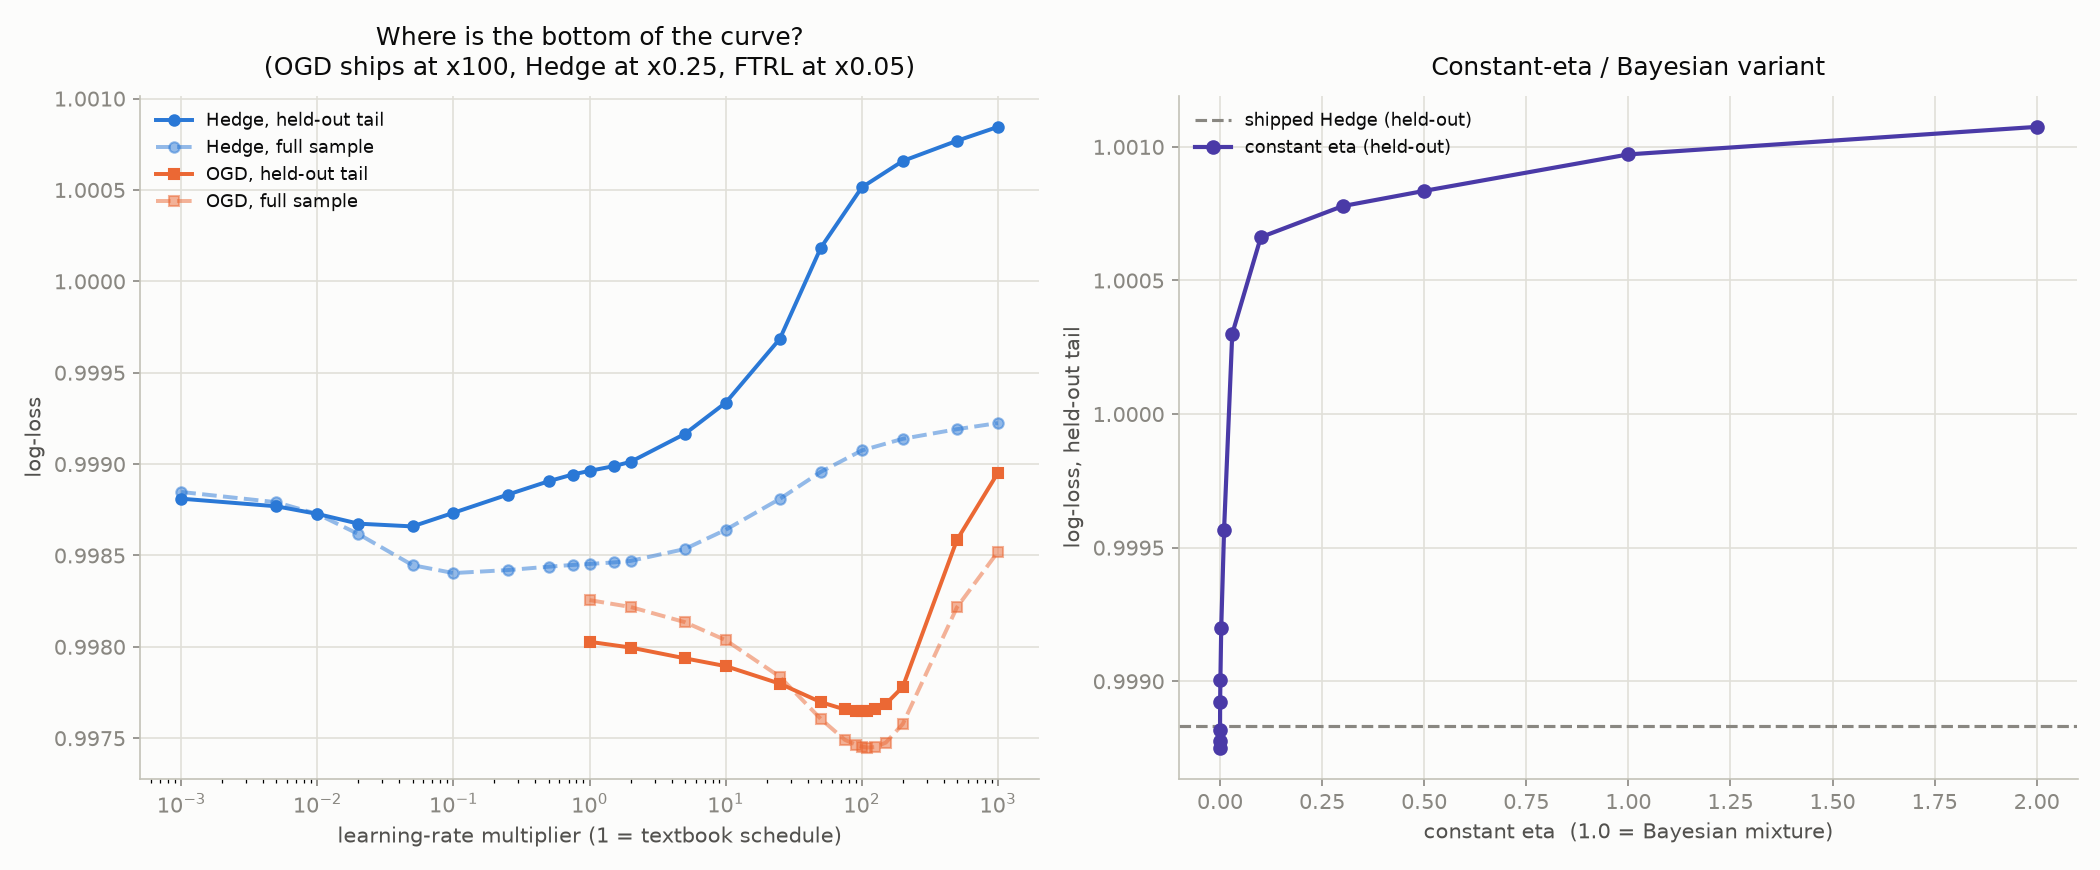
\includegraphics[width=0.92\linewidth]{learning_rate_study.png}
  \caption{Σάρωση του συντελεστή βήματος και για τους τρεις αλγορίθμους. Η επιλογή γίνεται στο χρονολογικό πρόθεμα· η ουρά αναφέρεται ως επαλήθευση. Το OGD παρουσιάζει γνήσιο εσωτερικό βέλτιστο. Οι καμπύλες ουράς των Hedge και FTRL συνεχίζουν να πέφτουν προς τα αριστερά, αλλά η επιλογή δεν γίνεται πάνω σε αυτές --- βλ.\ το σχόλιο για την επιφύλαξη που αποδείχθηκε ανυπόστατη.}
  \label{fig:lr}
\end{figure}

Το OGD θέλει βήμα εκατό φορές μεγαλύτερο από το θεωρητικό, με γνήσιο εσωτερικό βέλτιστο:
πλατό στο διάστημα $\times 75$ ως $\times 110$, με τα $\times 200$, $\times 500$ και
$\times 1000$ σαφώς χειρότερα. Τα Hedge και FTRL θέλουν βήμα \emph{μικρότερο}, κατά
παράγοντα 4 και 20 αντίστοιχα.

\paragraph{Μια επιφύλαξη που αποδείχθηκε ανυπόστατη.} Το ελάχιστο της \emph{ουράς} για τον
Hedge και τον FTRL βρίσκεται χαμηλότερα από τις τιμές που χρησιμοποιούνται, στο
$\times 0{,}05$ και $\times 0{,}005$ αντίστοιχα, και για ένα διάστημα η εργασία κουβαλούσε την
επιφύλαξη ότι οι δύο αυτοί αλγόριθμοι αναφέρονται με υποβέλτιστο βήμα. Η επιφύλαξη ήταν λάθος,
και ο λόγος αξίζει να ειπωθεί: \textbf{η επιλογή με βάση την ουρά είναι επιλογή πάνω στο
σύνολο ελέγχου}, δηλαδή ακριβώς ό,τι το πρωτόκολλο του \S\ref{sec:protocol} υπάρχει για να
αποτρέψει. Επειδή το log-loss είναι απλός μέσος όρος ανά γύρο, η τιμή του προθέματος ανακτάται
ακριβώς από το πλήρες δείγμα και την ουρά, ως
$(\text{πλήρες}\cdot T - \text{ουρά}\cdot n_{\text{ουράς}})/n_{\text{train}}$, και υπό το
πρωτόκολλο η απάντηση αντιστρέφεται: ο Hedge επιλέγει $\times 0{,}25$ και ο FTRL
$\times 0{,}05$, δηλαδή \emph{ακριβώς} τους ισχύοντες συντελεστές.

Τα νούμερα δείχνουν και γιατί. Στον Hedge το $\times 0{,}05$ δίνει train $0{,}99838$ έναντι
$0{,}99828$ του $\times 0{,}25$, και στον FTRL το $\times 0{,}005$ δίνει $0{,}99862$ έναντι
$0{,}99828$ του $\times 0{,}05$: και στις δύο περιπτώσεις η σειρά \emph{αντιστρέφεται} μεταξύ
προθέματος και ουράς, που είναι η υπογραφή της προσαρμογής στην ουρά και όχι ενδείξεις
καλύτερης ρύθμισης. Το OGD παραμένει βέλτιστο στο $\times 100$, με το $\times 110$ να δίνει
ταυτόσημη ουρά --- ισοπαλία μέσα στο ήδη περιγραφόμενο πλατό.

\paragraph{Σταθερό βήμα: η μία ιδέα χρονοδιαγράμματος που δεν είχε δοκιμαστεί σωστά.} Το
φθίνον $1/\sqrt{t}$ παράγεται για \emph{στατικό} comparator, ενώ το panel εδώ δεν είναι
στατικό, οπότε ένα βήμα που δεν σταματά ποτέ να κινείται είναι η θεωρητικά υποδεικνυόμενη
εναλλακτική. Είχε δοκιμαστεί μόνο για τον Hedge και μόνο στο διάστημα $[0{,}1, 2]$ --- ενώ το
ισχύον φθίνον βήμα του Hedge περνά από $\eta \approx 0{,}033$ στον πρώτο γύρο και
$\eta \approx 1{,}7\cdot10^{-4}$ στη μέση της περιόδου, δηλαδή ολόκληρη η ενδιαφέρουσα περιοχή
βρισκόταν \emph{κάτω} από το παλιό πλέγμα. Η σάρωση επεκτάθηκε σε πέντε δεκάδες και στους
τρεις αλγορίθμους, με επιλογή στο πρόθεμα και ζευγαρωμένο έλεγχο στην ουρά.

\begin{table}[H]
\centering
\begin{tabular}{@{}lrrrrl@{}}
\toprule
& \textbf{σταθερό $\eta$} & \textbf{ουρά} & \textbf{φθίνον} & \textbf{$p$} & \\
\midrule
Hedge & $3\cdot10^{-4}$ & 0,99892 & 0,99883 & $<0{,}001$ & φθίνον \\
OGD   & $0{,}1$         & 0,99795 & 0,99765 & $0{,}021$  & φθίνον \\
FTRL  & $10^{-5}$       & 0,99879 & 0,99889 & $0{,}001$  & \textbf{σταθερό} \\
\bottomrule
\end{tabular}
\caption{Σταθερό έναντι φθίνοντος βήματος. Το $\eta$ επιλέγεται στο χρονολογικό πρόθεμα και η
σύγκριση γίνεται στην ουρά με moving block bootstrap.}
\label{tab:const-step}
\end{table}

Το αποτέλεσμα είναι αρνητικό για τους δύο και \textbf{θετικό για τον έναν}. Στον Hedge και τον
OGD το σταθερό βήμα χάνει σημαντικά, κατά $+0{,}000089$ και $+0{,}000299$ αντίστοιχα. Στον
FTRL όμως κερδίζει σημαντικά, κατά $-0{,}000096$ ($p=0{,}001$) --- και το κρίσιμο είναι ότι τα
δύο σχήματα έχουν \emph{ταυτόσημο} score στο πρόθεμα ($0{,}99828$ και τα δύο): η επιλογή δεν
προτίμησε το σταθερό για να κολακεύσει την ουρά, το διάλεξε σε ισοπαλία και εκείνο κέρδισε
εκτός δείγματος. Η εξήγηση είναι η ίδια ασυμμετρία που εξηγεί και τις αντίθετες κατευθύνσεις
συντονισμού: το $\eta$ του FTRL πολλαπλασιάζει ολόκληρη τη σωρευμένη απώλεια, όχι την κλίση
ενός γύρου, οπότε είναι ο ένας από τους τρεις για τον οποίο «μη φθίνον» σημαίνει κάτι ποιοτικά
διαφορετικό.

Η σάρωση χρειάστηκε επέκταση και εδώ, για τον ίδιο λόγο όπως πριν: το ελάχιστο του FTRL
καθόταν αρχικά στο κάτω άκρο του πλέγματος. Επεκτεινόμενο ως το $10^{-9}$ έγινε γνήσια
εσωτερικό, και η επέκταση επιβεβαίωσε ταυτόχρονα το θεωρητικό όριο: για
$\eta \to 0$ ο FTRL εκφυλίζεται στον ομοιόμορφο μέσο, και πράγματι στο $\eta=10^{-9}$ δίνει
$0{,}99882$, την τιμή του ομοιόμορφου μέσου στην ουρά.

\paragraph{Ένα μεθοδολογικό σφάλμα που αξίζει να αναφερθεί.} Η αρχική σάρωση είχε πλέγμα
$1, 2, 5, \dots, 1000$ και κατέληξε ότι τα Hedge και FTRL είναι «ήδη βέλτιστα στο
$\times 1$». Το $1$ όμως ήταν το \emph{κάτω άκρο του πλέγματος}, όχι βέλτιστο, και κανείς
δεν είχε κοιτάξει αριστερά του. Η επέκταση προς τα κάτω αποκάλυψε γνήσια εσωτερικά ελάχιστα,
με κέρδος $+0{,}00013$ και $+0{,}00018$ αντίστοιχα στην ουρά. Το συμπέρασμα γενικεύεται: όταν
η απάντηση μιας σάρωσης βρίσκεται στο άκρο του πλέγματος, το πλέγμα πρέπει να επεκταθεί πριν
θεωρηθεί απάντηση.

Η αντίθετη κατεύθυνση έχει δομική εξήγηση. Το $\eta$ του OGD πολλαπλασιάζει την κλίση
\emph{ενός} γύρου, οπότε η αύξησή του σημαίνει μεγαλύτερη μετακίνηση. Το $\eta$ του Hedge
βρίσκεται σε εκθέτη πάνω στην απώλεια ενός γύρου, οπότε η μείωσή του \emph{μακραίνει τη
μνήμη}. Το $\eta$ του FTRL πολλαπλασιάζει ολόκληρη τη σωρευμένη απώλεια, οπότε η αύξησή του
τον καταρρέει προς follow-the-leader.

\section{Κατάταξη στο πλήρες panel}

\begin{table}[H]
\centering
\small
\begin{tabular}{@{}lllrr@{}}
\toprule
& & \textbf{φάση} & \textbf{log-loss} & \textbf{Brier} \\
& & & (raw / cal.) & (raw / cal.) \\
\midrule
PSC (Pinnacle) & bookmaker  & closing & 0,99714 / 0,99685 & 0,59592 / 0,59577 \\
OGD            & αλγόριθμος & ---     & 0,99745 / 0,99693 & 0,59612 / 0,59586 \\
Hedge          & αλγόριθμος & ---     & 0,99842 / 0,99773 & 0,59674 / 0,59637 \\
FTRL           & αλγόριθμος & ---     & 0,99843 / 0,99774 & 0,59674 / 0,59638 \\
Uniform        & baseline   & ---     & 0,99886 / 0,99813 & 0,59703 / 0,59665 \\
VC\_BV         & bookmaker  & opening & 1,00075 / 1,00026 & 0,59833 / 0,59806 \\
WH             & bookmaker  & opening & 1,00119 / 1,00048 & 0,59860 / 0,59818 \\
PS (Pinnacle)  & bookmaker  & opening & 1,00083 / 1,00055 & 0,59838 / 0,59824 \\
IW             & bookmaker  & opening & 1,00186 / 1,00061 & 0,59899 / 0,59826 \\
BW             & bookmaker  & opening & 1,00140 / 1,00065 & 0,59873 / 0,59833 \\
B365           & bookmaker  & opening & 1,00113 / 1,00073 & 0,59852 / 0,59832 \\
\bottomrule
\end{tabular}
\caption{Κατάταξη κατά βαθμονομημένο log-loss, bookmakers με κάλυψη $\geq$70\%.}
\label{tab:ranking}
\end{table}

\begin{figure}[htbp]
  \centering
  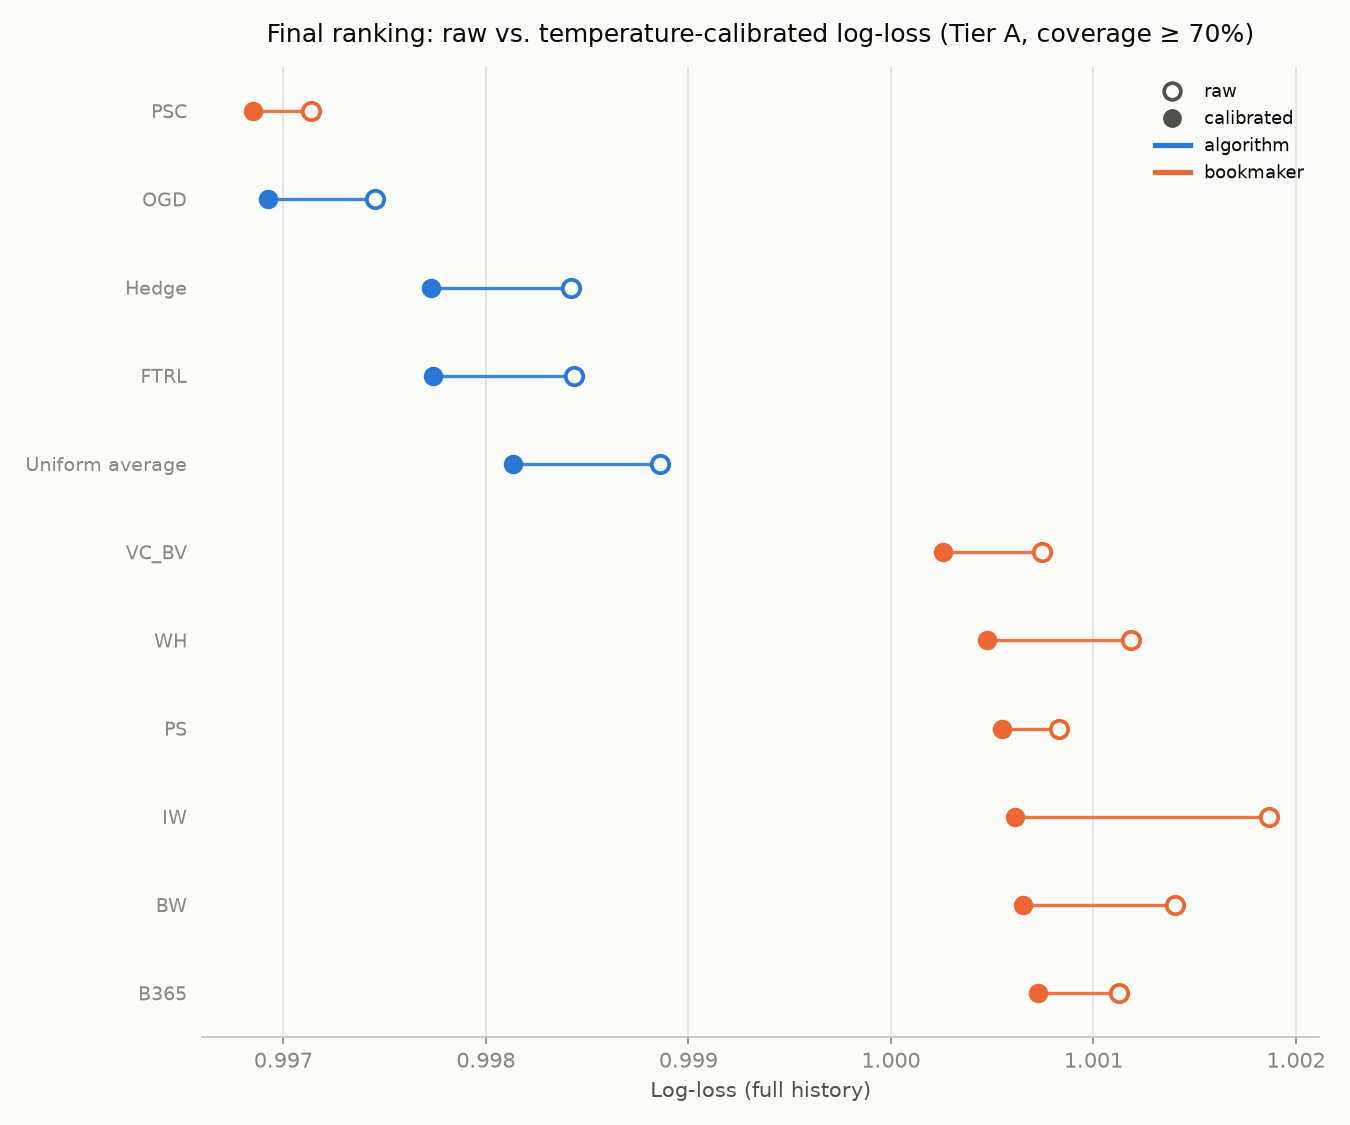
\includegraphics[width=0.92\linewidth]{final_ranking.png}
  \caption{Κάθε σειρά: κενός κύκλος το raw log-loss, γεμάτος το βαθμονομημένο. Η επιλογή dot/slope plot αντί ραβδογράμματος είναι σκόπιμη, καθώς τα log-loss συγκεντρώνονται γύρω από το $1{,}0$ χωρίς ουσιαστικό μηδέν και ένα ραβδόγραμμα με κομμένο άξονα θα μεγεθύνε οπτικά μικροσκοπικές διαφορές.}
  \label{fig:ranking}
\end{figure}

Τα ζευγαρωτά τεστ δίνουν:

\begin{itemize}
  \item Και οι τρεις αλγόριθμοι ξεπερνούν σημαντικά την ομοιόμορφη μέση τιμή: OGD
        $-0{,}00141$, Hedge $-0{,}00044$, FTRL $-0{,}00043$, όλα $p<0{,}001$. Το περιθώριο
        του OGD είναι περίπου τριπλάσιο.
  \item Το OGD ξεπερνά σημαντικά τους Hedge ($-0{,}00097$), FTRL ($-0{,}00098$) και
        B365C ($-0{,}00063$).
  \item Η βαθμονόμηση βελτιώνει σημαντικά και τις τέσσερις μεθόδους, κατά $+0{,}00053$ έως
        $+0{,}00073$.
  \item Ο PSC παραμένει σημαντικά μπροστά από το OGD σε αυτή τη διαμόρφωση: $+0{,}00043$
        βαθμονομημένο, $p<0{,}001$, στους 71.818 κοινούς αγώνες.
\end{itemize}

\paragraph{Μια αναγκαία επιφύλαξη.} Το κατώφλι κάλυψης 70\% αφήνει μέσα έναν μόνο closing
bookmaker, τον PSC, επειδή οι υπόλοιπες closing στήλες αρχίζουν γύρω στο 2019/20 και ο B365C
χάνει οριακά με 69,6\%. Η διατύπωση «ξεπερνάμε όλους εκτός του PSC» σημαίνει επομένως,
\emph{εδώ}, ότι ξεπερνάμε έξι τιμές ανοίγματος. Η ουσιαστική σύγκριση απέναντι σε τιμές
κλεισίματος γίνεται στις \S\ref{sec:res-recent} και \S\ref{sec:res-deploy}.

Σημειώνεται ότι η Interwetten καταλαμβάνει την
\emph{τελευταία} θέση της κατάταξης σε raw log-loss ($1{,}00186$) παρότι έχει την έβδομη
καλύτερη κάλυψη. Η προσθήκη της κάνει επομένως τη διατύπωση «ξεπερνάμε όλους εκτός του PSC»
κάπως ευκολότερη, και γι' αυτό η ουσιαστική σύγκριση παραμένει αυτή απέναντι στους PSC και
B365C.

Σημειώνεται επίσης ότι το log-loss και το Brier δίνουν σχεδόν ταυτόσημη σειρά, με μόνη
εξαίρεση τις δύο τελευταίες θέσεις. Η accuracy δίνει άλλη σειρά, αλλά καμία διαφορά της δεν
είναι στατιστικά σημαντική --- αναμενόμενο, αφού δεν είναι κατάλληλος κανόνας βαθμολόγησης.

\section{Ποιο panel}
\label{sec:res-panels}

\begin{table}[H]
\centering
\small
\begin{tabular}{@{}lrrrrrr@{}}
\toprule
& \multicolumn{2}{c}{\textbf{opening} (13)} & \multicolumn{2}{c}{\textbf{όλα} (26)} & \multicolumn{2}{c}{\textbf{closing} (13)} \\
\cmidrule(lr){2-3}\cmidrule(lr){4-5}\cmidrule(lr){6-7}
& απλή & Shin & απλή & Shin & απλή & Shin \\
\midrule
OGD     & 1,00076 & 1,00024 & 0,99745 & 0,99709 & 0,99722 & 0,99689 \\
Hedge   & 1,00088 & 1,00033 & 0,99842 & 0,99781 & 0,99762 & 0,99714 \\
FTRL    & 1,00088 & 1,00033 & 0,99843 & 0,99782 & 0,99761 & 0,99714 \\
Uniform & 1,00080 & 1,00022 & 0,99886 & 0,99824 & 0,99748 & 0,99703 \\
\bottomrule
\end{tabular}
\caption{Log-loss ανά panel και μέθοδο de-vig.}
\end{table}

\begin{figure}[htbp]
  \centering
  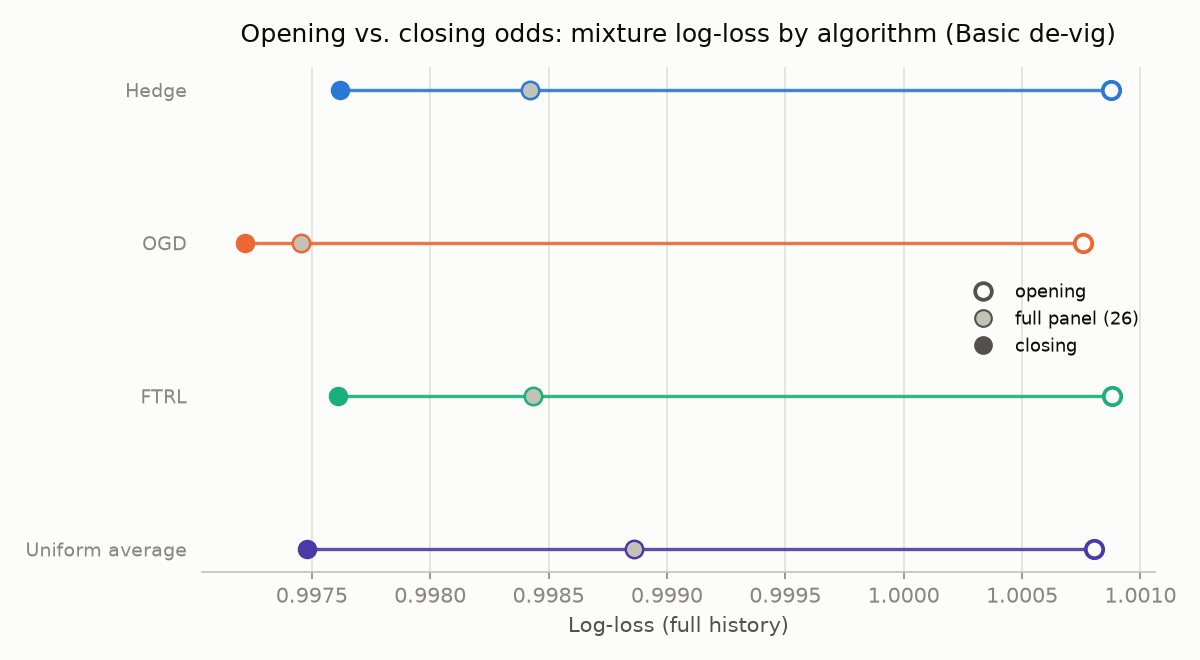
\includegraphics[width=0.92\linewidth]{opening_vs_closing.png}
  \caption{Σύγκριση των τριών panel για κάθε αλγόριθμο. Η διάταξη closing $<$ όλα $<$ opening ισχύει σε κάθε περίπτωση.}
  \label{fig:panels}
\end{figure}

Η διάταξη closing $<$ όλα $<$ opening ισχύει σε κάθε κελί, και στις 24 συγκρίσεις (4
αλγόριθμοι $\times$ 3 συγκρίσεις $\times$ 2 κανονικοποιήσεις) η διαφορά είναι στατιστικά
σημαντική. Ότι οι τιμές κλεισίματος υπερέχουν των ανοιγμάτων είναι αναμενόμενο. Το μη
αναμενόμενο είναι ότι το closing-only panel ξεπερνά και το \emph{πλήρες}: οι opening
bookmakers δεν λειτουργούν ως χρήσιμη διαφοροποίηση αλλά ως καθαρό βάρος στο μείγμα.

Η σύγκριση κάθε αλγορίθμου με τον απλό μέσο όρο \emph{μέσα} στο ίδιο panel εξηγεί τον
μηχανισμό και αποτελεί, κατά τη γνώμη μας, το γενικότερα χρησιμότερο εύρημα της εργασίας:

\begin{itemize}
  \item Στο \textbf{πλήρες} panel και οι τρεις αλγόριθμοι κερδίζουν σημαντικά τον μέσο όρο.
  \item Στα \textbf{περιορισμένα} panel οι Hedge και FTRL \emph{χάνουν σημαντικά} από τον
        μέσο όρο, σε 8 από 8 τεστ. Το OGD κερδίζει στο closing και ισοπαλεί στο opening.
\end{itemize}

Το πλήρες panel περιέχει 13 καλούς closing και 13 συστηματικά χειρότερους opening experts,
δηλαδή σαφή ποιοτική διαφορά προς εκμάθηση. Σε ομοιογενές panel η διαφορά αυτή λείπει, και
για δύο από τους τρεις αλγορίθμους η προσαρμογή κοστίζει περισσότερο απ' όσο αποδίδει.

\section{Πού ακριβώς υπερέχουν οι τιμές κλεισίματος}
\label{sec:res-arrival}

Η προηγούμενη ενότητα δείχνει ότι το closing panel κερδίζει κατά $\sim0{,}0035$ σε log-loss.
Αυτό είναι μέσος όρος, και η Παρατήρηση~\ref{rem:closing} κάνει αυστηρότερη πρόβλεψη: αν η
υπεροχή οφείλεται στην άφιξη πληροφορίας, πρέπει να συγκεντρώνεται εκεί όπου η τιμή
\emph{όντως κινήθηκε}. Για να ελεγχθεί, κάθε αγώνας χαρακτηρίζεται από την απόσταση ολικής
μεταβολής ανάμεσα στην αρχική και την τελική πιθανοτική κατανομή κάθε οίκου, μέσο όρο πάνω
στα 13 διαθέσιμα ζεύγη opening/closing, και οι αγώνες χωρίζονται σε πεμπτημόρια.

\begin{table}[H]
\centering
\small
\begin{tabular}{@{}lrrrrr@{}}
\toprule
\textbf{Πεμπτημόριο κίνησης} & Q1 & Q2 & Q3 & Q4 & Q5 \\
\midrule
Μέση κίνηση & 0,0082 & 0,0144 & 0,0215 & 0,0324 & 0,0598 \\
log-loss opening & 0,99161 & 1,00581 & 1,00068 & 1,00666 & 1,00790 \\
log-loss closing & 0,99118 & 1,00509 & 0,99868 & 1,00214 & 0,99632 \\
\midrule
\textbf{closing $-$ opening} & $-0{,}00044$ & $-0{,}00072$ & $-0{,}00200$ & $-0{,}00452$ &
$\mathbf{-0{,}01158}$ \\
$p$ & 0,052 & 0,050 & $<0{,}001$ & $<0{,}001$ & $<0{,}001$ \\
\bottomrule
\end{tabular}
\caption{Πλεονέκτημα κλεισίματος ανά πεμπτημόριο κίνησης της γραμμής, 10.649--10.650 αγώνες
ανά πεμπτημόριο.}
\label{tab:arrival}
\end{table}

\begin{figure}[H]
\centering
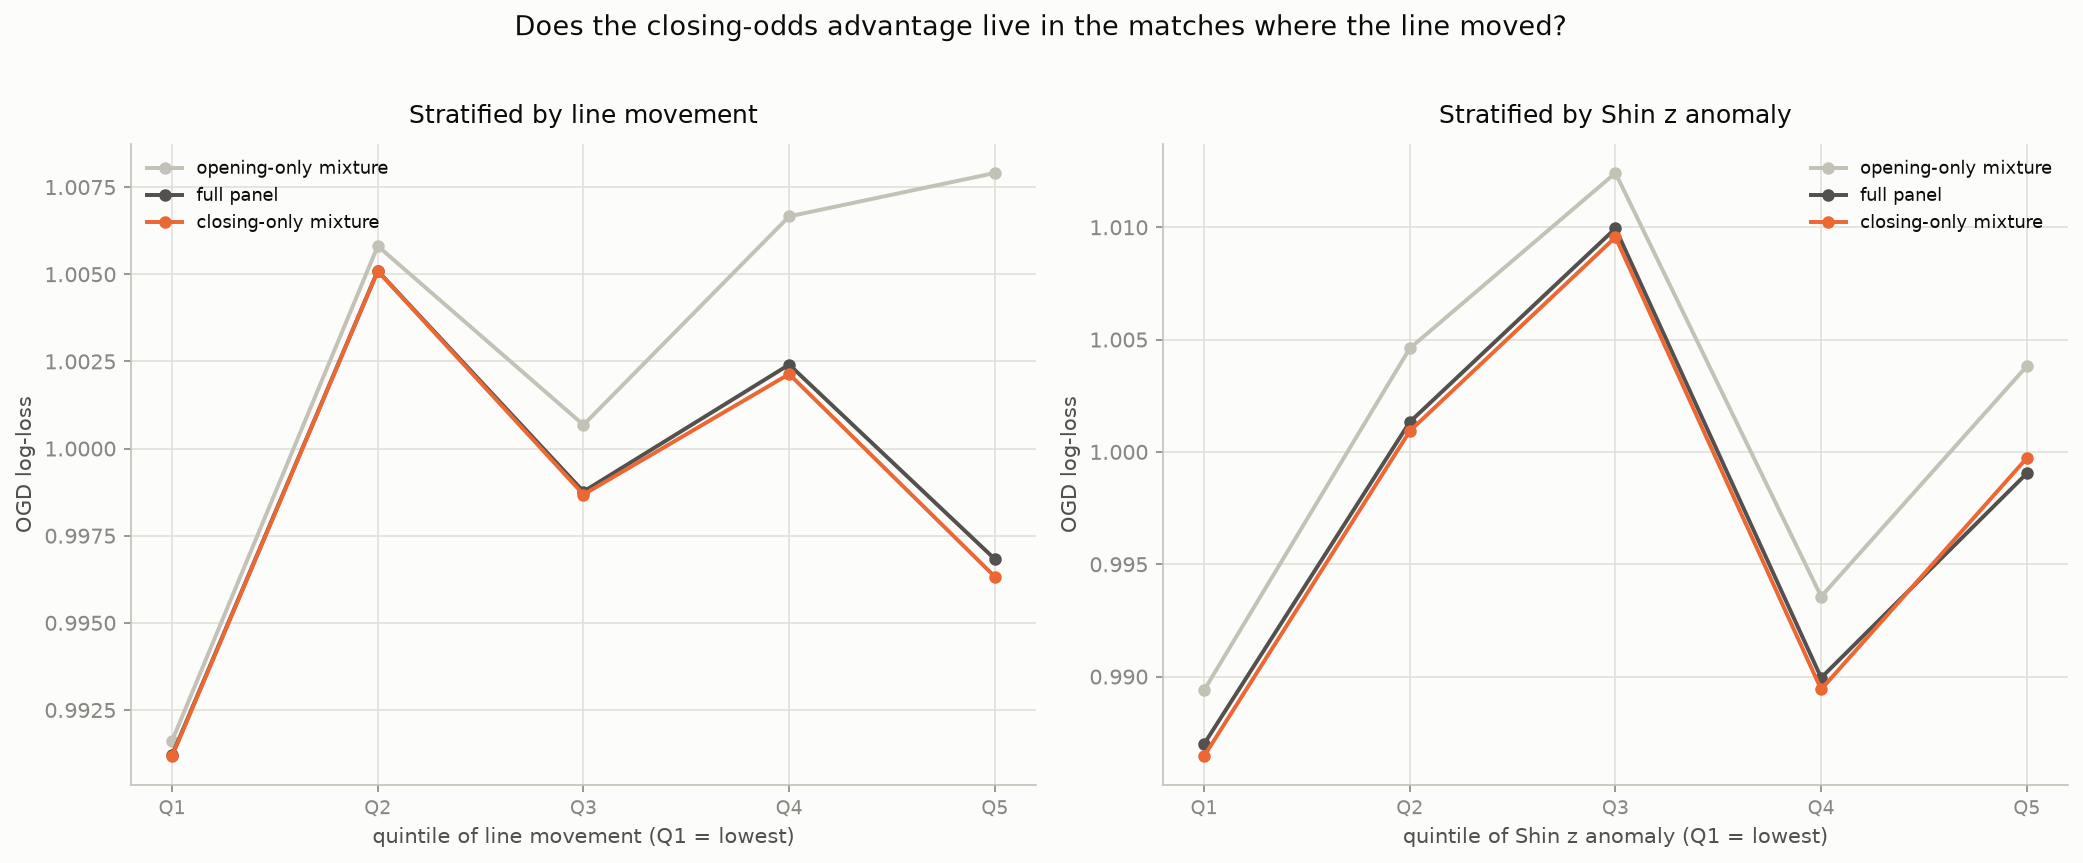
\includegraphics[width=\textwidth]{information_arrival.png}
\caption{Αριστερά η στρωμάτωση κατά κίνηση της γραμμής, δεξιά κατά ανωμαλία του $z$ του Shin.}
\end{figure}

\paragraph{Η πρόβλεψη επιβεβαιώνεται, με διαβάθμιση 26 φορών.} Το πλεονέκτημα του κλεισίματος
πηγαίνει από $-0{,}00044$ στο ήσυχο πέμπτο των αγώνων σε $-0{,}01158$ στο θορυβώδες. Στο Q1
μάλιστα \textbf{δεν είναι καν στατιστικά σημαντικό} ($p=0{,}052$): στο ένα πέμπτο των αγώνων
όπου η γραμμή σχεδόν δεν κινήθηκε, δεν υπάρχει μετρήσιμο πλεονέκτημα κλεισίματος. Η «υπεροχή
των τιμών κλεισίματος» δεν είναι επομένως γενική ιδιότητα των τελικών τιμών αλλά φαινόμενο
του άνω πεμπτημορίου.

\paragraph{Μια αναγκαία επιφύλαξη.} Η κίνηση μετριέται από τις \emph{ίδιες} τιμές κλεισίματος
που χρησιμοποιεί το closing panel, οπότε το μηδενικό αποτέλεσμα του Q1 είναι εν μέρει
μηχανικό: αν οι δύο τιμές σχεδόν ταυτίζονται, τα δύο μείγματα δεν μπορούν να διαφέρουν πολύ.
Το μη τετριμμένο σκέλος είναι η \emph{κατεύθυνση} στο άλλο άκρο. Μια μεγάλη κίνηση θα
μπορούσε κάλλιστα να πηγαίνει προς τη λάθος μεριά· το ότι η μεταγενέστερη τιμή είναι
συστηματικά η καλύτερη κατά $0{,}0116$ είναι ακριβώς ο ισχυρισμός αποδοτικότητας της αγοράς,
εντοπισμένος εκεί όπου πράγματι λειτουργεί. Χρήσιμος έλεγχος: η \emph{δυσκολία} των αγώνων
δεν είναι μονότονη στα πεμπτημόρια (το log-loss του πλήρους panel πηγαίνει $0{,}99120$,
$1{,}00510$, $0{,}99877$, $1{,}00241$, $0{,}99683$), ενώ το πλεονέκτημα είναι, οπότε η
διαβάθμιση δεν είναι τεχνούργημα του τύπου «δυσκολότεροι αγώνες, μεγαλύτερες διαφορές».

\paragraph{Το $z$ του Shin είναι πολύ ασθενέστερος δείκτης.} Στρωματώνοντας αντ' αυτού κατά
την ανωμαλία του $z$ --- ποσότητα που το \S\ref{sec:microstructure-theory} ταυτίζει με την
εκτιμώμενη αναλογία πληροφορημένων --- η διαβάθμιση είναι μόλις $-0{,}00295$ έως
$-0{,}00498$, δηλαδή παράγοντας $1{,}7$ έναντι $26$, με όλα τα πεμπτημόρια σημαντικά. Το $z$
δηλαδή ανιχνεύει κάτι, αλλά η πραγματική κίνηση της τιμής είναι ασύγκριτα καθαρότερος
δείκτης του ότι έφτασε πληροφορία --- εύλογο, αφού το $z$ εκτιμάται από μία στιγμή της
αγοράς ενώ η κίνηση παρατηρεί τη διαφορά δύο.

\section{Η διαμόρφωση που επιλέγεται}
\label{sec:res-config}

Τρεις βελτιώσεις είχαν μετρηθεί χωριστά --- το διορθωμένο βήμα, το closing-only panel, το
Shin --- και συνδυάζονται εδώ. Κάθε διαμόρφωση βαθμολογείται στους ίδιους 71.818 αγώνες, την
τομή όλων με τον PSC, σύμφωνα με την αρχή του \S\ref{sec:common-rounds}.

\begin{table}[H]
\centering
\begin{tabular}{@{}lrrr@{}}
\toprule
\textbf{Διαμόρφωση} & \textbf{πλήρες} & \textbf{train} & \textbf{ουρά 25\%} \\
\midrule
PSC μόνος του                     & 0,99685 & 0,99746 & 0,99502 \\
closing-only $+$ Shin             & 0,99692 & 0,99754 & 0,99507 \\
closing-only, αναλογική           & 0,99693 & 0,99756 & 0,99506 \\
closing-only $+$ Shin, χωρίς μονής σεζόν & 0,99692 & 0,99754 & 0,99509 \\
πλήρες panel, αναλογική           & 0,99728 & 0,99801 & 0,99508 \\
πλήρες panel, Shin                & 0,99731 & 0,99804 & 0,99512 \\
\bottomrule
\end{tabular}
\caption{Βαθμονομημένο log-loss του OGD ανά διαμόρφωση, ίδιοι 71.818 αγώνες παντού.}
\end{table}

\begin{figure}[htbp]
  \centering
  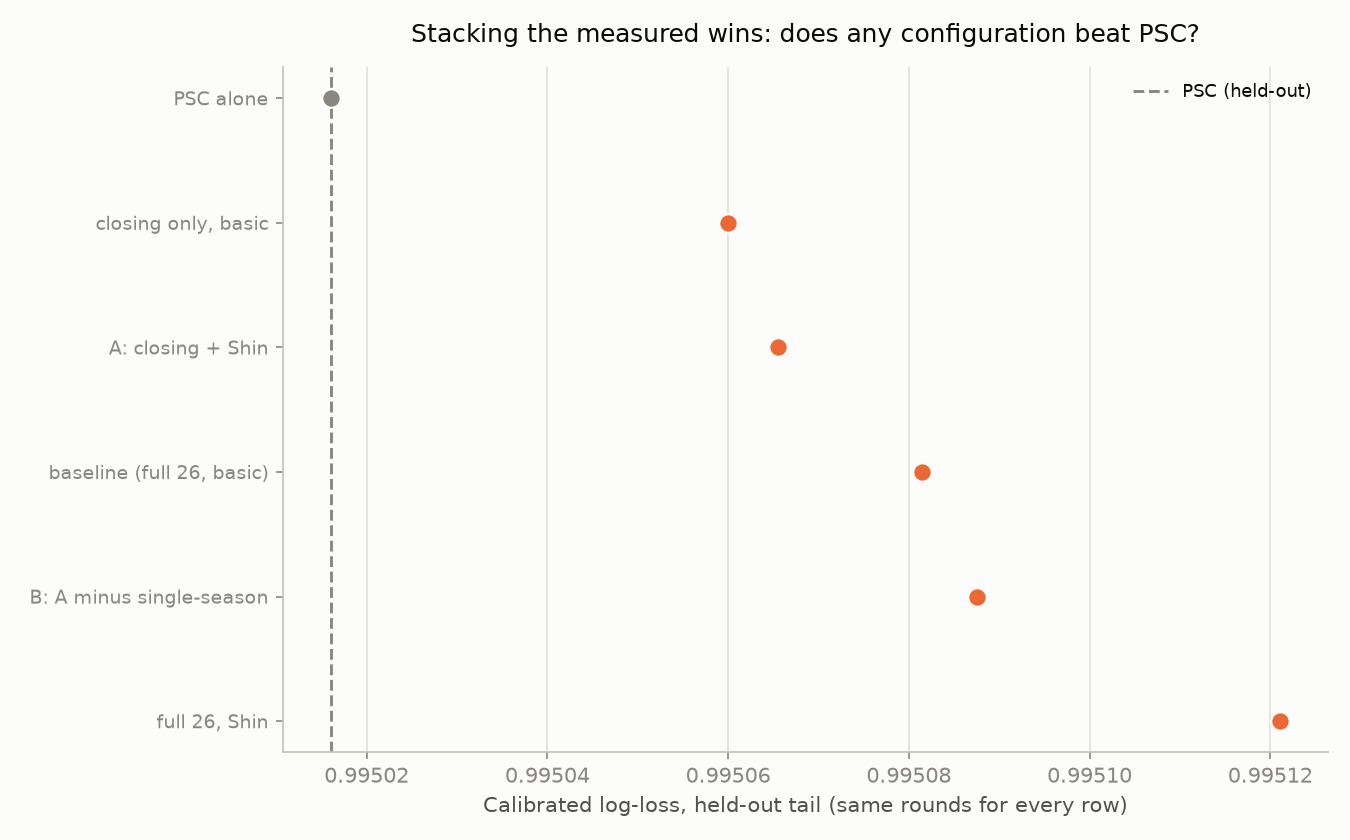
\includegraphics[width=0.92\linewidth]{best_configuration.png}
  \caption{Οι διαμορφώσεις στην ουρά ελέγχου, με τον PSC ως γραμμή αναφοράς. Όλες συγκεντρώνονται εντός $0{,}00005$.}
  \label{fig:bestconfig}
\end{figure}

\begin{itemize}
  \item \textbf{Το panel κάνει όλη τη δουλειά.} Η closing-only $+$ Shin ξεπερνά το πλήρες
        panel κατά $-0{,}00036$ ($p<0{,}001$), και η closing-only με αναλογική
        κανονικοποίηση κατά $-0{,}00034$ ($p<0{,}001$).
  \item \textbf{Το Shin μόνο του δεν προσφέρει τίποτα μετρήσιμο} πάνω στο πλήρες panel
        ($+0{,}00004$, $p=0{,}181$) --- συνεπές με το ότι Shin και temperature scaling
        διορθώνουν το ίδιο favorite-longshot bias, οπότε το δεύτερο απορροφά το πρώτο.
  \item \textbf{Έναντι του PSC}: το πλήρες panel χάνει σημαντικά ($+0{,}00043$,
        $p<0{,}001$), ενώ η closing-only $+$ Shin \emph{ισοπαλεί} ($+0{,}00007$,
        $p=0{,}234$) και η closing-only με αναλογική επίσης ($+0{,}00009$, $p=0{,}143$).
\end{itemize}

Η ουρά 25\% δεν αναδεικνύει νικητή: και οι έξι γραμμές μαζεύονται σε λιγότερο από
$0{,}00005$. Επιβεβαιώνει δηλαδή την ισοπαλία, και δεν θα ήταν έντιμο να παρουσιαστεί ως
νίκη. Σημειώνεται επίσης ότι σε κάθε closing διαμόρφωση ο PSC βρίσκεται \emph{μέσα} στο
μείγμα: το «φτάνουμε τον PSC» διαβάζεται «το μείγμα φτάνει το καλύτερο μέλος του».

\section{Χωρίς την Pinnacle}
\label{sec:res-nopinnacle}

Το προφανές αντεπιχείρημα είναι ότι το μείγμα απλώς αναπαράγει την Pinnacle, που ούτως ή
άλλως βρίσκεται μέσα του. Αφαιρώντας και τις δύο στήλες της και επανεκπαιδεύοντας από την
αρχή σε τρία panel:

\begin{table}[H]
\centering
\small
\begin{tabular}{@{}llrll@{}}
\toprule
\textbf{Panel} & \textbf{Θέση OGD} & \textbf{log-loss} & \textbf{Πρώτος} & \textbf{Ζευγαρωτά} \\
\midrule
πλήρες (24)      & \#3 από 9 & 0,99782 & FTRL 0,99771    & 5 νίκες, 0 ήττες \\
closing-only (12)& \#1 από 9 & 0,99919 & OGD (ο ίδιος)   & 3 νίκες, 2 ισοπαλίες \\
opening-only (12)& \#5 από 9 & 0,99999 & VC\_BV 0,99987 & 3 νίκες, \textbf{1 ήττα}, 1 ισοπαλία \\
\bottomrule
\end{tabular}
\caption{Κάθε panel επανεκπαιδεύεται από την αρχή και συγκρίνεται με τους bookmakers της
δικής του φάσης.}
\end{table}

\begin{figure}[htbp]
  \centering
  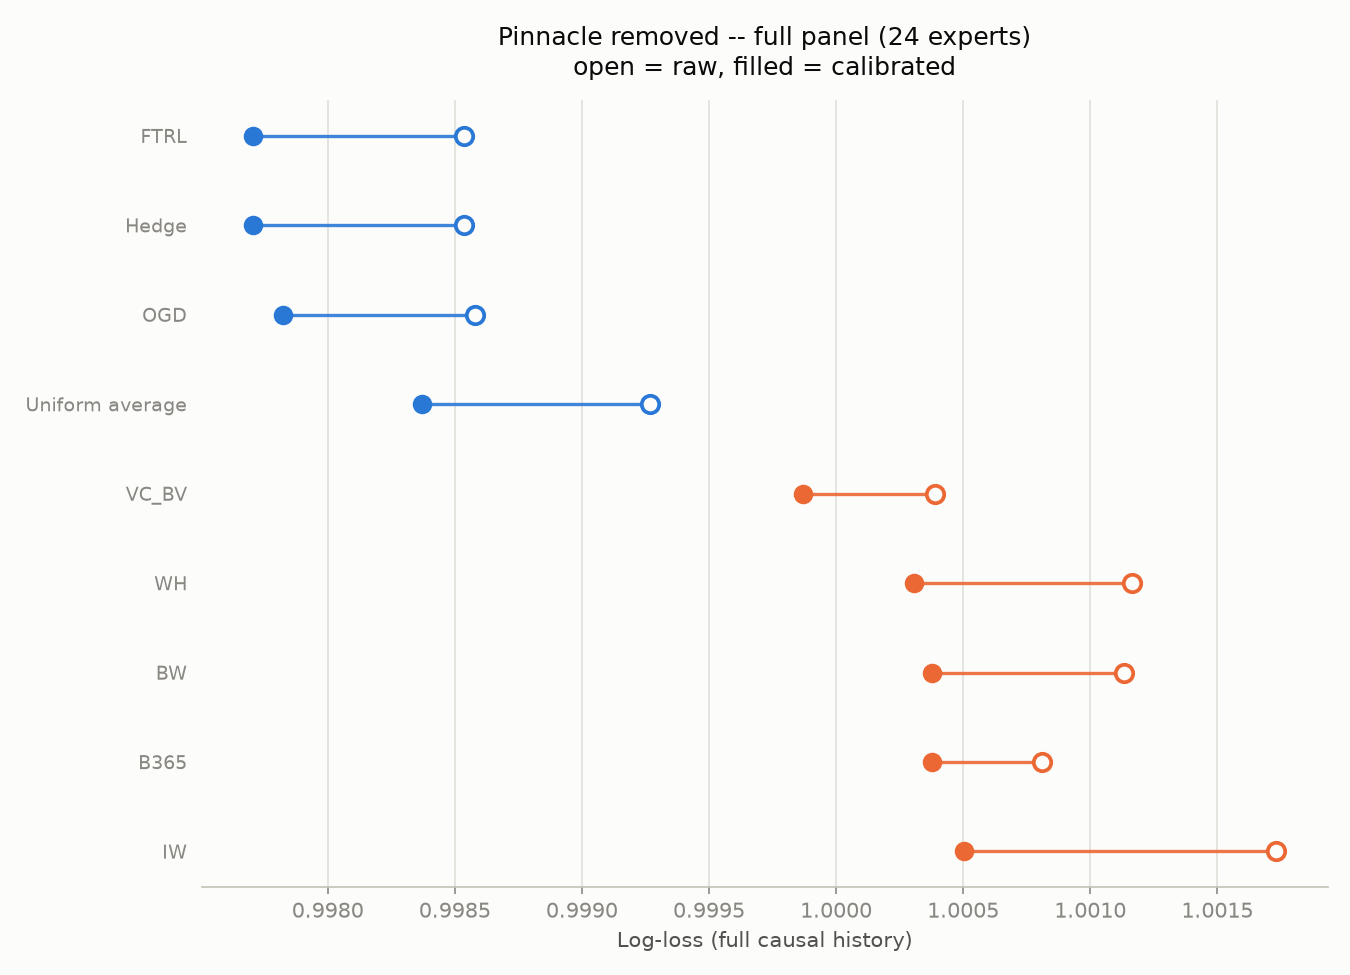
\includegraphics[width=0.92\linewidth]{no_pinnacle.png}
  \caption{Πλήρες panel χωρίς καμία στήλη Pinnacle. Και οι τέσσερις μέθοδοι βρίσκονται πάνω από όλους τους εναπομείναντες bookmakers.}
  \label{fig:nopinn}
\end{figure}

Στο \textbf{πλήρες} panel το αποτέλεσμα αντέχει άνετα: και οι τέσσερις μέθοδοι βρίσκονται
πάνω από όλους τους bookmakers, και το OGD κερδίζει σημαντικά και τους \emph{πέντε}, με
περιθώρια $-0{,}00181$ (VC\_BV) έως $-0{,}00315$ (IW) και $p<0{,}001$ παντού. Όλοι τους όμως
είναι opening.

Στα δύο \textbf{ομοιογενή} panel το αποτέλεσμα αλλάζει. Στο closing το OGD κερδίζει τρεις
(WHC $-0{,}00088$, IWC $-0{,}00077$, BWC $-0{,}00051$) και ισοπαλεί με τους B365C
($p=0{,}505$) και VC\_BVC ($p=0{,}284$)· κατατάσσεται μεν πρώτο, αλλά με τον απλό μέσο όρο
δεύτερο σε απόσταση $0{,}00002$, δηλαδή πρακτικά αδιάκριτο. Στο opening κερδίζει πάλι τρεις,
ισοπαλεί με τον B365 ($p=0{,}203$), αλλά \textbf{χάνει σημαντικά από τον VC\_BV}
($+0{,}00030$, $p=0{,}004$) --- η μόνη περίπτωση σε όλη την εργασία όπου μας ξεπερνά
σημαντικά \emph{bookmaker} εκτός της Pinnacle, και εκεί ο απλός μέσος όρος περνάει μπροστά
από το OGD. Η διατύπωση περιορίζεται σκόπιμα στους bookmakers: στον έλεγχο ανάπτυξης
(\S\ref{sec:res-deploy}) μας ξεπερνά σημαντικά και το Betfair Exchange, που όμως δεν είναι
bookmaker αλλά ανταλλακτήριο.

Το μοτίβο είναι αρκετά σταθερό ώστε να μην αποδοθεί στην τύχη, και επαναλαμβάνει το εύρημα
του \S\ref{sec:res-panels}: μόλις φύγει η Pinnacle, οι υπόλοιποι της ίδιας φάσης μοιάζουν
τόσο πολύ μεταξύ τους που δεν απομένει ποιοτική διαφορά προς εκμάθηση. Η διαμόρφωση που
επιλέγεται είναι λοιπόν η καλύτερη εν μέρει \emph{επειδή} περιέχει τον καλύτερο odds-setter
της αγοράς.

\section{Πρόσφατο παράθυρο}
\label{sec:res-recent}

Το κατώφλι κάλυψης ορίζεται από τη δεκαετία, γεγονός που ευνοεί όποιον έδινε αποδόσεις παλιά.
Περιορίζοντας στις τελευταίες πέντε σεζόν (38.749 αγώνες), οι B365C, BWC, VC\_BVC και WHC
περνούν όλοι το κατώφλι και η απαιτητική σύγκριση γίνεται δυνατή.

\begin{table}[H]
\centering
\small
\begin{tabular}{@{}rllr@{}}
\toprule
\textbf{\#} & \textbf{Σειρά} & \textbf{φάση} & \textbf{log-loss} \\
\midrule
1 & PSC & closing & 0,99439 \\
2 & \textbf{OGD} & --- & \textbf{0,99495} \\
3 & VC\_BVC & closing & 0,99498 \\
4 & WHC & closing & 0,99502 \\
5 & BWC & closing & 0,99504 \\
6 & B365C & closing & 0,99543 \\
7 & Uniform & --- & 0,99591 \\
8 & Hedge & --- & 0,99604 \\
9 & FTRL & --- & 0,99607 \\
10--14 & WH, PS, VC\_BV, BW, B365 & opening & 0,99771 και κάτω \\
\bottomrule
\end{tabular}
\caption{Τελευταίες πέντε σεζόν, πλήρες panel, βαθμονομημένο log-loss.}
\end{table}

\begin{figure}[htbp]
  \centering
  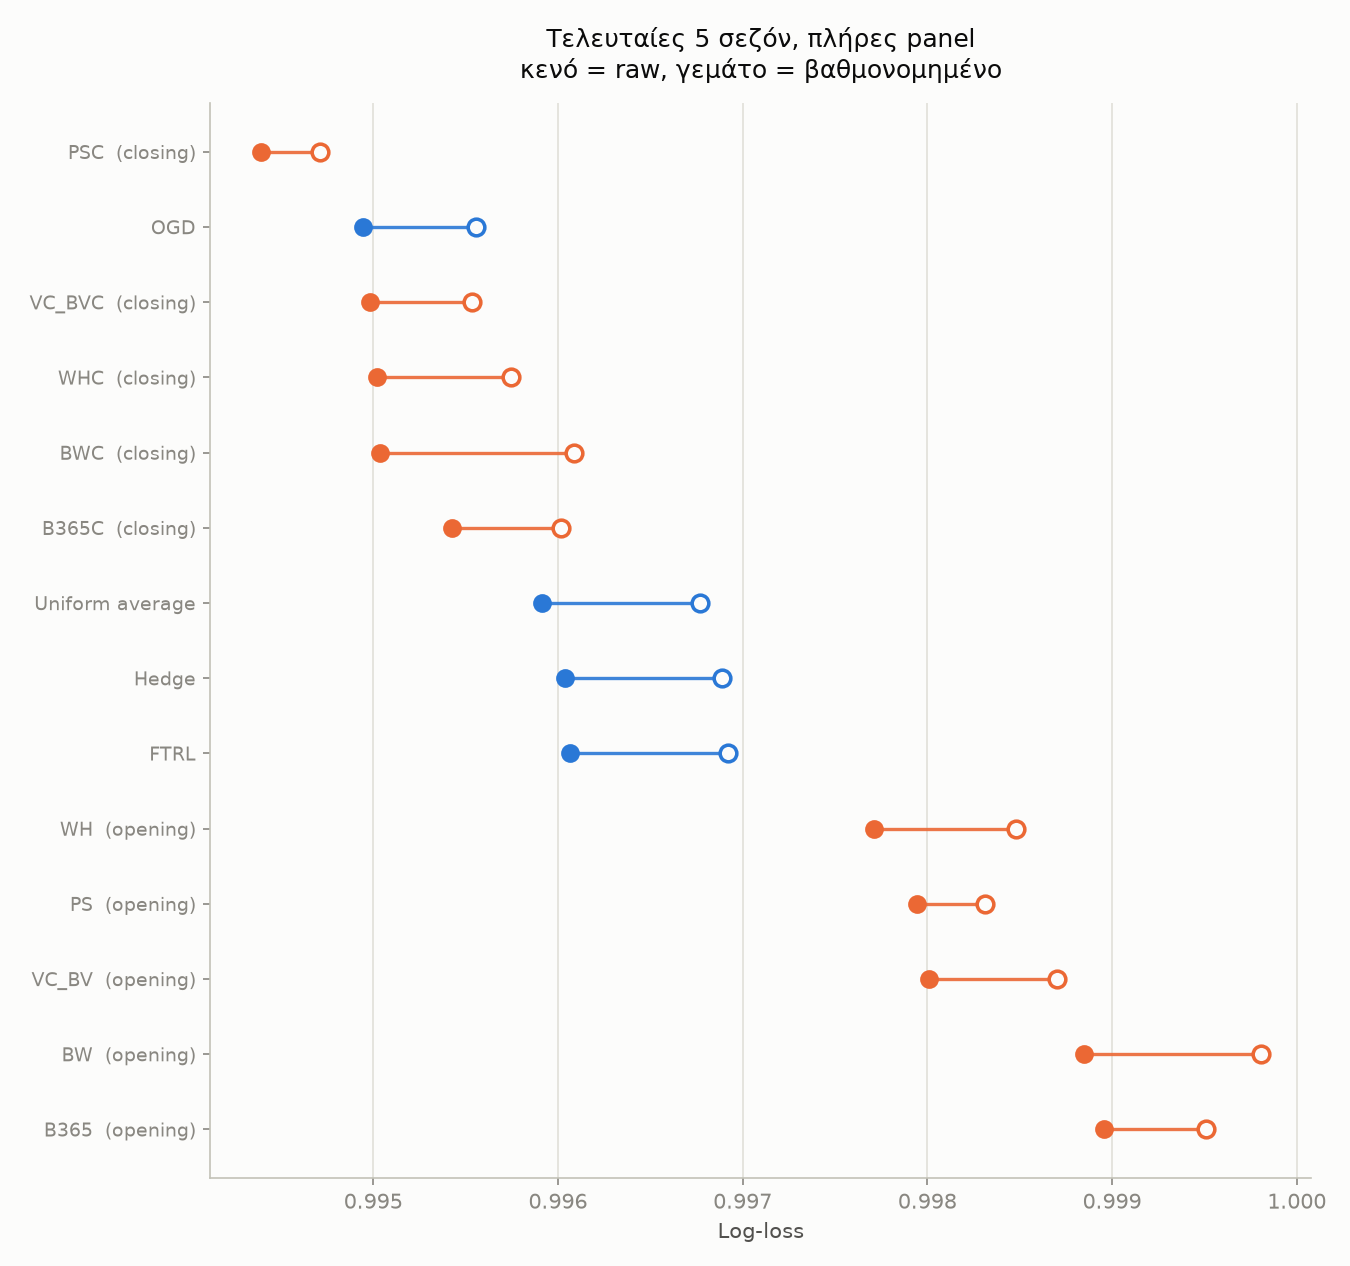
\includegraphics[width=0.92\linewidth]{recent_window.png}
  \caption{Τελευταίες πέντε σεζόν. Οι closing bookmakers περνούν πλέον το κατώφλι κάλυψης και η σύγκριση γίνεται απαιτητικότερη.}
  \label{fig:recent}
\end{figure}

Το OGD βρίσκεται στη θέση \#2, μπροστά από κάθε closing bookmaker πλην της Pinnacle, και η
διαφορά από τον PSC συρρικνώνεται σε $+0{,}00036$ ($p=0{,}014$) από $+0{,}00043$ της
δεκαετίας. Δύο ευρήματα όμως \emph{αντιστρέφονται} και αναφέρονται ρητά: οι Hedge και FTRL
χάνουν από τον απλό μέσο όρο σε \emph{όλα} τα panel εδώ, όχι μόνο στα περιορισμένα
($+0{,}00012$ και $+0{,}00015$, $p=0{,}006$ και $p=0{,}002$), και το log-loss με το Brier
παύουν να συμφωνούν στη σειρά.

\section{Έλεγχος ανάπτυξης}
\label{sec:res-deploy}

Ο έλεγχος με πραγματική χρονική τομή: προσαρμογή σε 65.009 γύρους ως 31/12/2024, μέτρηση σε
11.574 γύρους του 2025--26, από τους οποίους 8.151 κοινοί.

\begin{table}[H]
\centering
\small
\begin{tabular}{@{}rllr@{}}
\toprule
\textbf{\#} & \textbf{Σειρά} & \textbf{φάση} & \textbf{log-loss} \\
\midrule
1 & BFEC (Betfair Exchange) & closing & 1,00040 \\
2 & \textbf{OGD closing-only, online} & --- & \textbf{1,00110} \\
3 & OGD πλήρες panel, online & --- & 1,00129 \\
4 & BWC & closing & 1,00146 \\
5 & OGD closing-only, παγωμένο & --- & 1,00151 \\
6 & B365C & closing & 1,00165 \\
7 & OGD πλήρες panel, παγωμένο & --- & 1,00183 \\
8--10 & B365, BW, BFE & opening & 1,00371 -- 1,00758 \\
\bottomrule
\end{tabular}
\caption{Εκπαίδευση ως 31/12/2024, μέτρηση στο 2025--26.}
\end{table}

\begin{figure}[htbp]
  \centering
  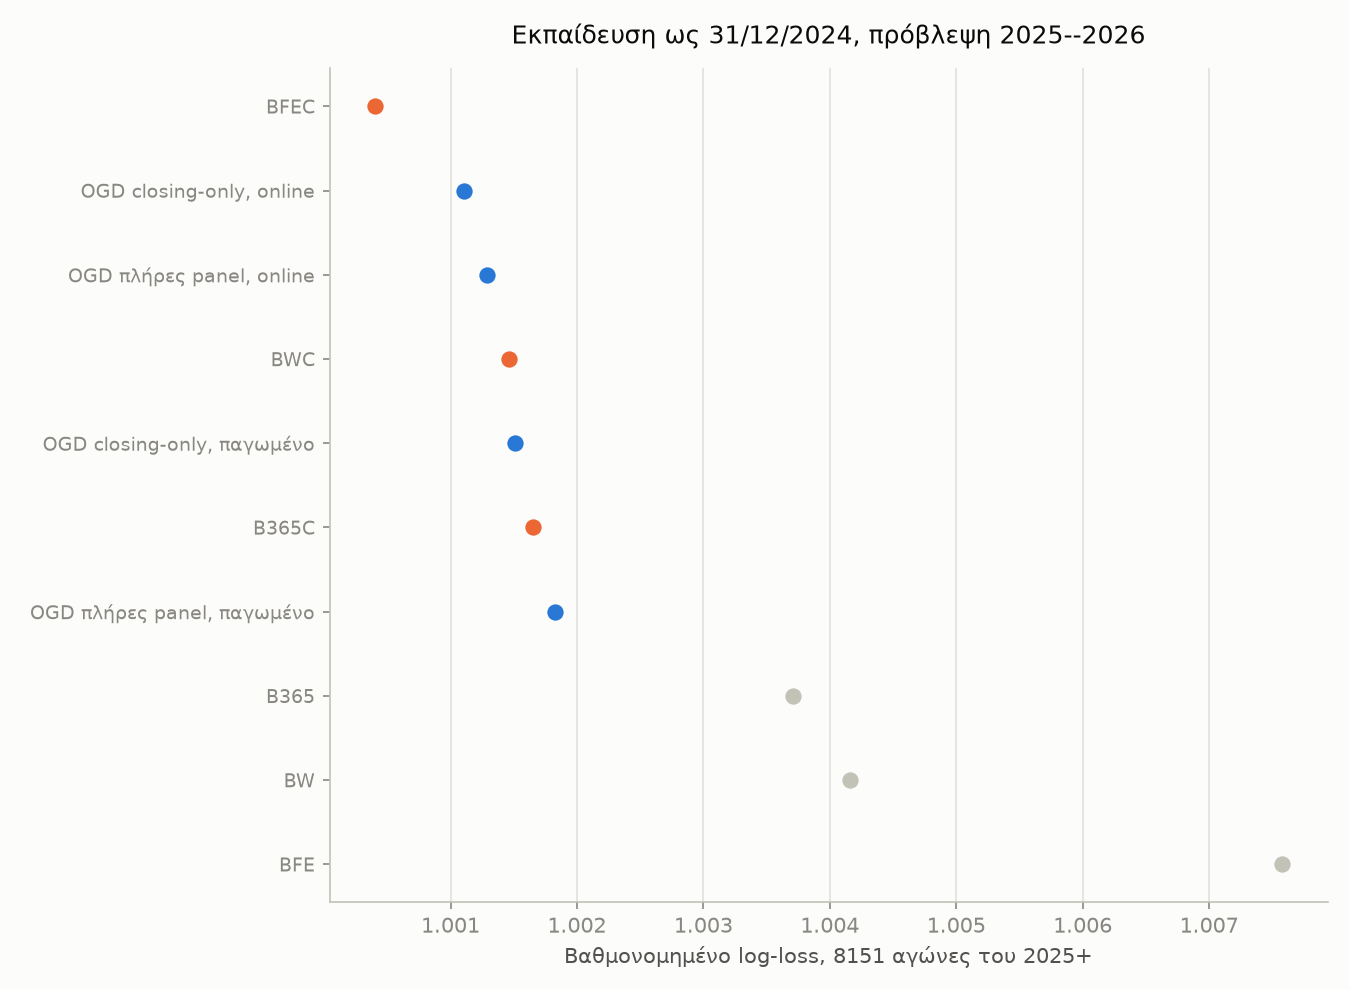
\includegraphics[width=0.92\linewidth]{deployment_test.png}
  \caption{Έλεγχος ανάπτυξης. Οι τιμές ανοίγματος βρίσκονται σαφώς χαμηλότερα, ενώ οι τιμές κλεισίματος και οι παραλλαγές του μείγματος συγκεντρώνονται.}
  \label{fig:deploy}
\end{figure}

\begin{itemize}
  \item \textbf{Κάθε τιμή ανοίγματος κερδίζεται σημαντικά}, σε κάθε παραλλαγή: $-0{,}0019$
        έως $-0{,}0065$, όλα $p\leq0{,}019$.
  \item \textbf{Οι τιμές κλεισίματος δεν κερδίζονται.} Το βέλτιστο αποτέλεσμα είναι ισοπαλία
        και με τις τρεις, και μόνο στην παραλλαγή closing-only / online: B365C $p=0{,}193$,
        BWC $p=0{,}361$, BFEC $p=0{,}052$. Στις παραλλαγές πλήρους panel το \textbf{BFEC μάς
        κερδίζει σημαντικά} ($+0{,}00089$, $p=0{,}013$ online· $+0{,}00143$, $p=0{,}002$
        παγωμένο), οπότε η ισοπαλία με κάθε τιμή κλεισίματος ισχύει μόνο για τη
        closing-only παραλλαγή.
  \item Η online παραλλαγή κερδίζει σταθερά την παγωμένη ($1{,}00110$ έναντι $1{,}00151$),
        οπότε η ακριβής διατύπωση δεν είναι «εκπαιδεύτηκε ως το 2024» αλλά «τρέχει συνεχώς».
\end{itemize}

\paragraph{Η Pinnacle σε αυτό το παράθυρο.} Η κάλυψή της πέφτει στο 59\% μετά το 2025 και
σταματάει να δίνει αποδόσεις στις 14/01/2026, οπότε δεν περνάει το κατώφλι. Επιβάλλοντάς την
στον κοινό πίνακα, οι κοινοί αγώνες πέφτουν από 8.151 σε 2.860 και κανένα αποτέλεσμα δεν
παραμένει σημαντικό. Συγκρίνεται επομένως ένα προς ένα, στους δικούς της γύρους: τον PS τον
κερδίζουμε σημαντικά ($-0{,}0022$ έως $-0{,}0023$, $p$ από $0{,}007$ ως $0{,}019$, σε 6.857
αγώνες) και με τον PSC ισοπαλούμε ($p$ από $0{,}532$ ως $0{,}796$, σε 6.892 αγώνες).

Αξίζει να σημειωθεί ότι ο καλύτερος προγνώστης σε αυτό το παράθυρο δεν είναι bookmaker αλλά
το \textbf{Betfair Exchange}: ανταλλακτήριο όπου οι παίκτες στοιχηματίζουν μεταξύ τους,
δηλαδή τιμή αγοράς χωρίς περιθώριο διαχειριστή.

\section{Value betting και το μαθαινόμενο μέγεθος στοιχήματος}
\label{sec:res-value}

Προσομοίωση Kelly με βαθμονομημένες πιθανότητες και panel ταιριασμένο στη φάση του στόχου.
Το μέγεθος του στοιχήματος δεν καθηλώνεται σε σταθερό κλάσμα αλλά μαθαίνεται online, με τον
πολλαπλασιαστή του \S\ref{sec:oco-kelly-theory}· ο σταθερός συντελεστής $\tfrac14$ κρατιέται
ως σημείο αναφοράς.

\paragraph{Έλεγχος ορθότητας και επιλογή.} Σταθερό $\lambda = 0{,}25$ αναπαράγει
\emph{ακριβώς} την υλοποιημένη προσομοίωση, σε κάθε γύρο ανάπτυξης και στο ίδιο σύνολο
στοιχημάτων, οπότε ο μαθαινόμενος πολλαπλασιαστής είναι η μόνη διαφορά μεταξύ των στηλών που
ακολουθούν. Το ρυθμό, την αρχική τιμή και το άνω όριο του $\lambda$ τα επιλέγουμε σε
χρονολογικό πρόθεμα $75\%$ των \emph{στοιχημάτων}, από κοινού για όλους τους στόχους, και η
υπόλοιπη ουρά μένει έξω από την επιλογή. Τίποτα από τα δύο προηγούμενα στάδια δεν
ξανασυντονίζεται εδώ.

Η επιλογή δίνει $\lambda_0 = 0{,}5$ και $\lambda_{\max} = 1{,}5$ για το Online Newton Step,
με ουρά $+0{,}000106$ σε λογαριθμικό ρυθμό ανά στοίχημα, και $\lambda_0 = 0{,}25$,
$\lambda_{\max} = 1$ για τον OGD, με ουρά $+0{,}000101$. Αξίζει να σημειωθεί ένα σημείο που
έρχεται σε αντίθεση με κάθε άλλο συντονισμό της εργασίας: \textbf{το Online Newton Step
επιλέγει πολλαπλασιαστή ρυθμού ίσο με $1$}, δηλαδή η σταθερά που δίνει η θεωρία δεν
χρειάζεται καμία διόρθωση, ενώ ο OGD χρειάζεται $\times 10$ και σε μία ρύθμιση το πλέγμα
φεύγει στην ακμή χωρίς να σταθεροποιηθεί. Όπου η δομή της απώλειας αξιοποιείται σωστά, το
a-priori φράγμα αποδεικνύεται και σωστά βαθμονομημένο.

\begin{table}[H]
\centering
\small
\begin{tabular}{@{}lrrrrr@{}}
\toprule
\textbf{Εναντίον} & \textbf{Στοιχ.} & \textbf{Kelly $\tfrac14$} & \textbf{OCO $\lambda$} &
\textbf{Kelly πλήρες} & \textbf{μέσο $\lambda$} \\
\midrule
WHC     &  7.253 & $84{,}2\times$  & $\mathbf{6.494\times}$   & $29.342\times$   & 0,79 \\
BWC     &  6.920 & $3{,}09\times$  & $\mathbf{7{,}08\times}$  & $13{,}77\times$  & 0,62 \\
VC\_BVC &  4.561 & $1{,}58\times$  & $1{,}54\times$           & $1{,}74\times$   & 0,57 \\
B365C   &  7.643 & $1{,}05\times$  & $0{,}67\times$           & $0{,}24\times$   & 0,39 \\
PSC     & 19.497 & $0{,}54\times$  & $0{,}25\times$           & $0{,}0035\times$ & 0,37 \\
\bottomrule
\end{tabular}
\caption{Τελικό κεφάλαιο με αρχή $1$, βαθμονομημένες πιθανότητες, απλή κανονικοποίηση.
Κάθε στήλη παίζει τα \emph{ίδια} στοιχήματα, αφού η επιλογή ενδεχομένου δεν εξαρτάται από το
μέγεθος. Η τελευταία στήλη είναι ο μέσος πολλαπλασιαστής που έμαθε το Online Newton Step.}
\label{tab:oco-kelly}
\end{table}

\begin{figure}[H]
\centering
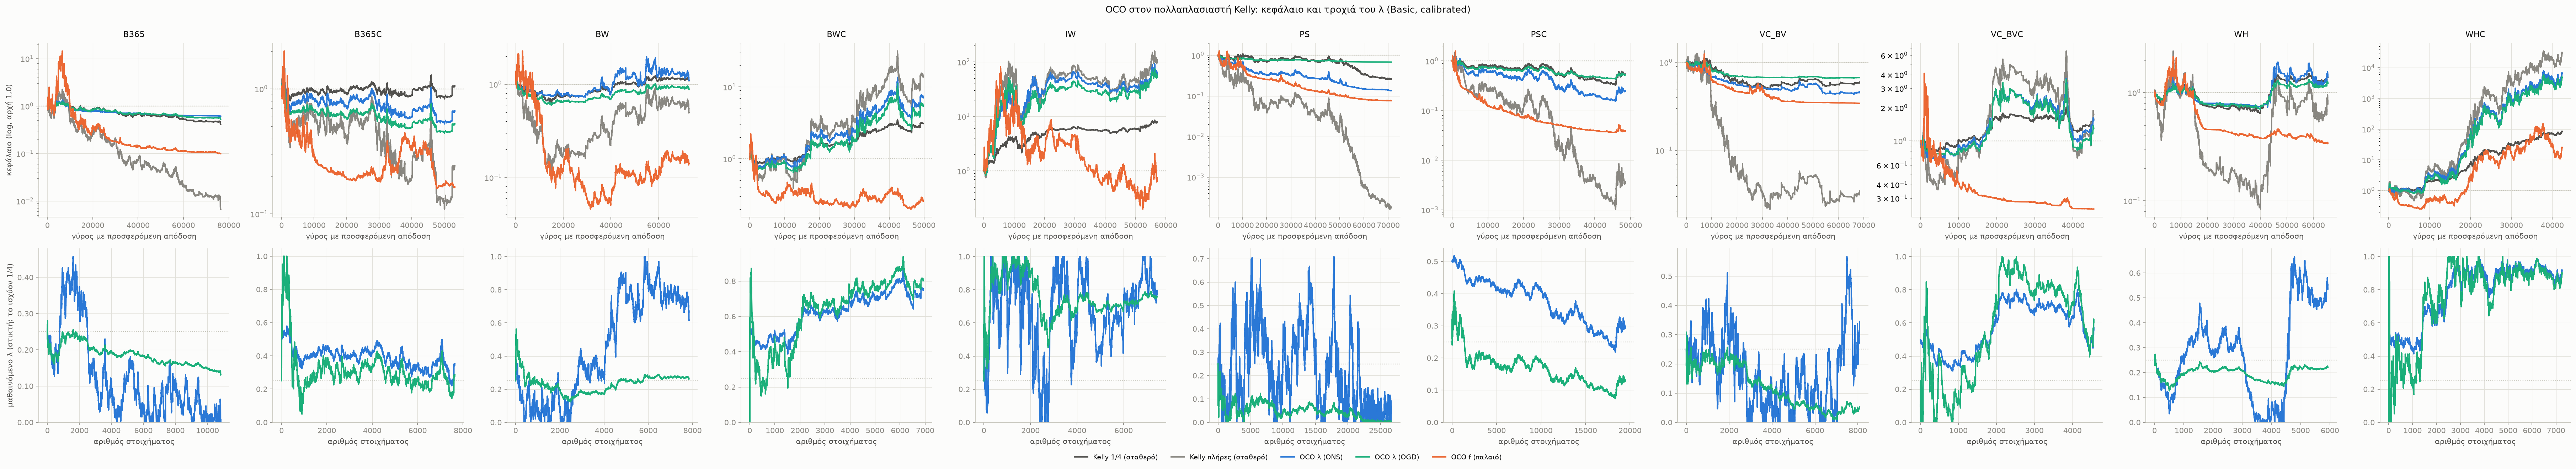
\includegraphics[width=\textwidth]{oco_kelly.png}
\caption{Πάνω, η πορεία του κεφαλαίου· κάτω, η τροχιά του μαθαινόμενου $\lambda$ με στικτή
γραμμή στο ισχύον $\tfrac14$.}
\end{figure}

\paragraph{Το αποτέλεσμα έχει δύο σκέλη που δεν λένε το ίδιο.} Στον ζευγαρωμένο έλεγχο ανά
στοίχημα ο μαθαινόμενος πολλαπλασιαστής \textbf{ισοπαλεί} με το σταθερό $\tfrac14$: σε είκοσι
κελιά (δύο κανονικοποιήσεις $\times$ δύο στάδια $\times$ πέντε στόχοι) προκύπτουν 17
ισοπαλίες, δύο νίκες και μία ήττα. Στο τελικό κεφάλαιο είναι μπροστά σε δύο από τους
πέντε στόχους, και στον WHC κατά εβδομήντα επτά φορές. Τα δύο συμβιβάζονται αριθμητικά: η
διαφορά ανά στοίχημα είναι $+0{,}00060$, μικροσκοπική, αλλά ανατοκίζεται σε $7.253$
στοιχήματα, ενώ η αβεβαιότητα παραμένει αρκετά πλατιά ώστε ο έλεγχος να μην την πιστοποιεί
($p=0{,}099$). Είναι
το ίδιο μοτίβο με το αποτέλεσμα του «σκληρού» άγκυρα-bookmaker: συστηματική υπεροχή στο
σημειακό μέγεθος, χωρίς στατιστική πιστοποίηση.

\paragraph{Τι μαθαίνει ο πολλαπλασιαστής.} Κάθεται σχεδόν παντού πάνω από το $\tfrac14$, και
η τιμή του παρακολουθεί το πόσο κερδοφόρος είναι ο στόχος: $0{,}37$ στον ζημιογόνο PSC,
$0{,}79$ στον κερδοφόρο WHC. Ανεβάζει δηλαδή το ρίσκο
όπου υπάρχει περιθώριο και το μαζεύει όπου δεν υπάρχει --- συμπεριφορά που καμία σταθερά δεν
μπορεί να εκφράσει, και η οποία προκύπτει χωρίς να του δοθεί καμία πληροφορία για το ποιος
είναι ο αντίπαλος.

\paragraph{Η διατύπωση ήταν το πρόβλημα, όχι η ιδέα.} Η ίδια ερώτηση είχε τεθεί νωρίτερα με
τον μαθητή να μαθαίνει απευθείας το \emph{κλάσμα} του κεφαλαίου. Εκείνη η εκδοχή έχανε
συστηματικά: 9 ήττες στα 20 κελιά, καμία νίκη. Η αιτία είναι ακριβώς αυτή που προβλέπει το
\S\ref{sec:oco-kelly-theory} --- ο comparator «καλύτερο σταθερό ποντάρισμα» δεν περιέχει τον
κλειστό τύπο, και ο μαθητής πετά το $\hat{p}_t$ που τα δύο προηγούμενα στάδια μόλις
παρήγαγαν. Αλλάζοντας μόνο το τι μαθαίνεται, με τα ίδια δεδομένα και τον ίδιο έλεγχο, το
αποτέλεσμα περνά από συστηματική ήττα σε ισοπαλία με σημειακή υπεροχή.

\paragraph{Παράπλευρο εύρημα: το $\tfrac14$ είναι υπερβολικά συντηρητικό.} Το \emph{πλήρες}
Kelly ισοπαλεί σε 16 από τα 20 κελιά, κερδίζει σε 2 και χάνει μόνο σε 2. Ο κίνδυνός του
συγκεντρώνεται σχεδόν ολόκληρος στον PSC, όπου μηδενίζει το κεφάλαιο ($0{,}0035$). Στους κερδοφόρους
στόχους δηλαδή το σταθερό $\tfrac14$ αφήνει σημαντικό μέρος της ανάπτυξης αχρησιμοποίητο. Ο
μαθαινόμενος πολλαπλασιαστής είναι ο ενδιάμεσος δρόμος: κρατά το μεγαλύτερο μέρος της ανόδου
και αποφεύγει την καταστροφή.

\paragraph{Πού υπάρχει άκρη.} Το ποιοι bookmakers είναι καν κερδίσιμοι χαρτογραφείται σε δέκα
στόχους με το σταθερό $\tfrac14$, ώστε οι γραμμές να παραμένουν συγκρίσιμες μεταξύ τους.

\begin{table}[H]
\centering
\small
\begin{tabular}{@{}llrrrl@{}}
\toprule
\textbf{Εναντίον} & \textbf{Φάση} & \textbf{Στοιχ.} & \textbf{Κεφάλαιο} & \textbf{$p$} & \\
\midrule
WHC     & closing & 6.565  & $38{,}52\times$ & $<0{,}001$ & κέρδος \\
IW      & opening & 7.443  & $7{,}89\times$  & $0{,}008$  & κέρδος \\
\midrule
BWC     & closing & 6.607  & $1{,}81\times$  & $0{,}247$ & --- \\
WH      & opening & 5.931  & $1{,}38\times$  & $0{,}545$ & --- \\
BW      & opening & 7.841  & $1{,}09\times$  & $0{,}820$ & --- \\
VC\_BVC & closing & 4.653  & $0{,}75\times$  & $0{,}455$ & --- \\
VC\_BV  & opening & 8.083  & $0{,}60\times$  & $0{,}245$ & --- \\
B365C   & closing & 7.970  & $0{,}58\times$  & $0{,}328$ & --- \\
B365    & opening & 10.829 & $0{,}41\times$  & $0{,}101$ & --- \\
PS      & opening & 26.675 & $0{,}26\times$  & $0{,}055$ & --- \\
\midrule
PSC     & closing & 39.997 & $0{,}0002\times$ & $<0{,}001$ & ζημιά \\
\bottomrule
\end{tabular}
\caption{Η στήλη $p$ αφορά τον μέσο λογαριθμικό ρυθμό ανά στοίχημα. Τα τελικά κεφάλαια δεν
συγκρίνονται μεταξύ γραμμών, αφού ο αριθμός στοιχημάτων διαφέρει κατά τάξη μεγέθους.}
\end{table}

Σε έντεκα bookmakers προκύπτουν \emph{δύο} σημαντικά κέρδη --- και οι δύο απέναντι σε
«μαλακούς», recreational-facing οίκους --- και μία σημαντική ζημιά, απέναντι στον PSC, που
είναι ο καλύτερος προγνώστης του panel και επομένως ακριβώς ο αντίπαλος απέναντι στον οποίο
ένα κατώτερο μοντέλο οφείλει να χάνει. Ο έλεγχος λειτουργεί δηλαδή και προς τις δύο
κατευθύνσεις. Η αντιστοίχιση φάσης είναι ουσιώδης: με το πλήρες panel αντί για το
closing-only, το αποτέλεσμα χειροτερεύει σε \emph{κάθε} έναν από τους closing στόχους.

\paragraph{Η επέκταση στους στόχους ανοίγματος.} Ο μαθαινόμενος πολλαπλασιαστής εφαρμόζεται
και στους έξι opening στόχους, με το αντίστοιχο opening-only panel. Η απαίτηση αιτιότητας
είναι εδώ αυστηρότερη: δεν αρκεί να φύγει ο στόχος, πρέπει να φύγει \emph{ολόκληρη} η closing
πλευρά, αφού καμία τιμή κλεισίματος δεν υπάρχει τη στιγμή που τοποθετείται το στοίχημα. Οι
υπερπαράμετροι επιλέγονται χωριστά ανά φάση, στο δικό της πρόθεμα στοιχημάτων, ώστε το
αποτέλεσμα των opening να μην εξαρτάται από στοιχήματα των closing.

\begin{table}[H]
\centering
\small
\begin{tabular}{@{}lrrrrr@{}}
\toprule
\textbf{Εναντίον} & \textbf{Στοιχ.} & \textbf{Kelly $\tfrac14$} & \textbf{OCO $\lambda$} &
\textbf{Kelly πλήρες} & \textbf{μέσο $\lambda$} \\
\midrule
IW      &  7.443 & $7{,}89\times$  & $\mathbf{64{,}4\times}$ & $109{,}6\times$  & 0,67 \\
WH      &  5.931 & $1{,}38\times$  & $1{,}39\times$          & $0{,}78\times$   & 0,28 \\
BW      &  7.841 & $1{,}09\times$  & $1{,}10\times$          & $0{,}50\times$   & 0,45 \\
VC\_BV  &  8.083 & $0{,}60\times$  & $0{,}67\times$          & $0{,}03\times$   & 0,17 \\
B365    & 10.829 & $0{,}41\times$  & $0{,}61\times$          & $0{,}007\times$  & 0,12 \\
PS      & 26.675 & $0{,}26\times$  & $\mathbf{0{,}68\times}$ & $0{,}0003\times$ & 0,05 \\
\bottomrule
\end{tabular}
\caption{Στόχοι ανοίγματος: τελικό κεφάλαιο με αρχή $1$, βαθμονομημένες πιθανότητες, απλή
κανονικοποίηση. Η στήλη OCO $\lambda$ δίνει την καλύτερη από τις δύο παραλλαγές (ONS / OGD)
και το μέσο $\lambda$ αντιστοιχεί σε αυτήν.}
\label{tab:oco-kelly-opening}
\end{table}

Το εύρημα είναι ότι ο μαθαινόμενος πολλαπλασιαστής αποδίδει \emph{περισσότερο} στα ανοίγματα
παρά στα κλεισίματα: 8 νίκες και 2 ήττες σε 48 ζευγαρωμένους ελέγχους, έναντι 4 νικών και 3
ηττών στα κλεισίματα. Σημαντικές νίκες προκύπτουν απέναντι στους PS ($p<0{,}001$), IW
($p=0{,}027$) και VC\_BV ($p=0{,}009$), ενώ οι δύο ήττες είναι μικροσκοπικές
($-0{,}000028$ και $-0{,}000080$).

Πιο ενδιαφέρον από το αποτέλεσμα είναι ο \emph{μηχανισμός}, που εδώ γίνεται ορατός. Το μέσο
$\lambda$ κατατάσσει τους στόχους σχεδόν τέλεια κατά το πόσο είναι νικήσιμοι, χωρίς να δοθεί
στον αλγόριθμο καμία πληροφορία για το ποιος είναι ο αντίπαλος: στον IW, τον μόνο κερδοφόρο
στόχο ανοίγματος, ανεβάζει το $\lambda$ στο $0{,}67$, δηλαδή σχεδόν στο πλήρες Kelly· στον PS,
τον σκληρότερο, το κατεβάζει στο $0{,}05$ και ουσιαστικά σταματά να στοιχηματίζει ---
υπερδιπλασιάζοντας έτσι το κεφάλαιο που επιβιώνει, από $0{,}26\times$ σε $0{,}68\times$. Τα
$\lambda$ των ανοιγμάτων ($0{,}05$--$0{,}75$) είναι συστηματικά χαμηλότερα από εκείνα των
κλεισιμάτων ($0{,}17$--$0{,}79$): η αγορά ανοίγματος είναι δυσκολότερη και ο αλγόριθμος το
ανακαλύπτει μόνος του.

Το ίδιο φαίνεται και από την αντίθετη πλευρά. Το \emph{πλήρες} Kelly, που στα κλεισίματα
ισοπαλούσε (2 νίκες, 2 ήττες), στα ανοίγματα καταρρέει: \textbf{11 σημαντικές ήττες έναντι 2
νικών}. Η πλευρά του ανοίγματος χρειάζεται δηλαδή πραγματικά συρρίκνωση, και το ερώτημα δεν
είναι αν θα επιβληθεί αλλά πόση --- που είναι ακριβώς το ερώτημα στο οποίο ένας σταθερός
συντελεστής $\tfrac14$ δεν μπορεί να απαντήσει και ένας μαθαινόμενος μπορεί.

Το συμπέρασμα είναι ότι το βελτιωμένο log-loss δεν μεταφράζεται σε κερδοφορία. Η διαφορά
ποιότητας που κερδήθηκε είναι μικρότερη από το περιθώριο της αγοράς, και όποια άκρη υπάρχει
αφορά \emph{συγκεκριμένους} bookmakers, όχι στρατηγική που δουλεύει γενικά. Το μέγεθος του
στοιχήματος είναι ορθογώνιο σε αυτό: αλλάζει πόσο γρήγορα μεγαλώνει το κεφάλαιο εκεί που
άκρη υπάρχει, και πόσο γρήγορα χάνεται εκεί που δεν υπάρχει, χωρίς να δημιουργεί άκρη από το
μηδέν.

\section{Πόση πληροφορία χρειάζεται η μάθηση; Το bandit πείραμα}
\label{sec:res-bandit}

Όλα τα προηγούμενα προϋποθέτουν πλήρη πληροφόρηση: μετά από κάθε αγώνα βαθμολογούνται και οι
$26$ bookmakers. Το ερώτημα του \S\ref{sec:bandit-theory} είναι τι απομένει όταν ο
αλγόριθμος βλέπει μόνο \emph{έναν} αριθμό τον γύρο, την απώλεια της δικής του πρόβλεψης.
Υλοποιούνται οι δύο εκτιμητές κλίσης, ενός και δύο σημείων, με τα $\xi$ και το βήμα
επιλεγμένα στο ίδιο χρονολογικό train prefix με κάθε άλλη υπερπαράμετρο, και δέκα
διαφορετικούς σπόρους τυχαιότητας, αφού ο αλγόριθμος είναι στοχαστικός.

Δύο έλεγχοι ορθότητας προηγούνται. Με πλήρη πληροφόρηση και γραμμικοποιημένη απώλεια ο
κώδικας αναπαράγει \emph{ακριβώς} τον υλοποιημένο OGD, και ο εκτιμητής δύο σημείων
ταυτοποιείται με την αληθινή εφαπτομενική κλίση με σχετικό σφάλμα $0{,}6\%$ και συνημίτονο
$0{,}99998$ πάνω σε $200.000$ δείγματα.

\begin{table}[H]
\centering
\small
\begin{tabular}{lrrr}
\toprule
Σειρά & Βαθμ.\ log-loss & Raw log-loss & Διαφορά \\
\midrule
OGD, πλήρης πληρ., ακριβής κλίση & 0,996928 & 0,997455 & $+0{,}000002$ \\
OGD, πλήρης πληρ., γραμμικοποίηση & 0,996926 & 0,997454 & --- \\
BGD δύο σημείων ($\xi=0{,}0003$) & 0,997368 & 0,998004 & $+0{,}000443$ \\
\emph{Χωρίς μάθηση} ($\eta=0$) & 0,997632 & 0,998296 & $+0{,}000707$ \\
BGD ενός σημείου ($\xi=0{,}02$) & 0,997631 & 0,998297 & $+0{,}000706$ \\
Ομοιόμορφος μέσος & 0,998132 & 0,998862 & $+0{,}001206$ \\
\bottomrule
\end{tabular}
\caption{Bandit έναντι πλήρους πληροφόρησης, ίδιοι 76.584 γύροι, ίδιο calibration. Η
τελευταία στήλη είναι η ζευγαρωμένη διαφορά από τον υλοποιημένο OGD στο βαθμονομημένο
log-loss· θετική σημαίνει χειρότερο από αυτόν. Η πρώτη γραμμή είναι ισοπαλία
($p=0{,}823$), οι υπόλοιπες σημαντικές σε $p<0{,}001$.}
\label{tab:bandit}
\end{table}

\begin{figure}[H]
\centering
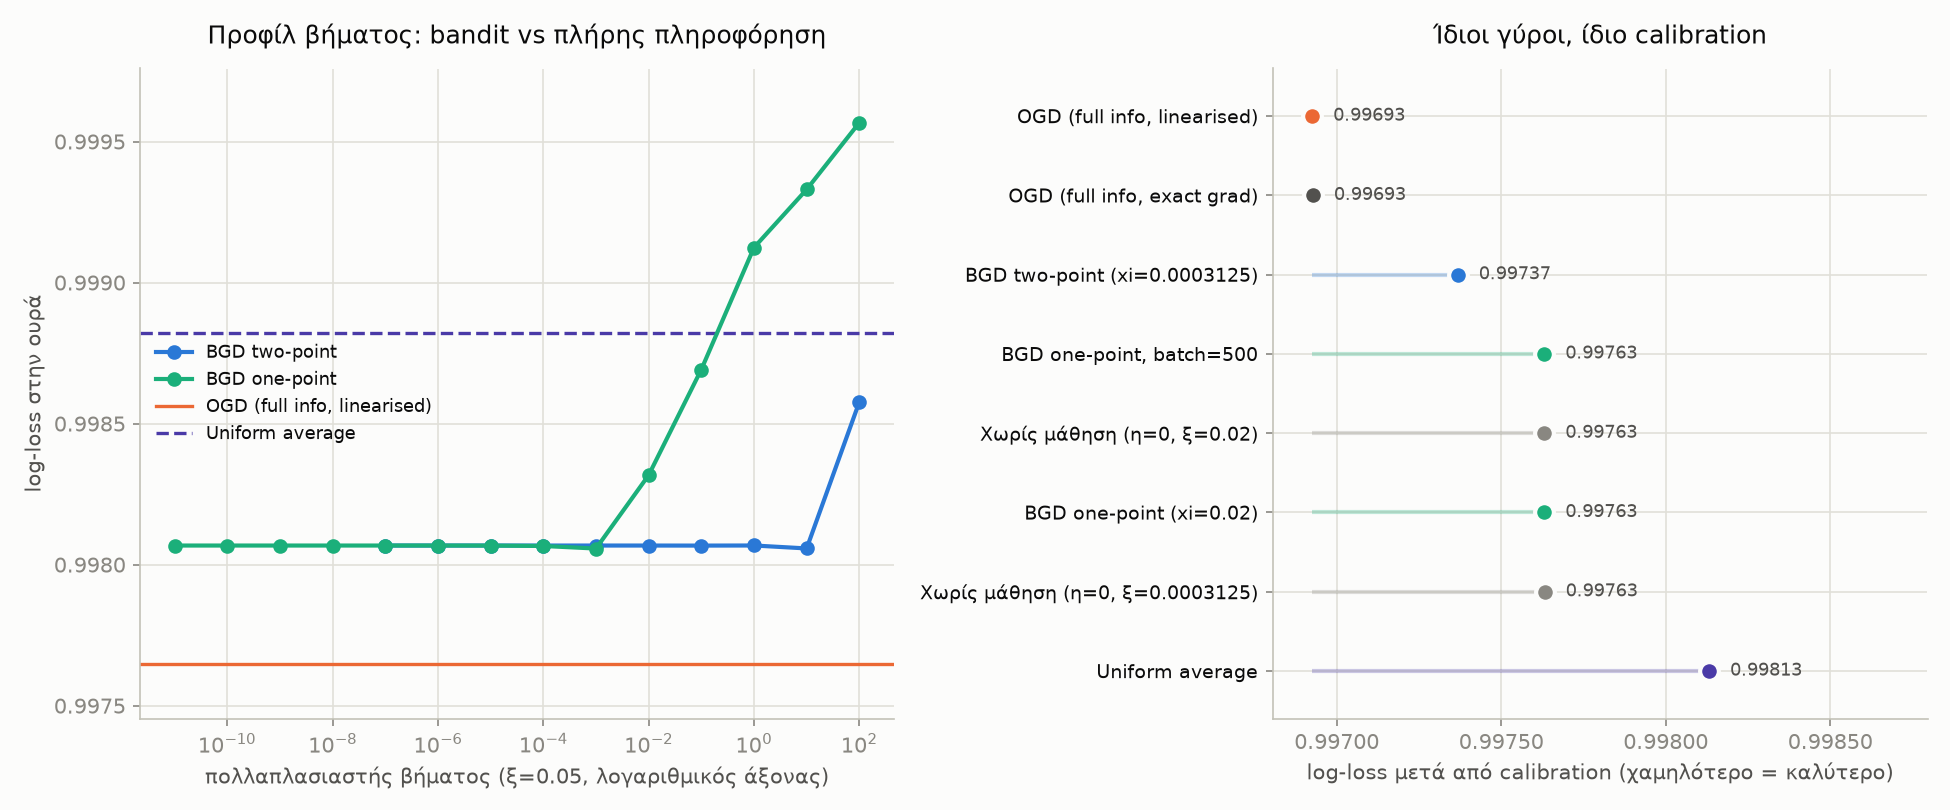
\includegraphics[width=\textwidth]{bandit_oco.png}
\caption{Αριστερά, το προφίλ του βήματος πάνω στο οποίο γίνεται η επιλογή· δεξιά, η τελική
σύγκριση.}
\end{figure}

\paragraph{Ο έλεγχος που κάνει τους αριθμούς ερμηνεύσιμους.} Η προφανής ανάγνωση --- «το BGD
ξεπερνά τον ομοιόμορφο μέσο, άρα η bandit ανάδραση του δίδαξε κάτι» --- είναι λανθασμένη, και
η εργασία την έκανε σε πρώτη γραφή πριν τη διορθώσει. Υπό την αναγωγή Sleeping Experts το
διάνυσμα βαρών κινείται ακόμη και με \emph{μηδενικό} βήμα: κάθε φορά που αλλάζει το σύνολο
των ξύπνιων, η μόνιμη κατάσταση επαναπροβάλλεται σε simplex άλλης διάστασης, και αυτή η
αναταραχή από μόνη της παράγει μη ομοιόμορφα βάρη. Μετρημένο απευθείας: στο $\eta=0$ τα βάρη
απέχουν ως $0{,}69$ από το ομοιόμορφο σε νόρμα μεγίστου. Ο σωστός συγκριτικός δείκτης δεν
είναι επομένως ο ομοιόμορφος μέσος αλλά ο \emph{ίδιος ο αλγόριθμος με το βήμα στο μηδέν}:
ίδια συρρίκνωση, ίδιες διαταραχές, ίδια δυναμική προβολής, καμία μάθηση. Ό,τι βρίσκεται
ανάμεσα στον έλεγχο αυτόν και στο BGD είναι ό,τι αγόρασε πράγματι το bandit σήμα.

\begin{table}[H]
\centering
\small
\begin{tabular}{lrr}
\toprule
& \textbf{Προβολή χωρίς μάθηση} & \textbf{$+$ bandit μάθηση} \\
\midrule
BGD δύο σημείων & $+0{,}000500$ \;(41,4\%) & $+0{,}000264$ \;(21,9\%) \\
BGD ενός σημείου & $+0{,}000501$ \;(41,5\%) & $\mathbf{-0{,}000000}$ \;(0,0\%) \\
\bottomrule
\end{tabular}
\caption{Διάσπαση του περιθωρίου πλήρους πληροφόρησης (ομοιόμορφος μέσος $0{,}998132$ προς
OGD $0{,}996926$, δηλαδή $0{,}001206$) σε ό,τι δίνει η προβολή χωρίς καμία μάθηση και σε ό,τι
προσθέτει από πάνω η bandit ανάδραση.}
\label{tab:bandit-decomp}
\end{table}

\paragraph{Ο εκτιμητής ενός σημείου δεν μαθαίνει τίποτα εδώ.} Η επιλογή στο train οδηγεί το
βήμα του στο $1{,}4\cdot10^{-14}$, και ολόκληρη η περιοχή από $10^{-14}$ ως $9\cdot10^{-11}$
ισοβαθμεί στο ίδιο train score $0{,}998375$: πρόκειται για το οροπέδιο της μη μάθησης, και ο
επιλογέας απλώς παίρνει το άκρο του. Κάθε θετική ποσότητα μάθησης βλάπτει. Η αιτία
ποσοτικοποιείται από την ευθυγράμμιση της εκτίμησης ενός γύρου με την αληθινή κλίση: για τον
εκτιμητή δύο σημείων το μέσο συνημίτονο είναι $+0{,}27$, ενώ για τον εκτιμητή ενός σημείου
$+0{,}002$, δηλαδή μηδέν. Το σήμα είναι $0{,}2\%$ του μεγέθους της εκτίμησης· η άθροιση σε
$T$ γύρους μειώνει τον θόρυβο κατά $\sqrt{T}\approx277$, που αφήνει ωφέλιμο λόγο περίπου
$0{,}55$ --- ακόμη κάτω από τη μονάδα. \textbf{Ο ορίζοντας δεν επαρκεί} για εκτιμητή ενός
σημείου πάνω σε simplex $25$ διαστάσεων.

\paragraph{Η μία θεμιτή διόρθωση δοκιμάστηκε και δεν αλλάζει τίποτα.} Το επιχείρημα της
διασποράς υπαγορεύει μια συγκεκριμένη παρέμβαση: συσσώρευση της εκτίμησης για $m$ γύρους πριν
το βήμα, που ανεβάζει τον ωφέλιμο λόγο κατά $\sqrt{m}$ και κρατά το σημείο στο εσωτερικό του
simplex, ώστε η προβολή να μην αποκόπτει ασύμμετρα τον θόρυβο. Σαρώθηκε $m$ σε
$\{1,20,100,500\}$ επί πέντε τάξεις μεγέθους του βήματος. \emph{Κανένας} συνδυασμός δεν
παράγει εσωτερικό βέλτιστο: κάθε κελί είναι είτε πάνω στο οροπέδιο είτε χειρότερο, και το
batching κάνει ακριβώς ό,τι προβλέπει η θεωρία --- ανέχεται μεγαλύτερο βήμα χωρίς ζημιά ---
χωρίς ποτέ να παράγει κέρδος. Το σήμα δεν υπάρχει για να ενισχυθεί.

\paragraph{Μια επιφύλαξη για τον εκτιμητή δύο σημείων.} Η παράμετρος συρρίκνωσής του
οδηγήθηκε από την επιλογή στο κάτω όριο του επιτρεπτού διαστήματος. Αυτό δεν είναι ατύχημα
αλλά το αναμενόμενο: καθώς $\delta\to 0$ η πεπερασμένη διαφορά συγκλίνει στην ακριβή
κατευθυντική παράγωγο, οπότε ο εκτιμητής δύο σημείων \emph{παύει να είναι bandit}. Το
$21{,}9\%$ του Πίνακα~\ref{tab:bandit-decomp} πρέπει επομένως να διαβάζεται ως άνω φράγμα
του τι πετυχαίνει η προσέγγιση με δύο ερωτήματα, όχι ως επίδοση σε γνήσιο bandit
περιβάλλον. Ο εκτιμητής ενός σημείου είναι το ειλικρινές πείραμα, και η απάντησή του είναι
μηδέν.

\paragraph{Τι μένει από το πείραμα.} Δύο πράγματα, και κανένα τους δεν είναι αυτό που
αναζητούσε. Πρώτον, ότι η ανάδραση ενός σημείου είναι ανεπαρκής σε αυτόν τον ορίζοντα, με
ποσοτική εξήγηση του γιατί και με την προφανή διόρθωση δοκιμασμένη και απορριφθείσα.
Δεύτερον, και πιο χρήσιμο για την υπόλοιπη εργασία, ότι \textbf{το $41\%$ του περιθωρίου του
μείγματος έναντι του ομοιόμορφου μέσου δεν προέρχεται από μάθηση καθόλου}, αλλά από την
επαναπροβολή που επιβάλλει η μεταβαλλόμενη σύνθεση του panel. Αυτό είναι ανεξάρτητο εύρημα
για τη δυναμική των Sleeping Experts και συμφωνεί με τη μέτρηση του
\S\ref{sec:res-deploy}, όπου η κίνηση των βαρών στα τελευταία στάδια αποδείχθηκε ότι
κυριαρχείται από την προβολή και όχι από το βήμα της κλίσης.

\paragraph{Ένα παράπλευρο εύρημα υπέρ της γραμμικοποίησης.} Ο έλεγχος πλήρους πληροφόρησης
με την \emph{ακριβή} κλίση της μη γραμμικής απώλειας ισοπαλεί με τον υλοποιημένο,
γραμμικοποιημένο OGD ($+0{,}000002$, $p=0{,}934$). Η απλοποίηση του
Λήμματος~\ref{lem:linearization}, δηλαδή, δεν κοστίζει τίποτα μετρήσιμο στα δεδομένα αυτά ---
επιβεβαίωση σχεδιαστικής επιλογής που ως τώρα στηριζόταν μόνο στο θεωρητικό επιχείρημα ότι
το γραμμικό πρόβλημα είναι δυσκολότερο.

\section{Μαρκοβιανή εναλλαγή καθεστώτων αγοράς}
\label{sec:res-regime}

Η μαρκοβιανή αλυσίδα πάνω στο \emph{διάνυσμα βαρών} έχει ήδη δοκιμαστεί και απορριφθεί: κάθε
πυρήνας μετάβασης επιλέγει $\alpha=0$ στο train, δηλαδή καταρρέει στον απλό OGD. Εδώ η
αλυσίδα τρέχει πάνω σε άλλο αντικείμενο --- σε \emph{καταστάσεις της αγοράς}. Διατηρούνται
$K$ λανθάνοντα καθεστώτα, ένα διάνυσμα βαρών ανά καθεστώς υπό Sleeping Experts, και μια
πεποίθηση που ενημερώνεται με την μπροστινή αναδρομή κρυφού μαρκοβιανού μοντέλου· κάθε
καθεστώς βηματίζει ανάλογα με την ευθύνη του. Το $K=1$ αναπαράγει ακριβώς τον
\file{run\_ogd\_sleeping}.

Το κίνητρο είναι μετρημένο και όχι υποθετικό: το \S\ref{sec:res-panels} και η ανάλυση άφιξης
πληροφορίας δείχνουν ότι το πλεονέκτημα των τιμών κλεισίματος ποικίλλει κατά 26 φορές
ανάλογα με το πόσο κινήθηκε η γραμμή. Υπάρχει επομένως πραγματική λανθάνουσα κατάσταση στα
δεδομένα. Το καθεστώς αφήνεται σκόπιμα \emph{λανθάνον}, ώστε να μπορεί να ελεγχθεί εκ των
υστέρων αν η αλυσίδα την ανακαλύπτει μόνη της.

\paragraph{Η πρώτη εκδοχή απέτυχε με διαγνώσιμο τρόπο.} Η μέση πεποίθηση έμεινε στο
$0{,}500$ ακριβώς και για τα δύο καθεστώτα. Τα καθεστώτα \emph{δεν διαφοροποιήθηκαν ποτέ}:
λαμβάνουν το ίδιο διάνυσμα απωλειών, οπότε από συμμετρική αφετηρία ακολουθούν πανομοιότυπες
τροχιές και οι πιθανοφάνειές τους μένουν ίσες. Το αποτέλεσμα ήταν απλώς OGD με βήμα
διαιρεμένο διά $K$, και έχανε σημαντικά ($+0{,}000128$, $p<0{,}001$). Η συμμετρική λύση είναι
σταθερό σημείο της δυναμικής, και χρειάζεται ρητός μηχανισμός διαφοροποίησης.

\paragraph{Μετά τη διόρθωση: ισοπαλία.} Προστέθηκαν οξύτητα πεποίθησης $\beta$, λήθη
$\gamma$, και ρολόι ανά καθεστώς. Η επιλογή στο train δίνει $K=3$, $\beta=30$, $\gamma=0$,
$\tau=0$, με βαθμονομημένο log-loss $0{,}996909$ έναντι $0{,}996926$ του OGD: διαφορά
$-0{,}000016$, $p=0{,}211$, \textbf{ισοπαλία}. Το $\beta=30$ είναι γνήσιο εσωτερικό βέλτιστο
--- το πλέγμα επεκτάθηκε ως το $1000$ και οι τιμές $100$, $300$, $1000$ είναι όλες χειρότερες
στο train.

\paragraph{Δύο ευρήματα που ακυρώνουν κάθε ισχυρισμό ότι «λειτουργεί η αλυσίδα».} Πρώτον, η
ουρά είναι \emph{επίπεδη}: από $\beta=3$ ως $\beta=1000$ κινείται μεταξύ $0{,}997647$ και
$0{,}997649$, εύρος δύο εκατομμυριοστά σε τρεις τάξεις μεγέθους της παραμέτρου, ενώ οι
διαφορές στο train που οδηγούν την επιλογή είναι δεκαπλάσιες. Η επιλογή προσαρμόζεται σε
θόρυβο, όπως ακριβώς στην από κοινού σάρωση βήματος και ρυθμού βαθμονόμησης
(\S\ref{sec:res-negative}). Δεύτερον, και πιο αποφασιστικό, επιλέγεται $\tau=0$ --- καμία
μετάβαση --- και η τυπική απόκλιση της πεποίθησης είναι $0{,}0000$: παγώνει νωρίς και δεν
ξανακινείται. Δεν υπάρχει επομένως μαρκοβιανή εναλλαγή. Ό,τι απομένει είναι σταθερός κυρτός
συνδυασμός τριών OGD με διαφορετική αρχικοποίηση, δηλαδή \emph{ensembling}, και το μικρό
σημειακό κέρδος πρέπει να αποδοθεί σε αυτό.

\paragraph{Και η αλυσίδα δεν ανακαλύπτει τίποτα.} Η συσχέτιση της πεποίθησης με τη μετρημένη
κίνηση της γραμμής είναι μη ορίσιμη, ακριβώς επειδή η πεποίθηση είναι σταθερή. Το λανθάνον
καθεστώς δεν αντιστοιχεί σε καμία μετρήσιμη ιδιότητα της αγοράς. Η απάντηση στο ερώτημα που
έθεσε το πείραμα --- ανακαλύπτει ένα μοντέλο χωρίς πλευρική πληροφορία τη δομή που μετρήθηκε
άμεσα; --- είναι αρνητική και καθαρή.

\begin{figure}[H]
\centering
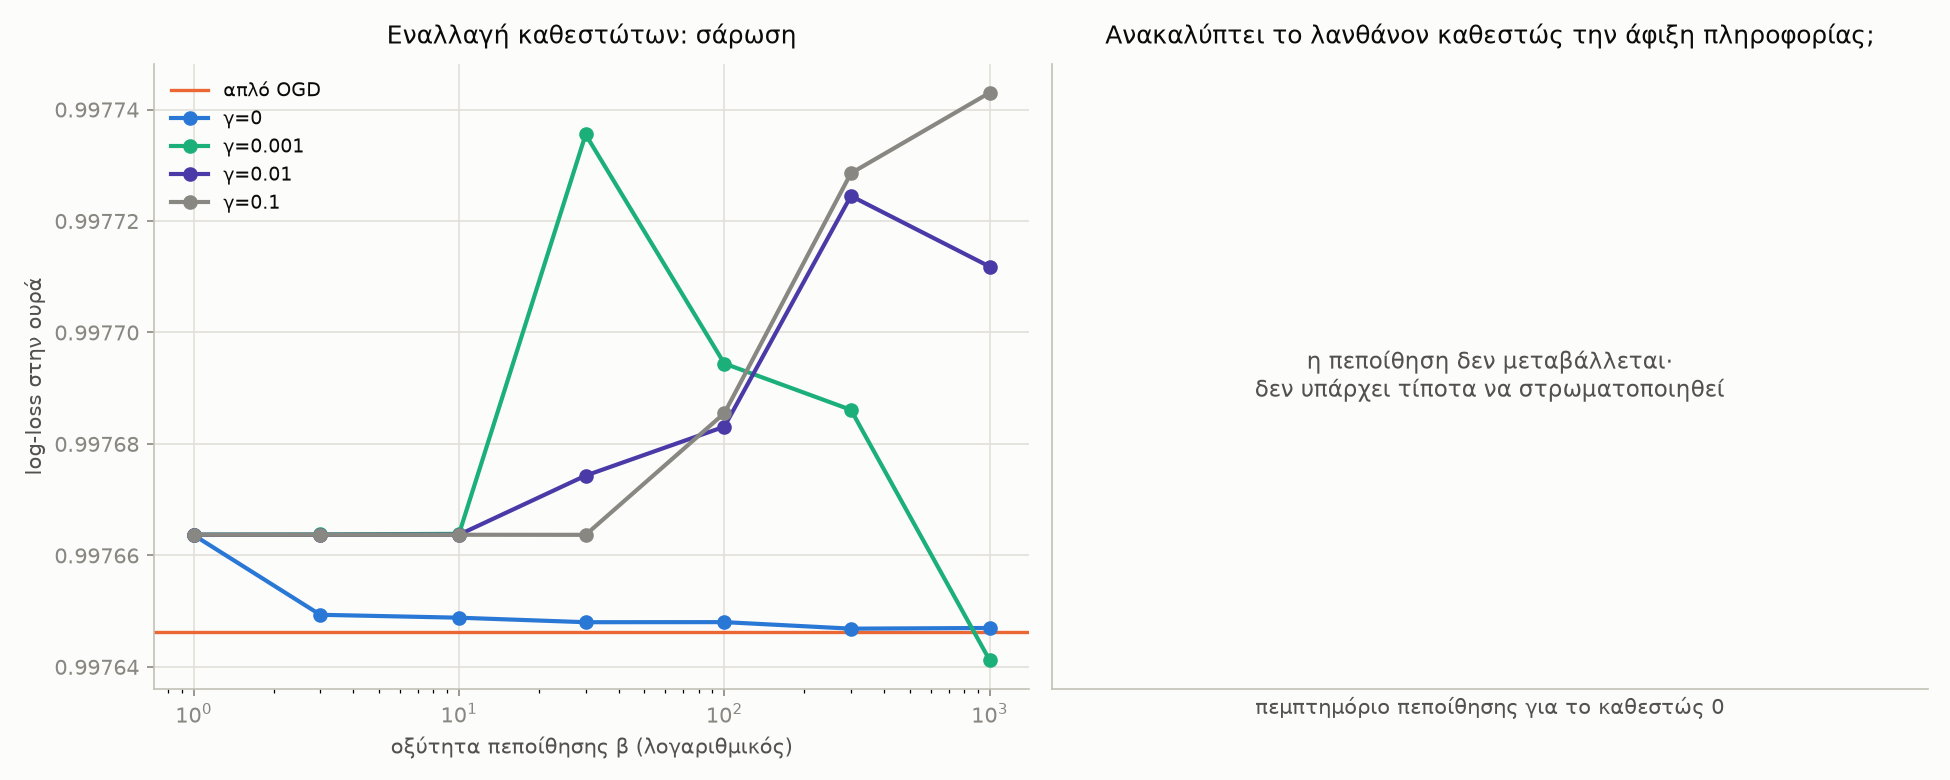
\includegraphics[width=\textwidth]{regime_switching.png}
\caption{Αριστερά, η σάρωση της οξύτητας πεποίθησης. Δεξιά, ο έλεγχος αν το λανθάνον
καθεστώς αντιστοιχεί στη μετρημένη άφιξη πληροφορίας.}
\end{figure}

Πρόκειται για το τρίτο ανεξάρτητο παράδειγμα του ισχυρότερου μοτίβου της εργασίας: μόλις
συντονιστεί το βήμα, καμία μετακίνηση μάζας πάνω στους experts δεν προσφέρει τίποτα
μετρήσιμο. Fixed-Share, πυρήνες μετάβασης, τώρα και εναλλαγή καθεστώτων. Η διαφορά εδώ είναι
ότι η αποτυχία \emph{διαγνώστηκε} αντί απλώς να παρατηρηθεί.

\section{Αρνητικά αποτελέσματα}
\label{sec:res-negative}

Μια σειρά εύλογων υποθέσεων ελέγχθηκε και απορρίφθηκε. Τις αναφέρουμε ρητά, καθώς η καθεμία
περιορίζει το πεδίο εφαρμογής της μεθόδου.

\paragraph{Η εξειδίκευση ανά πρωτάθλημα δεν βοηθάει.} Ένα ξεχωριστό μοντέλο ανά λίγκα χάνει
από το ενιαίο σε \emph{κάθε} μία από τις έξι λίγκες που δοκιμάστηκαν. Δύο εύλογες αιτίες:
κάθε λίγκα διαθέτει μόνο 2.231--3.800 αγώνες, πολύ λίγους για να συγκλίνει ο online
αλγόριθμος αυτόνομα, και οι ειδικοί καταλήγουν να εμπιστεύονται σε μεγάλο βαθμό τους
\emph{ίδιους} experts με το ενιαίο μοντέλο, δηλαδή δεν ανακαλύπτουν κάτι τοπικό.

\paragraph{Το Fixed-Share δεν βοηθάει.} Κάθε $\alpha > 0$ χειροτερεύει το log-loss
($0{,}99842$ στο $\alpha=0$ έναντι $0{,}99885$ και πάνω). Σάρωση του $\alpha$ \emph{από
κοινού} με το βήμα δείχνει γιατί: το $\alpha$ βοηθούσε μόνο όταν το βήμα ήταν πολύ μεγάλο.
Και τα δύο ελέγχουν την ίδια ποσότητα --- πόσο γρήγορα ξεχνάει ο αλγόριθμος --- και το βήμα
είναι το αποδοτικότερο από τα δύο εργαλεία.

\paragraph{Το βήμα ανά expert χειροτερεύει σημαντικά.} Αντικαθιστώντας το καθολικό $t$ με τον
αριθμό των γύρων όπου κάθε expert ήταν ξύπνιος --- που είναι κυριολεκτικά το μέγεθος για το
οποίο μιλά η εγγύηση των Sleeping Experts --- το αποτέλεσμα είναι \emph{καλύτερο στο train
αλλά $-0{,}00073$ στην ουρά}. Ένας expert με κάλυψη 6,9\% λαμβάνει βήμα περίπου 14 φορές
μεγαλύτερο, και το μείγμα κυνηγά τους σπάνιους bookmakers, των οποίων η φαινομενική ποιότητα
είναι συγχυσμένη με τη δυσκολία της μίας σεζόν όπου εμφανίζονται. Πρόκειται για την
καθαρότερη επίδειξη υπερπροσαρμογής στην εργασία.

\paragraph{Η από κοινού επιλογή βήματος και ρυθμού βαθμονόμησης δεν προσφέρει τίποτα.} Οι
δύο παράμετροι δεν αλληλεπιδρούν: ο βέλτιστος ρυθμός βαθμονόμησης είναι $0{,}15$ σε 11 από
11 γραμμές. Η από κοινού επιλογή στο train διαλέγει μάλιστα χειρότερη τιμή για το OGD, καθώς
το πλέγμα είναι εκεί σχεδόν επίπεδο και η επιλογή προσαρμόζεται στον θόρυβο.

\paragraph{Οι μαρκοβιανοί πυρήνες μετάβασης δεν προσφέρουν τίποτα.} Και οι τρεις πυρήνες του
\S\ref{sec:markov-theory}(α) --- ομοιόμορφος, προς τον opening/closing δίδυμο, προς την ίδια
φάση αγοράς --- επιλέγουν $\alpha = 0$ στο χρονολογικό πρόθεμα, δηλαδή καταρρέουν στον απλό
OGD. Οι ζευγαρωμένοι έλεγχοι το επιβεβαιώνουν με μέση διαφορά $0{,}000000$ \emph{ακριβώς} και
$p=1{,}000$, όχι κατά προσέγγιση. Το εύρημα συμφωνεί με το Fixed-Share: από τη στιγμή που το
ίδιο το βήμα είναι συντονισμένο, καμία εκ των υστέρων μετακίνηση μάζας δεν έχει τι να
διορθώσει, γιατί και τα δύο ελέγχουν την ίδια ποσότητα. Αξίζει πάντως να σημειωθεί ότι σε
\emph{μεγάλα} $\alpha$ οι δομημένοι πυρήνες βλάπτουν μετρήσιμα λιγότερο από τον ομοιόμορφο,
δηλαδή η δομή του panel είναι πραγματική και ανιχνεύσιμη --- απλώς περιττή.

\paragraph{Η μπεϋζιανή εκδοχή του Kelly δεν ξεπερνά το σταθερό κλάσμα.} Η διατύπωση του
\S\ref{sec:mcmc-theory} είναι θεωρητικά ελκυστικότερη, αφού η συρρίκνωση προκύπτει από την
αβεβαιότητα αντί να επιβάλλεται. Ζευγαρωμένη με το σταθερό $\tfrac14$ πάνω στα ίδια
στοιχήματα, για τέσσερις στόχους και δύο επίπεδα ποντίσματος, δίνει \textbf{6 ισοπαλίες και
2 σημαντικές ήττες} (PSC και στα δύο επίπεδα, $p=0{,}003$ και $p=0{,}049$), με
\emph{καμία} σημαντική νίκη. Η επιλεγμένη παράμετρος συγκέντρωσης $\kappa$ είναι επιπλέον
ασταθής μεταξύ στόχων χωρίς εμφανές μοτίβο, ένδειξη ότι η επιλογή προσαρμόζεται σε θόρυβο.
Η πιθανότερη εξήγηση είναι ότι το μοντέλο Dirichlet δεν περιγράφει σωστά τον μηχανισμό που
παράγει τις διαφωνίες των bookmakers: οι διαφωνίες τους δεν είναι ανεξάρτητος θόρυβος γύρω
από μια κοινή αλήθεια αλλά συστηματικές διαφορές τιμολόγησης, οπότε η εκ των υστέρων
κατανομή είναι λάθος κατανομή και η συρρίκνωση που παράγει δεν αντιστοιχεί στην πραγματική
αβεβαιότητα.

\paragraph{Οι ισοπαλίες είναι πρακτικά απρόβλεπτες ως κύρια πρόβλεψη.} Παρότι αποτελούν
$\sim$26\% των αγώνων, ο καλύτερος αλγόριθμος τις επιλέγει ως πιθανότερο ενδεχόμενο στο
$0{,}4\%$ των περιπτώσεων. Πρόκειται για γνωστό φαινόμενο της ποδοσφαιρικής πρόβλεψης, που
εδώ επιβεβαιώνεται ποσοτικά.

% =====================================================================
\chapter{Συζήτηση}
\label{ch:discussion}
% =====================================================================

\section{Τι έδειξε η εργασία}

Συνοψίζοντας τα ευρήματα του Κεφαλαίου~\ref{ch:results}, προκύπτουν τρεις απαντήσεις σε
διαφορετικά επίπεδα.

Στο επίπεδο της \textbf{μεθόδου}, το πλαίσιο δουλεύει, αλλά λιγότερο από όσο δείχνει η
πρώτη ανάγνωση. Ένα online μείγμα από δημοσιευμένες αποδόσεις, χωρίς κανένα δεδομένο πέρα
από τις ίδιες τις τιμές, ξεπερνά σταθερά και σημαντικά τόσο την ομοιόμορφη μέση τιμή όσο και
τη συντριπτική πλειονότητα των μεμονωμένων εταιρειών. Το γεγονός ότι αυτό επιτυγχάνεται χωρίς
καμία στατιστική υπόθεση για την κατανομή των δεδομένων, και με προβλέψεις που είναι εξ
ορισμού εκτός δείγματος, είναι το κύριο μεθοδολογικό κέρδος της online προσέγγισης έναντι
μιας κλασικής batch. Ο περιορισμός προέκυψε από το πείραμα του \S\ref{sec:res-bandit}: με
ρητό control μηδενικού βήματος φαίνεται ότι το $41\%$ του περιθωρίου έναντι της ομοιόμορφης
μέσης τιμής παράγεται από την επαναλαμβανόμενη προβολή στο simplex, δηλαδή από τη γεωμετρία
της αναγωγής και όχι από τη μάθηση. Η στάθμιση προσθέτει πραγματικά κάτι, αλλά λιγότερο από
ό,τι θα συμπέραινε κανείς συγκρίνοντάς την απευθείας με τον μέσο όρο.

Στο επίπεδο της \textbf{σύγκρισης με την αγορά}, η απάντηση είναι πιο συγκρατημένη. Στην
πλήρη δεκαετία και στο πλήρες panel ο σκληρότερος bookmaker παραμένει σημαντικά μπροστά. Στη
διαμόρφωση που επιλέγεται τελικά η διαφορά παύει να είναι σημαντική, και στον έλεγχο
ανάπτυξης το μείγμα κερδίζει κάθε τιμή ανοίγματος και ισοπαλεί με τις τιμές κλεισίματος των
bookmakers. Το πραγματικό όριο δεν είναι bookmaker: το Betfair Exchange, που είναι
ανταλλακτήριο και άρα τιμή αγοράς χωρίς περιθώριο διαχειριστή, μας ξεπερνά σημαντικά. Η
τίμια διατύπωση είναι ότι \emph{φτάνουμε} την αιχμή της αγοράς των bookmakers, όχι ότι την
ξεπερνάμε, και ότι η αγορά χωρίς μεσάζοντα παραμένει μπροστά.

Στο επίπεδο της \textbf{οικονομικής αξιοποίησης}, η απάντηση είναι αρνητική. Το βελτιωμένο
log-loss δεν μεταφράζεται σε κερδοφορία, γιατί η διαφορά ποιότητας που κερδίζεται είναι
μικρότερη από το περιθώριο που χρεώνει η αγορά. Η διάκριση αυτή --- ανάμεσα στο να είσαι
καλύτερος προγνώστης και στο να μπορείς να το εκμεταλλευτείς --- είναι, κατά τη γνώμη μας,
το πρακτικότερα χρήσιμο συμπέρασμα. Το τρίτο στάδιο OCO δεν αναιρεί το συμπέρασμα αυτό,
αλλά διευκρινίζει τι μπορεί και τι δεν μπορεί να κάνει το μέγεθος του στοιχήματος: ο
μαθαινόμενος πολλαπλασιαστής πολλαπλασιάζει το τελικό κεφάλαιο εκεί όπου άκρη υπάρχει και
συρρικνώνεται μόνος του εκεί όπου δεν υπάρχει, χωρίς ποτέ να δημιουργεί άκρη. Η επιλογή
αντιπάλου παραμένει πολύ σημαντικότερη από την επιλογή πονταρίσματος.

\section{Πότε αποδίδει η μάθηση: η ανομοιογένεια ως προϋπόθεση}
\label{sec:disc-hetero}

Το επαναλαμβανόμενο μοτίβο σε ολόκληρη την εργασία είναι ότι η μαθημένη στάθμιση αποδίδει
όταν, και μόνο όταν, οι experts διαφέρουν ουσιωδώς σε ποιότητα. Το εύρημα εμφανίζεται
ανεξάρτητα σε τρία σημεία:

\begin{itemize}
  \item Στο πλήρες panel, που περιέχει 13 καλούς closing και 13 συστηματικά χειρότερους
        opening experts, και οι τρεις αλγόριθμοι κερδίζουν σημαντικά τον απλό μέσο όρο.
  \item Στα ομοιογενή panel (μόνο opening ή μόνο closing) οι Hedge και FTRL \emph{χάνουν}
        από τον μέσο όρο, σε 8 από 8 τεστ.
  \item Αφαιρώντας την Pinnacle από το \emph{opening} panel, ακόμη και το OGD πέφτει πίσω
        από τον μέσο όρο ($0{,}99999$ έναντι $0{,}99990$) και χάνει σημαντικά από τον VC\_BV.
\end{itemize}

Η τέταρτη περίπτωση --- το closing panel χωρίς την Pinnacle --- \textbf{δεν} στηρίζει πλέον
το μοτίβο και αναφέρεται γι' αυτόν ακριβώς τον λόγο. Εκεί το OGD κατατάσσεται πρώτο
($0{,}99919$) με τον μέσο όρο δεύτερο ($0{,}99921$). Η διαφορά είναι $0{,}00002$, δηλαδή
πρακτικά μηδενική, οπότε η σωστή ανάγνωση δεν είναι «η στάθμιση κερδίζει εδώ» αλλά «οι δύο
είναι αδιάκριτοι» --- πράγμα που εξακολουθεί να συμφωνεί με το γενικό συμπέρασμα, αφού σε
ομοιογενές panel η στάθμιση δεν έχει τι να μάθει.

Η ερμηνεία είναι ότι το κέρδος δεν προέρχεται πρωτίστως από τον αλγόριθμο αλλά από τη δομή
του panel. Όταν υπάρχει πραγματική ποιοτική διαφορά, η στάθμιση τη βρίσκει και την
εκμεταλλεύεται. Όταν δεν υπάρχει, η προσαρμογή είναι καθαρό κόστος: ο αλγόριθμος πληρώνει
θόρυβο εκτίμησης χωρίς αντίστοιχο όφελος, και ο μέσος όρος --- που δεν εκτιμά τίποτα ---
αποδεικνύεται ανθεκτικότερος.

Το συμπέρασμα αυτό έχει άμεση πρακτική αξία για όποιον θα εφάρμοζε το πλαίσιο σε άλλο πεδίο.
Το κριτήριο για ένα καλό σύνολο experts δεν είναι το πλήθος τους, ούτε το πόσο διαφέρουν οι
αριθμοί τους, αλλά το αν \emph{παράγονται από διαφορετικές διαδικασίες}.

\section{Η υλική βάση των διαφορών}
\label{sec:disc-material}

Είναι εύκολο να διαβαστούν τα βάρη ως αφηρημένες παραμέτρους. Στην πραγματικότητα κάθε expert
εδώ είναι μια επιχείρηση, με δικό της κόστος, δική της ανοχή στο ρίσκο και δικό της
επιχειρηματικό μοντέλο, και οι διαφορές που μαθαίνει ο αλγόριθμος είναι διαφορές ανάμεσα σε
αυτά. Τρία στοιχεία από τα ίδια μας τα αποτελέσματα το υποστηρίζουν.

Η Pinnacle βρίσκεται μπροστά όχι επειδή διαθέτει κατ' ανάγκην καλύτερο μοντέλο πρόβλεψης,
αλλά επειδή λειτουργεί με χαμηλό περιθώριο και υψηλό τζίρο και δεν περιορίζει τους
κερδισμένους παίκτες. Το μοντέλο αυτό σημαίνει ότι την τιμή της τη διορθώνουν συνεχώς οι
ίδιοι οι πληροφορημένοι στοιχηματιστές, αντί να αποκλείονται. Δεν πρόκειται για τεχνολογική
υπεροχή αλλά για διαφορετική σχέση με την πληροφορία.

Στο παράθυρο 2025--26 ο καλύτερος προγνώστης δεν είναι καν bookmaker αλλά το Betfair
Exchange, δηλαδή ένα ανταλλακτήριο όπου οι παίκτες στοιχηματίζουν μεταξύ τους. Η τιμή εκεί
δεν περιέχει περιθώριο διαχειριστή, και αυτό ακριβώς την κάνει καθαρότερη εκτίμηση.

Τέλος, σε δέκα σεζόν η αγορά \emph{δεν} έγινε πιο ακριβής --- το log-loss δεν παρουσιάζει
σημαντική τάση --- αλλά έγινε πιο ακριβή, με τη γκανιότα να αυξάνεται από $4{,}42\%$ σε
$6{,}00\%$ ($p=0{,}0007$). Η δεκαετής εξέλιξη των τιμών είναι δηλαδή εμπορική απόφαση, όχι
βελτίωση πρόβλεψης.

Τα τρία στοιχεία χωριστά είναι παρατηρήσεις· μαζί στηρίζουν συγκεκριμένο ισχυρισμό. Η
μικροδομή του \S\ref{sec:microstructure-theory} προβλέπει ότι το περιθώριο παρακολουθεί την
εκτιμώμενη αναλογία πληροφορημένων. Αν αυτό ήταν όλη η ιστορία, άνοδος $158$ μονάδων βάσης σε
μια δεκαετία θα σήμαινε αγορά ολοένα πιο εκτεθειμένη σε πληροφορημένο χρήμα --- και τότε η
ακρίβειά της θα όφειλε να έχει μετακινηθεί. Δεν έχει: καμία σειρά δεν εμφανίζει σημαντική
τάση ούτε σε log-loss ούτε σε ECE ($p$ από $0{,}21$ ως $1{,}00$), ενώ η γκανιότα ανεβαίνει με
$p=0{,}0007$. Η εγκάρσια εικόνα λέει το ίδιο: ο μόνος τόπος χωρίς διαχειριστή είναι ο
καλύτερος προγνώστης της περιόδου, και οι μόνοι δύο νικήσιμοι οίκοι είναι εκείνοι που
απευθύνονται σε ερασιτέχνες παίκτες. Αυτό που χωρίζει τους οίκους, δηλαδή, δεν φαίνεται να
είναι πόσο καλά προβλέπουν αλλά \emph{ποιον αφήνουν να στοιχηματίσει και σε ποια τιμή} ---
ακριβώς η παρατήρηση του Levitt (2004) ότι οι αγορές στοιχηματισμού οργανώνονται γύρω από τον
παίκτη και όχι γύρω από την τιμή. Τα δεδομένα δεν λένε \emph{γιατί} επιτράπηκε η άνοδος
--- ρύθμιση, συγκέντρωση της αγοράς, μεταβολή της ζήτησης --- και η εργασία δεν το
ισχυρίζεται.

Η παρατήρηση δεν είναι διακοσμητική: δένει άμεσα με το \S\ref{sec:disc-hetero}. Το μείγμα
καταρρέει στον απλό μέσο όρο ακριβώς όταν οι experts παύουν να διαφέρουν ως προς \emph{τον
τρόπο με τον οποίο παράγονται}.

\section{Ο χαρακτήρας της μεθόδου}

Αξίζει να σημειωθεί μια ιδιότητα του πλαισίου που δεν είναι πάντα ρητή. Το μοντέλο δεν
εκπαιδεύεται και έπειτα εφαρμόζεται· δεν υπάρχει στιγμή όπου «γνωρίζει» και στη συνέχεια
δρα. Σε κάθε αγώνα διατυπώνει έναν ισχυρισμό, το αποτέλεσμα τον διαψεύδει σε κάποιον βαθμό,
και ο ισχυρισμός αναθεωρείται. Η διάψευση \emph{είναι} το υλικό της μάθησης, κυριολεκτικά: η
κλίση που ενημερώνει τα βάρη ισούται με την απώλεια της πρόβλεψης απέναντι στο τι συνέβη.
Χωρίς σφάλμα δεν μαθαίνεται τίποτα, και τα βάρη σε κάθε στιγμή δεν αποτελούν την απάντηση
αλλά την τρέχουσα κατάσταση μιας διαφωνίας που δεν έχει λυθεί.

Η ιδιότητα αυτή επιβεβαιώθηκε και εμπειρικά, εκεί που δεν την περιμέναμε. Εξετάσαμε αν το
μείγμα τελικά «καταλήγει» κάπου και ησυχάζει, δεδομένου ότι το βήμα φθίνει ως
$1/\sqrt{t}$. Δεν καταλήγει. Το βήμα όντως πέφτει κατά παράγοντα 277 από τον πρώτο ως τον
τελευταίο γύρο, αλλά η μέση κίνηση του διανύσματος βαρών ανά γύρο είναι $0{,}0353$,
$0{,}0226$, $0{,}0227$, $0{,}0284$ στα τέσσερα τεταρτημόρια: το τελευταίο κινείται
\emph{περισσότερο} από το δεύτερο και το τρίτο, τη στιγμή που το βήμα εκεί είναι
διακοσιοεβδομήντα φορές μικρότερο. Ο λόγος είναι ότι η κίνηση κυριαρχείται από την προβολή
στο simplex κάθε φορά που αλλάζει το σύνολο των ξύπνιων experts, όχι από το βήμα ---
το ίδιο φαινόμενο που το \S\ref{sec:res-bandit} απομονώνει ποσοτικά, δείχνοντας ότι η
προβολή από μόνη της, χωρίς καμία μάθηση, παράγει το $41\%$ του περιθωρίου του μείγματος
έναντι της ομοιόμορφης μέσης τιμής.

Σχετικά, η θεωρητικά ανώτερη εναλλακτική --- ο Aggregating Algorithm, που εκμεταλλεύεται την
exp-concavity του log-loss και επιτυγχάνει regret $\leq \ln N$ με σταθερό $\eta=1$ ---
αποδίδει στην πράξη \emph{χειρότερα από την ομοιόμορφη μέση τιμή}. Η εξήγηση είναι ακριβώς
ότι το φράγμα του αφορά \emph{στατικό} comparator, ενώ το panel δεν είναι στατικό: η κάλυψη
της Pinnacle καταρρέει προς το τέλος της περιόδου, και ένας αλγόριθμος που συγκεντρώνεται
γρήγορα σε λίγους experts τιμωρείται ακριβώς από έναν expert που εξαφανίζεται.

\section{Περιορισμοί}
\label{sec:limits}

Οι ακόλουθοι περιορισμοί αναφέρονται ρητά.

\paragraph{Η επιλογή παραθύρου είναι μορφή επιλογής.} Εξετάστηκαν τρία χρονικά παράθυρα και
το αποτέλεσμα βελτιωνόταν υπέρ μας σε κάθε στένεμα. Αυτό είναι ακριβώς το μοτίβο που παράγει
ψευδή ευρήματα, και γι' αυτό αναφέρονται και τα τρία, με τα λιγότερο ευνοϊκά μαζί με τα
ευνοϊκά.

\paragraph{Στατιστική ισχύς στα στενά παράθυρα.} Ο έλεγχος ανάπτυξης στηρίζεται σε 8.151
αγώνες έναντι 71.818 της πλήρους σύγκρισης. Τα διαστήματα εμπιστοσύνης είναι αντίστοιχα
φαρδύτερα, οπότε η «ισοπαλία» σημαίνει εν μέρει «λιγότερα δεδομένα» και όχι μόνο «ίδια
ποιότητα».

\paragraph{Η συγχώνευση ταυτοτήτων είναι συναγωγή.} Η συγχώνευση VC/BetVictor στηρίζεται στη
μη επικαλυπτόμενη χρονική παρουσία, όχι σε επίσημη πηγή. Δεν αποκλείεται να υπάρχουν
αντίστοιχες μετονομασίες που δεν εντοπίστηκαν.

\paragraph{Η προσομοίωση αγνοεί τη ρευστότητα.} Δεν μοντελοποιούνται όρια λογαριασμού,
περιορισμοί ποντίσματος ή διαθέσιμη ρευστότητα --- ακριβώς οι μηχανισμοί με τους οποίους οι
εταιρείες περιορίζουν στην πράξη τους κερδισμένους παίκτες. Η προσομοίωση δείχνει
\emph{στατιστική ύπαρξη} άκρης, όχι βιώσιμη κερδοφορία.

\paragraph{Ο έλεγχος αιτιότητας δεν είναι εξαντλητικός.} Εντοπίστηκε και διορθώθηκε ένα
κανάλι διαρροής στον σχεδιασμό leave-one-out, αλλά δεν αποκλείεται να υπάρχουν άλλα σε
λιγότερο προφανή σημεία.

\paragraph{Οι αιτιώδεις ερμηνείες είναι εύλογες, όχι αποδεδειγμένες.} Η εξήγηση, για
παράδειγμα, της αύξησης του περιθωρίου ως εμπορικής απόφασης είναι συμβατή με τα δεδομένα
αλλά δεν ελέγχεται άμεσα από αυτά.

% =====================================================================
\chapter{Συμπεράσματα και επεκτάσεις}
\label{ch:conclusion}
% =====================================================================

\section{Συμπεράσματα}

\begin{enumerate}
  \item \textbf{Το πλαίσιο OCO εφαρμόζεται επιτυχώς σε αγορές στοιχηματισμού.} Ένα online
        μείγμα από δημοσιευμένες αποδόσεις ξεπερνά σημαντικά την ομοιόμορφη μέση τιμή και τη
        συντριπτική πλειονότητα των μεμονωμένων εταιρειών, χωρίς καμία υπόθεση για την
        κατανομή των δεδομένων.

  \item \textbf{Το μείγμα φτάνει αλλά δεν ξεπερνά την αιχμή της αγοράς.} Στη διαμόρφωση που
        επιλέγεται, η διαφορά από τον σκληρότερο bookmaker παύει να είναι στατιστικά
        σημαντική. Στον έλεγχο ανάπτυξης κερδίζει σημαντικά κάθε τιμή ανοίγματος και
        ισοπαλεί με τις τιμές κλεισίματος των bookmakers. Το όριο τίθεται από το Betfair
        Exchange, που δεν είναι bookmaker αλλά ανταλλακτήριο, δηλαδή τιμή αγοράς χωρίς
        περιθώριο διαχειριστή: αυτό μας ξεπερνά σημαντικά.

  \item \textbf{Ένα σημαντικό μέρος της φαινομενικής υπεροχής δεν είναι μάθηση.} Υπό την
        αναγωγή Sleeping Experts το διάνυσμα βαρών κινείται ακόμη και με μηδενικό βήμα, γιατί
        η προβολή επαναλαμβάνεται σε simplex άλλης διάστασης κάθε φορά που αλλάζει το σύνολο
        των ξύπνιων experts. Με ρητό control μηδενικού βήματος, το $41\%$ του περιθωρίου
        έναντι της ομοιόμορφης μέσης τιμής αποδίδεται σε αυτή τη γεωμετρία και όχι στον
        αλγόριθμο. Κάθε μελλοντική σύγκριση με τον ομοιόμορφο μέσο οφείλει να φέρει τον ίδιο
        έλεγχο.

  \item \textbf{Η ανομοιογένεια του panel είναι προϋπόθεση, όχι λεπτομέρεια.} Η μαθημένη
        στάθμιση αποδίδει μόνο όταν οι experts διαφέρουν ουσιωδώς· σε ομοιογενές σύνολο ο
        απλός μέσος όρος είναι τουλάχιστον εξίσου ανθεκτικός. Το εύρημα επιβεβαιώνεται
        ανεξάρτητα σε τρία σημεία, ενώ σε ένα τέταρτο --- το closing panel χωρίς την
        Pinnacle --- οι δύο καταλήγουν αδιάκριτοι (\S\ref{sec:disc-hetero}).

  \item \textbf{Τα worst-case θεωρητικά βήματα δεν είναι βέλτιστα στην πράξη}, και μάλιστα
        αστοχούν προς αντίθετες κατευθύνσεις ανά αλγόριθμο. Προστατεύουν από έναν αντίπαλο
        που οι αποδόσεις στοιχήματος δεν είναι. Η μόνη
        εξαίρεση είναι το τρίτο στάδιο OCO, όπου ο αλγόριθμος που εκμεταλλεύεται τη δομή της
        απώλειας δέχεται τη θεωρητική σταθερά αδιόρθωτη.

  \item \textbf{Καλύτερη πρόβλεψη δεν σημαίνει κέρδος.} Η διαφορά ποιότητας που κερδίζεται
        υπολείπεται του περιθωρίου της αγοράς, και όποια άκρη υπάρχει αφορά συγκεκριμένες
        εταιρείες, όχι γενική στρατηγική.

  \item \textbf{Στο τρίτο στάδιο OCO, το \emph{τι} μαθαίνεται κρίνει το αποτέλεσμα.} Η
        μάθηση του πονταρίσματος κατευθείαν αποτυγχάνει συστηματικά, επειδή ο comparator
        «καλύτερο σταθερό ποντάρισμα» δεν περιέχει τον κλειστό τύπο και επειδή πετά την
        πιθανότητα που τα δύο προηγούμενα στάδια μόλις παρήγαγαν. Η μάθηση του
        \emph{πολλαπλασιαστή} πάνω στον κλειστό τύπο ισοπαλεί με τον σταθερό συντελεστή και
        τον ξεπερνά σημειακά όπου υπάρχει πραγματική άκρη, ανακαλύπτοντας διαφορετική
        διάθεση ρίσκου ανά αντίπαλο. Είναι επίσης το μόνο σημείο της εργασίας όπου η
        a-priori σταθερά της θεωρίας βγήκε σωστή χωρίς διόρθωση, ακριβώς επειδή ο
        αλγόριθμος που την αξιοποιεί εκμεταλλεύεται τη δομή της απώλειας.

  \item \textbf{Η μεθοδολογική πειθαρχία στις συγκρίσεις είναι καθοριστική.} Αρκετά
        ενδιάμεσα «ευρήματα» αποδείχθηκαν τεχνουργήματα σύγκρισης πάνω σε διαφορετικά σύνολα
        αγώνων ή επιλογής σε επίπεδο πλέγμα. Η απαίτηση κοινών γύρων και η αναφορά ουράς
        ελέγχου είναι αυτό που τα εντόπισε.
\end{enumerate}

\section{Επεκτάσεις}

\paragraph{Ζωντανή ροή αποδόσεων.} Ό,τι υπολογίζεται εδώ γίνεται πάνω σε ιστορικό αρχείο, που
σημαίνει ότι κάθε αποτέλεσμα είναι ισχυρισμός για το τι θα \emph{είχε} κάνει η μέθοδος. Το
πλαίσιο δεν το απαιτεί αυτό: τα τρία στάδια είναι online και αιτιώδη, κάθε γύρος κοστίζει
$O(N\log N)$, και η κατάσταση είναι ένα διάνυσμα βαρών συν δύο βαθμωτά μεγέθη, οπότε ολόκληρη
η αλυσίδα τρέχει σε πραγματικό χρόνο απέναντι σε ένα API αποδόσεων. Αυτό που θα πρόσθετε μια
τέτοια υλοποίηση δεν είναι ταχύτητα αλλά τα δύο πράγματα που ένα αρχείο δεν μπορεί να δώσει.
Πρώτον, οι τιμές θα ήταν εκείνες που ήταν όντως διαθέσιμες για στοιχηματισμό και όχι εκείνες
που καταγράφηκαν εκ των υστέρων --- ακριβώς το κενό που εντοπίζει το \S\ref{sec:limits}
ανάμεσα σε στατιστική και αξιοποιήσιμη άκρη: όρια λογαριασμού, περιορισμοί ποντίσματος και
ρευστότητα γίνονται παρατηρήσιμα αντί να αγνοούνται. Δεύτερον, η διάκριση
ανοίγματος--κλεισίματος, που εδώ μπορεί να αντιμετωπιστεί μόνο ως δύο στατικά στιγμιότυπα,
γίνεται το συνεχές αντικείμενο που πραγματικά είναι --- και η μέτρηση του
\S\ref{sec:res-arrival}, ότι το πλεονέκτημα του κλεισίματος συγκεντρώνεται στο άνω πεμπτημόριο
της κίνησης της γραμμής, υποδεικνύει ότι το ενδιαφέρον μέγεθος δεν είναι η τελική τιμή αλλά η
\emph{τροχιά}, την οποία μόνο μια ζωντανή ροή καταγράφει.

\paragraph{Δεύτερο άθλημα.} Η επέκταση σε μπάσκετ ή τένις θα έδειχνε αν το πλαίσιο
γενικεύεται πέρα από το ποδόσφαιρο. Το κόστος είναι κυρίως νέος αγωγός δεδομένων, αφού οι
αλγόριθμοι δεν αλλάζουν. Ιδιαίτερο ενδιαφέρον έχει ένα άθλημα δύο εκβάσεων, όπου η δομή του
προβλήματος απλοποιείται.

\paragraph{Bayesian Model Averaging ως baseline.} Ένα πλήρες BMA baseline θα έδινε εμπειρικό
σημείο σύγκρισης απέναντι στους online αλγορίθμους, και θα φώτιζε περαιτέρω την αποτυχία του
Aggregating Algorithm.

\appendix
% ΠΑΡΑΓΟΜΕΝΟ ΑΡΧΕΙΟ -- μην το επεξεργάζεστε με το χέρι.
% Δημιουργείται από scripts/make_appendix_tables.py με βάση τα results/*.csv.

\chapter{Πλήρεις πίνακες αποτελεσμάτων}
\label{app:tables}

Το παράρτημα αυτό παραθέτει σε πλήρη μορφή τους πίνακες που τα κεφάλαια του κυρίως κειμένου
παρουσιάζουν συνοπτικά. Παράγεται αυτόματα από τα αρχεία αποτελεσμάτων, ώστε να μην
αποκλίνει από αυτά.

\section{Κατάταξη και στατιστική σημαντικότητα}
{\scriptsize
\begin{longtable}{@{}rrrrrrrr@{}}
\caption{Πλήρης κατάταξη Tier-A, δέκα σεζόν.}\label{app:ranking}\\
\toprule \textbf{Γύροι} & \textbf{log-loss (cal.)} & \textbf{Brier (raw)} & \textbf{Brier (cal.)} & \textbf{raw\_rps} & \textbf{calibrated\_rps} & \textbf{Acc. (raw)} & \textbf{Acc.} \\\midrule\endfirsthead
\multicolumn{8}{l}{\emph{(συνέχεια)}}\\\toprule \textbf{Γύροι} & \textbf{log-loss (cal.)} & \textbf{Brier (raw)} & \textbf{Brier (cal.)} & \textbf{raw\_rps} & \textbf{calibrated\_rps} & \textbf{Acc. (raw)} & \textbf{Acc.} \\\midrule\endhead
\bottomrule\endfoot
71.818 & 0,99685 & 0,59592 & 0,59577 & 0,20263 & 0,20256 & 0,50611 & 0,50611 \\
76.584 & 0,99693 & 0,59612 & 0,59586 & 0,20270 & 0,20257 & 0,50662 & 0,50662 \\
76.584 & 0,99773 & 0,59674 & 0,59637 & 0,20297 & 0,20278 & 0,50649 & 0,50649 \\
76.584 & 0,99774 & 0,59674 & 0,59638 & 0,20297 & 0,20279 & 0,50653 & 0,50653 \\
76.584 & 0,99813 & 0,59703 & 0,59665 & 0,20311 & 0,20291 & 0,50593 & 0,50593 \\
68.397 & 1,0003 & 0,59833 & 0,59806 & 0,20372 & 0,20359 & 0,50355 & 0,50355 \\
65.470 & 1,0005 & 0,59860 & 0,59818 & 0,20387 & 0,20368 & 0,50309 & 0,50309 \\
71.284 & 1,0005 & 0,59838 & 0,59824 & 0,20376 & 0,20369 & 0,50309 & 0,50309 \\
57.185 & 1,0006 & 0,59899 & 0,59826 & 0,20412 & 0,20379 & 0,50214 & 0,50214 \\
72.752 & 1,0007 & 0,59873 & 0,59833 & 0,20381 & 0,20360 & 0,50355 & 0,50355 \\
76.438 & 1,0007 & 0,59852 & 0,59832 & 0,20373 & 0,20362 & 0,50377 & 0,50377 \\
\end{longtable}
}

{\scriptsize
\begin{longtable}{@{}rlrrrrrr@{}}
\caption{Όλες οι σειρές του panel, χωρίς κατώφλι κάλυψης.}\label{app:allseries}\\
\toprule \textbf{n\_seasons\_active} & \textbf{single\_season} & \textbf{hedge\_weight\_last\_awake} & \textbf{Γύροι} & \textbf{log-loss} & \textbf{Brier} & \textbf{RPS} & \textbf{Acc.} \\\midrule\endfirsthead
\multicolumn{8}{l}{\emph{(συνέχεια)}}\\\toprule \textbf{n\_seasons\_active} & \textbf{single\_season} & \textbf{hedge\_weight\_last\_awake} & \textbf{Γύροι} & \textbf{log-loss} & \textbf{Brier} & \textbf{RPS} & \textbf{Acc.} \\\midrule\endhead
\bottomrule\endfoot
10 & όχι & 0,00000 & 71.818 & 0,99714 & 0,59592 & 0,20263 & 0,50611 \\
1 & ναι & 0,16631 & 7.680 & 0,99730 & 0,59594 & 0,20251 & 0,51029 \\
10 & όχι & --- & 76.584 & 0,99745 & 0,59612 & 0,20270 & 0,50662 \\
2 & όχι & 0,04504 & 14.885 & 0,99783 & 0,59656 & 0,20253 & 0,50890 \\
1 & ναι & 0,16620 & 7.681 & 0,99786 & 0,59605 & 0,20253 & 0,50814 \\
3 & όχι & 0,00005 & 20.972 & 0,99797 & 0,59682 & 0,20303 & 0,50644 \\
1 & ναι & 0,14584 & 5.587 & 0,99819 & 0,59667 & 0,20317 & 0,50743 \\
10 & όχι & --- & 76.584 & 0,99842 & 0,59674 & 0,20297 & 0,50649 \\
10 & όχι & --- & 76.584 & 0,99843 & 0,59674 & 0,20297 & 0,50653 \\
10 & όχι & --- & 76.584 & 0,99886 & 0,59703 & 0,20311 & 0,50593 \\
1 & ναι & 0,15156 & 5.257 & 0,99906 & 0,59732 & 0,20323 & 0,50409 \\
7 & όχι & 0,00009 & 53.267 & 0,99953 & 0,59732 & 0,20314 & 0,50705 \\
1 & ναι & 0,11580 & 7.508 & 0,99955 & 0,59776 & 0,20303 & 0,50759 \\
6 & όχι & 0,00024 & 45.424 & 0,99973 & 0,59757 & 0,20326 & 0,50590 \\
7 & όχι & 0,00014 & 49.755 & 0,99998 & 0,59769 & 0,20316 & 0,50624 \\
6 & όχι & 0,00043 & 42.366 & 1,0002 & 0,59787 & 0,20349 & 0,50555 \\
1 & ναι & 0,16597 & 7.673 & 1,0004 & 0,59809 & 0,20354 & 0,50541 \\
9 & όχι & 0,00000 & 68.397 & 1,0007 & 0,59833 & 0,20372 & 0,50355 \\
10 & όχι & 0,00000 & 71.284 & 1,0008 & 0,59838 & 0,20376 & 0,50309 \\
1 & ναι & 0,11542 & 7.524 & 1,0009 & 0,59874 & 0,20326 & 0,50704 \\
5 & όχι & 0,18974 & 34.038 & 1,0009 & 0,59820 & 0,20376 & 0,50385 \\
10 & όχι & 0,00000 & 76.438 & 1,0011 & 0,59852 & 0,20373 & 0,50377 \\
9 & όχι & 0,00000 & 65.470 & 1,0012 & 0,59860 & 0,20387 & 0,50309 \\
10 & όχι & 0,00000 & 72.752 & 1,0014 & 0,59873 & 0,20381 & 0,50355 \\
8 & όχι & 0,00001 & 57.185 & 1,0019 & 0,59899 & 0,20412 & 0,50214 \\
1 & ναι & 0,11836 & 7.309 & 1,0021 & 0,59938 & 0,20381 & 0,50581 \\
1 & ναι & 0,16922 & 7.505 & 1,0027 & 0,59958 & 0,20402 & 0,50393 \\
1 & ναι & 0,11393 & 7.619 & 1,0027 & 0,59991 & 0,20390 & 0,50532 \\
1 & ναι & 0,14862 & 5.393 & 1,0044 & 0,60099 & 0,20444 & 0,50028 \\
2 & όχι & 0,04495 & 14.763 & 1,0072 & 0,60309 & 0,20526 & 0,49604 \\
\end{longtable}
}

{\footnotesize
\begin{longtable}{@{}lrrrrr@{}}
\caption{Πλήρης μπαταρία ελέγχων σημαντικότητας.}\label{app:sig}\\
\toprule \textbf{Σύγκριση} & \textbf{$n$} & \textbf{Μ. διαφορά} & \textbf{CI κάτω} & \textbf{CI άνω} & \textbf{$p$} \\\midrule\endfirsthead
\multicolumn{6}{l}{\emph{(συνέχεια)}}\\\toprule \textbf{Σύγκριση} & \textbf{$n$} & \textbf{Μ. διαφορά} & \textbf{CI κάτω} & \textbf{CI άνω} & \textbf{$p$} \\\midrule\endhead
\bottomrule\endfoot
OGD vs PSC (raw) & 71.818 & 0,00065 & 0,00044 & 0,00086 & 0,00000 \\
OGD vs PSC (calibrated) & 71.818 & 0,00043 & 0,00020 & 0,00064 & 0,00000 \\
OGD vs B365C (raw) & 53.267 & -0,00063 & -0,00093 & -0,00034 & 0,00000 \\
OGD vs Hedge (raw) & 76.584 & -0,00097 & -0,00118 & -0,00075 & 0,00000 \\
OGD vs FTRL (raw) & 76.584 & -0,00098 & -0,00120 & -0,00077 & 0,00000 \\
OGD vs Uniform average (raw) & 76.584 & -0,00141 & -0,00167 & -0,00115 & 0,00000 \\
Hedge vs Uniform average (raw) & 76.584 & -0,00044 & -0,00062 & -0,00026 & 0,00000 \\
FTRL vs Uniform average (raw) & 76.584 & -0,00043 & -0,00061 & -0,00025 & 0,00000 \\
Hedge: raw vs calibrated & 76.584 & 0,00069 & 0,00040 & 0,00096 & 0,00000 \\
OGD: raw vs calibrated & 76.584 & 0,00053 & 0,00027 & 0,00078 & 0,00000 \\
FTRL: raw vs calibrated & 76.584 & 0,00069 & 0,00040 & 0,00096 & 0,00000 \\
Uniform average: raw vs calibrated & 76.584 & 0,00073 & 0,00044 & 0,00101 & 0,00000 \\
\end{longtable}
}

\section{Panel και μέθοδος de-vig}
{\scriptsize
\begin{longtable}{@{}llrrrrrrl@{}}
\caption{Panel $\times$ αλγόριθμος --- Αναλογική κανονικοποίηση.}\label{app:opening_vs_cΑναλ}\\
\toprule \textbf{Panel} & \textbf{Αλγόριθμος} & \textbf{n\_bookmakers} & \textbf{Γύροι} & \textbf{log-loss} & \textbf{Brier} & \textbf{RPS} & \textbf{Acc.} & \textbf{De-vig} \\\midrule\endfirsthead
\multicolumn{9}{l}{\emph{(συνέχεια)}}\\\toprule \textbf{Panel} & \textbf{Αλγόριθμος} & \textbf{n\_bookmakers} & \textbf{Γύροι} & \textbf{log-loss} & \textbf{Brier} & \textbf{RPS} & \textbf{Acc.} & \textbf{De-vig} \\\midrule\endhead
\bottomrule\endfoot
closing & FTRL & 13 & 76.521 & 0,99761 & 0,59621 & 0,20272 & 0,50658 & Basic \\
full & FTRL & 26 & 76.584 & 0,99843 & 0,59674 & 0,20297 & 0,50653 & Basic \\
opening & FTRL & 13 & 76.557 & 1,0009 & 0,59842 & 0,20375 & 0,50394 & Basic \\
closing & Hedge & 13 & 76.521 & 0,99762 & 0,59622 & 0,20272 & 0,50659 & Basic \\
full & Hedge & 26 & 76.584 & 0,99842 & 0,59674 & 0,20297 & 0,50649 & Basic \\
opening & Hedge & 13 & 76.557 & 1,0009 & 0,59842 & 0,20375 & 0,50402 & Basic \\
closing & OGD & 13 & 76.521 & 0,99722 & 0,59598 & 0,20263 & 0,50648 & Basic \\
full & OGD & 26 & 76.584 & 0,99745 & 0,59612 & 0,20270 & 0,50662 & Basic \\
opening & OGD & 13 & 76.557 & 1,0008 & 0,59832 & 0,20370 & 0,50391 & Basic \\
closing & Uniform average & 13 & 76.521 & 0,99748 & 0,59612 & 0,20269 & 0,50672 & Basic \\
full & Uniform average & 26 & 76.584 & 0,99886 & 0,59703 & 0,20311 & 0,50593 & Basic \\
opening & Uniform average & 13 & 76.557 & 1,0008 & 0,59836 & 0,20373 & 0,50398 & Basic \\
\end{longtable}
}

{\scriptsize
\begin{longtable}{@{}llrrrrrrl@{}}
\caption{Panel $\times$ αλγόριθμος --- Κανονικοποίηση Shin.}\label{app:opening_vs_cΚανο}\\
\toprule \textbf{Panel} & \textbf{Αλγόριθμος} & \textbf{n\_bookmakers} & \textbf{Γύροι} & \textbf{log-loss} & \textbf{Brier} & \textbf{RPS} & \textbf{Acc.} & \textbf{De-vig} \\\midrule\endfirsthead
\multicolumn{9}{l}{\emph{(συνέχεια)}}\\\toprule \textbf{Panel} & \textbf{Αλγόριθμος} & \textbf{n\_bookmakers} & \textbf{Γύροι} & \textbf{log-loss} & \textbf{Brier} & \textbf{RPS} & \textbf{Acc.} & \textbf{De-vig} \\\midrule\endhead
\bottomrule\endfoot
closing & FTRL & 13 & 76.521 & 0,99714 & 0,59596 & 0,20260 & 0,50659 & Shin \\
full & FTRL & 26 & 76.584 & 0,99782 & 0,59642 & 0,20282 & 0,50646 & Shin \\
opening & FTRL & 13 & 76.557 & 1,0003 & 0,59812 & 0,20361 & 0,50385 & Shin \\
closing & Hedge & 13 & 76.521 & 0,99714 & 0,59596 & 0,20260 & 0,50659 & Shin \\
full & Hedge & 26 & 76.584 & 0,99781 & 0,59641 & 0,20282 & 0,50645 & Shin \\
opening & Hedge & 13 & 76.557 & 1,0003 & 0,59812 & 0,20361 & 0,50387 & Shin \\
closing & OGD & 13 & 76.521 & 0,99689 & 0,59581 & 0,20255 & 0,50658 & Shin \\
full & OGD & 26 & 76.584 & 0,99709 & 0,59595 & 0,20262 & 0,50682 & Shin \\
opening & OGD & 13 & 76.557 & 1,0002 & 0,59804 & 0,20357 & 0,50389 & Shin \\
closing & Uniform average & 13 & 76.521 & 0,99703 & 0,59589 & 0,20258 & 0,50674 & Shin \\
full & Uniform average & 26 & 76.584 & 0,99824 & 0,59670 & 0,20295 & 0,50598 & Shin \\
opening & Uniform average & 13 & 76.557 & 1,0002 & 0,59805 & 0,20358 & 0,50393 & Shin \\
\end{longtable}
}

{\scriptsize
\begin{longtable}{@{}llllrlrrrr@{}}
\caption{Κάθε αλγόριθμος έναντι του απλού μέσου όρου, αναλογική.}\label{app:vsuniαναλ}\\
\toprule \textbf{Panel} & \textbf{Αλγόριθμος} & \textbf{Μετρική} & \textbf{lower\_is\_better} & \textbf{$n$} & \textbf{De-vig} & \textbf{Μ. διαφορά} & \textbf{CI κάτω} & \textbf{CI άνω} & \textbf{$p$} \\\midrule\endfirsthead
\multicolumn{10}{l}{\emph{(συνέχεια)}}\\\toprule \textbf{Panel} & \textbf{Αλγόριθμος} & \textbf{Μετρική} & \textbf{lower\_is\_better} & \textbf{$n$} & \textbf{De-vig} & \textbf{Μ. διαφορά} & \textbf{CI κάτω} & \textbf{CI άνω} & \textbf{$p$} \\\midrule\endhead
\bottomrule\endfoot
opening & Hedge & log\_loss & ναι & 76.557 & Basic & 0,00008 & 0,00001 & 0,00014 & 0,01900 \\
opening & Hedge & brier & ναι & 76.557 & Basic & 0,00006 & 0,00002 & 0,00009 & 0,00000 \\
opening & Hedge & accuracy & όχι & 76.557 & Basic & 0,00004 & -0,00021 & 0,00027 & 0,81700 \\
opening & OGD & log\_loss & ναι & 76.557 & Basic & -0,00004 & -0,00013 & 0,00006 & 0,43300 \\
opening & OGD & brier & ναι & 76.557 & Basic & -0,00004 & -0,00010 & 0,00001 & 0,14000 \\
opening & OGD & accuracy & όχι & 76.557 & Basic & -0,00007 & -0,00043 & 0,00033 & 0,75900 \\
opening & FTRL & log\_loss & ναι & 76.557 & Basic & 0,00008 & 0,00002 & 0,00014 & 0,01500 \\
opening & FTRL & brier & ναι & 76.557 & Basic & 0,00006 & 0,00002 & 0,00010 & 0,00200 \\
opening & FTRL & accuracy & όχι & 76.557 & Basic & -0,00004 & -0,00027 & 0,00020 & 0,78200 \\
closing & Hedge & log\_loss & ναι & 76.521 & Basic & 0,00014 & 0,00010 & 0,00018 & 0,00000 \\
closing & Hedge & brier & ναι & 76.521 & Basic & 0,00009 & 0,00007 & 0,00012 & 0,00000 \\
closing & Hedge & accuracy & όχι & 76.521 & Basic & -0,00013 & -0,00046 & 0,00018 & 0,42300 \\
closing & OGD & log\_loss & ναι & 76.521 & Basic & -0,00026 & -0,00036 & -0,00016 & 0,00000 \\
closing & OGD & brier & ναι & 76.521 & Basic & -0,00014 & -0,00021 & -0,00008 & 0,00000 \\
closing & OGD & accuracy & όχι & 76.521 & Basic & -0,00025 & -0,00071 & 0,00022 & 0,29700 \\
closing & FTRL & log\_loss & ναι & 76.521 & Basic & 0,00013 & 0,00009 & 0,00018 & 0,00000 \\
closing & FTRL & brier & ναι & 76.521 & Basic & 0,00009 & 0,00006 & 0,00012 & 0,00000 \\
closing & FTRL & accuracy & όχι & 76.521 & Basic & -0,00014 & -0,00046 & 0,00017 & 0,36700 \\
full & Hedge & log\_loss & ναι & 76.584 & Basic & -0,00044 & -0,00062 & -0,00026 & 0,00000 \\
full & Hedge & brier & ναι & 76.584 & Basic & -0,00030 & -0,00042 & -0,00017 & 0,00000 \\
full & Hedge & accuracy & όχι & 76.584 & Basic & 0,00056 & -0,00014 & 0,00125 & 0,12300 \\
full & OGD & log\_loss & ναι & 76.584 & Basic & -0,00141 & -0,00167 & -0,00115 & 0,00000 \\
full & OGD & brier & ναι & 76.584 & Basic & -0,00091 & -0,00108 & -0,00074 & 0,00000 \\
full & OGD & accuracy & όχι & 76.584 & Basic & 0,00069 & -0,00025 & 0,00162 & 0,15600 \\
full & FTRL & log\_loss & ναι & 76.584 & Basic & -0,00043 & -0,00061 & -0,00025 & 0,00000 \\
full & FTRL & brier & ναι & 76.584 & Basic & -0,00029 & -0,00041 & -0,00017 & 0,00000 \\
full & FTRL & accuracy & όχι & 76.584 & Basic & 0,00060 & -0,00010 & 0,00131 & 0,10800 \\
\end{longtable}
}

{\scriptsize
\begin{longtable}{@{}llllrlrrrr@{}}
\caption{Κάθε αλγόριθμος έναντι του απλού μέσου όρου, Shin.}\label{app:vsuniShin}\\
\toprule \textbf{Panel} & \textbf{Αλγόριθμος} & \textbf{Μετρική} & \textbf{lower\_is\_better} & \textbf{$n$} & \textbf{De-vig} & \textbf{Μ. διαφορά} & \textbf{CI κάτω} & \textbf{CI άνω} & \textbf{$p$} \\\midrule\endfirsthead
\multicolumn{10}{l}{\emph{(συνέχεια)}}\\\toprule \textbf{Panel} & \textbf{Αλγόριθμος} & \textbf{Μετρική} & \textbf{lower\_is\_better} & \textbf{$n$} & \textbf{De-vig} & \textbf{Μ. διαφορά} & \textbf{CI κάτω} & \textbf{CI άνω} & \textbf{$p$} \\\midrule\endhead
\bottomrule\endfoot
opening & Hedge & log\_loss & ναι & 76.557 & Shin & 0,00011 & 0,00004 & 0,00018 & 0,00000 \\
opening & Hedge & brier & ναι & 76.557 & Shin & 0,00008 & 0,00003 & 0,00012 & 0,00000 \\
opening & Hedge & accuracy & όχι & 76.557 & Shin & -0,00005 & -0,00029 & 0,00018 & 0,69700 \\
opening & OGD & log\_loss & ναι & 76.557 & Shin & 0,00002 & -0,00008 & 0,00013 & 0,73600 \\
opening & OGD & brier & ναι & 76.557 & Shin & -0,00001 & -0,00006 & 0,00005 & 0,82600 \\
opening & OGD & accuracy & όχι & 76.557 & Shin & -0,00004 & -0,00042 & 0,00035 & 0,89600 \\
opening & FTRL & log\_loss & ναι & 76.557 & Shin & 0,00011 & 0,00004 & 0,00019 & 0,00000 \\
opening & FTRL & brier & ναι & 76.557 & Shin & 0,00008 & 0,00003 & 0,00012 & 0,00000 \\
opening & FTRL & accuracy & όχι & 76.557 & Shin & -0,00008 & -0,00033 & 0,00017 & 0,55900 \\
closing & Hedge & log\_loss & ναι & 76.521 & Shin & 0,00011 & 0,00007 & 0,00016 & 0,00000 \\
closing & Hedge & brier & ναι & 76.521 & Shin & 0,00008 & 0,00005 & 0,00010 & 0,00000 \\
closing & Hedge & accuracy & όχι & 76.521 & Shin & -0,00014 & -0,00046 & 0,00017 & 0,37900 \\
closing & OGD & log\_loss & ναι & 76.521 & Shin & -0,00014 & -0,00023 & -0,00004 & 0,00500 \\
closing & OGD & brier & ναι & 76.521 & Shin & -0,00007 & -0,00013 & -0,00001 & 0,01600 \\
closing & OGD & accuracy & όχι & 76.521 & Shin & -0,00016 & -0,00060 & 0,00029 & 0,51300 \\
closing & FTRL & log\_loss & ναι & 76.521 & Shin & 0,00011 & 0,00006 & 0,00015 & 0,00000 \\
closing & FTRL & brier & ναι & 76.521 & Shin & 0,00007 & 0,00004 & 0,00010 & 0,00000 \\
closing & FTRL & accuracy & όχι & 76.521 & Shin & -0,00014 & -0,00046 & 0,00017 & 0,37900 \\
full & Hedge & log\_loss & ναι & 76.584 & Shin & -0,00043 & -0,00062 & -0,00023 & 0,00000 \\
full & Hedge & brier & ναι & 76.584 & Shin & -0,00029 & -0,00042 & -0,00016 & 0,00000 \\
full & Hedge & accuracy & όχι & 76.584 & Shin & 0,00047 & -0,00025 & 0,00116 & 0,21900 \\
full & OGD & log\_loss & ναι & 76.584 & Shin & -0,00115 & -0,00140 & -0,00090 & 0,00000 \\
full & OGD & brier & ναι & 76.584 & Shin & -0,00075 & -0,00092 & -0,00059 & 0,00000 \\
full & OGD & accuracy & όχι & 76.584 & Shin & 0,00084 & -0,00010 & 0,00175 & 0,07900 \\
full & FTRL & log\_loss & ναι & 76.584 & Shin & -0,00042 & -0,00061 & -0,00023 & 0,00000 \\
full & FTRL & brier & ναι & 76.584 & Shin & -0,00028 & -0,00041 & -0,00015 & 0,00000 \\
full & FTRL & accuracy & όχι & 76.584 & Shin & 0,00048 & -0,00024 & 0,00118 & 0,20300 \\
\end{longtable}
}

\section{Διαμορφώσεις}
{\small
\begin{longtable}{@{}llrrr@{}}
\caption{Στοίβαξη διαμορφώσεων.}\label{app:cfg}\\
\toprule \textbf{Διαμόρφωση} & \textbf{Στάδιο} & \textbf{full\_log\_loss} & \textbf{train} & \textbf{ουρά} \\\midrule\endfirsthead
\multicolumn{5}{l}{\emph{(συνέχεια)}}\\\toprule \textbf{Διαμόρφωση} & \textbf{Στάδιο} & \textbf{full\_log\_loss} & \textbf{train} & \textbf{ουρά} \\\midrule\endhead
\bottomrule\endfoot
baseline (full 26, basic) & raw & 0,99779 & 0,99860 & 0,99536 \\
baseline (full 26, basic) & calibrated & 0,99728 & 0,99801 & 0,99508 \\
closing only, basic & raw & 0,99733 & 0,99801 & 0,99528 \\
closing only, basic & calibrated & 0,99693 & 0,99756 & 0,99506 \\
full 26, Shin & raw & 0,99745 & 0,99822 & 0,99512 \\
full 26, Shin & calibrated & 0,99731 & 0,99804 & 0,99512 \\
A: closing + Shin & raw & 0,99702 & 0,99767 & 0,99506 \\
A: closing + Shin & calibrated & 0,99692 & 0,99754 & 0,99507 \\
B: A minus single-season & raw & 0,99702 & 0,99767 & 0,99509 \\
B: A minus single-season & calibrated & 0,99692 & 0,99754 & 0,99509 \\
PSC alone & raw & 0,99714 & 0,99776 & 0,99526 \\
PSC alone & calibrated & 0,99685 & 0,99746 & 0,99502 \\
\end{longtable}
}

{\footnotesize
\begin{longtable}{@{}llrrrrr@{}}
\caption{Ζευγαρωτοί έλεγχοι διαμορφώσεων.}\label{app:cfgsig}\\
\toprule \textbf{Στάδιο} & \textbf{Έναντι} & \textbf{$n$} & \textbf{Μ. διαφορά} & \textbf{CI κάτω} & \textbf{CI άνω} & \textbf{$p$} \\\midrule\endfirsthead
\multicolumn{7}{l}{\emph{(συνέχεια)}}\\\toprule \textbf{Στάδιο} & \textbf{Έναντι} & \textbf{$n$} & \textbf{Μ. διαφορά} & \textbf{CI κάτω} & \textbf{CI άνω} & \textbf{$p$} \\\midrule\endhead
\bottomrule\endfoot
raw & PSC alone & 71.818 & 0,00065 & 0,00044 & 0,00086 & 0,00000 \\
calibrated & PSC alone & 71.818 & 0,00043 & 0,00020 & 0,00064 & 0,00000 \\
raw & PSC alone & 71.818 & 0,00019 & 0,00009 & 0,00029 & 0,00000 \\
raw & baseline (full 26, basic) & 71.818 & -0,00046 & -0,00064 & -0,00029 & 0,00000 \\
calibrated & PSC alone & 71.818 & 0,00009 & -0,00003 & 0,00020 & 0,14300 \\
calibrated & baseline (full 26, basic) & 71.818 & -0,00034 & -0,00053 & -0,00016 & 0,00000 \\
raw & PSC alone & 71.818 & 0,00031 & 0,00008 & 0,00054 & 0,01100 \\
raw & baseline (full 26, basic) & 71.818 & -0,00034 & -0,00046 & -0,00022 & 0,00000 \\
calibrated & PSC alone & 71.818 & 0,00046 & 0,00021 & 0,00069 & 0,00000 \\
calibrated & baseline (full 26, basic) & 71.818 & 0,00004 & -0,00002 & 0,00009 & 0,18100 \\
raw & PSC alone & 71.818 & -0,00012 & -0,00025 & 0,00000 & 0,05700 \\
raw & baseline (full 26, basic) & 71.818 & -0,00077 & -0,00100 & -0,00056 & 0,00000 \\
calibrated & PSC alone & 71.818 & 0,00007 & -0,00004 & 0,00018 & 0,23400 \\
calibrated & baseline (full 26, basic) & 71.818 & -0,00036 & -0,00056 & -0,00016 & 0,00000 \\
raw & PSC alone & 71.818 & -0,00011 & -0,00024 & 0,00001 & 0,07200 \\
raw & baseline (full 26, basic) & 71.818 & -0,00077 & -0,00099 & -0,00055 & 0,00000 \\
calibrated & PSC alone & 71.818 & 0,00008 & -0,00003 & 0,00018 & 0,18100 \\
calibrated & baseline (full 26, basic) & 71.818 & -0,00035 & -0,00055 & -0,00015 & 0,00000 \\
\end{longtable}
}

\section{Χωρίς την Pinnacle}
{\scriptsize
\begin{longtable}{@{}rllrrrrr@{}}
\caption{Κατάταξη χωρίς Pinnacle, τρία panel.}\label{app:np}\\
\toprule \textbf{rank} & \textbf{Σειρά} & \textbf{Τύπος} & \textbf{Κάλυψη \%} & \textbf{log-loss (raw)} & \textbf{log-loss (cal.)} & \textbf{train} & \textbf{ουρά} \\\midrule\endfirsthead
\multicolumn{8}{l}{\emph{(συνέχεια)}}\\\toprule \textbf{rank} & \textbf{Σειρά} & \textbf{Τύπος} & \textbf{Κάλυψη \%} & \textbf{log-loss (raw)} & \textbf{log-loss (cal.)} & \textbf{train} & \textbf{ουρά} \\\midrule\endhead
\bottomrule\endfoot
1 & FTRL & algorithm & 100,0000 & 0,99854 & 0,99771 & 1,0011 & 0,98747 \\
2 & Hedge & algorithm & 100,0000 & 0,99854 & 0,99771 & 1,0011 & 0,98747 \\
3 & OGD & algorithm & 100,0000 & 0,99858 & 0,99782 & 1,0013 & 0,98735 \\
4 & Uniform average & algorithm & 100,0000 & 0,99927 & 0,99837 & 1,0016 & 0,98862 \\
5 & VC\_BV & bookmaker & 89,3098 & 1,0004 & 0,99987 & 1,0028 & 0,99113 \\
6 & WH & bookmaker & 85,4878 & 1,0012 & 1,0003 & 1,0031 & 0,99191 \\
7 & BW & bookmaker & 94,9963 & 1,0011 & 1,0004 & 1,0032 & 0,99187 \\
8 & B365 & bookmaker & 99,8094 & 1,0008 & 1,0004 & 1,0033 & 0,99173 \\
9 & IW & bookmaker & 74,6696 & 1,0017 & 1,0005 & 1,0035 & 0,99146 \\
1 & OGD & algorithm & 69,5916 & 0,99997 & 0,99919 & 1,0041 & 0,98459 \\
2 & Uniform average & algorithm & 69,5916 & 1,0000 & 0,99921 & 1,0041 & 0,98462 \\
3 & FTRL & algorithm & 69,5916 & 1,0000 & 0,99921 & 1,0041 & 0,98463 \\
4 & Hedge & algorithm & 69,5916 & 1,0000 & 0,99921 & 1,0041 & 0,98463 \\
5 & VC\_BVC & bookmaker & 59,3127 & 0,99981 & 0,99929 & 1,0043 & 0,98426 \\
6 & B365C & bookmaker & 69,5537 & 1,0001 & 0,99955 & 1,0044 & 0,98493 \\
7 & IWC & bookmaker & 44,4453 & 1,0007 & 0,99957 & 1,0042 & 0,98558 \\
8 & BWC & bookmaker & 64,9679 & 1,0005 & 0,99968 & 1,0047 & 0,98463 \\
9 & WHC & bookmaker & 55,3196 & 1,0008 & 1,0002 & 1,0050 & 0,98579 \\
1 & VC\_BV & bookmaker & 89,3098 & 1,0004 & 0,99987 & 1,0028 & 0,99113 \\
2 & Uniform average & algorithm & 99,9647 & 1,0007 & 0,99990 & 1,0028 & 0,99130 \\
3 & FTRL & algorithm & 99,9647 & 1,0007 & 0,99991 & 1,0028 & 0,99131 \\
4 & Hedge & algorithm & 99,9647 & 1,0007 & 0,99991 & 1,0028 & 0,99131 \\
5 & OGD & algorithm & 99,9647 & 1,0007 & 0,99999 & 1,0029 & 0,99136 \\
6 & WH & bookmaker & 85,4878 & 1,0012 & 1,0003 & 1,0031 & 0,99191 \\
7 & BW & bookmaker & 94,9963 & 1,0011 & 1,0004 & 1,0032 & 0,99187 \\
8 & B365 & bookmaker & 99,8094 & 1,0008 & 1,0004 & 1,0033 & 0,99173 \\
9 & IW & bookmaker & 74,6696 & 1,0017 & 1,0005 & 1,0035 & 0,99146 \\
\end{longtable}
}

{\footnotesize
\begin{longtable}{@{}lrlrrrr@{}}
\caption{Ζευγαρωτοί έλεγχοι χωρίς Pinnacle.}\label{app:npsig}\\
\toprule \textbf{Bookmaker} & \textbf{$n$} & \textbf{Έκβαση} & \textbf{Μ. διαφορά} & \textbf{CI κάτω} & \textbf{CI άνω} & \textbf{$p$} \\\midrule\endfirsthead
\multicolumn{7}{l}{\emph{(συνέχεια)}}\\\toprule \textbf{Bookmaker} & \textbf{$n$} & \textbf{Έκβαση} & \textbf{Μ. διαφορά} & \textbf{CI κάτω} & \textbf{CI άνω} & \textbf{$p$} \\\midrule\endhead
\bottomrule\endfoot
IW & 54.877 & OGD better & -0,00315 & -0,00366 & -0,00262 & 0,00000 \\
WH & 54.877 & OGD better & -0,00259 & -0,00311 & -0,00208 & 0,00000 \\
BW & 54.877 & OGD better & -0,00255 & -0,00309 & -0,00205 & 0,00000 \\
B365 & 54.877 & OGD better & -0,00223 & -0,00273 & -0,00176 & 0,00000 \\
VC\_BV & 54.877 & OGD better & -0,00181 & -0,00230 & -0,00134 & 0,00000 \\
WHC & 32.210 & OGD better & -0,00088 & -0,00135 & -0,00039 & 0,00000 \\
IWC & 32.210 & OGD better & -0,00077 & -0,00108 & -0,00047 & 0,00000 \\
BWC & 32.210 & OGD better & -0,00051 & -0,00085 & -0,00017 & 0,00700 \\
B365C & 32.210 & tie (not significant) & -0,00011 & -0,00040 & 0,00021 & 0,50500 \\
VC\_BVC & 32.210 & tie (not significant) & 0,00016 & -0,00015 & 0,00043 & 0,28400 \\
IW & 54.877 & OGD better & -0,00105 & -0,00130 & -0,00076 & 0,00000 \\
WH & 54.877 & OGD better & -0,00048 & -0,00074 & -0,00019 & 0,00200 \\
BW & 54.877 & OGD better & -0,00045 & -0,00070 & -0,00020 & 0,00000 \\
B365 & 54.877 & tie (not significant) & -0,00012 & -0,00033 & 0,00007 & 0,20300 \\
VC\_BV & 54.877 & VC\_BV better & 0,00030 & 0,00009 & 0,00050 & 0,00400 \\
\end{longtable}
}

\section{Πρόσφατο παράθυρο και έλεγχος ανάπτυξης}
{\scriptsize
\begin{longtable}{@{}lrrrrrrr@{}}
\caption{Κατάταξη, πέντε σεζόν.}\label{app:rw}\\
\toprule \textbf{Φάση} & \textbf{Κάλυψη \%} & \textbf{Γύροι} & \textbf{log-loss (raw)} & \textbf{log-loss (cal.)} & \textbf{Brier (raw)} & \textbf{Brier (cal.)} & \textbf{Acc.} \\\midrule\endfirsthead
\multicolumn{8}{l}{\emph{(συνέχεια)}}\\\toprule \textbf{Φάση} & \textbf{Κάλυψη \%} & \textbf{Γύροι} & \textbf{log-loss (raw)} & \textbf{log-loss (cal.)} & \textbf{Brier (raw)} & \textbf{Brier (cal.)} & \textbf{Acc.} \\\midrule\endhead
\bottomrule\endfoot
closing & 87,9119 & 34.065 & 0,99471 & 0,99439 & 0,59424 & 0,59410 & 0,50976 \\
--- & 100,0000 & 38.749 & 0,99556 & 0,99495 & 0,59482 & 0,59452 & 0,51090 \\
closing & 79,6975 & 30.882 & 0,99554 & 0,99498 & 0,59483 & 0,59456 & 0,50955 \\
closing & 72,1361 & 27.952 & 0,99575 & 0,99502 & 0,59490 & 0,59450 & 0,51009 \\
closing & 91,9353 & 35.624 & 0,99609 & 0,99504 & 0,59513 & 0,59460 & 0,51039 \\
closing & 99,9974 & 38.748 & 0,99602 & 0,99543 & 0,59500 & 0,59471 & 0,51107 \\
--- & 100,0000 & 38.749 & 0,99677 & 0,99591 & 0,59559 & 0,59516 & 0,50920 \\
--- & 100,0000 & 38.749 & 0,99689 & 0,99604 & 0,59567 & 0,59524 & 0,50956 \\
--- & 100,0000 & 38.749 & 0,99692 & 0,99607 & 0,59569 & 0,59526 & 0,50954 \\
opening & 71,9090 & 27.864 & 0,99848 & 0,99771 & 0,59677 & 0,59634 & 0,50660 \\
opening & 87,6952 & 33.981 & 0,99831 & 0,99794 & 0,59665 & 0,59649 & 0,50552 \\
opening & 79,0833 & 30.644 & 0,99870 & 0,99801 & 0,59696 & 0,59660 & 0,50702 \\
opening & 91,5327 & 35.468 & 0,99981 & 0,99885 & 0,59765 & 0,59716 & 0,50665 \\
opening & 99,8400 & 38.687 & 0,99951 & 0,99896 & 0,59736 & 0,59709 & 0,50660 \\
\end{longtable}
}

{\footnotesize
\begin{longtable}{@{}lrrrrr@{}}
\caption{Έλεγχοι σημαντικότητας, πέντε σεζόν.}\label{app:rwsig}\\
\toprule \textbf{Σύγκριση} & \textbf{$n$} & \textbf{Μ. διαφορά} & \textbf{CI κάτω} & \textbf{CI άνω} & \textbf{$p$} \\\midrule\endfirsthead
\multicolumn{6}{l}{\emph{(συνέχεια)}}\\\toprule \textbf{Σύγκριση} & \textbf{$n$} & \textbf{Μ. διαφορά} & \textbf{CI κάτω} & \textbf{CI άνω} & \textbf{$p$} \\\midrule\endhead
\bottomrule\endfoot
OGD vs PSC (raw) & 34.065 & 0,00065 & 0,00037 & 0,00097 & 0,00000 \\
OGD vs PSC (calibrated) & 34.065 & 0,00036 & 0,00008 & 0,00067 & 0,01400 \\
OGD vs B365C (raw) & 38.748 & -0,00047 & -0,00086 & -0,00012 & 0,01400 \\
OGD vs Hedge (raw) & 38.749 & -0,00133 & -0,00166 & -0,00102 & 0,00000 \\
OGD vs FTRL (raw) & 38.749 & -0,00136 & -0,00169 & -0,00104 & 0,00000 \\
OGD vs Uniform average (raw) & 38.749 & -0,00121 & -0,00151 & -0,00092 & 0,00000 \\
Hedge vs Uniform average (raw) & 38.749 & 0,00012 & 0,00004 & 0,00019 & 0,00600 \\
FTRL vs Uniform average (raw) & 38.749 & 0,00015 & 0,00006 & 0,00023 & 0,00200 \\
Hedge: raw vs calibrated & 38.749 & 0,00085 & 0,00036 & 0,00133 & 0,00100 \\
OGD: raw vs calibrated & 38.749 & 0,00061 & 0,00021 & 0,00100 & 0,00100 \\
FTRL: raw vs calibrated & 38.749 & 0,00086 & 0,00037 & 0,00134 & 0,00100 \\
Uniform average: raw vs calibrated & 38.749 & 0,00086 & 0,00036 & 0,00135 & 0,00100 \\
\end{longtable}
}

{\scriptsize
\begin{longtable}{@{}rlrrlrrrrr@{}}
\caption{Η αγορά της ουράς, πέντε σεζόν.}\label{app:rwlive}\\
\toprule \textbf{rank} & \textbf{Φάση} & \textbf{Κάλυψη \%} & \textbf{log-loss} & \textbf{Bookmaker} & \textbf{$n$} & \textbf{Μ. διαφορά} & \textbf{CI κάτω} & \textbf{CI άνω} & \textbf{$p$} \\\midrule\endfirsthead
\multicolumn{10}{l}{\emph{(συνέχεια)}}\\\toprule \textbf{rank} & \textbf{Φάση} & \textbf{Κάλυψη \%} & \textbf{log-loss} & \textbf{Bookmaker} & \textbf{$n$} & \textbf{Μ. διαφορά} & \textbf{CI κάτω} & \textbf{CI άνω} & \textbf{$p$} \\\midrule\endhead
\bottomrule\endfoot
1,0000 & --- & 100,0000 & 1,0001 & --- & --- & --- & --- & --- & --- \\
2,0000 & closing & 85,0674 & 1,0002 & --- & --- & --- & --- & --- & --- \\
3,0000 & closing & 77,7447 & 1,0003 & --- & --- & --- & --- & --- & --- \\
4,0000 & closing & 75,5458 & 1,0003 & --- & --- & --- & --- & --- & --- \\
5,0000 & closing & 100,0000 & 1,0007 & --- & --- & --- & --- & --- & --- \\
6,0000 & --- & 100,0000 & 1,0008 & --- & --- & --- & --- & --- & --- \\
7,0000 & --- & 100,0000 & 1,0009 & --- & --- & --- & --- & --- & --- \\
8,0000 & --- & 100,0000 & 1,0009 & --- & --- & --- & --- & --- & --- \\
9,0000 & opening & 75,2847 & 1,0026 & --- & --- & --- & --- & --- & --- \\
10,0000 & opening & 99,8485 & 1,0030 & --- & --- & --- & --- & --- & --- \\
11,0000 & opening & 84,7697 & 1,0032 & --- & --- & --- & --- & --- & --- \\
12,0000 & opening & 77,1075 & 1,0081 & --- & --- & --- & --- & --- & --- \\
--- & opening & --- & --- & BFE & 7.699 & -0,00796 & -0,01093 & -0,00527 & 0,00000 \\
--- & opening & --- & --- & BW & 7.699 & -0,00306 & -0,00479 & -0,00141 & 0,00100 \\
--- & opening & --- & --- & B365 & 7.699 & -0,00283 & -0,00454 & -0,00118 & 0,00100 \\
--- & opening & --- & --- & PS & 7.699 & -0,00244 & -0,00406 & -0,00094 & 0,00200 \\
--- & closing & --- & --- & B365C & 7.699 & -0,00057 & -0,00146 & 0,00031 & 0,20500 \\
--- & closing & --- & --- & PSC & 7.699 & -0,00015 & -0,00056 & 0,00029 & 0,50300 \\
--- & closing & --- & --- & BFEC & 7.699 & -0,00013 & -0,00092 & 0,00074 & 0,79700 \\
--- & closing & --- & --- & BWC & 7.699 & -0,00009 & -0,00082 & 0,00064 & 0,81500 \\
\end{longtable}
}

{\small
\begin{longtable}{@{}rllrr@{}}
\caption{Έλεγχος ανάπτυξης 2025--26.}\label{app:dep}\\
\toprule \textbf{rank} & \textbf{Σειρά} & \textbf{Τύπος} & \textbf{Κάλυψη \%} & \textbf{log-loss} \\\midrule\endfirsthead
\multicolumn{5}{l}{\emph{(συνέχεια)}}\\\toprule \textbf{rank} & \textbf{Σειρά} & \textbf{Τύπος} & \textbf{Κάλυψη \%} & \textbf{log-loss} \\\midrule\endhead
\bottomrule\endfoot
1 & BFEC & closing & 96,1811 & 1,0004 \\
2 & OGD closing-only, online & αλγόριθμος & 100,0000 & 1,0011 \\
3 & OGD πλήρες panel, online & αλγόριθμος & 100,0000 & 1,0013 \\
4 & BWC & closing & 75,5400 & 1,0015 \\
5 & OGD closing-only, παγωμένο & αλγόριθμος & 100,0000 & 1,0015 \\
6 & B365C & closing & 100,0000 & 1,0017 \\
7 & OGD πλήρες panel, παγωμένο & αλγόριθμος & 100,0000 & 1,0018 \\
8 & B365 & opening & 99,7840 & 1,0037 \\
9 & BW & opening & 75,1253 & 1,0042 \\
10 & BFE & opening & 95,3171 & 1,0076 \\
\end{longtable}
}

{\footnotesize
\begin{longtable}{@{}llrlrrrr@{}}
\caption{Ζευγαρωτοί έλεγχοι, ανάπτυξη 2025--26.}\label{app:depsig}\\
\toprule \textbf{Bookmaker} & \textbf{Φάση} & \textbf{$n$} & \textbf{Έκβαση} & \textbf{Μ. διαφορά} & \textbf{CI κάτω} & \textbf{CI άνω} & \textbf{$p$} \\\midrule\endfirsthead
\multicolumn{8}{l}{\emph{(συνέχεια)}}\\\toprule \textbf{Bookmaker} & \textbf{Φάση} & \textbf{$n$} & \textbf{Έκβαση} & \textbf{Μ. διαφορά} & \textbf{CI κάτω} & \textbf{CI άνω} & \textbf{$p$} \\\midrule\endhead
\bottomrule\endfoot
B365 & opening & 8.151 & αλγόριθμος & -0,00241 & -0,00382 & -0,00102 & 0,00100 \\
B365C & closing & 8.151 & ισοπαλία & -0,00036 & -0,00121 & 0,00054 & 0,39000 \\
BFE & opening & 8.151 & αλγόριθμος & -0,00629 & -0,00878 & -0,00386 & 0,00000 \\
BFEC & closing & 8.151 & BFEC & 0,00089 & 0,00016 & 0,00166 & 0,01300 \\
BW & opening & 8.151 & αλγόριθμος & -0,00287 & -0,00431 & -0,00141 & 0,00000 \\
BWC & closing & 8.151 & ισοπαλία & -0,00017 & -0,00087 & 0,00058 & 0,68500 \\
PS & opening & 6.857 & αλγόριθμος & -0,00228 & -0,00408 & -0,00058 & 0,00700 \\
PSC & closing & 6.892 & ισοπαλία & -0,00013 & -0,00058 & 0,00030 & 0,56800 \\
B365 & opening & 8.151 & αλγόριθμος & -0,00188 & -0,00313 & -0,00066 & 0,00500 \\
B365C & closing & 8.151 & ισοπαλία & 0,00018 & -0,00080 & 0,00122 & 0,75100 \\
BFE & opening & 8.151 & αλγόριθμος & -0,00575 & -0,00821 & -0,00337 & 0,00000 \\
BFEC & closing & 8.151 & BFEC & 0,00143 & 0,00046 & 0,00238 & 0,00200 \\
BW & opening & 8.151 & αλγόριθμος & -0,00233 & -0,00358 & -0,00112 & 0,00000 \\
BWC & closing & 8.151 & ισοπαλία & 0,00037 & -0,00043 & 0,00123 & 0,34200 \\
PS & opening & 6.857 & αλγόριθμος & -0,00219 & -0,00407 & -0,00042 & 0,01500 \\
PSC & closing & 6.892 & ισοπαλία & -0,00004 & -0,00038 & 0,00030 & 0,79600 \\
B365 & opening & 8.151 & αλγόριθμος & -0,00260 & -0,00417 & -0,00106 & 0,00200 \\
B365C & closing & 8.151 & ισοπαλία & -0,00055 & -0,00137 & 0,00030 & 0,19300 \\
BFE & opening & 8.151 & αλγόριθμος & -0,00647 & -0,00904 & -0,00389 & 0,00000 \\
BFEC & closing & 8.151 & ισοπαλία & 0,00070 & -0,00000 & 0,00138 & 0,05200 \\
BW & opening & 8.151 & αλγόριθμος & -0,00306 & -0,00466 & -0,00140 & 0,00100 \\
BWC & closing & 8.151 & ισοπαλία & -0,00036 & -0,00107 & 0,00042 & 0,36100 \\
PS & opening & 6.857 & αλγόριθμος & -0,00223 & -0,00418 & -0,00036 & 0,01900 \\
PSC & closing & 6.892 & ισοπαλία & -0,00009 & -0,00038 & 0,00021 & 0,53200 \\
B365 & opening & 8.151 & αλγόριθμος & -0,00220 & -0,00374 & -0,00068 & 0,00700 \\
B365C & closing & 8.151 & ισοπαλία & -0,00014 & -0,00097 & 0,00076 & 0,71400 \\
BFE & opening & 8.151 & αλγόριθμος & -0,00607 & -0,00860 & -0,00353 & 0,00000 \\
BFEC & closing & 8.151 & BFEC & 0,00111 & 0,00028 & 0,00192 & 0,00300 \\
BW & opening & 8.151 & αλγόριθμος & -0,00265 & -0,00419 & -0,00110 & 0,00000 \\
BWC & closing & 8.151 & ισοπαλία & 0,00005 & -0,00061 & 0,00076 & 0,85000 \\
PS & opening & 6.857 & αλγόριθμος & -0,00223 & -0,00422 & -0,00035 & 0,01900 \\
PSC & closing & 6.892 & ισοπαλία & -0,00009 & -0,00031 & 0,00013 & 0,44400 \\
\end{longtable}
}

\section{Value betting}
{\scriptsize
\begin{longtable}{@{}lllllrrrrr@{}}
\caption{Πλήρης σάρωση panel εκπαίδευσης $\times$ στόχου $\times$ κανονικοποίησης.}\label{app:vbsweep}\\
\toprule \textbf{De-vig} & \textbf{Panel εκπ.} & \textbf{Φάση} & \textbf{Bookmaker} & \textbf{Στάδιο} & \textbf{Στοιχ.} & \textbf{log-growth} & \textbf{CI κάτω} & \textbf{CI άνω} & \textbf{$p$} \\\midrule\endfirsthead
\multicolumn{10}{l}{\emph{(συνέχεια)}}\\\toprule \textbf{De-vig} & \textbf{Panel εκπ.} & \textbf{Φάση} & \textbf{Bookmaker} & \textbf{Στάδιο} & \textbf{Στοιχ.} & \textbf{log-growth} & \textbf{CI κάτω} & \textbf{CI άνω} & \textbf{$p$} \\\midrule\endhead
\bottomrule\endfoot
Basic & closing-trained & closing & PSC & raw & 20.580 & -0,00012 & -0,00019 & -0,00005 & 0,00100 \\
Basic & closing-trained & closing & PSC & calibrated & 19.497 & -0,00003 & -0,00010 & 0,00004 & 0,36800 \\
Basic & closing-trained & closing & B365C & raw & 7.941 & 0,00000 & -0,00012 & 0,00012 & 0,99100 \\
Basic & closing-trained & closing & B365C & calibrated & 7.643 & 0,00001 & -0,00013 & 0,00014 & 0,96800 \\
Basic & closing-trained & closing & BWC & raw & 3.134 & 0,00022 & -0,00004 & 0,00049 & 0,09100 \\
Basic & closing-trained & closing & BWC & calibrated & 6.920 & 0,00016 & 0,00001 & 0,00033 & 0,04200 \\
Basic & closing-trained & closing & VC\_BVC & raw & 5.142 & 0,00000 & -0,00015 & 0,00018 & 0,93600 \\
Basic & closing-trained & closing & VC\_BVC & calibrated & 4.561 & 0,00010 & -0,00010 & 0,00030 & 0,33900 \\
Basic & closing-trained & closing & WHC & raw & 6.633 & 0,00055 & 0,00026 & 0,00082 & 0,00000 \\
Basic & closing-trained & closing & WHC & calibrated & 7.253 & 0,00061 & 0,00028 & 0,00088 & 0,00000 \\
Basic & mixed-trained & opening & B365 & raw & 34.022 & 0,00060 & 0,00046 & 0,00072 & 0,00000 \\
Basic & mixed-trained & opening & B365 & calibrated & 35.894 & 0,00072 & 0,00057 & 0,00086 & 0,00000 \\
Basic & mixed-trained & opening & BW & raw & 24.313 & 0,00074 & 0,00060 & 0,00090 & 0,00000 \\
Basic & mixed-trained & opening & BW & calibrated & 29.845 & 0,00082 & 0,00066 & 0,00098 & 0,00000 \\
Basic & mixed-trained & closing & PSC & raw & 42.881 & -0,00028 & -0,00038 & -0,00019 & 0,00000 \\
Basic & mixed-trained & closing & PSC & calibrated & 39.997 & -0,00021 & -0,00033 & -0,00009 & 0,00000 \\
Basic & mixed-trained & opening & PS & raw & 45.926 & 0,00053 & 0,00042 & 0,00064 & 0,00000 \\
Basic & mixed-trained & opening & PS & calibrated & 48.919 & 0,00068 & 0,00056 & 0,00080 & 0,00000 \\
Basic & mixed-trained & opening & VC\_BV & raw & 25.631 & 0,00061 & 0,00046 & 0,00075 & 0,00000 \\
Basic & mixed-trained & opening & VC\_BV & calibrated & 29.112 & 0,00072 & 0,00057 & 0,00087 & 0,00000 \\
Basic & mixed-trained & opening & WH & raw & 22.036 & 0,00071 & 0,00055 & 0,00088 & 0,00000 \\
Basic & mixed-trained & opening & WH & calibrated & 27.493 & 0,00077 & 0,00061 & 0,00094 & 0,00000 \\
Basic & mixed-trained & opening & IW & raw & 16.562 & 0,00088 & 0,00070 & 0,00108 & 0,00000 \\
Basic & mixed-trained & opening & IW & calibrated & 21.808 & 0,00096 & 0,00076 & 0,00117 & 0,00000 \\
Basic & mixed-trained & closing & B365C & raw & 9.570 & -0,00011 & -0,00023 & 0,00002 & 0,09300 \\
Basic & mixed-trained & closing & B365C & calibrated & 7.970 & -0,00007 & -0,00020 & 0,00008 & 0,32800 \\
Basic & mixed-trained & closing & BWC & raw & 3.694 & 0,00008 & -0,00014 & 0,00032 & 0,52000 \\
Basic & mixed-trained & closing & BWC & calibrated & 6.607 & 0,00009 & -0,00006 & 0,00024 & 0,24700 \\
Basic & mixed-trained & closing & VC\_BVC & raw & 6.521 & -0,00012 & -0,00025 & 0,00003 & 0,10600 \\
Basic & mixed-trained & closing & VC\_BVC & calibrated & 4.653 & -0,00006 & -0,00025 & 0,00012 & 0,45500 \\
Basic & mixed-trained & closing & WHC & raw & 6.852 & 0,00044 & 0,00016 & 0,00068 & 0,00000 \\
Basic & mixed-trained & closing & WHC & calibrated & 6.565 & 0,00056 & 0,00027 & 0,00083 & 0,00000 \\
Basic & opening-trained & opening & B365 & raw & 15.836 & -0,00009 & -0,00017 & -0,00001 & 0,04100 \\
Basic & opening-trained & opening & B365 & calibrated & 10.829 & -0,00008 & -0,00017 & 0,00001 & 0,10100 \\
Basic & opening-trained & opening & BW & raw & 4.611 & -0,00008 & -0,00021 & 0,00006 & 0,24800 \\
Basic & opening-trained & opening & BW & calibrated & 7.841 & 0,00001 & -0,00010 & 0,00011 & 0,82000 \\
Basic & opening-trained & closing & PSC & raw & 57.078 & -0,00049 & -0,00061 & -0,00036 & 0,00000 \\
Basic & opening-trained & closing & PSC & calibrated & 56.645 & -0,00044 & -0,00057 & -0,00031 & 0,00000 \\
Basic & opening-trained & opening & PS & raw & 29.835 & -0,00012 & -0,00018 & -0,00007 & 0,00000 \\
Basic & opening-trained & opening & PS & calibrated & 26.675 & -0,00005 & -0,00010 & 0,00000 & 0,05500 \\
Basic & opening-trained & opening & VC\_BV & raw & 9.508 & -0,00015 & -0,00026 & -0,00005 & 0,00700 \\
Basic & opening-trained & opening & VC\_BV & calibrated & 8.083 & -0,00006 & -0,00018 & 0,00005 & 0,24500 \\
Basic & opening-trained & opening & WH & raw & 5.793 & -0,00007 & -0,00024 & 0,00010 & 0,42500 \\
Basic & opening-trained & opening & WH & calibrated & 5.931 & 0,00005 & -0,00012 & 0,00024 & 0,54500 \\
Basic & opening-trained & opening & IW & raw & 3.101 & 0,00042 & 0,00015 & 0,00067 & 0,00400 \\
Basic & opening-trained & opening & IW & calibrated & 7.443 & 0,00028 & 0,00006 & 0,00048 & 0,00800 \\
Basic & opening-trained & closing & B365C & raw & 27.138 & -0,00066 & -0,00084 & -0,00049 & 0,00000 \\
Basic & opening-trained & closing & B365C & calibrated & 27.203 & -0,00061 & -0,00079 & -0,00042 & 0,00000 \\
Basic & opening-trained & closing & BWC & raw & 19.475 & -0,00075 & -0,00094 & -0,00058 & 0,00000 \\
Basic & opening-trained & closing & BWC & calibrated & 20.931 & -0,00071 & -0,00092 & -0,00051 & 0,00000 \\
Basic & opening-trained & closing & VC\_BVC & raw & 22.741 & -0,00066 & -0,00085 & -0,00046 & 0,00000 \\
Basic & opening-trained & closing & VC\_BVC & calibrated & 22.708 & -0,00061 & -0,00082 & -0,00041 & 0,00000 \\
Basic & opening-trained & closing & WHC & raw & 16.306 & -0,00067 & -0,00087 & -0,00045 & 0,00000 \\
Basic & opening-trained & closing & WHC & calibrated & 16.588 & -0,00065 & -0,00086 & -0,00042 & 0,00000 \\
Shin & closing-trained & closing & PSC & raw & 13.136 & 0,00000 & -0,00008 & 0,00008 & 0,94700 \\
Shin & closing-trained & closing & PSC & calibrated & 18.398 & -0,00000 & -0,00008 & 0,00007 & 0,97400 \\
Shin & closing-trained & closing & B365C & raw & 5.198 & 0,00007 & -0,00008 & 0,00022 & 0,42000 \\
Shin & closing-trained & closing & B365C & calibrated & 7.374 & 0,00003 & -0,00010 & 0,00016 & 0,68700 \\
Shin & closing-trained & closing & BWC & raw & 2.535 & 0,00039 & 0,00008 & 0,00074 & 0,01400 \\
Shin & closing-trained & closing & BWC & calibrated & 6.511 & 0,00018 & 0,00002 & 0,00036 & 0,02900 \\
Shin & closing-trained & closing & VC\_BVC & raw & 2.900 & 0,00016 & -0,00009 & 0,00042 & 0,20400 \\
Shin & closing-trained & closing & VC\_BVC & calibrated & 4.097 & 0,00013 & -0,00008 & 0,00036 & 0,24500 \\
Shin & closing-trained & closing & WHC & raw & 4.980 & 0,00083 & 0,00042 & 0,00117 & 0,00100 \\
Shin & closing-trained & closing & WHC & calibrated & 6.675 & 0,00065 & 0,00032 & 0,00095 & 0,00000 \\
Shin & mixed-trained & opening & B365 & raw & 31.621 & 0,00068 & 0,00055 & 0,00081 & 0,00000 \\
Shin & mixed-trained & opening & B365 & calibrated & 34.959 & 0,00070 & 0,00056 & 0,00084 & 0,00000 \\
Shin & mixed-trained & opening & BW & raw & 23.893 & 0,00083 & 0,00068 & 0,00099 & 0,00000 \\
Shin & mixed-trained & opening & BW & calibrated & 28.919 & 0,00083 & 0,00067 & 0,00099 & 0,00000 \\
Shin & mixed-trained & closing & PSC & raw & 35.750 & -0,00024 & -0,00035 & -0,00013 & 0,00000 \\
Shin & mixed-trained & closing & PSC & calibrated & 39.367 & -0,00021 & -0,00032 & -0,00009 & 0,00000 \\
Shin & mixed-trained & opening & PS & raw & 44.003 & 0,00062 & 0,00051 & 0,00073 & 0,00000 \\
Shin & mixed-trained & opening & PS & calibrated & 48.190 & 0,00066 & 0,00054 & 0,00078 & 0,00000 \\
Shin & mixed-trained & opening & VC\_BV & raw & 23.908 & 0,00073 & 0,00057 & 0,00088 & 0,00000 \\
Shin & mixed-trained & opening & VC\_BV & calibrated & 28.218 & 0,00072 & 0,00056 & 0,00086 & 0,00000 \\
Shin & mixed-trained & opening & WH & raw & 21.430 & 0,00080 & 0,00063 & 0,00098 & 0,00000 \\
Shin & mixed-trained & opening & WH & calibrated & 26.564 & 0,00075 & 0,00059 & 0,00093 & 0,00000 \\
Shin & mixed-trained & opening & IW & raw & 17.465 & 0,00094 & 0,00074 & 0,00112 & 0,00000 \\
Shin & mixed-trained & opening & IW & calibrated & 21.369 & 0,00096 & 0,00076 & 0,00114 & 0,00000 \\
Shin & mixed-trained & closing & B365C & raw & 6.413 & -0,00008 & -0,00023 & 0,00006 & 0,25300 \\
Shin & mixed-trained & closing & B365C & calibrated & 7.786 & -0,00005 & -0,00019 & 0,00009 & 0,46700 \\
Shin & mixed-trained & closing & BWC & raw & 2.740 & 0,00016 & -0,00012 & 0,00046 & 0,28100 \\
Shin & mixed-trained & closing & BWC & calibrated & 6.132 & 0,00013 & -0,00003 & 0,00031 & 0,12000 \\
Shin & mixed-trained & closing & VC\_BVC & raw & 3.871 & -0,00010 & -0,00029 & 0,00010 & 0,30000 \\
Shin & mixed-trained & closing & VC\_BVC & calibrated & 4.216 & -0,00003 & -0,00023 & 0,00016 & 0,66800 \\
Shin & mixed-trained & closing & WHC & raw & 4.774 & 0,00073 & 0,00037 & 0,00105 & 0,00100 \\
Shin & mixed-trained & closing & WHC & calibrated & 5.914 & 0,00059 & 0,00028 & 0,00089 & 0,00000 \\
Shin & opening-trained & opening & B365 & raw & 8.796 & -0,00008 & -0,00017 & 0,00003 & 0,18800 \\
Shin & opening-trained & opening & B365 & calibrated & 10.578 & -0,00010 & -0,00019 & -0,00000 & 0,04900 \\
Shin & opening-trained & opening & BW & raw & 2.315 & 0,00006 & -0,00011 & 0,00029 & 0,40000 \\
Shin & opening-trained & opening & BW & calibrated & 7.441 & 0,00004 & -0,00007 & 0,00015 & 0,44200 \\
Shin & opening-trained & closing & PSC & raw & 55.765 & -0,00046 & -0,00058 & -0,00033 & 0,00000 \\
Shin & opening-trained & closing & PSC & calibrated & 56.441 & -0,00044 & -0,00057 & -0,00030 & 0,00000 \\
Shin & opening-trained & opening & PS & raw & 18.357 & -0,00006 & -0,00011 & -0,00000 & 0,03800 \\
Shin & opening-trained & opening & PS & calibrated & 24.953 & -0,00006 & -0,00011 & 0,00000 & 0,05400 \\
Shin & opening-trained & opening & VC\_BV & raw & 4.268 & -0,00002 & -0,00015 & 0,00012 & 0,72200 \\
Shin & opening-trained & opening & VC\_BV & calibrated & 7.333 & -0,00006 & -0,00018 & 0,00005 & 0,26500 \\
Shin & opening-trained & opening & WH & raw & 2.996 & 0,00020 & -0,00007 & 0,00051 & 0,15500 \\
Shin & opening-trained & opening & WH & calibrated & 6.418 & 0,00002 & -0,00014 & 0,00021 & 0,73700 \\
Shin & opening-trained & opening & IW & raw & 3.579 & 0,00048 & 0,00020 & 0,00074 & 0,00000 \\
Shin & opening-trained & opening & IW & calibrated & 7.179 & 0,00032 & 0,00011 & 0,00052 & 0,00100 \\
Shin & opening-trained & closing & B365C & raw & 26.159 & -0,00063 & -0,00081 & -0,00045 & 0,00000 \\
Shin & opening-trained & closing & B365C & calibrated & 27.097 & -0,00061 & -0,00081 & -0,00042 & 0,00000 \\
Shin & opening-trained & closing & BWC & raw & 19.224 & -0,00074 & -0,00093 & -0,00055 & 0,00000 \\
Shin & opening-trained & closing & BWC & calibrated & 20.970 & -0,00071 & -0,00091 & -0,00051 & 0,00000 \\
Shin & opening-trained & closing & VC\_BVC & raw & 21.857 & -0,00064 & -0,00084 & -0,00043 & 0,00000 \\
Shin & opening-trained & closing & VC\_BVC & calibrated & 22.573 & -0,00061 & -0,00081 & -0,00041 & 0,00000 \\
Shin & opening-trained & closing & WHC & raw & 15.400 & -0,00066 & -0,00088 & -0,00044 & 0,00000 \\
Shin & opening-trained & closing & WHC & calibrated & 16.333 & -0,00064 & -0,00086 & -0,00041 & 0,00000 \\
\end{longtable}
}

{\footnotesize
\begin{longtable}{@{}llrrrrrr@{}}
\caption{Σάρωση όλων των bookmakers.}\label{app:vball}\\
\toprule \textbf{Bookmaker} & \textbf{Στάδιο} & \textbf{Στοιχ.} & \textbf{Κεφάλαιο} & \textbf{log-growth} & \textbf{CI κάτω} & \textbf{CI άνω} & \textbf{$p$} \\\midrule\endfirsthead
\multicolumn{8}{l}{\emph{(συνέχεια)}}\\\toprule \textbf{Bookmaker} & \textbf{Στάδιο} & \textbf{Στοιχ.} & \textbf{Κεφάλαιο} & \textbf{log-growth} & \textbf{CI κάτω} & \textbf{CI άνω} & \textbf{$p$} \\\midrule\endhead
\bottomrule\endfoot
B365 & raw & 15.836 & 0,24472 & -0,00009 & -0,00017 & -0,00001 & 0,04100 \\
B365 & calibrated & 10.829 & 0,41079 & -0,00008 & -0,00017 & 0,00001 & 0,10100 \\
BW & raw & 4.611 & 0,67602 & -0,00008 & -0,00021 & 0,00006 & 0,24800 \\
BW & calibrated & 7.841 & 1,0913 & 0,00001 & -0,00010 & 0,00011 & 0,82000 \\
PSC & raw & 42.881 & 0,00000 & -0,00028 & -0,00038 & -0,00019 & 0,00000 \\
PSC & calibrated & 39.997 & 0,00021 & -0,00021 & -0,00033 & -0,00009 & 0,00000 \\
PS & raw & 29.835 & 0,02460 & -0,00012 & -0,00018 & -0,00007 & 0,00000 \\
PS & calibrated & 26.675 & 0,26030 & -0,00005 & -0,00010 & 0,00000 & 0,05500 \\
VC\_BV & raw & 9.508 & 0,23716 & -0,00015 & -0,00026 & -0,00005 & 0,00700 \\
VC\_BV & calibrated & 8.083 & 0,59737 & -0,00006 & -0,00018 & 0,00005 & 0,24500 \\
WH & raw & 5.793 & 0,68312 & -0,00007 & -0,00024 & 0,00010 & 0,42500 \\
WH & calibrated & 5.931 & 1,3757 & 0,00005 & -0,00012 & 0,00024 & 0,54500 \\
IW & raw & 3.101 & 3,7046 & 0,00042 & 0,00015 & 0,00067 & 0,00400 \\
IW & calibrated & 7.443 & 7,8901 & 0,00028 & 0,00006 & 0,00048 & 0,00800 \\
B365C & raw & 9.570 & 0,36496 & -0,00011 & -0,00023 & 0,00002 & 0,09300 \\
B365C & calibrated & 7.970 & 0,58286 & -0,00007 & -0,00020 & 0,00008 & 0,32800 \\
BWC & raw & 3.694 & 1,3448 & 0,00008 & -0,00014 & 0,00032 & 0,52000 \\
BWC & calibrated & 6.607 & 1,8050 & 0,00009 & -0,00006 & 0,00024 & 0,24700 \\
VC\_BVC & raw & 6.521 & 0,46013 & -0,00012 & -0,00025 & 0,00003 & 0,10600 \\
VC\_BVC & calibrated & 4.653 & 0,75253 & -0,00006 & -0,00025 & 0,00012 & 0,45500 \\
WHC & raw & 6.852 & 19,7908 & 0,00044 & 0,00016 & 0,00068 & 0,00000 \\
WHC & calibrated & 6.565 & 38,5182 & 0,00056 & 0,00027 & 0,00083 & 0,00000 \\
\end{longtable}
}

{\footnotesize
\begin{longtable}{@{}lllrrrrrr@{}}
\caption{Value betting, πέντε σεζόν.}\label{app:vbrw}\\
\toprule \textbf{Bookmaker} & \textbf{Φάση} & \textbf{Στάδιο} & \textbf{Στοιχ.} & \textbf{Κεφάλαιο} & \textbf{log-growth} & \textbf{CI κάτω} & \textbf{CI άνω} & \textbf{$p$} \\\midrule\endfirsthead
\multicolumn{9}{l}{\emph{(συνέχεια)}}\\\toprule \textbf{Bookmaker} & \textbf{Φάση} & \textbf{Στάδιο} & \textbf{Στοιχ.} & \textbf{Κεφάλαιο} & \textbf{log-growth} & \textbf{CI κάτω} & \textbf{CI άνω} & \textbf{$p$} \\\midrule\endhead
\bottomrule\endfoot
B365 & opening & raw & 5.183 & 0,68039 & -0,00007 & -0,00023 & 0,00005 & 0,21600 \\
B365 & opening & calibrated & 4.493 & 0,61559 & -0,00011 & -0,00028 & 0,00005 & 0,17800 \\
B365C & closing & raw & 4.621 & 0,87490 & -0,00003 & -0,00018 & 0,00015 & 0,73300 \\
B365C & closing & calibrated & 5.537 & 0,77807 & -0,00005 & -0,00021 & 0,00014 & 0,65000 \\
B365C & closing & raw & 6.305 & 0,22316 & -0,00024 & -0,00040 & -0,00006 & 0,01500 \\
B365C & closing & calibrated & 7.362 & 0,32589 & -0,00015 & -0,00032 & 0,00002 & 0,08800 \\
BW & opening & raw & 1.108 & 0,85016 & -0,00015 & -0,00041 & 0,00020 & 0,44000 \\
BW & opening & calibrated & 4.546 & 1,1965 & 0,00004 & -0,00011 & 0,00019 & 0,64500 \\
BWC & closing & raw & 1.377 & 2,0538 & 0,00052 & 0,00006 & 0,00099 & 0,01900 \\
BWC & closing & calibrated & 5.751 & 2,6509 & 0,00017 & -0,00000 & 0,00036 & 0,05100 \\
BWC & closing & raw & 2.307 & 1,0231 & 0,00001 & -0,00030 & 0,00037 & 0,93100 \\
BWC & closing & calibrated & 6.674 & 1,2275 & 0,00003 & -0,00013 & 0,00020 & 0,69800 \\
IW & opening & raw & 562 & 1,0875 & 0,00015 & -0,00028 & 0,00071 & 0,52200 \\
IW & opening & calibrated & 4.645 & 1,4991 & 0,00009 & -0,00010 & 0,00027 & 0,33500 \\
IWC & closing & raw & 1.332 & 2,6726 & 0,00074 & 0,00025 & 0,00122 & 0,00200 \\
IWC & closing & calibrated & 5.092 & 8,5053 & 0,00042 & 0,00016 & 0,00068 & 0,00000 \\
IWC & closing & raw & 1.981 & 1,3847 & 0,00016 & -0,00020 & 0,00056 & 0,42100 \\
IWC & closing & calibrated & 5.947 & 5,7760 & 0,00029 & 0,00006 & 0,00054 & 0,01000 \\
PS & opening & raw & 13.103 & 0,09545 & -0,00018 & -0,00026 & -0,00009 & 0,00000 \\
PS & opening & calibrated & 12.643 & 0,20826 & -0,00012 & -0,00022 & -0,00003 & 0,01100 \\
PSC & closing & raw & 14.512 & 0,15081 & -0,00013 & -0,00022 & -0,00004 & 0,00400 \\
PSC & closing & calibrated & 15.306 & 0,61266 & -0,00003 & -0,00012 & 0,00006 & 0,49900 \\
PSC & closing & raw & 17.953 & 0,04992 & -0,00017 & -0,00026 & -0,00007 & 0,00000 \\
PSC & closing & calibrated & 18.526 & 0,21303 & -0,00008 & -0,00019 & 0,00002 & 0,13400 \\
VC\_BV & opening & raw & 2.408 & 0,46501 & -0,00032 & -0,00049 & -0,00014 & 0,00000 \\
VC\_BV & opening & calibrated & 1.503 & 0,83650 & -0,00012 & -0,00041 & 0,00017 & 0,41800 \\
VC\_BVC & closing & raw & 3.094 & 1,0480 & 0,00002 & -0,00019 & 0,00023 & 0,90100 \\
VC\_BVC & closing & calibrated & 3.283 & 1,0843 & 0,00002 & -0,00022 & 0,00026 & 0,90500 \\
VC\_BVC & closing & raw & 4.523 & 0,22559 & -0,00033 & -0,00052 & -0,00012 & 0,00100 \\
VC\_BVC & closing & calibrated & 4.722 & 0,34505 & -0,00023 & -0,00042 & -0,00003 & 0,02000 \\
WH & opening & raw & 2.023 & 1,4058 & 0,00017 & -0,00020 & 0,00056 & 0,35900 \\
WH & opening & calibrated & 2.817 & 1,6474 & 0,00018 & -0,00012 & 0,00052 & 0,25600 \\
WHC & closing & raw & 4.327 & 17,0701 & 0,00066 & 0,00026 & 0,00101 & 0,00100 \\
WHC & closing & calibrated & 5.517 & 33,6750 & 0,00064 & 0,00029 & 0,00096 & 0,00000 \\
WHC & closing & raw & 4.352 & 4,7664 & 0,00036 & 0,00004 & 0,00064 & 0,02900 \\
WHC & closing & calibrated & 5.471 & 8,5626 & 0,00039 & 0,00008 & 0,00070 & 0,01800 \\
\end{longtable}
}

\section{Επεκτάσεις και αρνητικά αποτελέσματα}
{\small
\begin{longtable}{@{}rrrrrr@{}}
\caption{Fixed-Share ανά $\alpha$.}\label{app:fs}\\
\toprule \textbf{$\alpha$} & \textbf{Γύροι} & \textbf{log-loss} & \textbf{Brier} & \textbf{RPS} & \textbf{Acc.} \\\midrule\endfirsthead
\multicolumn{6}{l}{\emph{(συνέχεια)}}\\\toprule \textbf{$\alpha$} & \textbf{Γύροι} & \textbf{log-loss} & \textbf{Brier} & \textbf{RPS} & \textbf{Acc.} \\\midrule\endhead
\bottomrule\endfoot
0,00000 & 76.584 & 0,99842 & 0,59674 & 0,20297 & 0,50649 \\
0,00500 & 76.584 & 0,99885 & 0,59702 & 0,20310 & 0,50597 \\
0,01000 & 76.584 & 0,99885 & 0,59702 & 0,20310 & 0,50595 \\
0,02000 & 76.584 & 0,99885 & 0,59703 & 0,20311 & 0,50595 \\
0,05000 & 76.584 & 0,99886 & 0,59703 & 0,20311 & 0,50594 \\
\end{longtable}
}

{\small
\begin{longtable}{@{}lrrrrr@{}}
\caption{Βάρη ανά expert και $\alpha$ (τελευταία ξύπνια στιγμή).}\label{app:fsw}\\
\toprule \textbf{Bookmaker} & \textbf{0.0} & \textbf{0.005} & \textbf{0.01} & \textbf{0.02} & \textbf{0.05} \\\midrule\endfirsthead
\multicolumn{6}{l}{\emph{(συνέχεια)}}\\\toprule \textbf{Bookmaker} & \textbf{0.0} & \textbf{0.005} & \textbf{0.01} & \textbf{0.02} & \textbf{0.05} \\\midrule\endhead
\bottomrule\endfoot
1XB & 0,16922 & 0,09999 & 0,09999 & 0,09999 & 0,09999 \\
1XBC & 0,16620 & 0,10000 & 0,10000 & 0,10000 & 0,10000 \\
BF & 0,16597 & 0,09998 & 0,09999 & 0,09999 & 0,09999 \\
BFC & 0,16631 & 0,10000 & 0,10000 & 0,10000 & 0,10000 \\
BFD & 0,11393 & 0,06232 & 0,06244 & 0,06247 & 0,06248 \\
BFDC & 0,11542 & 0,06236 & 0,06246 & 0,06248 & 0,06249 \\
BMGM & 0,11836 & 0,06235 & 0,06245 & 0,06247 & 0,06248 \\
BMGMC & 0,11580 & 0,06234 & 0,06246 & 0,06249 & 0,06249 \\
CL & 0,14862 & 0,06293 & 0,06264 & 0,06258 & 0,06254 \\
CLC & 0,15156 & 0,06345 & 0,06278 & 0,06263 & 0,06258 \\
LBC & 0,14584 & 0,06243 & 0,06246 & 0,06248 & 0,06249 \\
\end{longtable}
}

{\scriptsize
\begin{longtable}{@{}llrrrll@{}}
\caption{Εξειδίκευση ανά πρωτάθλημα.}\label{app:ctx}\\
\toprule \textbf{Λίγκα} & \textbf{Πρωτάθλημα} & \textbf{Αγώνες} & \textbf{Ενιαίο} & \textbf{Ειδικός} & \textbf{Νίκη ειδ.} & \textbf{top3\_trusted\_bookmakers} \\\midrule\endfirsthead
\multicolumn{7}{l}{\emph{(συνέχεια)}}\\\toprule \textbf{Λίγκα} & \textbf{Πρωτάθλημα} & \textbf{Αγώνες} & \textbf{Ενιαίο} & \textbf{Ειδικός} & \textbf{Νίκη ειδ.} & \textbf{top3\_trusted\_bookmakers} \\\midrule\endhead
\bottomrule\endfoot
SC0 & Scotland Premiership & 2.231 & 0,93590 & 0,93635 & όχι & CLC, BFEC, BFD \\
I1 & Italy Serie A & 3.800 & 0,94636 & 0,94692 & όχι & CL, BF, LBC \\
E0 & England Premier League & 3.800 & 0,94928 & 0,94978 & όχι & BFEC, WHC, CLC \\
SP1 & Spain La Liga & 3.800 & 0,96476 & 0,96534 & όχι & LBC, BFC, PSC \\
D1 & Germany Bundesliga & 3.060 & 0,97734 & 0,97823 & όχι & BMGMC, LBC, 1XBC \\
F1 & France Ligue 1 & 3.477 & 0,98084 & 0,98132 & όχι & LBC, 1XBC, BFC \\
\end{longtable}
}

{\footnotesize
\begin{longtable}{@{}lllrrrr@{}}
\caption{Επίδοση ανά κατηγορία αποτελέσματος.}\label{app:cls}\\
\toprule \textbf{Σειρά} & \textbf{Τύπος} & \textbf{Έκβαση} & \textbf{$n$} & \textbf{Acc.} & \textbf{log-loss} & \textbf{Brier} \\\midrule\endfirsthead
\multicolumn{7}{l}{\emph{(συνέχεια)}}\\\toprule \textbf{Σειρά} & \textbf{Τύπος} & \textbf{Έκβαση} & \textbf{$n$} & \textbf{Acc.} & \textbf{log-loss} & \textbf{Brier} \\\midrule\endhead
\bottomrule\endfoot
Hedge & algorithm & 1 (Home win) & 33.280 & 0,82058 & 0,76764 & 0,43084 \\
Hedge & algorithm & X (Draw) & 20.080 & 0,00249 & 1,3149 & 0,83571 \\
Hedge & algorithm & 2 (Away win) & 23.224 & 0,49216 & 1,0555 & 0,62784 \\
OGD & algorithm & 1 (Home win) & 33.280 & 0,81830 & 0,76463 & 0,42884 \\
OGD & algorithm & X (Draw) & 20.080 & 0,00418 & 1,3134 & 0,83548 \\
OGD & algorithm & 2 (Away win) & 23.224 & 0,49440 & 1,0579 & 0,62889 \\
FTRL & algorithm & 1 (Home win) & 33.280 & 0,82061 & 0,76769 & 0,43088 \\
FTRL & algorithm & X (Draw) & 20.080 & 0,00249 & 1,3150 & 0,83570 \\
FTRL & algorithm & 2 (Away win) & 23.224 & 0,49225 & 1,0554 & 0,62781 \\
Uniform average & algorithm & 1 (Home win) & 33.280 & 0,82263 & 0,76722 & 0,43061 \\
Uniform average & algorithm & X (Draw) & 20.080 & 0,00159 & 1,3159 & 0,83603 \\
Uniform average & algorithm & 2 (Away win) & 23.224 & 0,48816 & 1,0567 & 0,62887 \\
B365 & bookmaker & 1 (Home win) & 33.216 & 0,82557 & 0,76485 & 0,42878 \\
B365 & bookmaker & X (Draw) & 20.050 & 0,00165 & 1,3235 & 0,84164 \\
B365 & bookmaker & 2 (Away win) & 23.172 & 0,47695 & 1,0609 & 0,63147 \\
BW & bookmaker & 1 (Home win) & 31.644 & 0,82755 & 0,76947 & 0,43235 \\
BW & bookmaker & X (Draw) & 19.102 & 0,00162 & 1,3208 & 0,83778 \\
BW & bookmaker & 2 (Away win) & 22.006 & 0,47333 & 1,0576 & 0,63048 \\
IW & bookmaker & 1 (Home win) & 24.912 & 0,82671 & 0,78010 & 0,43964 \\
IW & bookmaker & X (Draw) & 14.973 & 0,00147 & 1,3050 & 0,82684 \\
IW & bookmaker & 2 (Away win) & 17.300 & 0,46809 & 1,0589 & 0,63125 \\
PS & bookmaker & 1 (Home win) & 30.943 & 0,81944 & 0,76503 & 0,42925 \\
PS & bookmaker & X (Draw) & 18.694 & 0,00332 & 1,3182 & 0,83832 \\
PS & bookmaker & 2 (Away win) & 21.647 & 0,48247 & 1,0638 & 0,63295 \\
PSC & bookmaker & 1 (Home win) & 31.186 & 0,81668 & 0,76231 & 0,42734 \\
PSC & bookmaker & X (Draw) & 18.837 & 0,00695 & 1,3127 & 0,83592 \\
PSC & bookmaker & 2 (Away win) & 21.795 & 0,49314 & 1,0604 & 0,62971 \\
VC\_BV & bookmaker & 1 (Home win) & 29.698 & 0,82480 & 0,76751 & 0,43096 \\
VC\_BV & bookmaker & X (Draw) & 17.933 & 0,00112 & 1,3178 & 0,83746 \\
VC\_BV & bookmaker & 2 (Away win) & 20.766 & 0,47799 & 1,0605 & 0,63120 \\
WH & bookmaker & 1 (Home win) & 28.469 & 0,82528 & 0,77363 & 0,43519 \\
WH & bookmaker & X (Draw) & 17.150 & 0,00146 & 1,3108 & 0,83259 \\
WH & bookmaker & 2 (Away win) & 19.851 & 0,47438 & 1,0600 & 0,63078 \\
\end{longtable}
}

{\footnotesize
\begin{longtable}{@{}llrrrrr@{}}
\caption{Βαθμονόμηση ανά σεζόν.}\label{app:calseason}\\
\toprule \textbf{Σειρά} & \textbf{Σύγκριση} & \textbf{$n$} & \textbf{Μ. διαφορά} & \textbf{CI κάτω} & \textbf{CI άνω} & \textbf{$p$} \\\midrule\endfirsthead
\multicolumn{7}{l}{\emph{(συνέχεια)}}\\\toprule \textbf{Σειρά} & \textbf{Σύγκριση} & \textbf{$n$} & \textbf{Μ. διαφορά} & \textbf{CI κάτω} & \textbf{CI άνω} & \textbf{$p$} \\\midrule\endhead
\bottomrule\endfoot
Hedge & per-season vs raw & 76.584 & -0,00056 & -0,00081 & -0,00030 & 0,00000 \\
Hedge & per-season vs global & 76.584 & 0,00013 & -0,00003 & 0,00031 & 0,10800 \\
OGD & per-season vs raw & 76.584 & -0,00041 & -0,00064 & -0,00017 & 0,00100 \\
OGD & per-season vs global & 76.584 & 0,00012 & -0,00005 & 0,00030 & 0,15800 \\
FTRL & per-season vs raw & 76.584 & -0,00056 & -0,00082 & -0,00030 & 0,00000 \\
FTRL & per-season vs global & 76.584 & 0,00013 & -0,00003 & 0,00031 & 0,10900 \\
Uniform average & per-season vs raw & 76.584 & -0,00059 & -0,00087 & -0,00032 & 0,00000 \\
Uniform average & per-season vs global & 76.584 & 0,00014 & -0,00004 & 0,00032 & 0,13700 \\
B365 & per-season vs raw & 76.438 & -0,00031 & -0,00054 & -0,00007 & 0,00700 \\
B365 & per-season vs global & 76.438 & 0,00009 & -0,00008 & 0,00026 & 0,28300 \\
BW & per-season vs raw & 72.752 & -0,00061 & -0,00091 & -0,00031 & 0,00000 \\
BW & per-season vs global & 72.752 & 0,00014 & -0,00005 & 0,00032 & 0,14900 \\
IW & per-season vs raw & 57.185 & -0,00110 & -0,00150 & -0,00069 & 0,00000 \\
IW & per-season vs global & 57.185 & 0,00016 & -0,00006 & 0,00039 & 0,14600 \\
PS & per-season vs raw & 71.284 & -0,00017 & -0,00039 & 0,00005 & 0,14000 \\
PS & per-season vs global & 71.284 & 0,00011 & -0,00009 & 0,00030 & 0,24600 \\
PSC & per-season vs raw & 71.818 & -0,00016 & -0,00033 & 0,00001 & 0,08200 \\
PSC & per-season vs global & 71.818 & 0,00013 & -0,00003 & 0,00028 & 0,10800 \\
VC\_BV & per-season vs raw & 68.397 & -0,00039 & -0,00066 & -0,00013 & 0,00000 \\
VC\_BV & per-season vs global & 68.397 & 0,00009 & -0,00009 & 0,00028 & 0,30500 \\
WH & per-season vs raw & 65.470 & -0,00061 & -0,00095 & -0,00026 & 0,00000 \\
WH & per-season vs global & 65.470 & 0,00010 & -0,00011 & 0,00033 & 0,37300 \\
\end{longtable}
}

{\small
\begin{longtable}{@{}lrrrrr@{}}
\caption{Βαθμονόμηση με warm start.}\label{app:calwarm}\\
\toprule \textbf{Σειρά} & \textbf{$n$} & \textbf{Μ. διαφορά} & \textbf{CI κάτω} & \textbf{CI άνω} & \textbf{$p$} \\\midrule\endfirsthead
\multicolumn{6}{l}{\emph{(συνέχεια)}}\\\toprule \textbf{Σειρά} & \textbf{$n$} & \textbf{Μ. διαφορά} & \textbf{CI κάτω} & \textbf{CI άνω} & \textbf{$p$} \\\midrule\endhead
\bottomrule\endfoot
Hedge & 76.584 & -0,00066 & -0,00093 & -0,00037 & 0,00000 \\
Hedge & 76.584 & 0,00003 & -0,00005 & 0,00012 & 0,47600 \\
Hedge & 76.584 & -0,00010 & -0,00021 & 0,00001 & 0,08500 \\
OGD & 76.584 & -0,00048 & -0,00070 & -0,00026 & 0,00000 \\
OGD & 76.584 & 0,00005 & -0,00001 & 0,00011 & 0,13600 \\
OGD & 76.584 & -0,00008 & -0,00023 & 0,00007 & 0,31300 \\
FTRL & 76.584 & -0,00066 & -0,00094 & -0,00038 & 0,00000 \\
FTRL & 76.584 & 0,00003 & -0,00005 & 0,00012 & 0,47900 \\
FTRL & 76.584 & -0,00010 & -0,00021 & 0,00001 & 0,08600 \\
Uniform average & 76.584 & -0,00069 & -0,00097 & -0,00040 & 0,00000 \\
Uniform average & 76.584 & 0,00004 & -0,00005 & 0,00013 & 0,41800 \\
Uniform average & 76.584 & -0,00010 & -0,00024 & 0,00004 & 0,15700 \\
B365 & 76.438 & -0,00036 & -0,00061 & -0,00011 & 0,00500 \\
B365 & 76.438 & 0,00004 & -0,00009 & 0,00016 & 0,54800 \\
B365 & 76.438 & -0,00005 & -0,00015 & 0,00004 & 0,27000 \\
BW & 72.752 & -0,00071 & -0,00106 & -0,00039 & 0,00000 \\
BW & 72.752 & 0,00004 & -0,00011 & 0,00018 & 0,60100 \\
BW & 72.752 & -0,00010 & -0,00020 & 0,00001 & 0,06400 \\
IW & 57.185 & -0,00122 & -0,00161 & -0,00082 & 0,00000 \\
IW & 57.185 & 0,00004 & -0,00004 & 0,00012 & 0,38800 \\
IW & 57.185 & -0,00012 & -0,00031 & 0,00005 & 0,17900 \\
PS & 71.284 & -0,00022 & -0,00044 & 0,00000 & 0,05600 \\
PS & 71.284 & 0,00006 & -0,00009 & 0,00021 & 0,38900 \\
PS & 71.284 & -0,00005 & -0,00015 & 0,00004 & 0,32200 \\
PSC & 71.818 & -0,00022 & -0,00038 & -0,00005 & 0,00900 \\
PSC & 71.818 & 0,00007 & -0,00001 & 0,00014 & 0,07400 \\
PSC & 71.818 & -0,00006 & -0,00016 & 0,00004 & 0,25400 \\
VC\_BV & 68.397 & -0,00043 & -0,00066 & -0,00020 & 0,00000 \\
VC\_BV & 68.397 & 0,00006 & -0,00001 & 0,00013 & 0,10700 \\
VC\_BV & 68.397 & -0,00004 & -0,00021 & 0,00013 & 0,63800 \\
WH & 65.470 & -0,00067 & -0,00100 & -0,00035 & 0,00000 \\
WH & 65.470 & 0,00003 & -0,00009 & 0,00016 & 0,57100 \\
WH & 65.470 & -0,00006 & -0,00023 & 0,00009 & 0,44400 \\
\end{longtable}
}

{\small
\begin{longtable}{@{}llrrrl@{}}
\caption{Έλεγχοι τάσης Mann--Kendall.}\label{app:mk}\\
\toprule \textbf{Σειρά} & \textbf{Μετρική} & \textbf{S} & \textbf{Z} & \textbf{$p$} & \textbf{trend} \\\midrule\endfirsthead
\multicolumn{6}{l}{\emph{(συνέχεια)}}\\\toprule \textbf{Σειρά} & \textbf{Μετρική} & \textbf{S} & \textbf{Z} & \textbf{$p$} & \textbf{trend} \\\midrule\endhead
\bottomrule\endfoot
Algorithm average & ece & -9 & -0,71554 & 0,47427 & decreasing \\
B365 & ece & -3 & -0,17889 & 0,85803 & decreasing \\
BW & ece & 5 & 0,35777 & 0,72051 & increasing \\
Bookmaker average & ece & 7 & 0,53666 & 0,59151 & increasing \\
FTRL & ece & -11 & -0,89443 & 0,37109 & decreasing \\
Hedge & ece & -11 & -0,89443 & 0,37109 & decreasing \\
OGD & ece & -15 & -1,2522 & 0,21050 & decreasing \\
PS & ece & 3 & 0,17889 & 0,85803 & increasing \\
PSC & ece & -3 & -0,17889 & 0,85803 & decreasing \\
Uniform average & ece & -11 & -0,89443 & 0,37109 & decreasing \\
Algorithm average & log\_loss & 1 & 0,00000 & 1,0000 & increasing \\
B365 & log\_loss & 9 & 0,71554 & 0,47427 & increasing \\
BW & log\_loss & 7 & 0,53666 & 0,59151 & increasing \\
Bookmaker average & log\_loss & 7 & 0,53666 & 0,59151 & increasing \\
FTRL & log\_loss & 1 & 0,00000 & 1,0000 & increasing \\
Hedge & log\_loss & 1 & 0,00000 & 1,0000 & increasing \\
OGD & log\_loss & 3 & 0,17889 & 0,85803 & increasing \\
PS & log\_loss & 3 & 0,17889 & 0,85803 & increasing \\
PSC & log\_loss & 1 & 0,00000 & 1,0000 & increasing \\
Uniform average & log\_loss & 1 & 0,00000 & 1,0000 & increasing \\
B365 & overround\_pct & 31 & 2,6833 & 0,00729 & increasing \\
BW & overround\_pct & 23 & 1,9677 & 0,04910 & increasing \\
Bookmaker average & overround\_pct & 39 & 3,3988 & 0,00068 & increasing \\
PS & overround\_pct & 31 & 2,6833 & 0,00729 & increasing \\
PSC & overround\_pct & 33 & 2,8622 & 0,00421 & increasing \\
\end{longtable}
}

{\footnotesize
\begin{longtable}{@{}lrrrl@{}}
\caption{Σάρωση συντελεστή βήματος.}\label{app:lr}\\
\toprule \textbf{family} & \textbf{setting} & \textbf{full\_log\_loss} & \textbf{ουρά} & \textbf{Σειρά} \\\midrule\endfirsthead
\multicolumn{5}{l}{\emph{(συνέχεια)}}\\\toprule \textbf{family} & \textbf{setting} & \textbf{full\_log\_loss} & \textbf{ουρά} & \textbf{Σειρά} \\\midrule\endhead
\bottomrule\endfoot
Hedge x mult & 0,00100 & 0,99885 & 0,99881 & --- \\
Hedge x mult & 0,00500 & 0,99879 & 0,99877 & --- \\
Hedge x mult & 0,01000 & 0,99873 & 0,99873 & --- \\
Hedge x mult & 0,02000 & 0,99862 & 0,99867 & --- \\
Hedge x mult & 0,05000 & 0,99845 & 0,99866 & --- \\
Hedge x mult & 0,10000 & 0,99840 & 0,99873 & --- \\
Hedge x mult & 0,25000 & 0,99842 & 0,99883 & --- \\
Hedge x mult & 0,50000 & 0,99844 & 0,99891 & --- \\
Hedge x mult & 0,75000 & 0,99845 & 0,99894 & --- \\
Hedge x mult & 1,0000 & 0,99845 & 0,99896 & --- \\
Hedge x mult & 1,5000 & 0,99846 & 0,99899 & --- \\
Hedge x mult & 2,0000 & 0,99847 & 0,99901 & --- \\
Hedge x mult & 5,0000 & 0,99854 & 0,99916 & --- \\
Hedge x mult & 10,0000 & 0,99864 & 0,99934 & --- \\
Hedge x mult & 25,0000 & 0,99881 & 0,99969 & --- \\
Hedge x mult & 50,0000 & 0,99896 & 1,0002 & --- \\
Hedge x mult & 100,0000 & 0,99907 & 1,0005 & --- \\
Hedge x mult & 200,0000 & 0,99914 & 1,0007 & --- \\
Hedge x mult & 500,0000 & 0,99919 & 1,0008 & --- \\
Hedge x mult & 1.000 & 0,99922 & 1,0008 & --- \\
OGD x mult & 1,0000 & 0,99826 & 0,99803 & --- \\
OGD x mult & 2,0000 & 0,99822 & 0,99800 & --- \\
OGD x mult & 5,0000 & 0,99814 & 0,99794 & --- \\
OGD x mult & 10,0000 & 0,99804 & 0,99789 & --- \\
OGD x mult & 25,0000 & 0,99784 & 0,99780 & --- \\
OGD x mult & 50,0000 & 0,99761 & 0,99770 & --- \\
OGD x mult & 75,0000 & 0,99749 & 0,99766 & --- \\
OGD x mult & 90,0000 & 0,99747 & 0,99765 & --- \\
OGD x mult & 100,0000 & 0,99745 & 0,99765 & --- \\
OGD x mult & 110,0000 & 0,99745 & 0,99765 & --- \\
OGD x mult & 125,0000 & 0,99745 & 0,99766 & --- \\
OGD x mult & 150,0000 & 0,99748 & 0,99769 & --- \\
OGD x mult & 200,0000 & 0,99758 & 0,99778 & --- \\
OGD x mult & 500,0000 & 0,99822 & 0,99858 & --- \\
OGD x mult & 1.000 & 0,99852 & 0,99895 & --- \\
Hedge const eta & 0,00001 & 0,99878 & 0,99878 & --- \\
Hedge const eta & 0,00003 & 0,99866 & 0,99875 & --- \\
Hedge const eta & 0,00010 & 0,99847 & 0,99882 & --- \\
Hedge const eta & 0,00030 & 0,99845 & 0,99892 & --- \\
Hedge const eta & 0,00100 & 0,99848 & 0,99901 & --- \\
Hedge const eta & 0,00300 & 0,99856 & 0,99920 & --- \\
Hedge const eta & 0,01000 & 0,99874 & 0,99957 & --- \\
Hedge const eta & 0,03000 & 0,99898 & 1,0003 & --- \\
Hedge const eta & 0,10000 & 0,99913 & 1,0007 & --- \\
Hedge const eta & 0,30000 & 0,99922 & 1,0008 & --- \\
Hedge const eta & 0,50000 & 0,99927 & 1,0008 & --- \\
Hedge const eta & 1,0000 & 0,99932 & 1,0010 & --- \\
Hedge const eta & 2,0000 & 0,99934 & 1,0011 & --- \\
OGD const eta & 0,00010 & 0,99829 & 0,99806 & --- \\
OGD const eta & 0,00030 & 0,99828 & 0,99804 & --- \\
OGD const eta & 0,00100 & 0,99824 & 0,99799 & --- \\
OGD const eta & 0,00300 & 0,99816 & 0,99792 & --- \\
OGD const eta & 0,01000 & 0,99800 & 0,99781 & --- \\
OGD const eta & 0,03000 & 0,99771 & 0,99767 & --- \\
OGD const eta & 0,10000 & 0,99760 & 0,99795 & --- \\
OGD const eta & 0,30000 & 0,99827 & 0,99882 & --- \\
OGD const eta & 1,0000 & 0,99861 & 0,99916 & --- \\
OGD const eta & 3,0000 & 0,99871 & 0,99911 & --- \\
OGD const eta & 10,0000 & 0,99881 & 0,99920 & --- \\
OGD const eta & 30,0000 & 0,99891 & 0,99951 & --- \\
OGD const eta & 100,0000 & 0,99904 & 0,99959 & --- \\
FTRL const eta & 0,00000 & 0,99886 & 0,99882 & --- \\
FTRL const eta & 0,00000 & 0,99886 & 0,99882 & --- \\
FTRL const eta & 0,00000 & 0,99886 & 0,99882 & --- \\
FTRL const eta & 0,00000 & 0,99886 & 0,99882 & --- \\
FTRL const eta & 0,00000 & 0,99885 & 0,99881 & --- \\
FTRL const eta & 0,00000 & 0,99883 & 0,99880 & --- \\
FTRL const eta & 0,00000 & 0,99877 & 0,99875 & --- \\
FTRL const eta & 0,00000 & 0,99863 & 0,99876 & --- \\
FTRL const eta & 0,00001 & 0,99841 & 0,99879 & --- \\
FTRL const eta & 0,00003 & 0,99845 & 0,99894 & --- \\
FTRL const eta & 0,00010 & 0,99846 & 0,99896 & --- \\
FTRL const eta & 0,00030 & 0,99849 & 0,99903 & --- \\
FTRL const eta & 0,00100 & 0,99858 & 0,99926 & --- \\
FTRL const eta & 0,00300 & 0,99869 & 0,99963 & --- \\
FTRL const eta & 0,01000 & 0,99906 & 1,0005 & --- \\
FTRL const eta & 0,10000 & 0,99926 & 1,0008 & --- \\
FTRL const eta & 1,0000 & 0,99934 & 1,0011 & --- \\
FTRL x mult & 0,00100 & 0,99881 & 0,99879 & --- \\
FTRL x mult & 0,00500 & 0,99865 & 0,99872 & --- \\
FTRL x mult & 0,01000 & 0,99852 & 0,99879 & --- \\
FTRL x mult & 0,02000 & 0,99841 & 0,99878 & --- \\
FTRL x mult & 0,05000 & 0,99843 & 0,99889 & --- \\
FTRL x mult & 0,10000 & 0,99845 & 0,99895 & --- \\
FTRL x mult & 0,25000 & 0,99845 & 0,99896 & --- \\
FTRL x mult & 0,50000 & 0,99846 & 0,99899 & --- \\
FTRL x mult & 0,75000 & 0,99848 & 0,99903 & --- \\
FTRL x mult & 1,0000 & 0,99850 & 0,99907 & --- \\
FTRL x mult & 1,5000 & 0,99853 & 0,99915 & --- \\
FTRL x mult & 2,0000 & 0,99854 & 0,99920 & --- \\
FTRL x mult & 5,0000 & 0,99867 & 0,99946 & --- \\
FTRL x mult & 10,0000 & 0,99889 & 0,99976 & --- \\
FTRL x mult & 25,0000 & 0,99913 & 1,0005 & --- \\
FTRL x mult & 50,0000 & 0,99920 & 1,0006 & --- \\
FTRL x mult & 100,0000 & 0,99923 & 1,0007 & --- \\
FTRL x mult & 200,0000 & 0,99926 & 1,0008 & --- \\
FTRL x mult & 500,0000 & 0,99930 & 1,0009 & --- \\
FTRL x mult & 1.000 & 0,99932 & 1,0010 & --- \\
OGD honest M & 4,6052 & 0,99819 & 0,99797 & M=log(100)=4.61 \\
OGD honest M & 3,7630 & 0,99817 & 0,99796 & M=3.76 (observed max) \\
OGD adaptive & --- & 0,99781 & 0,99842 & AdaGrad per-expert \\
OGD adaptive & --- & 0,99815 & 0,99795 & AdaGrad scalar \\
shipped & --- & 0,99842 & 0,99883 & Hedge (shipped) \\
shipped & --- & 0,99745 & 0,99765 & OGD (shipped) \\
shipped & --- & 0,99843 & 0,99889 & FTRL (shipped) \\
shipped & --- & 0,99886 & 0,99882 & Uniform average \\
\end{longtable}
}

{\footnotesize
\begin{longtable}{@{}llrrrrl@{}}
\caption{Σύγκριση χρονικών παραθύρων.}\label{app:pool}\\
\toprule \textbf{Σειρά} & \textbf{Τύπος} & \textbf{Κάλυψη \%} & \textbf{Γύροι} & \textbf{log-loss (raw)} & \textbf{log-loss (cal.)} & \textbf{window} \\\midrule\endfirsthead
\multicolumn{7}{l}{\emph{(συνέχεια)}}\\\toprule \textbf{Σειρά} & \textbf{Τύπος} & \textbf{Κάλυψη \%} & \textbf{Γύροι} & \textbf{log-loss (raw)} & \textbf{log-loss (cal.)} & \textbf{window} \\\midrule\endhead
\bottomrule\endfoot
PSC & bookmaker & 87,9119 & 34.065 & 0,99471 & 0,99439 & 5yr \\
OGD & algorithm & 100,0000 & 38.749 & 0,99556 & 0,99495 & 5yr \\
VC\_BVC & bookmaker & 79,6975 & 30.882 & 0,99554 & 0,99498 & 5yr \\
WHC & bookmaker & 72,1361 & 27.952 & 0,99575 & 0,99502 & 5yr \\
BWC & bookmaker & 91,9353 & 35.624 & 0,99609 & 0,99504 & 5yr \\
B365C & bookmaker & 99,9974 & 38.748 & 0,99602 & 0,99543 & 5yr \\
Uniform average & algorithm & 100,0000 & 38.749 & 0,99677 & 0,99591 & 5yr \\
Hedge & algorithm & 100,0000 & 38.749 & 0,99689 & 0,99604 & 5yr \\
FTRL & algorithm & 100,0000 & 38.749 & 0,99692 & 0,99607 & 5yr \\
WH & bookmaker & 71,9090 & 27.864 & 0,99848 & 0,99771 & 5yr \\
PS & bookmaker & 87,6952 & 33.981 & 0,99831 & 0,99794 & 5yr \\
VC\_BV & bookmaker & 79,0833 & 30.644 & 0,99870 & 0,99801 & 5yr \\
BW & bookmaker & 91,5327 & 35.468 & 0,99981 & 0,99885 & 5yr \\
B365 & bookmaker & 99,8400 & 38.687 & 0,99951 & 0,99896 & 5yr \\
PSC & bookmaker & 93,7768 & 71.818 & 0,99714 & 0,99685 & 10yr \\
OGD & algorithm & 100,0000 & 76.584 & 0,99745 & 0,99693 & 10yr \\
Hedge & algorithm & 100,0000 & 76.584 & 0,99842 & 0,99773 & 10yr \\
FTRL & algorithm & 100,0000 & 76.584 & 0,99843 & 0,99774 & 10yr \\
Uniform average & algorithm & 100,0000 & 76.584 & 0,99886 & 0,99813 & 10yr \\
VC\_BV & bookmaker & 89,3098 & 68.397 & 1,0007 & 1,0003 & 10yr \\
WH & bookmaker & 85,4878 & 65.470 & 1,0012 & 1,0005 & 10yr \\
PS & bookmaker & 93,0795 & 71.284 & 1,0008 & 1,0005 & 10yr \\
IW & bookmaker & 74,6696 & 57.185 & 1,0019 & 1,0006 & 10yr \\
BW & bookmaker & 94,9963 & 72.752 & 1,0014 & 1,0007 & 10yr \\
B365 & bookmaker & 99,8094 & 76.438 & 1,0011 & 1,0007 & 10yr \\
\end{longtable}
}

{\scriptsize
\begin{longtable}{@{}lrrlrrrr@{}}
\caption{Άφιξη πληροφορίας ανά πεμπτημόριο.}\label{app:info}\\
\toprule \textbf{stratifier} & \textbf{stratum} & \textbf{$n$} & \textbf{Σύγκριση} & \textbf{Μ. διαφορά} & \textbf{CI κάτω} & \textbf{CI άνω} & \textbf{$p$} \\\midrule\endfirsthead
\multicolumn{8}{l}{\emph{(συνέχεια)}}\\\toprule \textbf{stratifier} & \textbf{stratum} & \textbf{$n$} & \textbf{Σύγκριση} & \textbf{Μ. διαφορά} & \textbf{CI κάτω} & \textbf{CI άνω} & \textbf{$p$} \\\midrule\endhead
\bottomrule\endfoot
line movement & 0 & 10.650 & closing vs opening & -0,00044 & -0,00084 & 0,00000 & 0,05200 \\
line movement & 1 & 10.649 & closing vs opening & -0,00072 & -0,00140 & -0,00000 & 0,05000 \\
line movement & 2 & 10.649 & closing vs opening & -0,00200 & -0,00296 & -0,00095 & 0,00000 \\
line movement & 3 & 10.649 & closing vs opening & -0,00452 & -0,00596 & -0,00301 & 0,00000 \\
line movement & 4 & 10.649 & closing vs opening & -0,01158 & -0,01403 & -0,00909 & 0,00000 \\
Shin z anomaly & 0 & 15.315 & closing vs opening & -0,00295 & -0,00397 & -0,00187 & 0,00000 \\
Shin z anomaly & 1 & 15.311 & closing vs opening & -0,00371 & -0,00486 & -0,00250 & 0,00000 \\
Shin z anomaly & 2 & 15.313 & closing vs opening & -0,00281 & -0,00401 & -0,00169 & 0,00000 \\
Shin z anomaly & 3 & 15.303 & closing vs opening & -0,00440 & -0,00562 & -0,00314 & 0,00000 \\
Shin z anomaly & 4 & 15.252 & closing vs opening & -0,00498 & -0,00641 & -0,00353 & 0,00000 \\
\end{longtable}
}



% =====================================================================
\begin{thebibliography}{99}
\addcontentsline{toc}{chapter}{Βιβλιογραφία}

\bibitem{agarwal2010} Agarwal, A., Dekel, O., \& Xiao, L. (2010). Optimal algorithms for
online convex optimization with multi-point bandit feedback. \emph{COLT}, 28--40.

\bibitem{blum2007} Blum, A., \& Mansour, Y. (2007). From external to internal regret.
\emph{Journal of Machine Learning Research}, 8, 1307--1324.

\bibitem{breiman1961} Breiman, L. (1961). Optimal gambling systems for favorable games.
\emph{Proceedings of the Fourth Berkeley Symposium on Mathematical Statistics and
Probability}, 1, 65--78.

\bibitem{cesabianchi2006} Cesa-Bianchi, N., \& Lugosi, G. (2006).
\emph{Prediction, Learning, and Games}. Cambridge University Press.

\bibitem{cover1991} Cover, T. M. (1991). Universal portfolios.
\emph{Mathematical Finance}, 1(1), 1--29.

\bibitem{duchi2008} Duchi, J., Shalev-Shwartz, S., Singer, Y., \& Chandra, T. (2008).
Efficient projections onto the $\ell_1$-ball for learning in high dimensions.
\emph{ICML}.

\bibitem{duchi2011} Duchi, J., Hazan, E., \& Singer, Y. (2011). Adaptive subgradient methods
for online learning and stochastic optimization. \emph{JMLR}, 12, 2121--2159.

\bibitem{freund1997} Freund, Y., Schapire, R. E., Singer, Y., \& Warmuth, M. K. (1997).
Using and combining predictors that specialize. \emph{STOC}, 334--343.

\bibitem{flaxman2005} Flaxman, A. D., Kalai, A. T., \& McMahan, H. B. (2005). Online convex
optimization in the bandit setting: gradient descent without a gradient. \emph{SODA},
385--394.

\bibitem{glosten1985} Glosten, L. R., \& Milgrom, P. R. (1985). Bid, ask and transaction
prices in a specialist market with heterogeneously informed traders.
\emph{Journal of Financial Economics}, 14(1), 71--100.

\bibitem{gneiting2007} Gneiting, T., \& Raftery, A. E. (2007). Strictly proper scoring rules,
prediction, and estimation. \emph{Journal of the American Statistical Association}, 102(477),
359--378.

\bibitem{guo2017} Guo, C., Pleiss, G., Sun, Y., \& Weinberger, K. Q. (2017). On calibration
of modern neural networks. \emph{ICML}.

\bibitem{hall1995} Hall, P., Horowitz, J. L., \& Jing, B.-Y. (1995). On blocking rules for
the bootstrap with dependent data. \emph{Biometrika}, 82(3), 561--574.

\bibitem{hazan2007} Hazan, E., Agarwal, A., \& Kale, S. (2007). Logarithmic regret
algorithms for online convex optimization. \emph{Machine Learning}, 69(2--3), 169--192.

\bibitem{hazan2016} Hazan, E. (2016). Introduction to online convex optimization.
\emph{Foundations and Trends in Optimization}, 2(3--4), 157--325.

\bibitem{herbster1998} Herbster, M., \& Warmuth, M. K. (1998). Tracking the best expert.
\emph{Machine Learning}, 32(2), 151--178.

\bibitem{kelly1956} Kelly, J. L. (1956). A new interpretation of information rate.
\emph{Bell System Technical Journal}, 35(4), 917--926.

\bibitem{kunsch1989} Künsch, H. R. (1989). The jackknife and the bootstrap for general
stationary observations. \emph{The Annals of Statistics}, 17(3), 1217--1241.

\bibitem{kyle1985} Kyle, A. S. (1985). Continuous auctions and insider trading.
\emph{Econometrica}, 53(6), 1315--1335.

\bibitem{levitt2004} Levitt, S. D. (2004). Why are gambling markets organised so differently
from financial markets? \emph{The Economic Journal}, 114(495), 223--246.

\bibitem{littlestone1994} Littlestone, N., \& Warmuth, M. K. (1994). The weighted majority
algorithm. \emph{Information and Computation}, 108(2), 212--261.

\bibitem{murphy1973} Murphy, A. H. (1973). A new vector partition of the probability score.
\emph{Journal of Applied Meteorology}, 12(4), 595--600.

\bibitem{shin1992} Shin, H. S. (1992). Prices of state contingent claims with insider traders,
and the favourite-longshot bias. \emph{The Economic Journal}, 102(411), 426--435.

\bibitem{shin1993} Shin, H. S. (1993). Measuring the incidence of insider trading in a market
for state-contingent claims. \emph{The Economic Journal}, 103(420), 1141--1153.

\bibitem{sun2018} Sun, T., Sun, Y., \& Yin, W. (2018). On Markov chain gradient descent.
\emph{Advances in Neural Information Processing Systems (NeurIPS)}, 31.

\bibitem{strumbelj2014} Štrumbelj, E. (2014). On determining probability forecasts from
betting odds. \emph{International Journal of Forecasting}, 30(4), 934--943.

\bibitem{vovk1990} Vovk, V. G. (1990). Aggregating strategies. \emph{COLT}, 371--386.

\bibitem{zinkevich2003} Zinkevich, M. (2003). Online convex programming and generalized
infinitesimal gradient ascent. \emph{ICML}, 928--936.

\end{thebibliography}

\end{document}
